%%%%%%%%%%%%%%%%%%%%%%%%%%%%%%%%%%%%%%%%%%%%%%%%%%%%%%%%%%%%%%%%%%%%%%%%%%%%%%%%
% Archivo: Thesis.tex
% Creado: 11-09-2017 - 08:15 por Narciso López
% Modificado:
% 16-03-2018 - 13:11 por Narciso López
%
% Archivo LaTeX destinado a servir como plantilla para realizar la memoria de 
% Ingeniería Civil Informática o la Tesis de Magíster/Doctorado en el
% Departamento de Ingeniería Informática y Ciencias de la Computación de
% la Universidad de Concepción
% Para más información sobre las reglas nuevas para escribir una memoria o 
% tesis visitar:
% http://www.bibliotecas.udec.cl/sites/default/files/PAUTAS_DE_NORMALIZACION_EN_LA_PRESENTACION_DE_UNA_TESIS_DE_GRADO_O_TITULACION_Mayo.pdf 

%%%%%%%%%%%%%%%%%%%%%%%%%%%%%%%%%%%%%%%%%%%%%%%%%%%%%%%%%%%%%%%%%%%%%%%%%%%%%%%%
\documentclass[12pt]{ThesisDIICC}
\usepackage{anysize} 
%\marginsize{4cm}{2.5cm}{4cm}{2.5cm} 
%\renewcommand{\rmdefault}{phv} % Arial
%\renewcommand{\sfdefault}{phv} % Arial
\usepackage[utf8]{inputenc}
\usepackage[spanish, es-tabla]{babel}

%\usepackage[toc,page]{appendix}
%\addto\captionsspanish{%
%  \renewcommand\appendixname{Anexo}
%  \renewcommand\appendixpagename{Anexos}
%  \renewcommand\appendixtocname{Anexos}
%}


%%%%%%%%%%%%%%%%%%%%%%%%%%%%%%%%%%%%%%%%%%%%%%%%%%%%%%%%%%%%%%%%%%%%%%%%%%%%%%%%
%
% Paso 1: Agrega tus paquetes aquí
%
% http://math.kangwon.ac.kr/~yhpark/tex/packages.html
%%%%%%%%%%%%%%%%%%%%%%%%%%%%%%%%%%%%%%%%%%%%%%%%%%%%%%%%%%%%%%%%%%%%%%%%%%%%%%%%
\usepackage{setspace}

%\graphicspath{ {../images/} }

\usepackage[table, dvipsnames]{xcolor} % pretty tables
\usepackage{multirow} % multicolumn on tables

%\usepackage[dvipsnames]{xcolor}
%\definecolor{Green1}{HTML}{005a32}
%\colorlet{Mycolor1}{green!10!orange!90!}
%\definecolor{Mycolor2}{HTML}{00F9DE}

\scriptsize
\setlength\tabcolsep{3pt} % let tabular* figure out intercolumn whitespace

\usepackage{booktabs} % Table toprule middlerule bottomrule

\usepackage{amsmath} % align equations
\usepackage{amssymb} % void symbol
\usepackage{mathtools} % \ceil
\DeclarePairedDelimiter{\ceil}{\lceil}{\rceil}

\usepackage{bm} % bold math symbols

\usepackage{amsthm} % Theorems (definitions)

\usepackage{amsfonts} % more math symbols

\newtheorem{definition}{Definición}[chapter] % Definition with section numbering
\newtheorem{problem}{Problema}[chapter] % Definition with section numbering

%\usepackage{pdfpages} %include pdf

\usepackage{tikz} % Draw lines


\usepackage{algorithm} % Writing pseudocode
\usepackage{algorithmic} % Writing pseudocode
%\floatname{algorithm}{Algoritmo}
\renewcommand{\listalgorithmname}{Lista de algoritmos}
\renewcommand{\algorithmicrequire}{\textbf{Entrada:}}
\renewcommand{\algorithmicensure}{\textbf{Salida:}}
\renewcommand{\algorithmicend}{\textbf{fin}}
\renewcommand{\algorithmicif}{\textbf{si}}
\renewcommand{\algorithmicthen}{\textbf{entonces}}
\renewcommand{\algorithmicelse}{\textbf{si no}}
\renewcommand{\algorithmicelsif}{\algorithmicelse,\ \algorithmicif}
\renewcommand{\algorithmicendif}{\algorithmicend\ \algorithmicif}
\renewcommand{\algorithmicfor}{\textbf{para}}
\renewcommand{\algorithmicforall}{\textbf{para todo}}
\renewcommand{\algorithmicdo}{\textbf{hacer}}
\renewcommand{\algorithmicendfor}{\algorithmicend\ \algorithmicfor}
\renewcommand{\algorithmicwhile}{\textbf{mientras}}
\renewcommand{\algorithmicendwhile}{\algorithmicend\ \algorithmicwhile}
\renewcommand{\algorithmicloop}{\textbf{repetir}}
\renewcommand{\algorithmicendloop}{\algorithmicend\ \algorithmicloop}
\renewcommand{\algorithmicrepeat}{\textbf{repetir}}
\renewcommand{\algorithmicuntil}{\textbf{hasta que}}
\renewcommand{\algorithmicprint}{\textbf{imprimir}} 
\renewcommand{\algorithmicreturn}{\textbf{devolver}} 
\renewcommand{\algorithmictrue}{\textbf{cierto }} 
\renewcommand{\algorithmicfalse}{\textbf{falso }} 
 % Archivo de traducción (https://rosapolis.net/2008/04/21/escribir-algoritmos-en-latex/index.html)

\numberwithin{algorithm}{chapter} % Correct numbering of algorithms

%\usepackage{caption, subcaption} % subcaption for subfigures

\usepackage[%  
    colorlinks=false,
    pdfborder={0 0 0},
    %linkcolor=black
]{hyperref} % Links on numbers

\usepackage[dvipsnames]{xcolor}

\definecolor{azul}{HTML}{AAFFFF}
\definecolor{amarillo}{HTML}{FFFFAA}
\definecolor{verde}{HTML}{E2FFAA}
\definecolor{rojo}{HTML}{E75A7C}
\definecolor{cafe}{HTML}{758ECD}
\definecolor{blanco}{HTML}{FFFFFF}

\definecolor{LLG}{gray}{0.9}
\definecolor{LG}{gray}{0.8}
\definecolor{G}{gray}{0.7}


\definecolor{color1}{HTML}{006895}
\definecolor{color2}{HTML}{00AA4F}
\definecolor{color3}{HTML}{FF3769}


%%%%%%%%%%%%%%%%%%%%%%%%%%%%%%%%%%%%%%%%%%%%%%%%%%%%%%%%%%%%%%%%%%%%%%%%%%%%%%%%
%
% Paso 2: Descomentar si es un borrador (draft)
%
%%%%%%%%%%%%%%%%%%%%%%%%%%%%%%%%%%%%%%%%%%%%%%%%%%%%%%%%%%%%%%%%%%%%%%%%%%%%%%%%
\draft
\singlespace


%%%%%%%%%%%%%%%%%%%%%%%%%%%%%%%%%%%%%%%%%%%%%%%%%%%%%%%%%%%%%%%%%%%%%%%%%%%%%%%%
%
% Paso 3: Agrega tus definiciones aquí
%
% http://en.wikibooks.org/wiki/LaTeX/Customizing_LaTeX
%%%%%%%%%%%%%%%%%%%%%%%%%%%%%%%%%%%%%%%%%%%%%%%%%%%%%%%%%%%%%%%%%%%%%%%%%%%%%%%%
\newcommand{\ignore}[1]{}


%%%%%%%%%%%%%%%%%%%%%%%%%%%%%%%%%%%%%%%%%%%%%%%%%%%%%%%%%%%%%%%%%%%%%%%%%%%%%%%%
%
% Paso 4: Elige tu grado
%
% Escribe \eng para Ingeniería Civil Informática
% Escribe \msc para Magíster en Ciencias de la Computación
% Escribe \phd para Doctorado en Ciencias de la Computación
%%%%%%%%%%%%%%%%%%%%%%%%%%%%%%%%%%%%%%%%%%%%%%%%%%%%%%%%%%%%%%%%%%%%%%%%%%%%%%%%
\msc


%%%%%%%%%%%%%%%%%%%%%%%%%%%%%%%%%%%%%%%%%%%%%%%%%%%%%%%%%%%%%%%%%%%%%%%%%%%%%%%%
%
% Paso 5: Elige tu programa
%
% Escribe \programeng para Ingeniería Civil Informática
% Escribe \programmsc para Programa de Magíster en Ciencias de la Computación
% Escribe \programphd para Programa de Doctorado en Ciencias de la Computación
%%%%%%%%%%%%%%%%%%%%%%%%%%%%%%%%%%%%%%%%%%%%%%%%%%%%%%%%%%%%%%%%%%%%%%%%%%%%%%%%
\programmsc


%%%%%%%%%%%%%%%%%%%%%%%%%%%%%%%%%%%%%%%%%%%%%%%%%%%%%%%%%%%%%%%%%%%%%%%%%%%%%%%%
%
% Paso 6: Título de Memoria y autor
%
%%%%%%%%%%%%%%%%%%%%%%%%%%%%%%%%%%%%%%%%%%%%%%%%%%%%%%%%%%%%%%%%%%%%%%%%%%%%%%%%
\title{\bf Diseño e implementación de método de compresión de grafos basado en clustering de cliques maximales}
\author{Felipe Alberto Glaría Grego} 


%%%%%%%%%%%%%%%%%%%%%%%%%%%%%%%%%%%%%%%%%%%%%%%%%%%%%%%%%%%%%%%%%%%%%%%%%%%%%%%%
%
% Paso 7: Agrega a tu profesor/es guía/s
%
%%%%%%%%%%%%%%%%%%%%%%%%%%%%%%%%%%%%%%%%%%%%%%%%%%%%%%%%%%%%%%%%%%%%%%%%%%%%%%%%
\advisor{Lilian Salinas Ayala\\Profesor co-guía: Cecilia Hernández Rivas} 
%NOMBRE1 NOMBRE2 APELLIDO1 APELLIDO2


%%%%%%%%%%%%%%%%%%%%%%%%%%%%%%%%%%%%%%%%%%%%%%%%%%%%%%%%%%%%%%%%%%%%%%%%%%%%%%%%
%
% Paso 8: Ajusta fechas de presentación, copyright y defensa 
%
%%%%%%%%%%%%%%%%%%%%%%%%%%%%%%%%%%%%%%%%%%%%%%%%%%%%%%%%%%%%%%%%%%%%%%%%%%%%%%%%
\submitdate{Mayo, 2019} % fecha de presentación al Comité
\defensedate{Mayo, 2019}  % fecha de defensa
\copyrightyear{2019}         % archivado final


\begin{document}
\frontmatter

%%%%%%%%%%%%%%%%%%%%%%%%%%%%%%%%%%%%%%%%%%%%%%%%%%%%%%%%%%%%%%%%%%%%%%%%%%%%%%%%
%
% Paso 9: Copyright según nuevas normas de biblioteca
%
%%%%%%%%%%%%%%%%%%%%%%%%%%%%%%%%%%%%%%%%%%%%%%%%%%%%%%%%%%%%%%%%%%%%%%%%%%%%%%%%
 \begin{copyright}
 \vskip 2.5ex
 
%	El autor(es) de la tesis debe incluir una de las siguientes opciones: 
     
% a)  Ninguna  parte de  esta  tesis  puede  reproducirse  o  transmitirse  bajo  ninguna  forma  o  por ning\'un medio o procedimiento, sin permiso por escrito del autor.  

%b)  
Se  autoriza  la  reproducci\'on  total  o  parcial,  con  fines  acad\'emicos,  por  cualquier  medio  o procedimiento, incluyendo la cita bibliogr\'afica del documento. 

 \end{copyright}
 
 \clearpage


%%%%%%%%%%%%%%%%%%%%%%%%%%%%%%%%%%%%%%%%%%%%%%%%%%%%%%%%%%%%%%%%%%%%%%%%%%%%%%%%
%
% Paso 10: Página de calificaciones
%
% Descomentar para ver (opcional)
%%%%%%%%%%%%%%%%%%%%%%%%%%%%%%%%%%%%%%%%%%%%%%%%%%%%%%%%%%%%%%%%%%%%%%%%%%%%%%%% 
% \frontmatter
 
 
%%%%%%%%%%%%%%%%%%%%%%%%%%%%%%%%%%%%%%%%%%%%%%%%%%%%%%%%%%%%%%%%%%%%%%%%%%%%%%%%
%
% Paso 11: Dedicatoria
%
% Opcional
%%%%%%%%%%%%%%%%%%%%%%%%%%%%%%%%%%%%%%%%%%%%%%%%%%%%%%%%%%%%%%%%%%%%%%%%%%%%%%%%
 
 \begin{dedication}
 \vskip 2.5ex
 A mi familia...
 \end{dedication}


%%%%%%%%%%%%%%%%%%%%%%%%%%%%%%%%%%%%%%%%%%%%%%%%%%%%%%%%%%%%%%%%%%%%%%%%%%%%%%%%
%
% Paso 12: Agradecimientos
%
% Opcional
%%%%%%%%%%%%%%%%%%%%%%%%%%%%%%%%%%%%%%%%%%%%%%%%%%%%%%%%%%%%%%%%%%%%%%%%%%%%%%%%

 \begin{acknowledgements}
	Quisiera agradecer en primer lugar a mi hija Olivia, mi madre Milena, a Paulina y Claudia, mujeres elementales en mi vida durante el transcurso de este trabajo, quienes entregaron su apoyo incondicional en todo momento, y por ello les agradezco profundamente.

También agradezco a las profesoras Cecilia Hernández y Lilian Salinas. Su soporte, ayuda y comprensión en el desarrollo de esta tesis es invaluable.

De igual manera, agradezco a mis compañeros de generación del programa de Magister, con quienes compartimos y generamos una comunidad de aprendizaje fundamental para los seres sociales que somos, y así poder avanzar de manera grata y fructíera.

 \end{acknowledgements}


%%%%%%%%%%%%%%%%%%%%%%%%%%%%%%%%%%%%%%%%%%%%%%%%%%%%%%%%%%%%%%%%%%%%%%%%%%%%%%%%
%
% Paso 13: Abstract
%
% http://research.berkeley.edu/ucday/abstract.html
%%%%%%%%%%%%%%%%%%%%%%%%%%%%%%%%%%%%%%%%%%%%%%%%%%%%%%%%%%%%%%%%%%%%%%%%%%%%%%%%
\begin{abstract}
	La compresión y manejo eficiente de grandes grafos se vuelve cada día más fundamental en distintos ámbitos, desde la representación de la Web y las redes sociales, hasta representar componentes biológicos. Su crecimiento ha tenido un aumento constante, y con esto se eleva la exigencia en recursos para procesar consultas sobre ellos. Una solución a este problema es buscar una opción de representar estos grafos de maneras alternativas que permitan responder dichas consultas en el menor tiempo posible.

En este trabajo se desarrolla un método de compresión para grafos no dirigidos poco densos, que aprovecha la superposición de cliques maximales en la generación de una estructura compacta que permite manejar de manera eficiente dichos grafos. Si bien el problema de obtener los cliques maximales de un grafo es muy complejo (NP-completo), existen algoritmos para grafos poco densos que logran generar el listado en poco tiempo. Además es un costo que se debe pagar una sola vez, luego de generar la estructura compacta se puede obtener nuevamente el listado de cliques directo de ella.

Finalmente se prueba el rendimiento de esta estructura propuesta con diferentes grafos, estudiando qué características deben tener para aprovechar sus ventajas, y se compara con otros algoritmos relevantes del estado del arte, comprobando su rendimiento tanto en la compresión de grafos como en resolver las consultas sobre ella.

Se identifica que para grafos altamente clusterizados la compresión logra su máxima eficiencia, ocupando menos de un bit por arco. En cuanto a respuesta de consultas, se muestra que para ciertos casos se logran tiempos cercanos al estado del arte. Además se desarrollan algoritmos que permiten recuperar el listado de cliques maximales, y consultar la vecindad de dos vértices, sin necesidad de descomprimir. Por último, se proponen líneas de investigación para acelerar las consultas.

\end{abstract}


%%%%%%%%%%%%%%%%%%%%%%%%%%%%%%%%%%%%%%%%%%%%%%%%%%%%%%%%%%%%%%%%%%%%%%%%%%%%%%%%
%
% Paso 14: Introducción
%
% 
%%%%%%%%%%%%%%%%%%%%%%%%%%%%%%%%%%%%%%%%%%%%%%%%%%%%%%%%%%%%%%%%%%%%%%%%%%%%%%%%
\mainmatter


\chapter{INTRODUCCI\'ON}\label{chap:intro}
\vskip 3.0ex

%\textcolor{red}{Todavía no he cambiado nada.}

En los últimos años se ha visto un gran crecimiento en grafos de redes sociales y de la web. Por ejemplo, el número de sitios indexados por los principales motores de búsqueda en la web se estima actualmente en al menos 5,68 miles de millones\footnote{\url{http://www.worldwidewebsize.com/}, consultado el 07 de agosto del 2019.}, o la cantidad de usuarios activos diarios en redes sociales, como Facebook\footnote{\href{https://investor.fb.com/investor-news/press-release-details/2019/Facebook-Reports-First-Quarter-2019-Results/default.aspx}{https://investor.fb.com}, informe de resultados del primer trimestre del 2019 de Facebook.} con 1,56 mil millones y un crecimiento anual de un 8$\%$, o Instagram\footnote{\url{https://instagram-press.com/our-story/}, Infocenter de Instagram.} con más de mil millones de usuarios y más de 500 millones de historias diarias.

El grafo de la web representa los enlaces que tiene cada sitio hacia otro, y se modela como un grafo dirigido, con un nodo por cada sitio anexado y un arco dirigido por cada enlace que apunte a otro sitio. Los grafos de redes sociales representan relaciones entre entidades, como personas o empresas, y son modelados como grafos dirigidos o no dirigidos según corresponda. Por ejemplo, Twitter e Instagram permiten a sus usuarios seguir a otros, conectándolos de manera asimétrica, y sus representaciones corresponden a un grafo dirigido, mientras Facebook conecta de manera simétrica a sus usuarios, por tanto se representa como un grafo no dirigido.

La estructura de enlaces del grafo de la web es usada por algoritmos de ranking como \textit{PageRank} \cite{page1999pagerank}, \textit{HITS} \cite{kleinberg1999authoritative}, y \textit{Positional Power Function} \cite{herings2001measuring, herings2005positional}, como también para la detección de comunidades \cite{kumar1999trawling, flake2002self, sozio2010community}, detección de SPAM \cite{castillo2007know, becchetti2008link, saito2007large}, detección de anomalías \cite{papadimitriou2010web}, además de servir para estudiar la web y su evolución \cite{donato2005mining, kolari2004web, dourisboure2007extraction}. Los grafos de redes sociales son estudiados para reconocer actores relevantes en comunidades \cite{saito2012efficient, chen2013identifying}, identificar difundidores eficientes \cite{kitsak2010identification, lappas2010finding, zhou2014maximizing}, desarrollar algoritmos para la maximización de influencia \cite{chen2012efficient}, y estudiar cómo se propaga la información \cite{mislove2007measurement, cha2009measurement, ye2010measuring, bakshy2012role, chen2013information}.

El gran tamaño de estos grafos trae consigo grandes problemas de procesamiento. Su gran cantidad de vértices y aristas hacen prácticamente imposible mantener en memoria toda esa información, sobre mil millones de nodos y todas las conexiones entre ellos. Y procesar consultas sobre dichos grafos es muy costoso, sobre todo cuando la jerarquía de memoria de los sistemas computacionales modernos penaliza los tiempos de acceso a medida que los datos se alejan de las unidades de procesamiento.

Estos problemas han motivado a la comunidad científica a proponer estructuras comprimidas que permitan la navegación del grafo a través de consultas básicas, como obtener el listado de vecinos de un nodo. El objetivo de estas representaciones comprimidas es permitir la simulación de algoritmos de procesamiento de grafos usando mucho menos espacio en memoria que las representaciones sin comprimir.

En este trabajo, se propone un método de compresión de grafos poco densos y no dirigidos, que aprovecha la cantidad de vértices en común de sus cliques maximales, para crear una estructura compacta que permita responder consultas de manera eficiente.

En el contexto de estructuras de datos sucintos, actualmente existen estructuras compactas que permiten representar secuencias de bits, bytes y símbolos, con soporte de consultas básicas y rápidas \cite{raman2002succinct, grossi2003high, claude2015wavelet}.






%%%%%%%%%%%%%%%%%%%%%%%%%%%%%%%%%%%%%%%%%%%%%%%%%%%%%%%%%%%%%%%%%%%%%%%%%%%%%%%%
%
% Paso 15: Estado del Arte
%
% 
%%%%%%%%%%%%%%%%%%%%%%%%%%%%%%%%%%%%%%%%%%%%%%%%%%%%%%%%%%%%%%%%%%%%%%%%%%%%%%%%


\chapter{MARCO TEÓRICO}\label{chap:marco}
\vskip 3.0ex

En este capítulo se presentan las definiciones de grafos, cliques maximales, y algunas métricas de clusterización, junto a codificaciones ocupadas en este trabajo.

\section{Grafos, cliques maximales y métricas de clusterización} \label{marco:grafoclique}
Se define un \textbf{grafo} $G = (V, E)$ como el conjunto finito de \textit{vértices} o \textit{nodos} $V$ y el conjunto de \textit{aristas} $E \subseteq V \times V$ (arcos). La expresión $V(G)$ representa el conjunto de sus vértices y $E(G)$ el conjunto de sus aristas. El \textit{orden} de un grafo corresponde al total de sus vértices $|V(G)|$, mientras que el \textit{tamaño} de un grafo corresponde al total de sus aristas $|E(G)|$. 

Dos vértices $v_{1}$ y $v_{2} \in V(G)$ son \textbf{adyacentes} o \textbf{vecinos} si $(v_{1}, v_{2}) \in E(G)$ y $v_{1} \neq v_{2}$.  Un grafo es \textbf{no dirigido} cuando la arista conlleva ambos sentidos, quiere decir que $(v_{1}, v_{2}) = (v_{2}, v_{1})$, ambos vértices son vecinos directos entre sí. Distintos son los grafos \textbf{dirigidos}, donde las aristas tienen un solo sentido, y $(v_{1}, v_{2}) \neq (v_{2}, v_{1})$. En este caso, $v_{2}$ es llamado \textbf{vecino directo} de $v_{1}$, mientras $v_{1}$ es llamado \textbf{vecino inverso o reverso} de $v_{2}$. Un \textbf{grafo denso} es aquel que su número de aristas es cercano al máximo. Este trabajo está enfocado a utilizar grafos no dirigidos y poco densos. 

El \textbf{grado de un vértice} $d(v)$ se define como la cantidad de vértices en $V(G)$ que son adyacentes con $v$. La \textbf{matriz de adyacencia} de un grafo $G$ corresponde a una matriz binaria cuadrada $|V(G)| \times |V(G)|$ donde una celda $(i, j)$ almacena un 1 solo si existe una arista entre los vértices que corresponden a la conjunción del par (fila, columna) $= (i, j)$. En caso contrario, la celda contiene un 0.

\begin{figure}[b]
    	\centering
    	\begin{minipage}{0.45\textwidth}
    		\centering
    		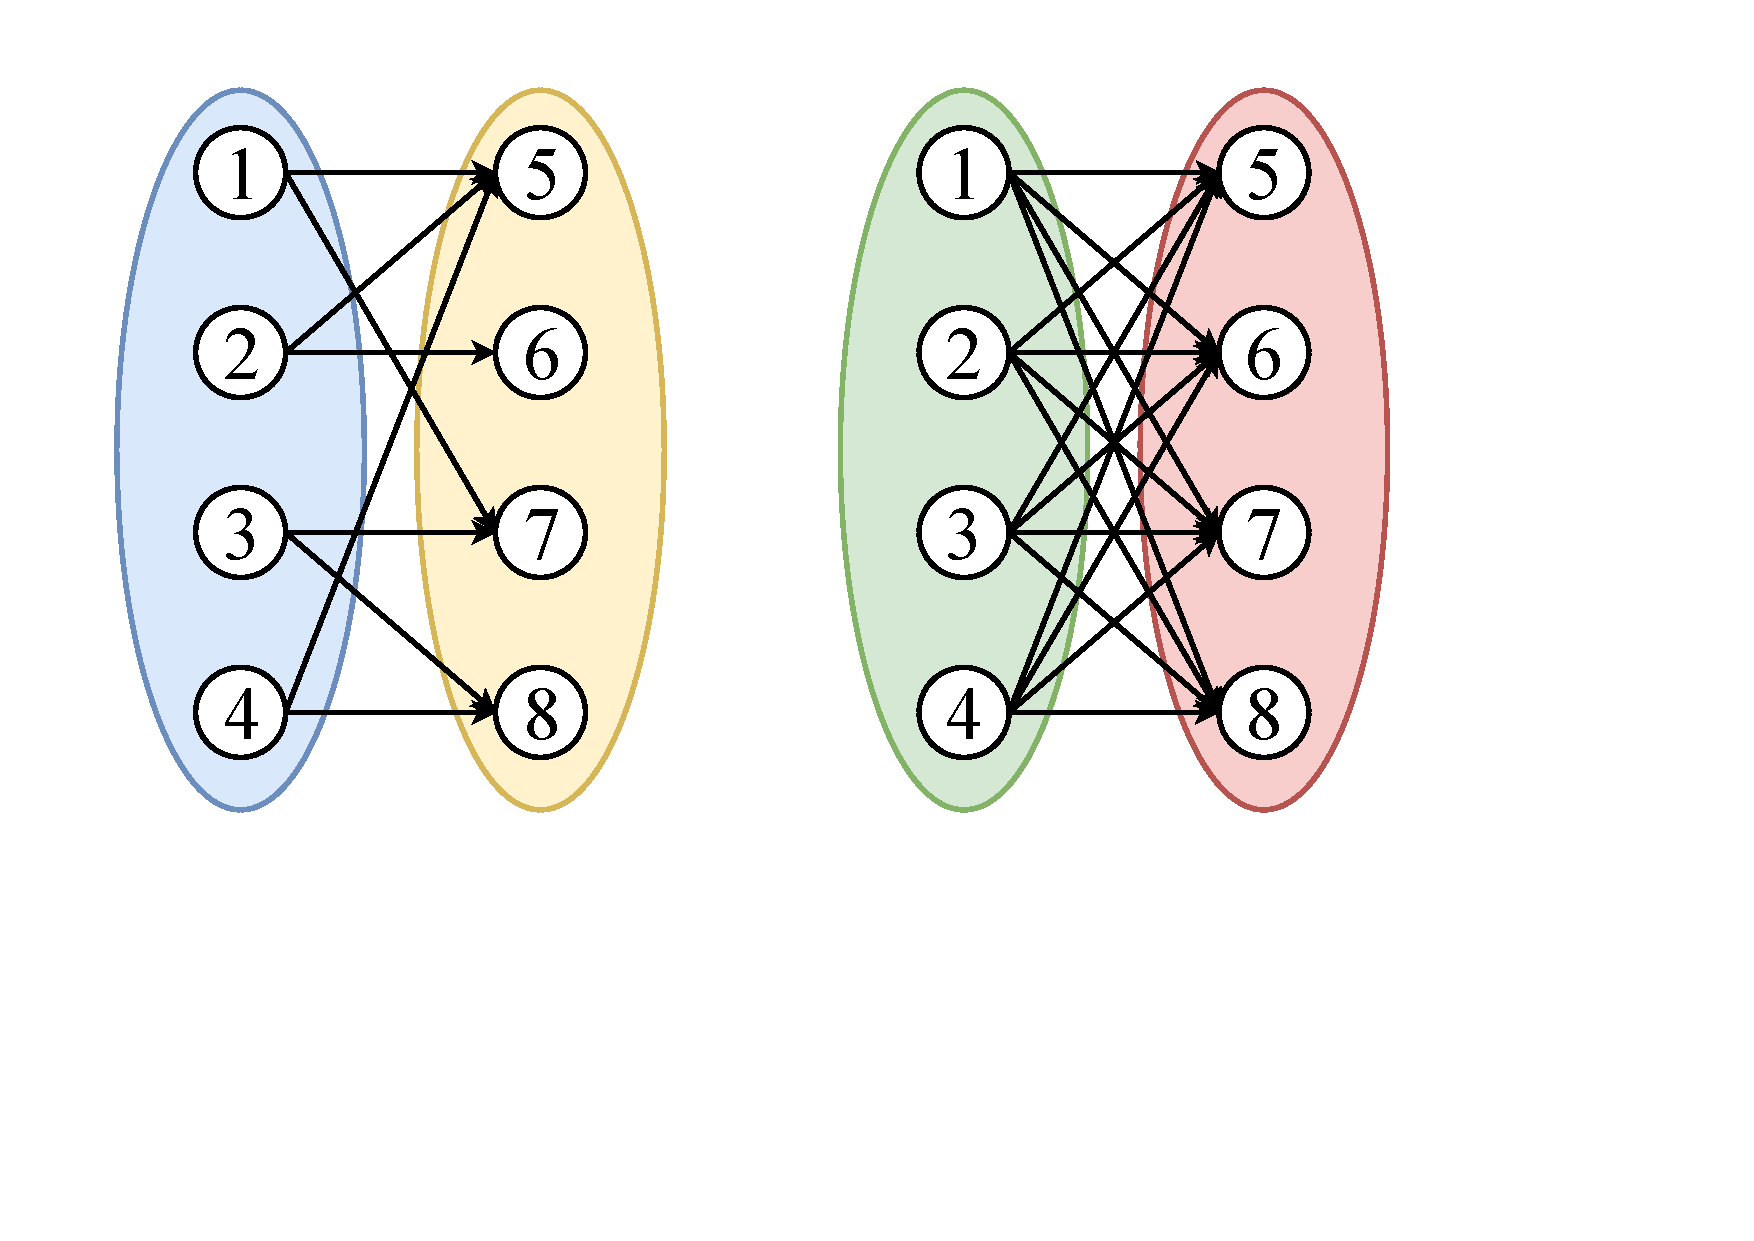
\includegraphics[scale=.3, clip,  trim=50 200 520 30]{img/graphs-bipartito.pdf}
    		
    		(a)
    	\end{minipage}
    	\begin{minipage}{0.45\textwidth}
    		\centering
    		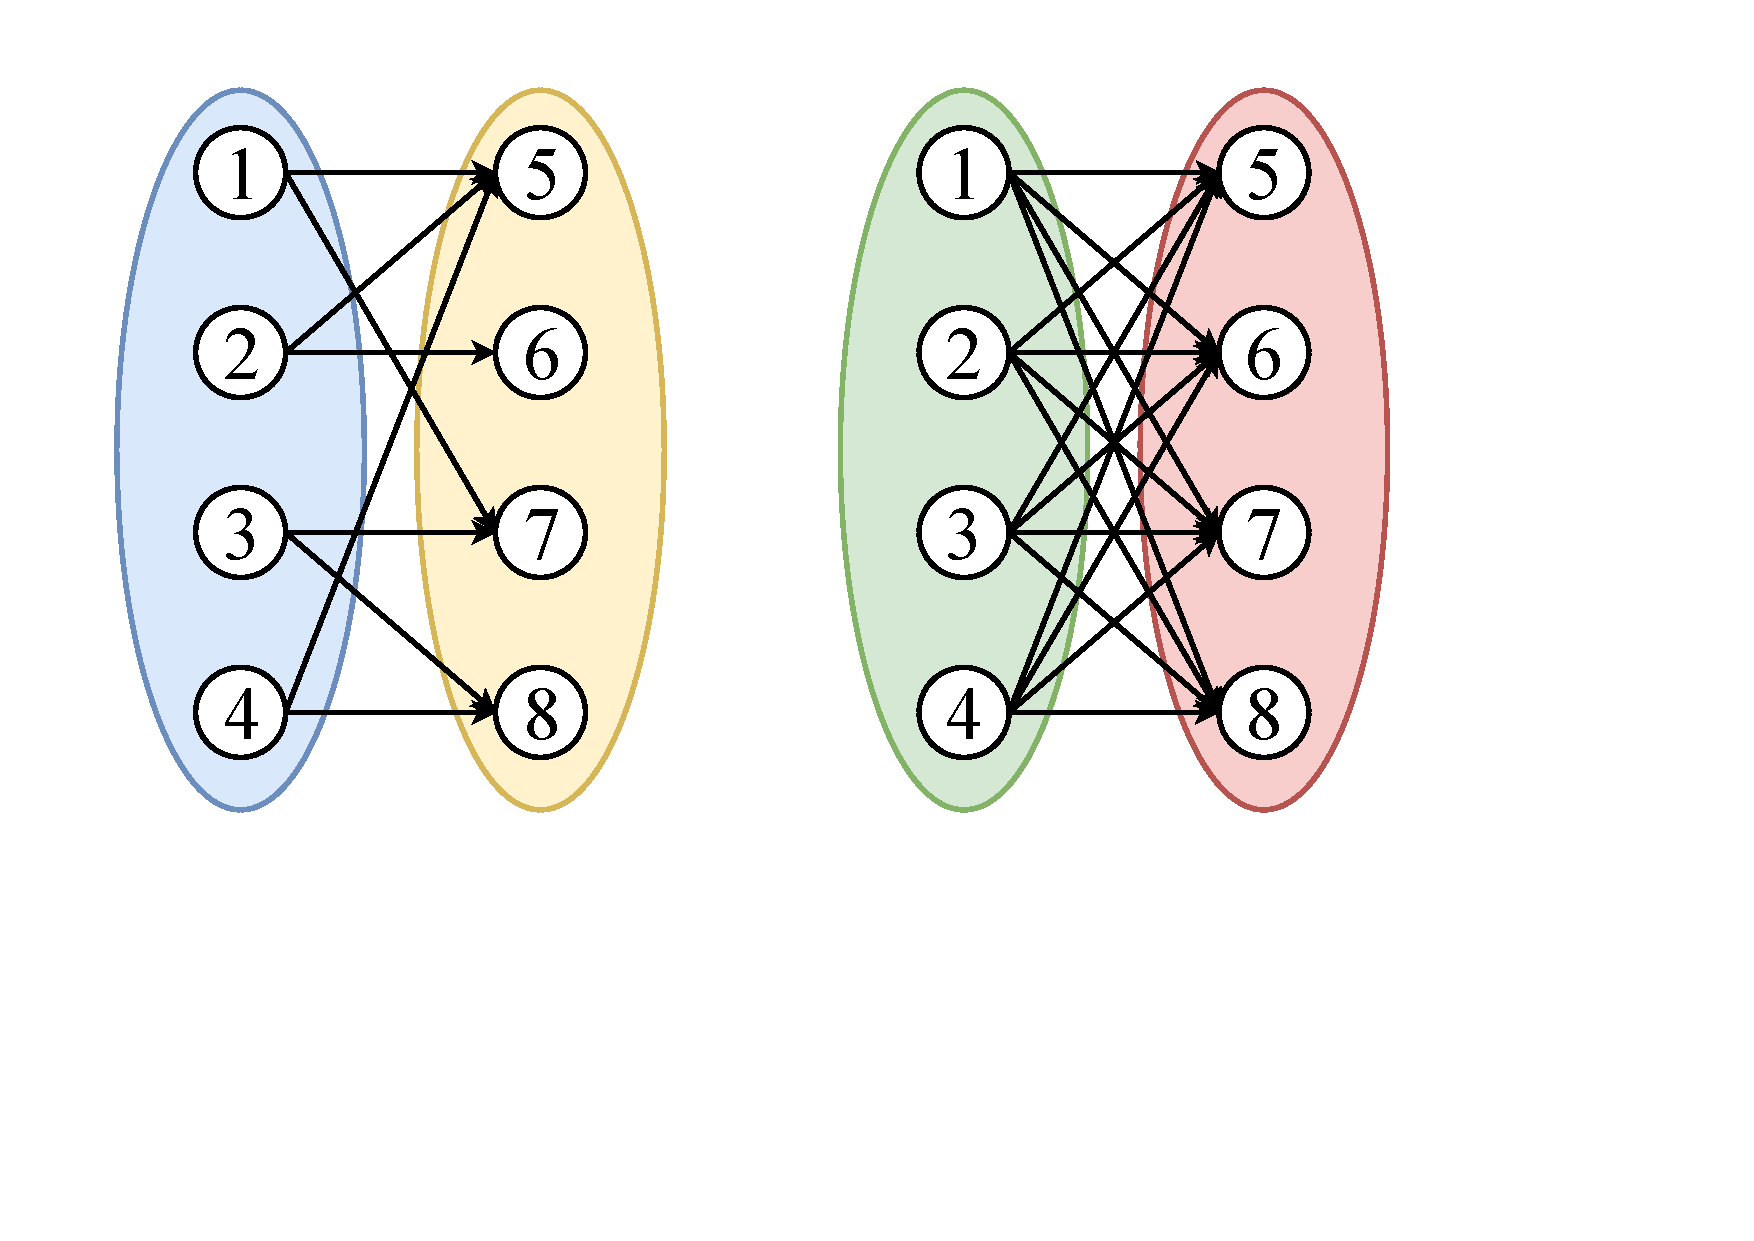
\includegraphics[scale=.3, clip, trim=400 200 170 30]{img/graphs-bipartito.pdf}
    		
    		(b)
    	\end{minipage}

    \caption{Ejemplo de grafos bipartitos. (a) Grafo bipartito. (b) Grafo bipartito completo o biclique.}
    \label{fig:bipartito}
\end{figure}


Un grafo \textbf{k-degenerate} es un grafo no dirigido donde cada subgrafo tiene un vértice con grado a lo más \textbf{k}. El índice de \textbf{degeneracy} de un grafo, $D(G)$, es el menor valor \textbf{k} para el cual el grafo es \textbf{k-degenerate}.

Un grafo \textbf{bipartito} es un grafo tal que sus vértices pueden ser particionados en dos conjuntos independientes, es decir, que los elementos de cada partición no son adyacentes entre sí. Un grafo es \textbf{bipartito completo} o \textbf{biclique}, cuando todos los vértices de un conjunto son vecinos directos de todos los vértices del otro conjunto. En la \autoref{fig:bipartito} se ilustra un ejemplo de grafo bipartito y un biclique.
%Un grafo \textbf{bipartito} cuando sus vértices se pueden separar en dos conjuntos separados $U$ y $W$, tal que se cumple $U \cup W = V$ y $U \cap W = \varnothing$. Un grafo es \textbf{bipartito completo} o \textbf{biclique}, cuando todos los vértices de un conjunto son vecinos directos de todos los vértices del otro conjunto. En la \autoref{fig:bipartito} se ilustra un ejemplo de grafo bipartito y un biclique.

Un \textbf{clique} es un subgrafo donde todos los vértices son adyacentes entre sí, es decir, $\exists V' \subseteq V(G), \forall v_{1}, v_{2} \in V', (v_{1}, v_{2}) \in E(G) $. Un \textbf{clique maximal} no puede extenderse incluyendo otro vértice adyacente, es decir, no es subconjunto de otro clique más grande. En la \autoref{fig:maxCliqueExample} se presenta ejemplo de un grafo y sus cliques maximales.

\begin{figure}
    	\centering
    	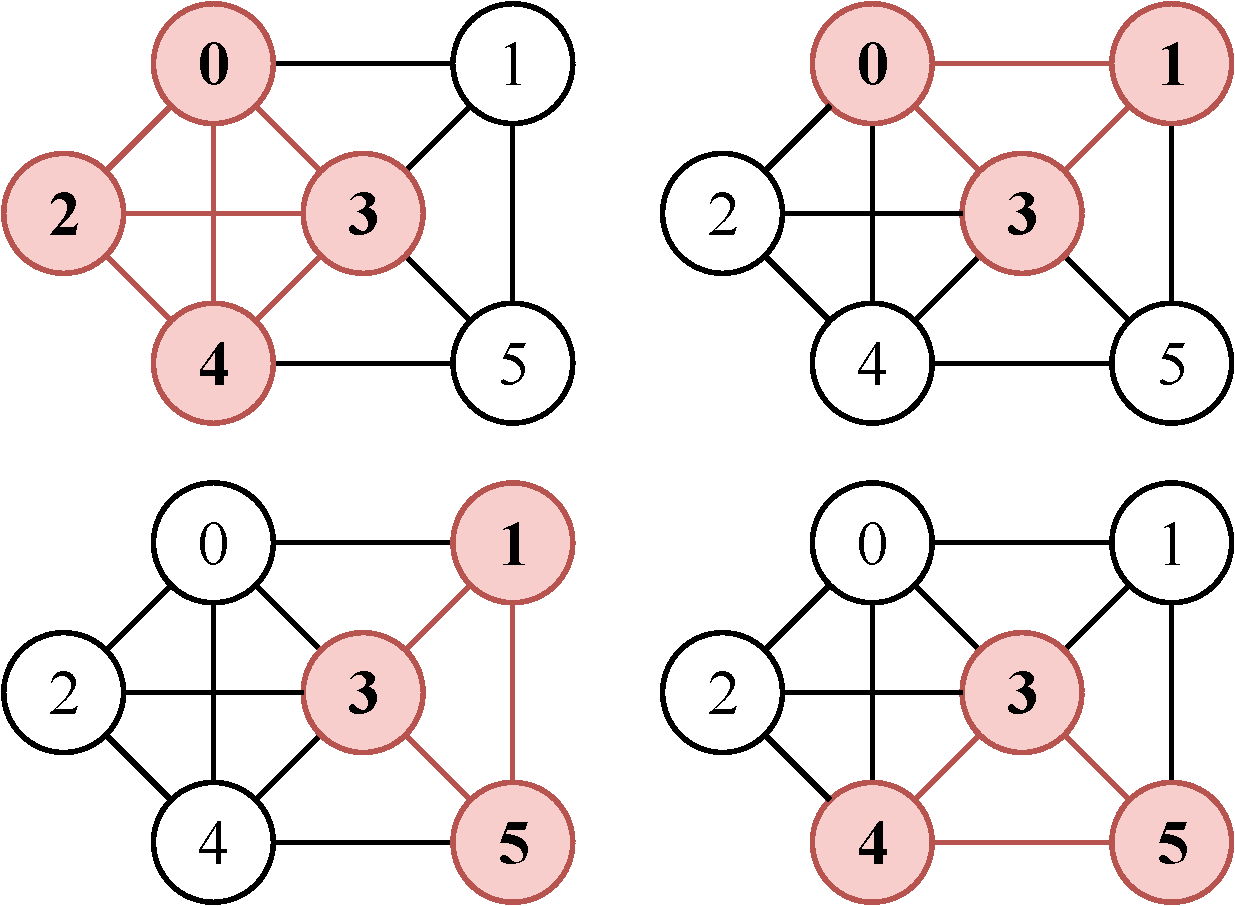
\includegraphics[width=0.5\linewidth]{img/maxCliqueExample.pdf}
    	
    \caption{Ejemplo de grafo y sus cliques maximales.}
    \label{fig:maxCliqueExample}
\end{figure}


Un \textbf{triángulo} es un subgrafo de tres vértices y tres aristas. Se define $\lambda(v)$ como la cantidad de triángulos donde participa un nodo $v$, y $\lambda(G)$ como la cantidad de triángulos de un grafo, y se calcula sumando el cálculo individual para cada vértice, y dividiendo el total en tres (por cada triángulo se cuentan 3 veces los vértices), como lo muestra la siguiente ecuación

\begin{equation}
	\lambda(G) = \dfrac{1}{3} \sum_{v \in V} \lambda(v) \label{eq:triangles}
\end{equation}

Un \textbf{triplete} es un subgrafo de tres vértices y dos aristas, donde las aristas comparten un vértice común. Se define $\tau(v)$ como la cantidad de tripletes donde $v$ es el vértice común, y $\tau(G)$ como la cantidad de tripletes de un grafo.

\begin{equation}
	\tau(G) = \sum_{v \in V} \tau(v) \label{eq:triplets}
\end{equation}

El \textbf{coeficiente de clusterización} de un vértice indica cuánto está conectado con sus vecinos, y se define como $c(v) =  \lambda(v) / \tau(v)$. El coeficiente de clusterización de un grafo ($C(G)$) es el promedio del coeficiente de todos los nodos del grafo, y se define como:

\begin{align}
	C(G) &= \dfrac{1}{|V'|} \sum_{v \in V'} c(v) \label{eq:CC} \\
	V' &= \{ v \in V | d(v) \geq 2 \} \nonumber
\end{align}

\noindent donde $V'$ es el conjunto de vértices con un grado mayor a dos. Su rango es entre $[0, 1]$, mientras más cercano a $1$ indica más conexión entre vértices.

La \textbf{transitividad} de un grafo ($T(G)$) es la probabilidad que un par de nodos adyacentes estén interconectados, y se define como:

\begin{equation}
	T(G) = \dfrac{3 \lambda(G)}{\tau(G)} \label{eq:T} 
\end{equation}

\noindent y su rango también va entre $[0, 1]$, siendo $1$ cuando todos los nodos están interconectados con todos.

Tanto el coeficiente de clusterización como la transitividad son métricas que permiten vislumbrar cuán conectados o clusterizados están los vértices de un grafo, y de sus ecuaciones se puede notar que están relacionados.

\section{Codificaciones}

Existen distintos tipos de codificaciones, según la aplicación. En esta sección se resumen algunas de relevancia para este trabajo, como algunos códigos universales o la codificación Huffman.

\subsection{Códigos universales}\label{sec:Ucoding}
Los códigos universales para enteros son un tipo de códigos que transforman enteros positivos en secuencias de bits, donde el largo de la secuencia final de bits tiene relación con el entero a codificar. Existen varios códigos de este tipo, algunos son:

\begin{itemize}
	\item \textbf{Código unario}: Se representa un entero $x$ por una secuencia de $1^{x-1}0$, donde el $0$ indica el término de la secuencia. Por ejemplo, el número $5$ se representa por la secuencia $11110$. Este código no es muy eficiente por si solo, pero se usa de base para otro tipo de códigos.
	
	\item \textbf{Código gamma ($\gamma$)}: Se representa un entero $x$ en un par concatenado de \textit{largo} y \textit{offset}. \textit{Offset} es la representación binaria de $x$, pero sin el primer 1. Por ejemplo, para $x=5$ su representación binaria es $101$, por tanto su \textit{offset} es $01$. \textit{Largo} codifica el largo de \textit{offset} en código unario. Para $x=5$, el largo de \textit{offset} es 2 bits, por tanto \textit{largo} es $110$. Concatenando ambas, el código $\gamma$ para $x=5$ es $11001$.
	
	\item \textbf{Código delta ($\delta$)}: Este código es una extensión del código $\gamma$ para enteros largos. Básicamente hacen lo mismo, pero el \textit{largo} lo representan en código $\gamma$ en vez de código unario. El código $\delta$ para $x=5$ es $10001$.
\end{itemize}

\subsection{Codificación Huffman}\label{sec:huffman}
La codificación Huffman\cite{huffman1952method} es un técnica de compresión de datos óptima que define códigos de largo variable libre de prefijos. Es óptima porque el tamaño de la representación comprimida es mínima y es libre de prefijos porque ningún código es prefijo de otro. Huffman es un algoritmo greedy basado en definir códigos mas cortos para aquellos elementos mas frecuentes. 

Una codificación binaria de largo fijo, le asigna la misma cantidad de bits a todos los símbolos por codificar. Una de largo variable le asigna menos bits a los símbolos más frecuentes, y más bits a los menos frecuentes, cuidando que las secuencias binarias cortas no sean prefijos de las más largas. La \autoref{fig:fixedVarLength} se tiene la frecuencia de seis símbolos en una secuencia de 100.000 caracteres, y se comparan ambos códigos. Para el caso de largo fijo, se requieren 3 bits por cada símbolo en la secuencia, un total de 300.000 bits. Para el caso de largo variable, el símbolo más frecuente \texttt{a} requiere un bit, y los menos frecuentes requieren 4 bits. Así, la secuencia requiere:

\begin{align*}
	(45 \cdot 1 + 13 \cdot 3 + 12 \cdot 3 + 16 \cdot 3 + 9 \cdot 4 + 5 \cdot 4) \cdot \textrm{1.000} = \textrm{224.000 bits}
\end{align*}

\noindent lo que significa una reducción cercana al $20\%$. 

Un código prefijo es aquel donde ninguna palabra codificada es usada como prefijo de otra. Estos códigos son simples de decodificar, basta con comenzar el proceso desde el primer bit hasta encontrar una de las posibles codificaciones, traducirla a su valor original, y seguir con el resto de bits codificados. Siguiendo el ejemplo, la secuencia $001011101$ se identifica como $0 \cdot 0 \cdot 101 \cdot 1101$, y se traduce como \texttt{aabe}.

Para agilizar la búsqueda, el código prefijo se puede representar como un árbol binario, donde los nodos hojas son los caracteres codificados. Siguiendo cada bit de la secuencia, se puede ir avanzando por el árbol hasta llegar a un nodo hoja, y así llegar al valor buscado. En la \autoref{fig:fixVarTrees} se ilustran los árboles de las codificaciones de la \autoref{fig:fixedVarLength}, en (a) el correspondiente a código de largo fijo, y en (b) el de largo variable.

 \begin{figure}[b]
    	\centering
    
    \begin{tabular}{l|cccccc}
    		& a & b & c & d & e & f \\
    		\midrule
    		Frecuencia (en miles) & 45 & 13 & 12 & 16 & 9 & 5 \\
    		Código largo fijo & 000 & 001 & 010 & 011 & 100 & 101 \\
    		Código largo variable & 0 & 101 & 100 & 111 & 1101 & 1100 \\
    \end{tabular}

    \caption{Ejemplo de códigos de largo fijo y largo variable.}
    \label{fig:fixedVarLength}
\end{figure}


\begin{figure}[b]
    	\centering
    	\begin{minipage}{0.45\textwidth}
    		\centering
    		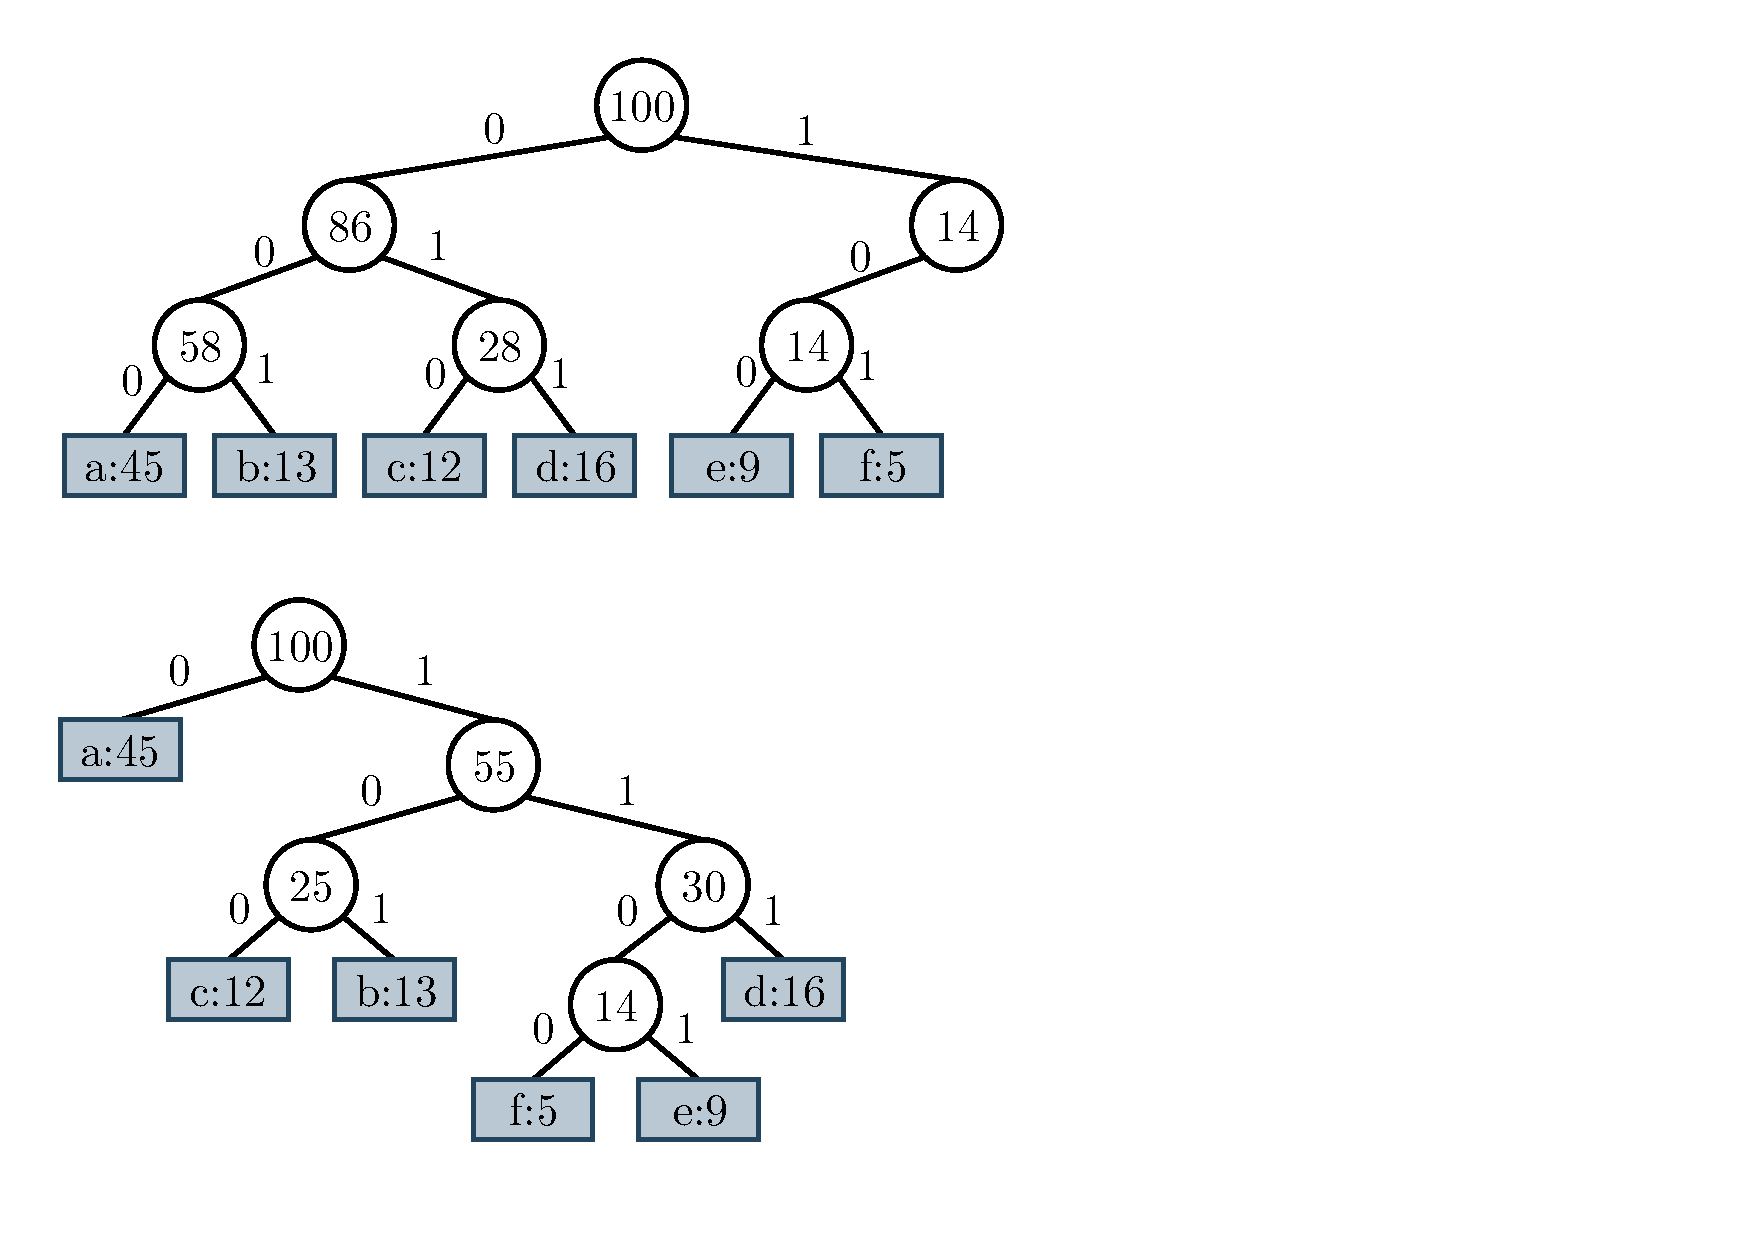
\includegraphics[scale=.45, clip,  trim=20 350 350 20]{img/graphs-fixVarTrees.pdf}
    		
    		(a)
    	\end{minipage}
    	\begin{minipage}{0.45\textwidth}
    		\centering
    		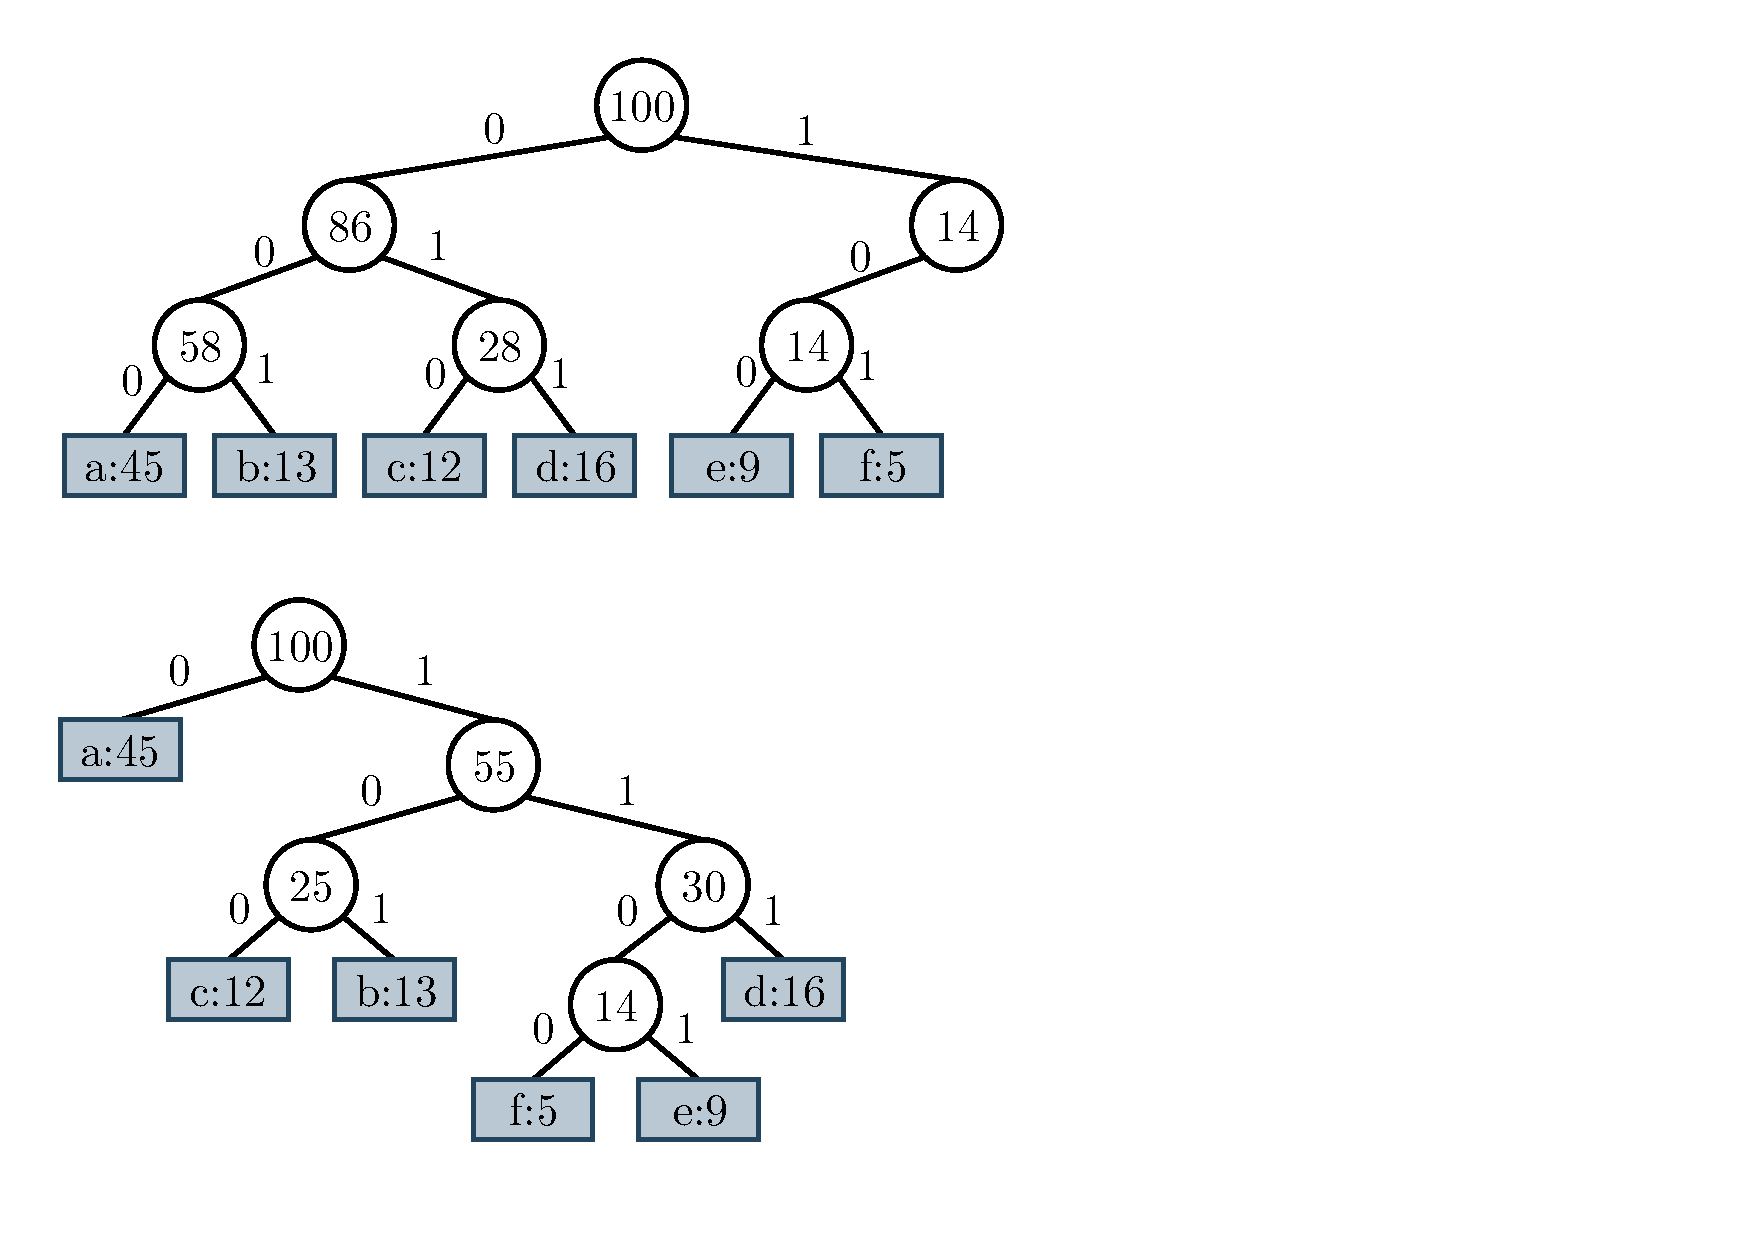
\includegraphics[scale=.45, clip, trim=20 40 430 280 ]{img/graphs-fixVarTrees.pdf}
    		
    		(b)
    	\end{minipage}

    \caption{Árboles correspondientes a los códigos de la Figura~\ref{fig:fixedVarLength}. (a)~Árbol para código de largo fijo. (b)~Árbol para código de largo variable.}
    \label{fig:fixVarTrees}
\end{figure}


La codificación Huffman aprovecha todo lo anterior, utilizando una heurística \textit{greedy} para la construcción de su estructura y su compresión final. Asumiendo que se tiene una secuencia $C$ de $n$ caracteres, y que cada carácter $c \in C$ tiene una frecuencia $f[c]$ en $C$. El algoritmo crea un árbol desde los nodos hojas hacia el nodo raíz, inicialmente con $|C|$ hojas, y ejecutando $|C| - 1$ conexiones para llegar al árbol final. Luego identifica los dos elementos menos frecuentes y los conecta a un nuevo elemento, con frecuencia igual a la suma de ambos. Esto continúa hasta que todos los nodos hojas están conectados al árbol. En la \autoref{fig:huffman2} se ilustra este proceso para la secuencia ejemplo de la \autoref{fig:fixVarTrees}(b), y a continuación se detalla el proceso:

\begin{enumerate}
	\item \textbf{\autoref{fig:huffman2}(a)}: Se crean los $|C| = 6$ nodos hoja para cada carácter.
	\item \textbf{\autoref{fig:huffman2}(b)}: Se identifican los dos nodos de caracteres menos frecuentes, $f$ con $f[f] = 5$ y $e$ con $f[e] = 9$ (en miles), y se conectan a un nuevo nodo con frecuencia $5 + 9 = 14$.
	\item \textbf{\autoref{fig:huffman2}(c)}: Los siguientes nodos menos frecuentes son $c$ con $f[c] = 12$ y $b$ con $f[b] = 13$, y se conectan a otro nodo nuevo con frecuencia $12 + 13 = 25$.
	\item \textbf{\autoref{fig:huffman2}(d)}: El nodo creado que conecta $f$ con $e$ posee la menor frecuencia ($14$), y junto al nodo $d$ con $f[d] = 16$ se conectan en un nuevo nodo con frecuencia $14 + 16 = 30$.
	\item \textbf{\autoref{fig:huffman2}(e)}: Para juntar a los nuevos nodos de menor frecuencia, $25$ y $30$ respectivamente, se crea un nuevo nodo con frecuencia $25 + 30 = 55$.
	\item \textbf{\autoref{fig:huffman2}(f)}: Finalmente, se conecta el último nodo hoja restante, $a$ con $f[a] = 45$, con el reciente nodo creado de frecuencia $55$, mediante el nodo raíz con frecuencia $45 + 55 = 100$, confirmando la correcta creación del árbol.
\end{enumerate}

Se visualiza que se crearon $|C| - 1 = 6 - 1 = 5$ nodos para conectar todo el árbol. Con este resultado, se puede reconstruir de manera secuencial una secuencia codificada, simplemente recorriendo el árbol desde el nodo raíz hasta llegar a un nodo hoja, sustituir esa subsecuencia de bits por el valor de dicho nodo, y continuar con el resto de la secuencia de igual manera hasta el final. Retomando el ejemplo de secuencia $001011101$, en la \autoref{fig:huffmanBack} se visualizan los tres casos a decodificar: en (a) los primeros bits $0$ llegan al nodo hoja de \texttt{a}, en (b) la secuencia $101$ llega al nodo \texttt{b}, y en (c) la secuencia $1101$ llega al nodo \texttt{e}, dando en (d) la equivalencia entre bits y caracteres con resultado \texttt{aabe}.

\begin{figure}
    	\centering
    	\begin{minipage}{1\textwidth}
    		\centering
    		\begin{minipage}{0.45\textwidth}
    			\centering
    			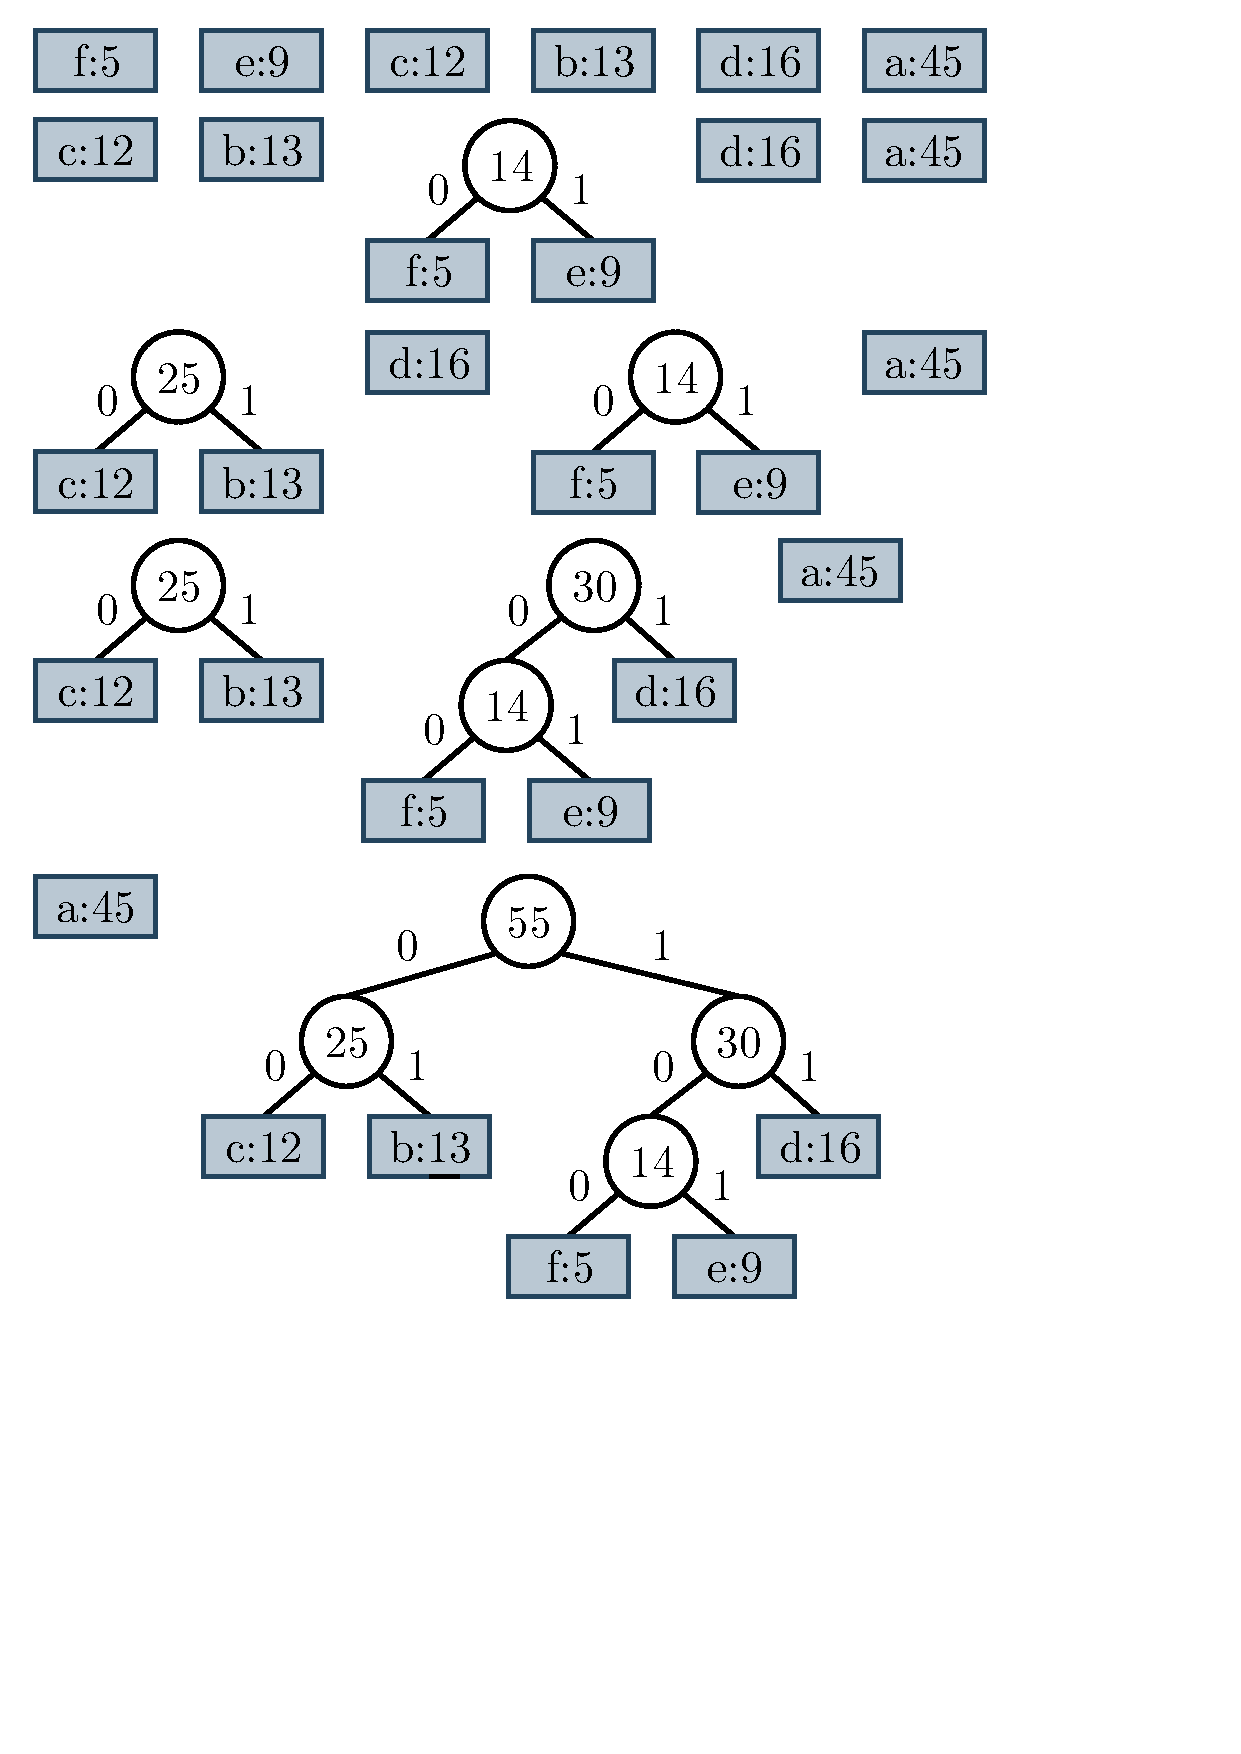
\includegraphics[scale=.45, clip, trim=16 790 120 10]{img/graphs-huffman2.pdf}
    			
    			(a)
    		\end{minipage}
    		\begin{minipage}{0.45\textwidth}
    			\centering
    			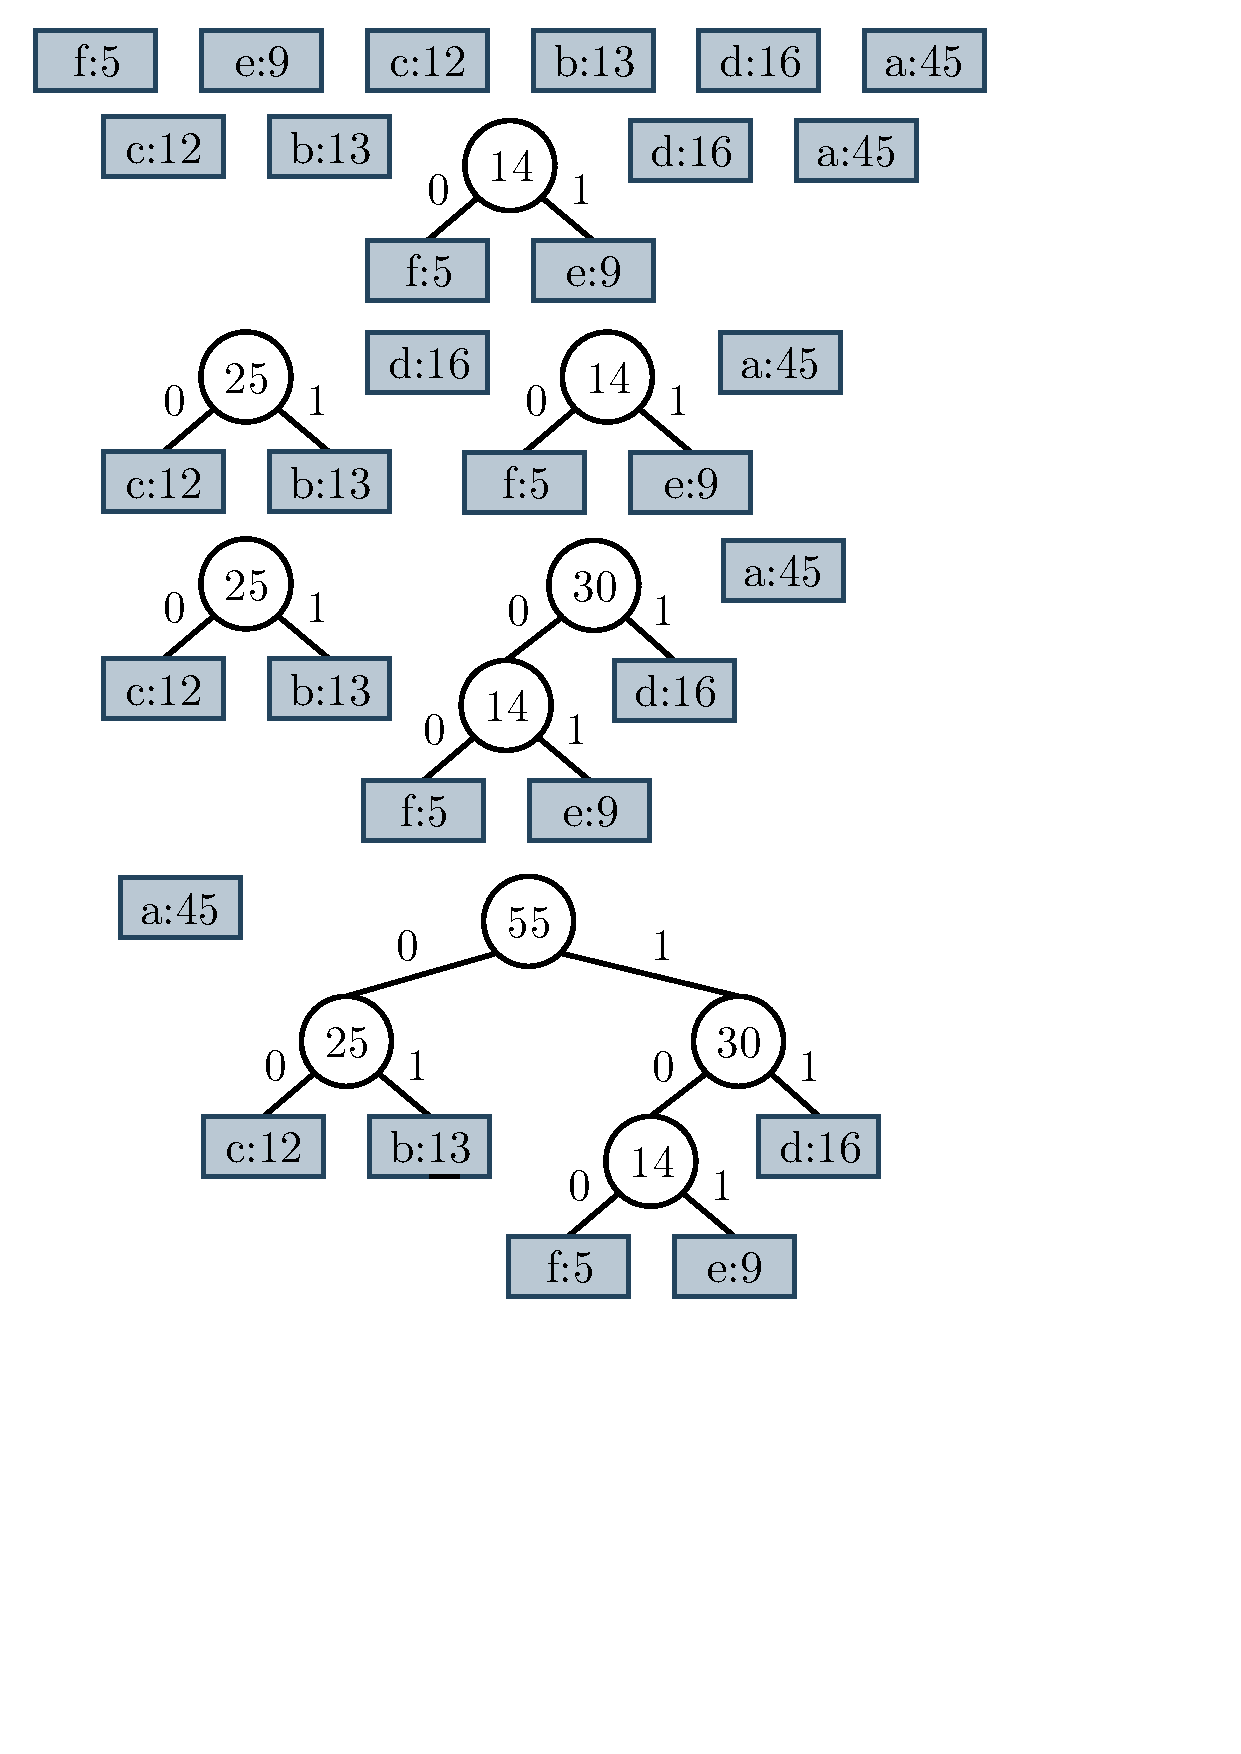
\includegraphics[scale=.45, clip, trim=40 690 150 50]{img/graphs-huffman21.pdf}

    			(b)
    		\end{minipage}  		
    	\end{minipage}
    	
    	\begin{minipage}{1\textwidth}
    		\centering
    		\begin{minipage}{0.45\textwidth}
    			\centering
    			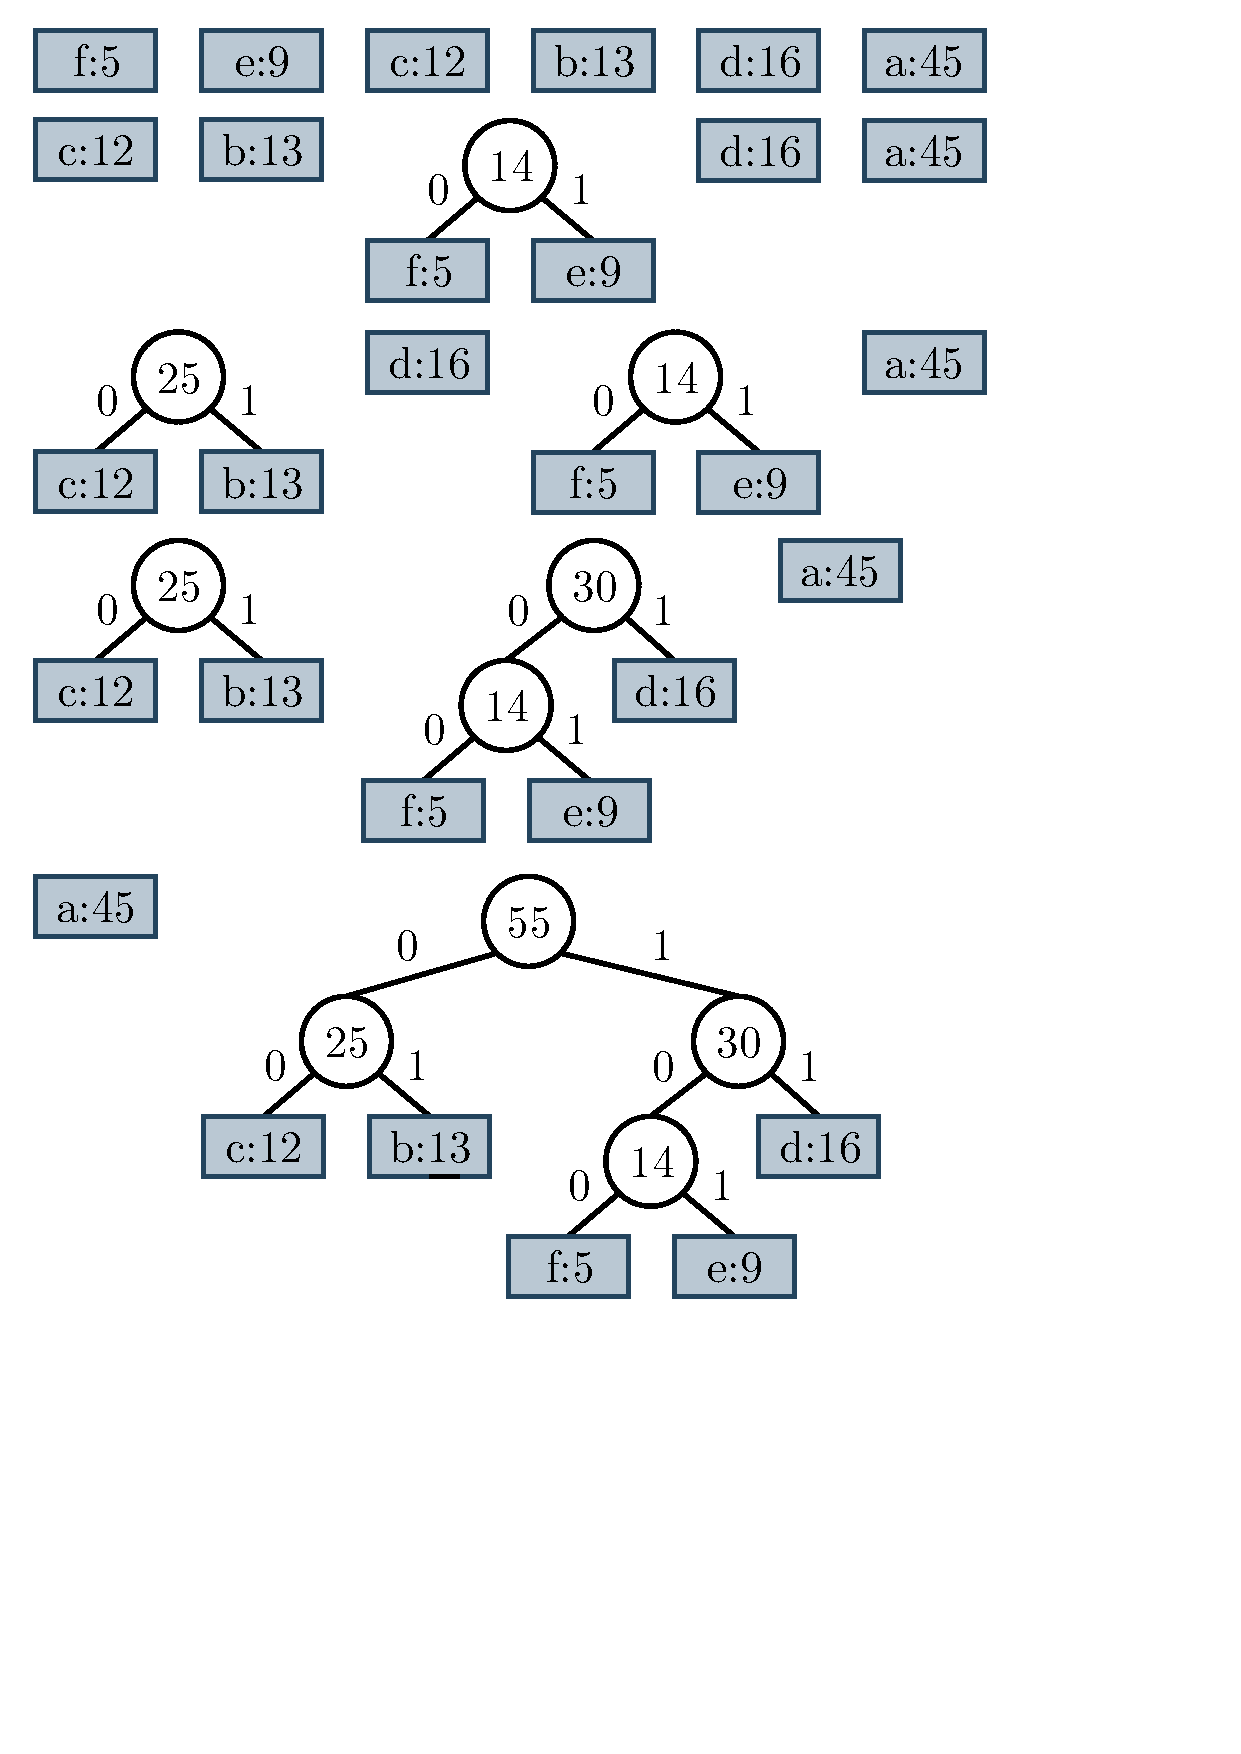
\includegraphics[scale=.4, clip, trim=10 590 120 150]{img/graphs-huffman2.pdf}
    			
    			(c)
    		\end{minipage}
    		\begin{minipage}{0.45\textwidth}
    			\centering
    			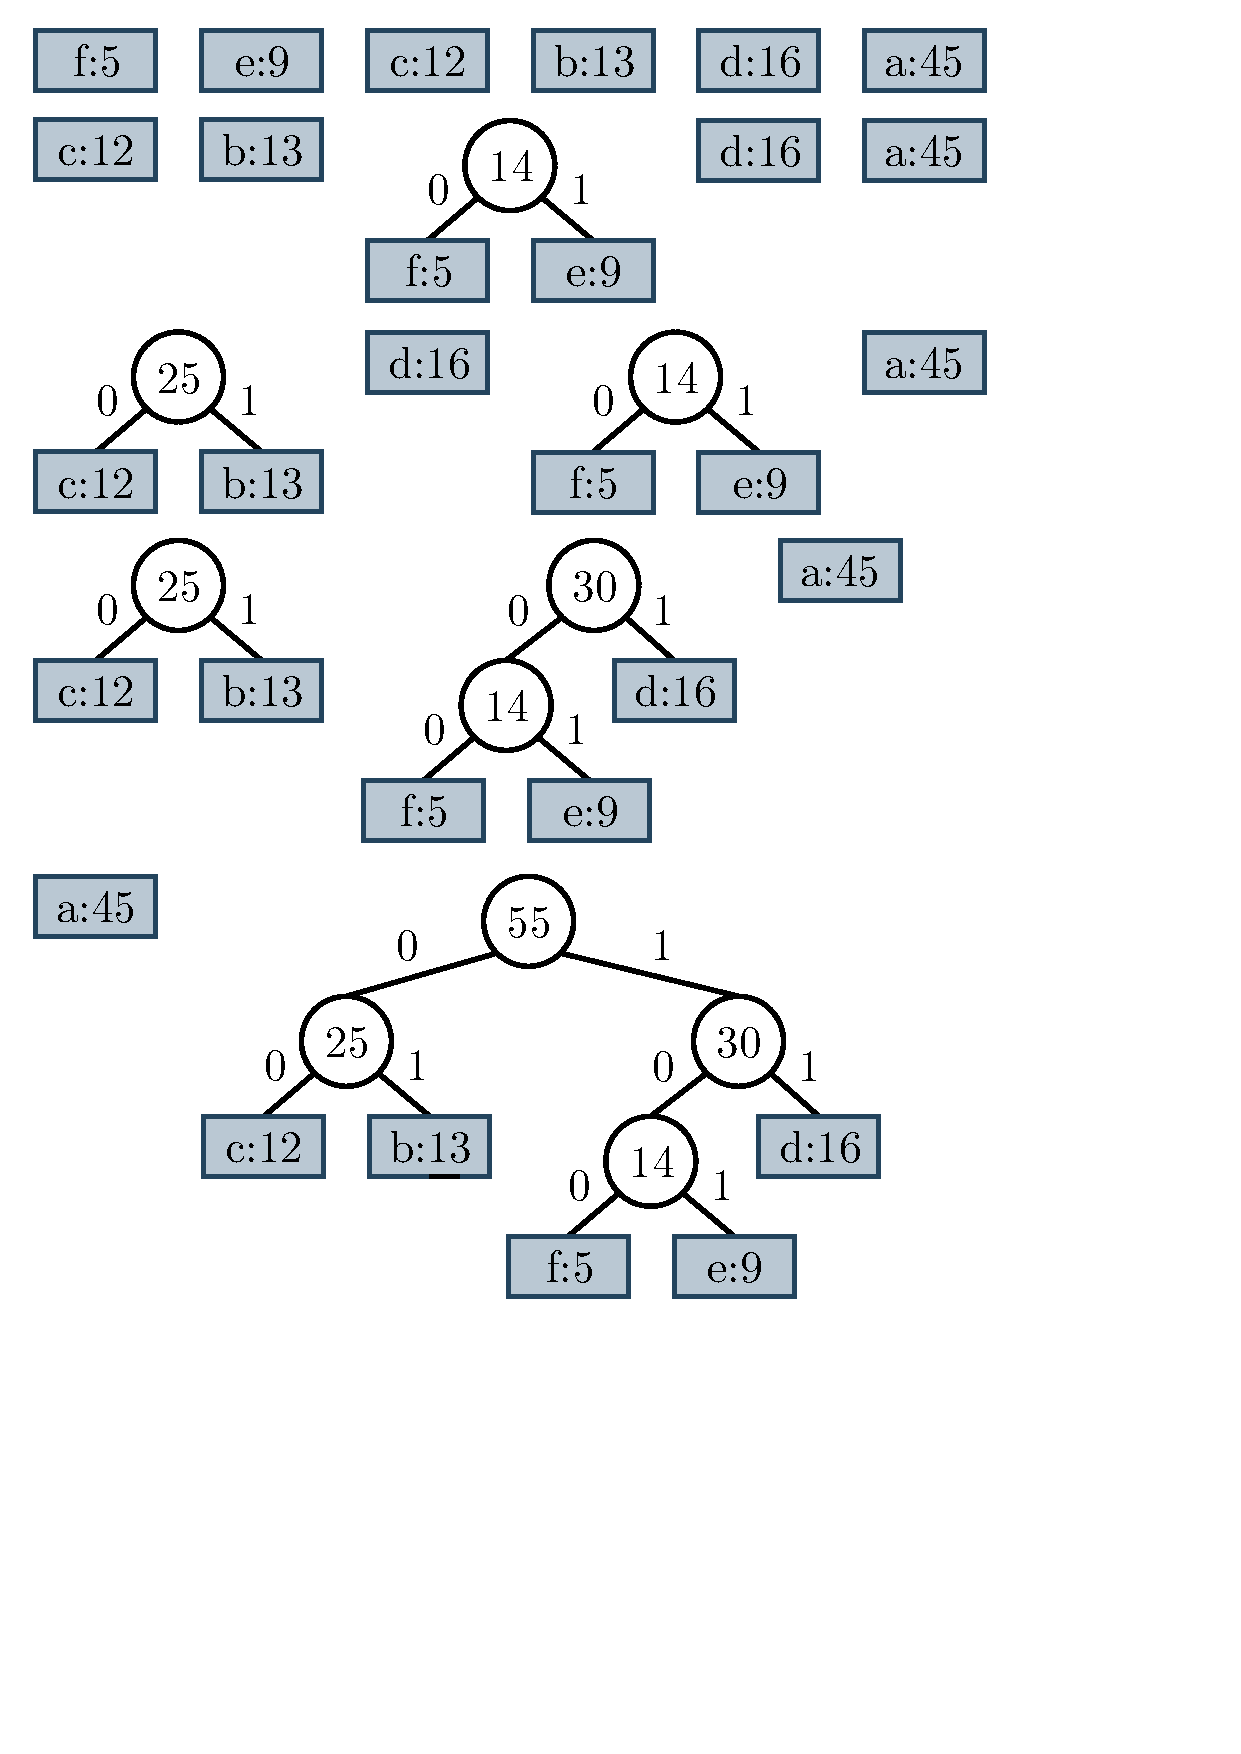
\includegraphics[scale=.4, clip, trim=10 430 160 250]{img/graphs-huffman2.pdf}
    			
    			(d)
    		\end{minipage}  
    	\end{minipage}
    	
    \begin{minipage}{1\textwidth}
    		\centering
    		\begin{minipage}{0.45\textwidth}
    			\centering
    			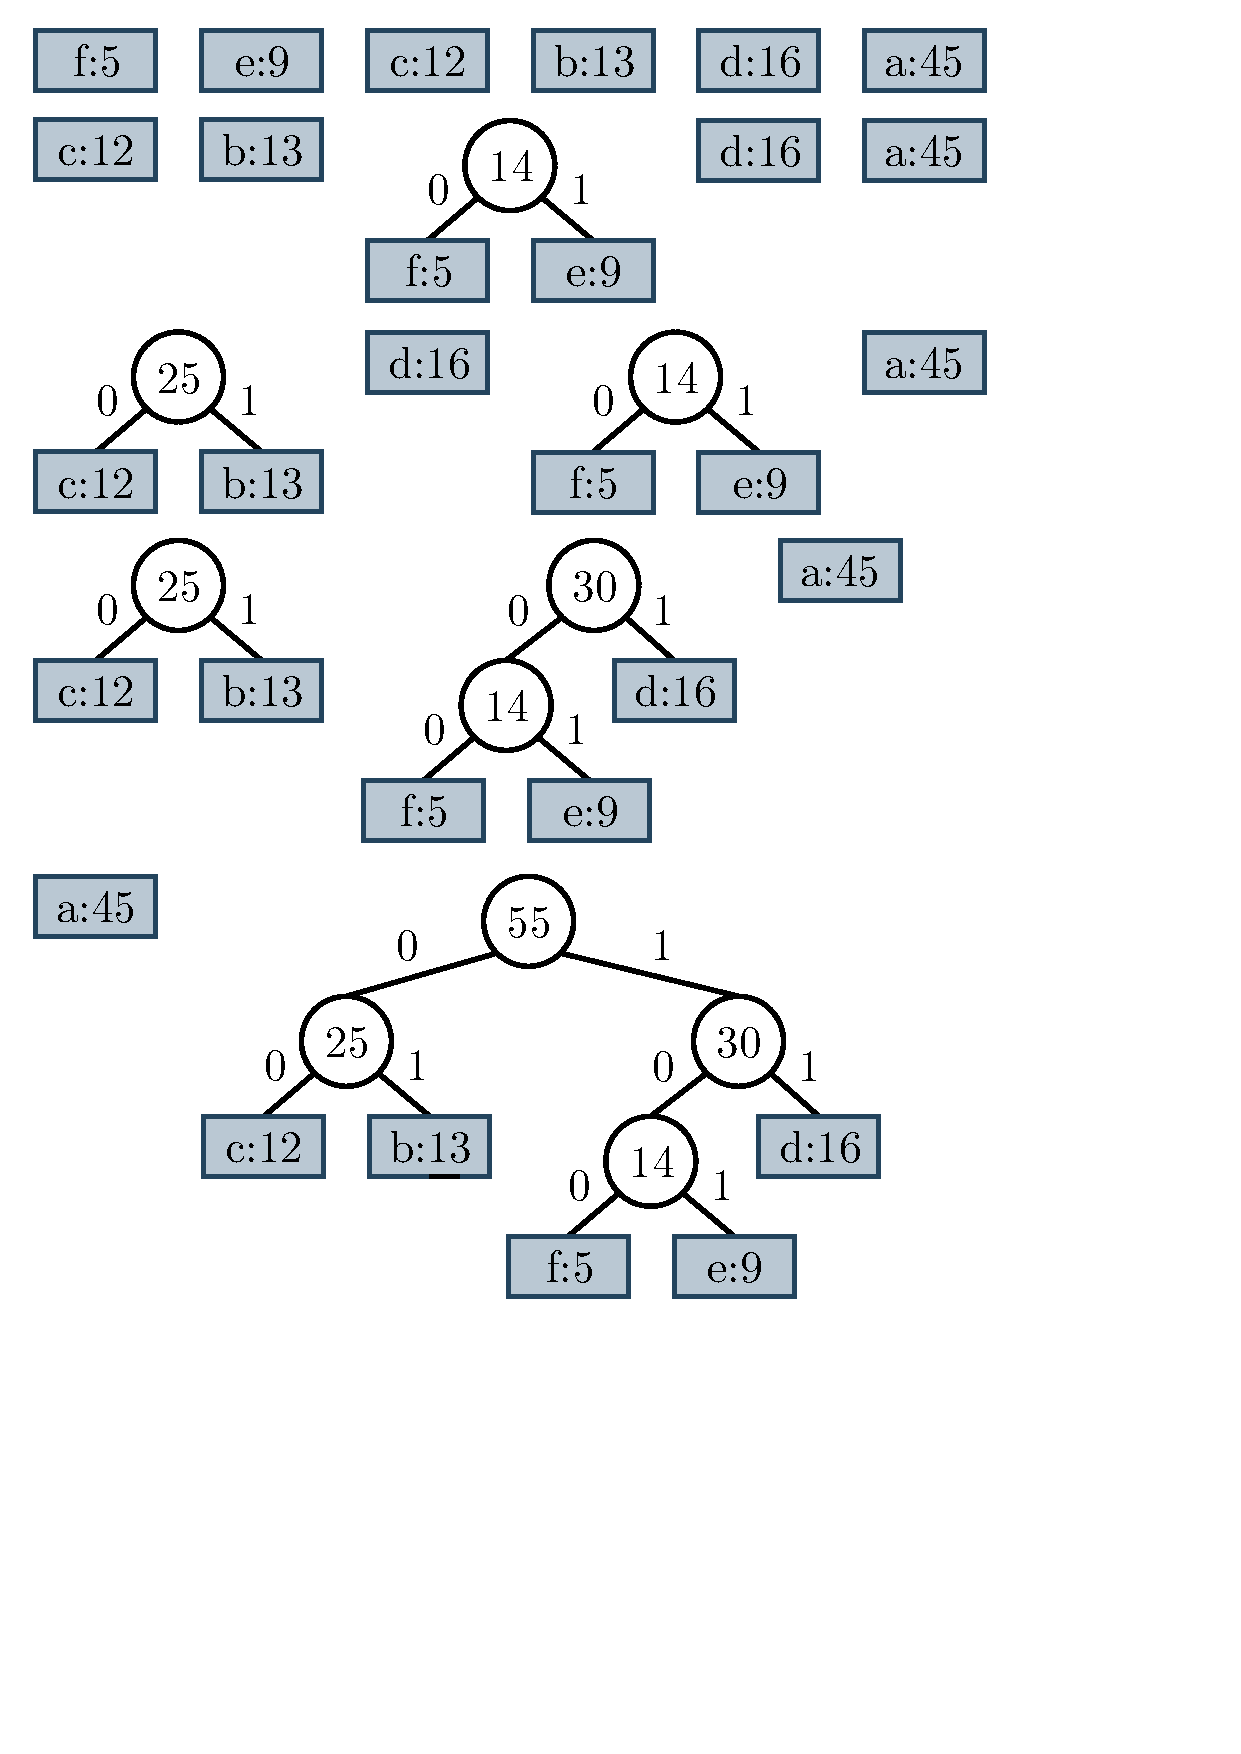
\includegraphics[scale=.4, clip, trim=10 210 170 410]{img/graphs-huffman2.pdf}
    			
    			(e)
    		\end{minipage}
    		\begin{minipage}{0.45\textwidth}
    			\centering
    			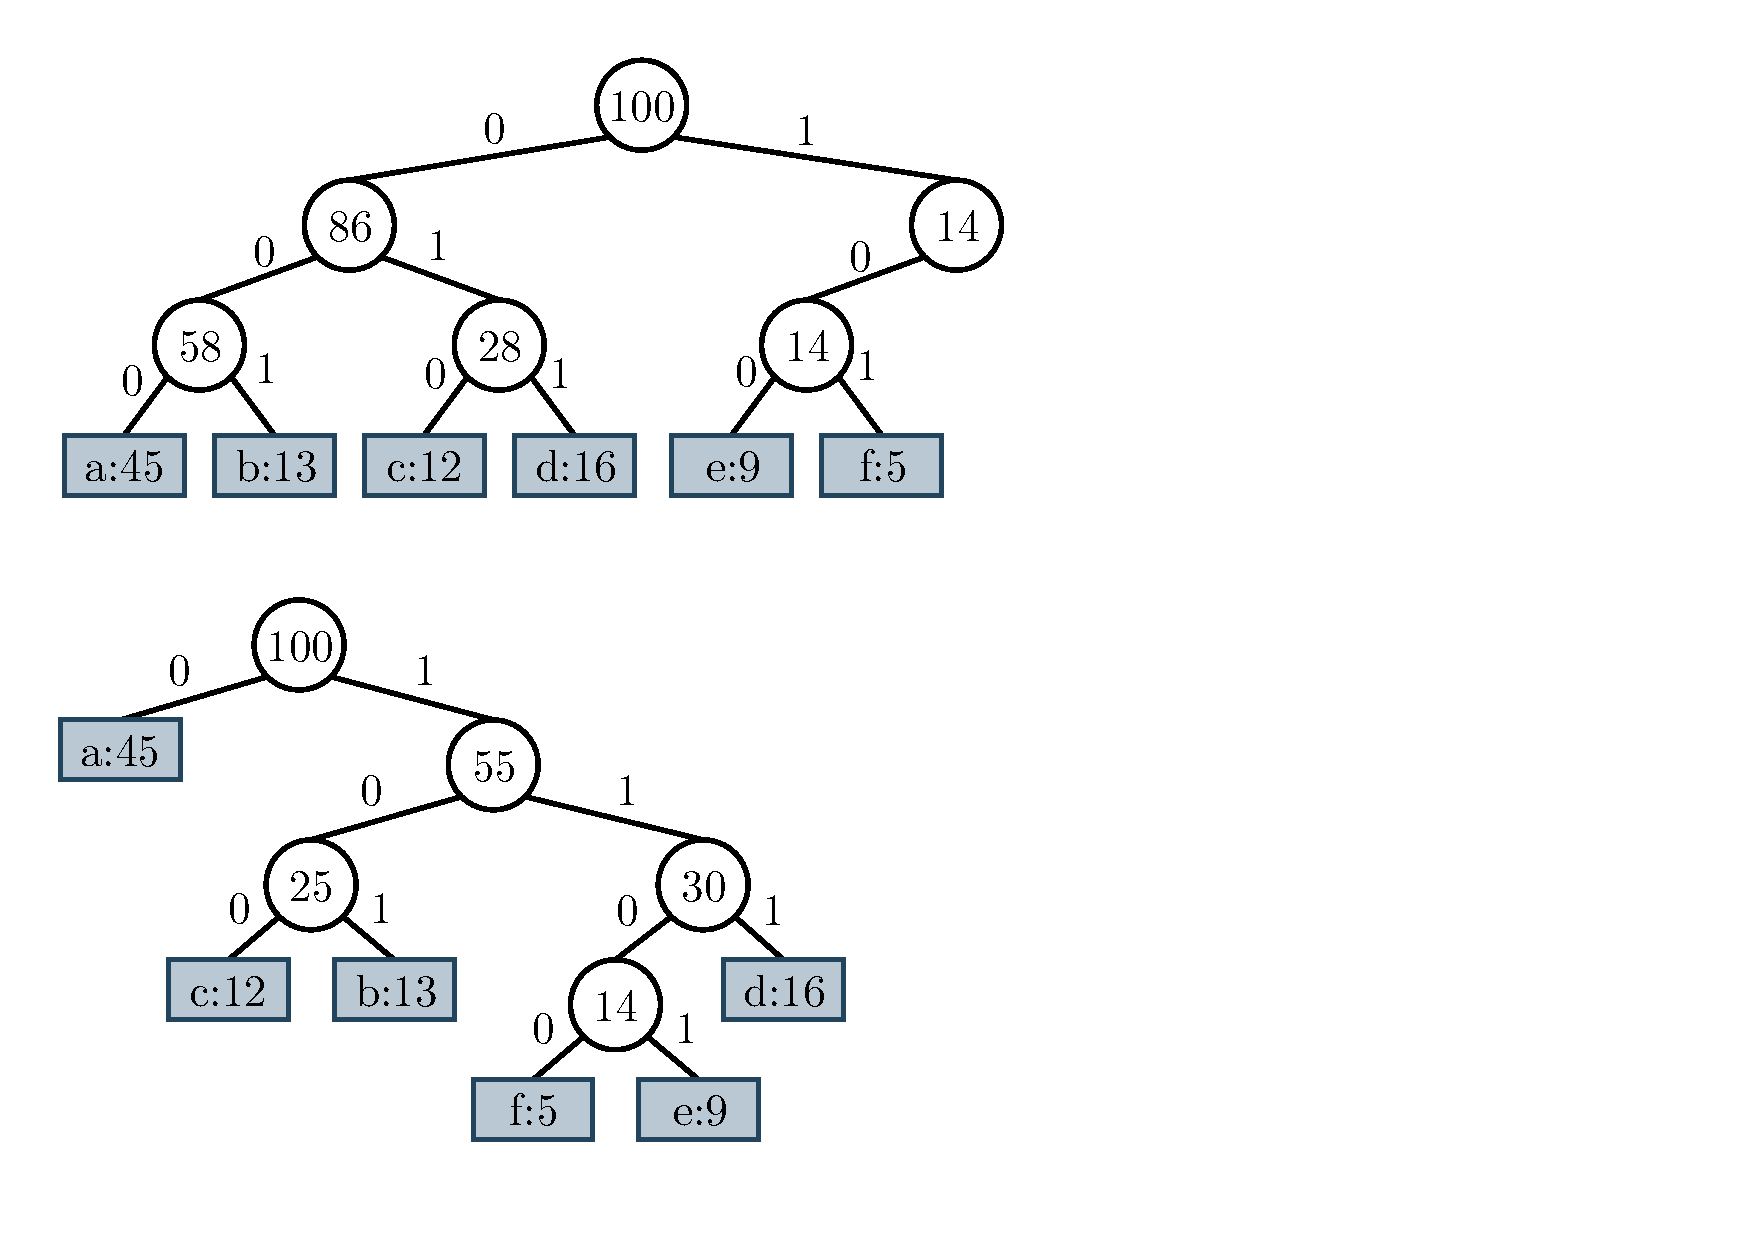
\includegraphics[scale=.4, clip, trim=20 40 430 280 ]{img/graphs-fixVarTrees.pdf}

    			(f)
    		\end{minipage}  
    	\end{minipage}
    	
    	 
    \caption{Etapas de construcción para codificación Huffman, para secuencia $C$ ejemplo. (a) Los 6 nodos hojas iniciales. (b) Primera unión. (c) Segunda unión. (c) Tercera unión. (d) Cuarta unión. (e) Quinta unión. (f) Última unión.}
    \label{fig:huffman2}
\end{figure}


\begin{figure}
    	\centering
    	\begin{minipage}{1\textwidth}
    		\centering
    		\begin{minipage}{0.45\textwidth}
    			\centering
    			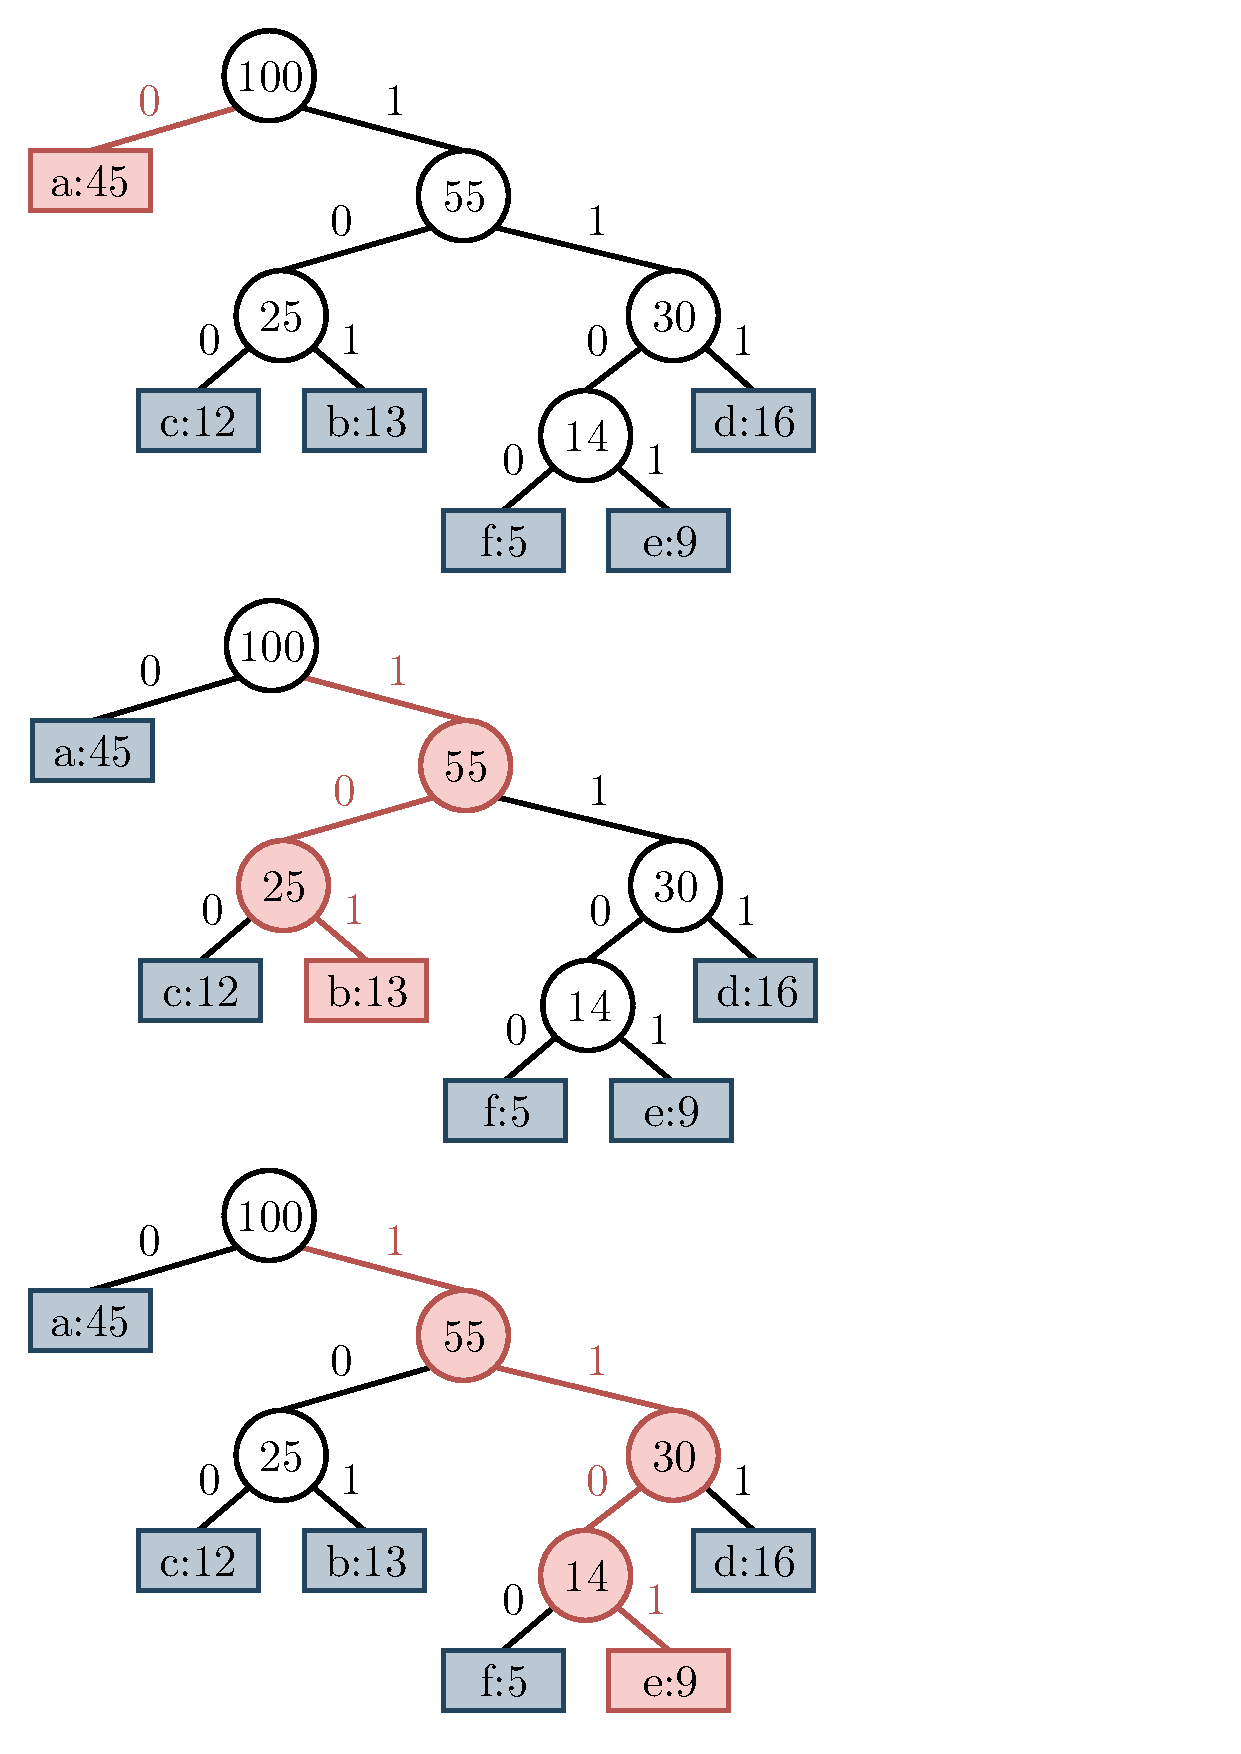
\includegraphics[scale=.45, clip, trim=10 560 200 10]{img/graphs-huffmanBack.pdf}
    			
    			(a)
    		\end{minipage}
    		\begin{minipage}{0.45\textwidth}
    			\centering
    			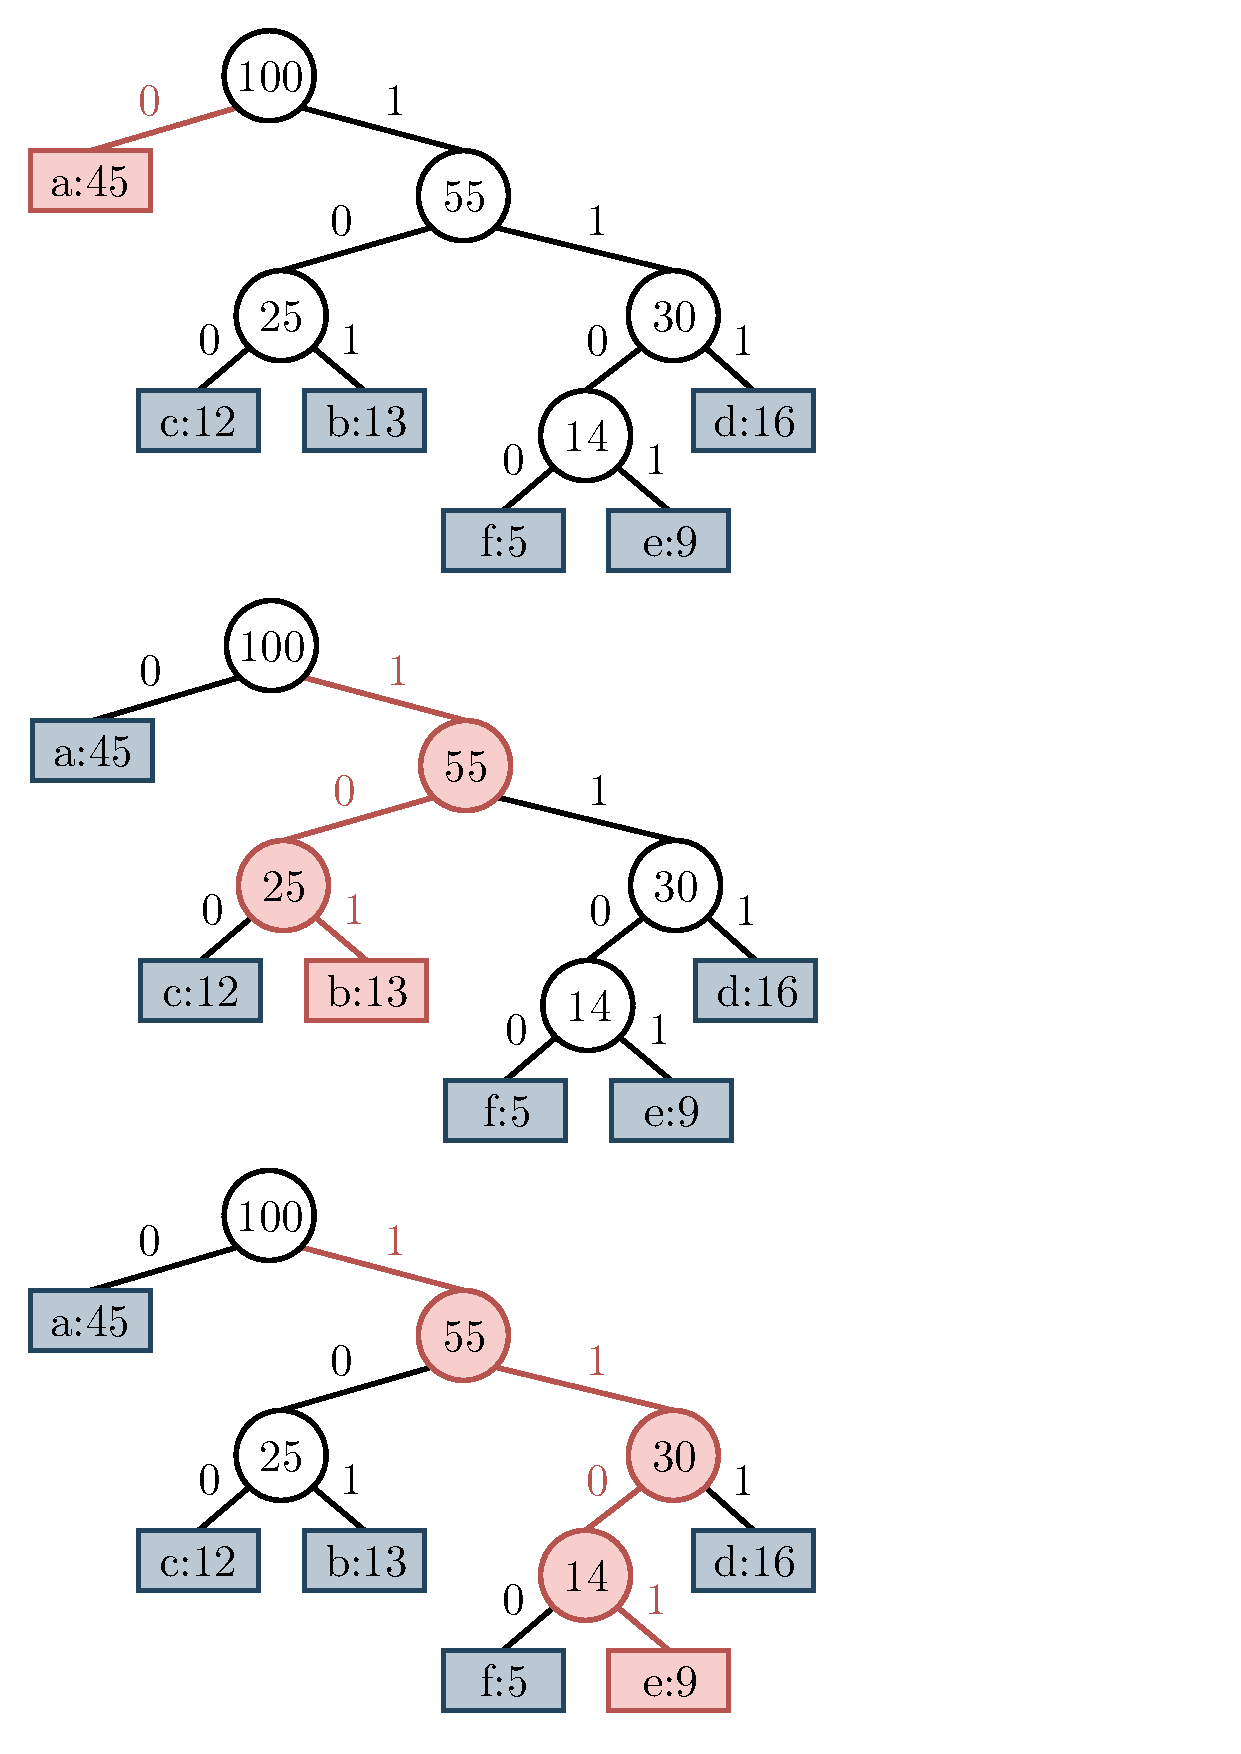
\includegraphics[scale=.45, clip, trim=10 290 200 280]{img/graphs-huffmanBack.pdf}

    			(b)
    		\end{minipage}  		
    	\end{minipage}
    	
    	\begin{minipage}{1\textwidth}
    		\centering
    		\begin{minipage}{0.45\textwidth}
    			\centering
    			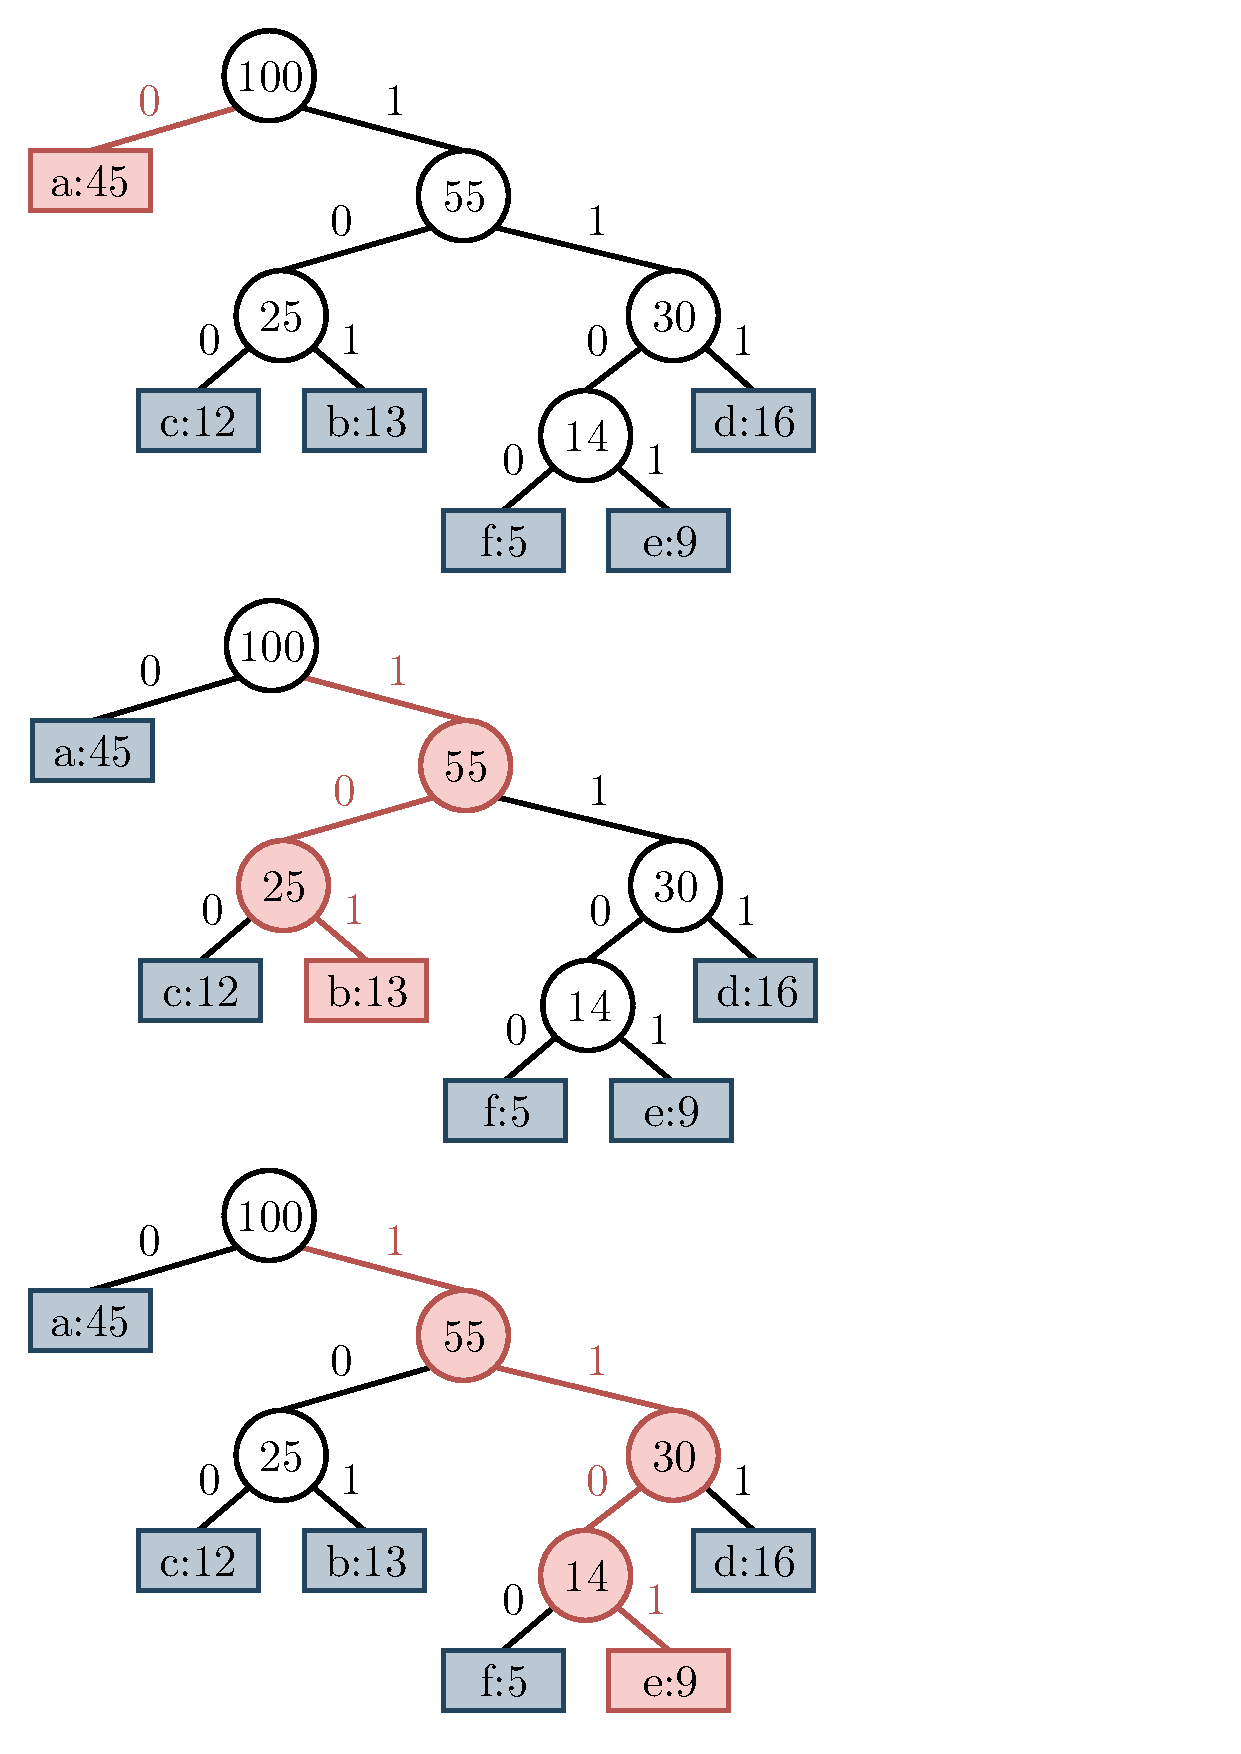
\includegraphics[scale=.4, clip, trim=10 20 200 550]{img/graphs-huffmanBack.pdf}
    			
    			(c)
    		\end{minipage}  
    		\begin{minipage}{0.45\textwidth}
    			\centering
			\begin{tabular}{cccc}
				0 & 0 & 101 & 1101 \\
				\midrule
				a & a & b & e \\
			\end{tabular}
		    	\vspace{5mm}
		    	
    			(d)
    		\end{minipage}  
    	\end{minipage}
    	
    	 
    \caption{Usando el árbol para decodificar Huffman. (a) Decodificando $0$. (b) Decodificando $101$. (c) Decodificando $1101$. (d) Equivalencias de bits y caracteres.}
    \label{fig:huffmanBack}
\end{figure}



\chapter{ESTADO DEL ARTE}\label{chap:background}
\vskip 3.0ex

En este capítulo se realiza una revisión del trabajo previo realizado en compresión de grafos, se profundiza sobre las posibles estructuras compactas a utilizar, y se detalla el problema y la solución a utilizar para la detección de cliques maximales.

\section{Compresión de grafos}
El problema de compresión de grafos ha sido abordado de distintas maneras en las últimas décadas. En esta sección se revisan los trabajos más relevantes del área.

\subsection{The WebGraph Framework, \textit{Boldi y Vigna}}
Uno de los primeros trabajos en la materia es \textit{WebGraph} de Boldi y Vigna \cite{boldi2004webgraph}, apuntado a comprimir grafos dirigidos como el grafo de la Web, aprovechando la distribución potencial de las diferencias entre vecinos sucesivos, reflejados en dos características de sus enlaces ordenados por su \textit{URL}, \textbf{localidad} (hipervínculos donde sus \textit{URL} tienen un prefijo en común y si se ordenan lexicográficamente en una lista estarán muy cerca entre ellos) y \textbf{similitud} (los sitios que tienden a estar juntos en esa lista lexicográfica también tienden a tener muchos sucesores en común). Así, codifican las listas de adyacencias basadas en otras listas de adyacencias y cuán similar sean entre ellas.

Primero, cada nodo se numeran los $N$ nodos del grafo de $0$ a $N - 1$, ordenados de manera lexicográfica según sus \textit{URL}. En una primera aproximación, cada nodo tiene asociado su grado de salida (\textit{Outdegree}) y su listado de adyacencia o sucesores asociado $S(x)$. Luego,  aprovechando la localidad  de los nodos en dichas listas, se pueden representar usando las diferencias entre sus nodos, quiere decir si $S(x) = (s_{1}, s_{2}, ..., s_{k})$ es el listado de sucesores del nodo $x$ con $k$ vecinos, se codifica como $(s_{1} - x, s_{2} - s_{1} - 1, ..., s_{k} - s_{k - 1} - 1)$. En la \autoref{table:webgraph1} se muestran ambos casos, usando listado de sucesores y usando la diferencia. Para evitar tener que lidiar con números negativos, el primer número en esta nueva secuencia se codifica de la siguiente manera:

\begin{align}
	w(x) =  \begin{cases}
					2x & x \geq 0 \\
					2|x| - 1 & x < 0
				\end{cases} 
\end{align}

 \begin{table}[b]
\caption{Representación de Webgraph usando listado de sucesores directo y con brechas.}
\label{table:webgraph1}
\centering
\scriptsize

\begin{tabular}{|l|l|l|l|}
	\toprule
	Nodo & Outd. & Sucesores & Usando brechas \\
	\midrule
	... & ... & ... & ... \\
	15 & 11 & 13, 15, 16, 17, 18, 19, 23, 24, 203, 315, 1034 & 3, 1, 0, 0, 0, 0, 3, 0, 178, 111, 718 \\
	16 & 10 & 15, 16, 17, 22, 23, 24, 315, 316, 317, 3041 & 1, 0, 0, 4, 0, 0, 290, 0, 0, 2723 \\
	17 & 0 &  &  \\
	18 & 5 & 13, 15, 16, 17, 50 & 9, 1, 0, 0, 32 \\
	... & ... & ... & ... \\
\end{tabular}
\end{table} 


Avanzando en el modelo de compresión, cada nodo tiene un entero $r$ llamado referencia, si $r = 0$ la lista no está comprimida usando una referencia, y para $r > 0$ la lista $x$ está definida por la diferencia de la lista $x - r$. Un bitmap llamado \textit{copy list} codifica los sucesores que deben ser copiados a la lista, con un $1$ si el nodo referente esta presente en dicha lista o no. Adicionalmente se usa una lista extra para agregar todos los nodos remanentes. Las copy list se codifican en \textit{copy blocks}, donde el primer block es $0$ si la copy list comienza con un $0$. Un bloque se representa por l largo de $0$ o $1$ en la lista menos uno, y el último bloque se omite. En la \autoref{table:webgraph2} y \autoref{table:webgraph3} se ilustran ejemplos para ambos casos.

\begin{table}[t]
\caption{Representación de Webgraph usando copy list.}
\label{table:webgraph2}
\centering
\scriptsize

\begin{tabular}{|l|l|l|l|l|}
	\toprule
	Nodo & Outd. & Ref. & Copy list & Nodos extra \\
	\midrule
	... & ... & ... & ... & ... \\
	15 & 11 & 0 &  & 13, 15, 16, 17, 18, 19, 23, 24, 203, 315, 1034 \\
	16 & 10 & 1 & 01110011010 & 22, 316, 317, 3041 \\
	17 & 0 &  &  &  \\
	18 & 5 & 3 & 11110000000 & 50 \\
	... & ... & ... & ... & ... \\
\end{tabular}
\end{table} 
 

\begin{table}%[t]
\caption{Representación de Webgraph usando copy blocks.}
\label{table:webgraph3}
\centering
\scriptsize

\begin{tabular}{|l|l|l|l|l|l|}
	\toprule
	Nodo & Outd. & Ref. & \# blocks & Copy blocks & Nodos extra \\
	\midrule
	... & ... & ... & ... & ... & ... \\
	15 & 11 & 0 &  &  & 13, 15, 16, 17, 18, 19, 23, 24, 203, 315, 1034 \\
	16 & 10 & 1 & 7 & 0, 0, 2, 1, 1, 0, 0 & 22, 316, 317, 3041 \\
	17 & 0 &  &  &  & \\
	18 & 5 & 3 & 1 & 4 & 50 \\
	... & ... & ... & ... & ... & ... \\
\end{tabular}
\end{table}


Como se puede apreciar de los ejemplos, la consecutividad es frecuente en el listado de nodos extra. Este hecho se puede aprovechar en un paso previo a la compresión por brecha, aislando las subsecuencias correspondientes a intervalos de enteros. Sólo los intervalos de largo no menor a un cierto umbral $L_{min}$ son considerados. Entonces, cada listado de nodos extra se comprime de la siguiente manera:

\begin{itemize}
	\item Un listado de intervalos de enteros. Se representa cada intervalo por su valor extremo izquierdo y su largo. Su valor extremo izquierdo se comprime usando la diferencia entre si mismo y el previo extremo derecho menos dos, ya que debe haber al menos un entero entre el final de un intervalo y el inicio del siguiente. Al largo del intervalo se le resta el umbral $L_{min}$.
	\item Una lista de nodos residuales, los que no son parte de los intervalos anteriores, comprimida usando la diferencia.
\end{itemize}

\begin{table}%[b]
\caption{Representación de Webgraph usando intervalos, con umbral $L_{min} = 2$.}
\label{table:webgraph4}
\centering
\scriptsize

\begin{tabular}{|l|l|l|l|l|l|l|l|l|}
	\toprule
	Nodo & Outd. & Ref. & \# blocks & Copy blocks & \# intervalos & Ext. izq. & Largo & Residuales \\
	\midrule
	... & ... & ... & ... & ... & ...  & ...  & ...  & ... \\
	15 & 11 & 0 &  &  & 2 & 0, 2 & 3, 0 & 5, 189, 111, 718 \\
	16 & 10 & 1 & 7 & 0, 0, 2, 1, 1, 0, 0 & 1 & 600 & 0 & 12, 3018 \\
	17 & 0 &  &  &  &  &  &  & \\
	18 & 5 & 3 & 1 & 4 & 0 &  &  & 50 \\
	... & ... & ... & ... & ... & ...  & ...  & ...  & ... \\
\end{tabular}
\end{table} 


Finalmente, en la \autoref{table:webgraph4} se puede apreciar la representación comprimida resultante, con un umbral $L_{min} = 2$. 

En un trabajo posterior Boldi et. al. \cite{boldi2009permuting}, usando la matriz de adyacencia y basados en aplicar permutaciones a sus filas, logran re-ordenar y generar una nueva matriz donde las filas, si son similares (contienen 1s en posiciones muy comunes), deben ser consecutivas o en una vecindad acotada. En otro trabajo propusieron un nuevo algoritmo llamado \textit{Layered Label Propagation} \cite{boldi2011layered} (propagación de etiquetas por capas). Su objetivo era poder ocupar las técnicas desarrolladas anteriormente para grafos de redes sociales, donde los vértices no pueden ser ordenados de manera lexicográfica. Usando la matriz de adyacencia, junto con descomponer en tareas el re-ordenamiento de la matriz y aprovechar los procesadores multi-core, logran muy buenos resultados.

Francisco, Gagie, Ladra y Navarro \cite{francisco2018exploiting} estudian cómo potenciar el cálculo del producto de matrices con vectores de una manera eficiente, por ejemplo para PageRank\cite{page1999pagerank}.  Además, demuestran que se puede aprovechar el formato de algunos esquemas de compresión, en particular el de Boldi y Vigna, para hacer el cálculo en un tiempo proporcional al tamaño de la matriz comprimida.


\subsection{BFS, \textit{Apostolico y Drovandi}}
Otra alternativa de compresión bastante competitiva, también para grafos dirigidos, es la que presentan Apostolico y Drovandi \cite{apostolico2009graph}, basado en la topología del grafo de la Web en vez de las \textit{URL} subyacentes. En vez de asignarle índices a los nodos según el orden lexicográfico de sus \textit{URL}, realizan un recorrido por \textit{breath-first} o búsqueda en anchura del grafo, numerando cada nodo según el orden en que se expanden. Este proceso y su compresión inducida lo llaman \textit{Fase 1}, y la compresión de las aristas remanentes como \textit{Fase 2}.

En la Fase 1, al expandir un nodo $v_{i} \in V$ se le asignan índices enteros consecutivos a sus $k_{i}$ vecinos, y se guarda el valor $k_{i}$. Cuando el recorrido del grafo se completa, todas las aristas que pertenecen al árbol de búsqueda por anchura quedan codificadas en la secuencia $\{k_{1}, k_{2}, ..., k_{|V|}\}$ llamada \textit{traversal list} (lista de recorrido). En la \autoref{fig:bfs1} se presenta un ejemplo para la Fase 1, donde en (a) se presenta el orden de los nodos asignados por BFS, y en (b) las aristas restantes junto con el listado de recorrido.

\begin{figure}%[b]
    	\centering
    	\begin{minipage}{0.45\textwidth}
    		\centering
    		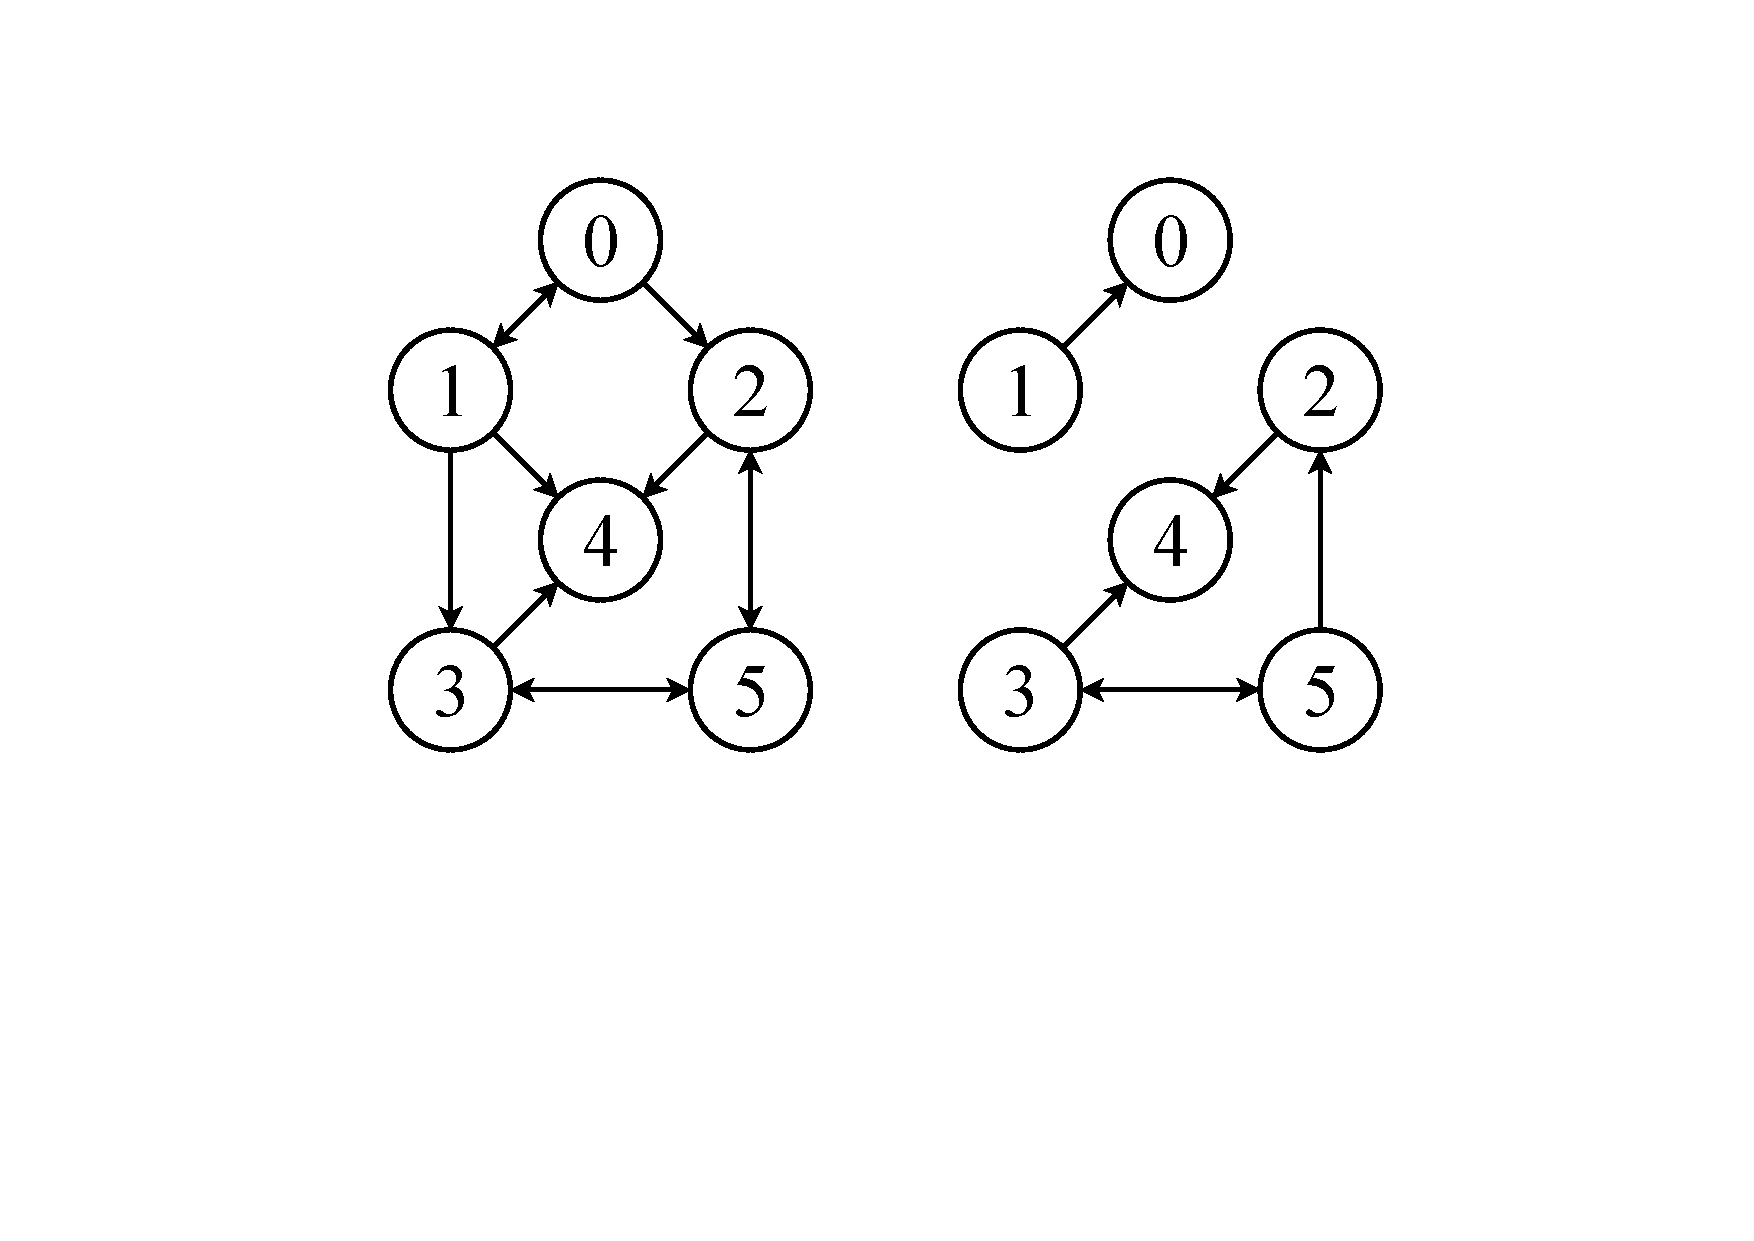
\includegraphics[scale=.3, clip, trim=180 230 440 80 ]{img/arte/graphs-BFS-F1.pdf}
    		
    		(a)
    	\end{minipage}
    	\begin{minipage}{0.45\textwidth}
    		\centering
    		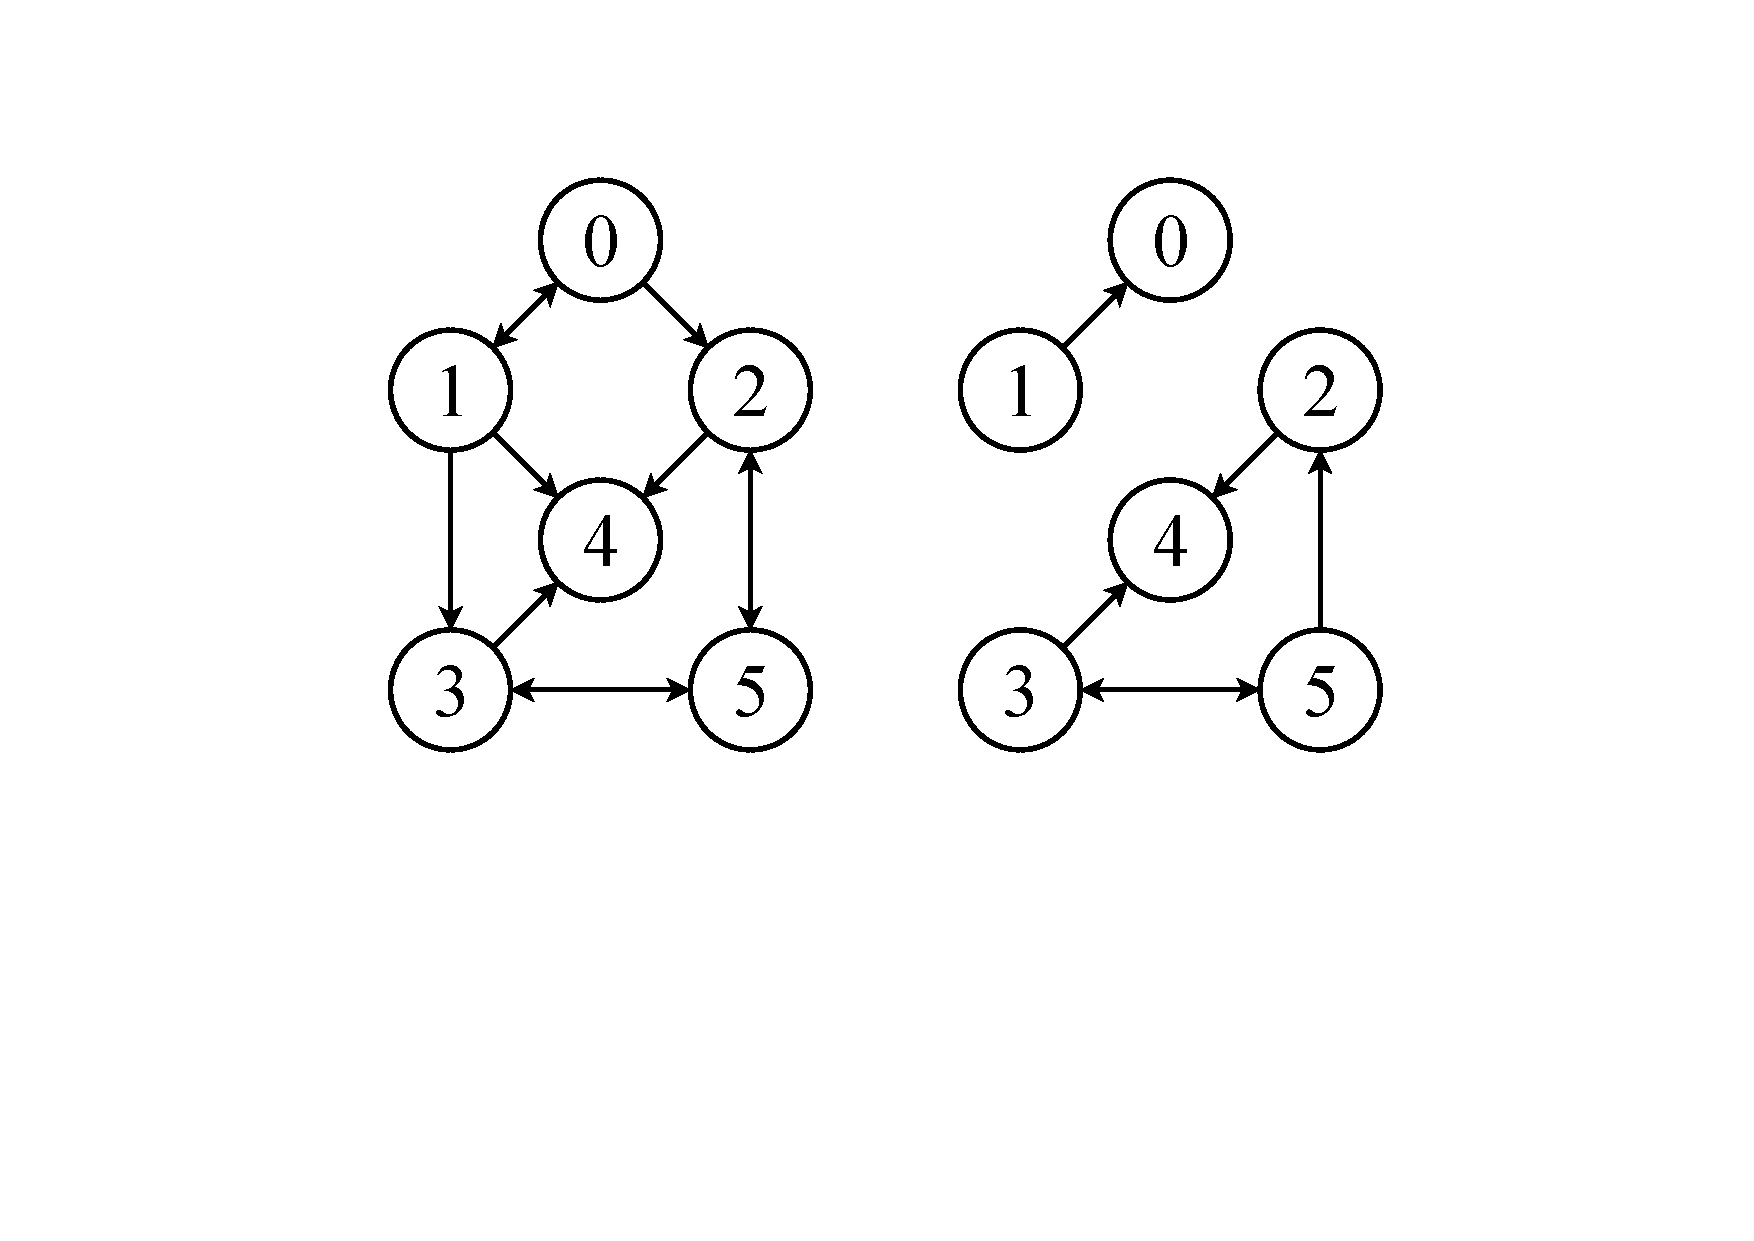
\includegraphics[scale=.3, clip, trim=450 230 170 80]{img/arte/graphs-BFS-F1.pdf}
    		
    		$T = \{2, 2, 1, 0, 0, 0\}$
    		
    		(b)
    	\end{minipage}

    \caption{Ejemplo de Fase 1 de BFS. (a) Índices asignados a los nodos. (b) Aristas restantes después de BFS, junto listado de recorrido $T$.}
    \label{fig:bfs1}
\end{figure}


Luego comprimen por separado trozos consecutivos de $l$ nodos, siendo $l$ un valor específico que define el nivel de compresión. Cada trozo comprimido $C$, conformado por los nodos $v_{i}, v_{i + 1}, ..., v_{i + l - 1}$, lleva prefijado la secuencia $\{k_{i}, k_{i + 1}, ..., k_{i + l - 1}\}$.

En la Fase 2, codifican la lista de adyacencia $A_{i}$ de cada nodo $v_{i} \in V$ de un trozo $C$ en orden creciente. Cada lista codificada consiste en la diferencia entre elementos adyacentes en la lista y un indicador tipo del set $\{\alpha, \beta, \chi, \phi\}$. Con $A_{i}^{j}$ indicando el elemento $j$ de la lista $A_{i}$, distinguen tres casos:

\begin{enumerate}
	\item $A_{i - 1}^{j} \leq A_{i}^{j - 1} < A_{i}^{j}$: el código es $\phi \cdot (A_{i}^{j} - A_{i}^{j - 1} - 1)$.
	\item $A_{i}^{j - 1} < A_{i - 1}^{j} \leq A_{i}^{j}$: el código es $\beta \cdot (A_{i}^{j} - A_{i - 1}^{j})$.
	\item $A_{i}^{j - 1} < A_{i}^{j} < A_{i - 1}^{j}$: se subdivide en dos subcasos:
	\begin{enumerate}
		\item Si $A_{i}^{j} - A_{i}^{j - 1} - 1 \leq A_{i - 1}^{j} - A_{i}^{j} - 1$: el código es $\alpha \cdot (A_{i}^{j} - A_{i}^{j - 1} - 1)$.
		\item De otro modo: el código es $\chi \cdot (A_{i - 1}^{j} - A_{i}^{j} - 1)$.
	\end{enumerate}
\end{enumerate}

Los tipo $\alpha$ y $\phi$ codifican la diferencia con respecto al elemento previo de la lista ($A_{i}^{j - 1}$), mientras $\beta$ y $\chi$ con respecto al elemento en la misma posición de la lista de adyacencia del nodo previo ($A_{i - 1}^{j}$). Cuando $A_{i - 1}^{j}$ no existe se reemplaza por $A_{k}^{j}$, donde $k (k < i - 1 \wedge v_{k} \in C)$ es el índice más cercano a $i$ para cual el grado de $v_{k}$ no es menor que $j$, o por un código tipo $\phi$ en caso que un nodo así no exista.

En la \autoref{table:bfs-adjacency} se ilustra un ejemplo de listado de adyacencia, y en la \autoref{table:bfs-coded} su codificación basada en los casos ya mencionados.

 \begin{table}%[b]
\caption{Lista de adyacencia para BFS, con $v_{i}$ siendo el primer nodo de un trozo.}
\label{table:bfs-adjacency}
\centering
\footnotesize

\begin{tabular}{|l|l|l|}
	\toprule
	Nodo & Grado & Adyacentes \\
	\midrule
	... & ... & ... \\
	i & 8 & 13, 15, 16, 17, 20, 21, 23, 24 \\
	i + 1 & 9 & 13, 15, 16, 17, 19, 20, 25, 31, 32 \\
	i + 2 & 0 &  \\
	i + 3 & 2 & 15, 16 \\
	... & ... & ... \\
\end{tabular}
\end{table} 


 \begin{table}%[b]
\caption{Codificación BFS del listado de adyacencia en la Tabla~\ref{table:bfs-adjacency}.}
\label{table:bfs-coded}
\centering
\footnotesize

\begin{tabular}{|l|l|l|}
	\toprule
	Nodo & Grado & Adyacentes \\
	\midrule
	... & ... & ... \\
	i & 8 & $\phi13$, $\phi1$, $\phi0$, $\phi0$, $\phi2$, $\phi0$, $\phi1$, $\phi0$ \\
	i + 1 & 9 & $\beta0$, $\beta0$, $\beta0$, $\beta0$, $\chi0$, $\alpha0$, $\beta2$, $\phi5$, $\phi0$ \\
	i + 2 & 0 &  \\
	i + 3 & 2 & $\beta2$, $\alpha0$ \\
	... & ... & ... \\
\end{tabular}
\end{table} 


Luego, aprovechan distintos tipos de redundancias en los listados de adyacencia, como se puede ver en la \autoref{table:bfs-exploting}, distinguiendo cuatro casos:

\begin{enumerate}
	\item Un conjunto de líneas idénticas (ver bloque ancho amarillo en la \autoref{table:bfs-exploting}) se codifican asignando un multiplicador a la primera línea de la secuencia.
	\item Los intervalos con grado constante de nodos (ver bloque consecutivo de 9s en la \autoref{table:bfs-exploting}), se codifican por su diferencia.
	\item Una secuencia de largo $\mathcal{L}_{min}$ de elementos idénticos (ver el bloque de $\phi1$s en la \autoref{table:bfs-exploting}), se codifica por su largo.
	\item Un bloque de filas idénticas (ver gran bloque azul en la \autoref{table:bfs-exploting}) que superen un umbral $\mathcal{A}_{min}$, se codifica por su largo.
\end{enumerate}

 \begin{table}%[b]
\caption{Ejemplo de redundancias a explotar en listado de adyacencia de BFS.}
\label{table:bfs-exploting}
\centering
\footnotesize

\begin{tabular}{|l|llllllllll|}
	\toprule
	Grado & \multicolumn{9}{l}{Adyacentes} & \\
	\midrule
	\cellcolor{blanco} ... & \multicolumn{9}{l}{\cellcolor{blanco} ...} & \\
	\cellcolor{blanco} 0 & \multicolumn{9}{l}{} & \\
	\cellcolor{rojo} 9 & \cellcolor{blanco} $\beta1,$ & \cellcolor{cafe} $\phi1,$ & \cellcolor{cafe} $\phi1,$ & \cellcolor{cafe} $\phi1,$ & \cellcolor{blanco} $\phi0,$ & \cellcolor{blanco} $\phi1,$ & \cellcolor{blanco} $\phi1,$ & \cellcolor{blanco} $\phi1,$ & \cellcolor{blanco} $\phi1,$ & \\
    \cellcolor{rojo} 9 & \cellcolor{azul} $\beta0,$ & \cellcolor{azul} $\beta1,$ & \cellcolor{azul} $\beta0,$ & \cellcolor{azul} $\beta0,$ & \cellcolor{azul} $\beta0,$ & \cellcolor{azul} $\beta0,$ & \cellcolor{azul} $\beta0,$ & \cellcolor{azul} $\beta0,$ & \cellcolor{blanco} $\beta2,$ & \\
    \cellcolor{blanco} 10 &  \cellcolor{azul} $\beta0,$ & \cellcolor{azul} $\beta1,$ & \cellcolor{azul} $\beta0,$ & \cellcolor{azul} $\beta0,$ & \cellcolor{azul} $\beta0,$ & \cellcolor{azul} $\beta0,$ & \cellcolor{azul} $\beta0,$ & \cellcolor{azul} $\beta0,$  & \cellcolor{blanco} $\beta1,$ & \cellcolor{blanco} $\phi903$ \\
    \cellcolor{blanco} 10 &  \cellcolor{azul} $\beta0,$ & \cellcolor{azul} $\beta1,$ & \cellcolor{azul} $\beta0,$ & \cellcolor{azul} $\beta0,$ & \cellcolor{azul} $\beta0,$ & \cellcolor{azul} $\beta0,$ & \cellcolor{azul} $\beta0,$ & \cellcolor{azul} $\beta0,$  & \cellcolor{blanco} $\beta223,$ & \cellcolor{blanco} $\phi900$ \\
    \cellcolor{blanco} 10 &  \cellcolor{azul} $\beta0,$ & \cellcolor{azul} $\beta1,$ & \cellcolor{azul} $\beta0,$ & \cellcolor{azul} $\beta0,$ & \cellcolor{azul} $\beta0,$ & \cellcolor{azul} $\beta0,$ & \cellcolor{azul} $\beta0,$ & \cellcolor{azul} $\beta0,$  & \cellcolor{blanco} $\beta1,$ & \cellcolor{blanco} $\alpha0$ \\
    \cellcolor{amarillo} 10 & \cellcolor{verde} $\beta0,$ & \cellcolor{verde} $\beta1,$ & \cellcolor{verde} $\beta0,$ & \cellcolor{verde} $\beta0,$ & \cellcolor{verde} $\beta0,$ & \cellcolor{verde} $\beta0,$ & \cellcolor{verde} $\beta0,$ & \cellcolor{verde} $\beta0,$ & \cellcolor{amarillo} $\beta1,$ & \cellcolor{amarillo} $\beta0$ \\
    \cellcolor{amarillo} 10 & \cellcolor{verde} $\beta0,$ & \cellcolor{verde} $\beta1,$ & \cellcolor{verde} $\beta0,$ & \cellcolor{verde} $\beta0,$ & \cellcolor{verde} $\beta0,$ & \cellcolor{verde} $\beta0,$ & \cellcolor{verde} $\beta0,$ & \cellcolor{verde} $\beta0,$ & \cellcolor{amarillo} $\beta1,$ & \cellcolor{amarillo} $\beta0$ \\
    \cellcolor{amarillo} 10 & \cellcolor{verde} $\beta0,$ & \cellcolor{verde} $\beta1,$ & \cellcolor{verde} $\beta0,$ & \cellcolor{verde} $\beta0,$ & \cellcolor{verde} $\beta0,$ & \cellcolor{verde} $\beta0,$ & \cellcolor{verde} $\beta0,$ & \cellcolor{verde} $\beta0,$ & \cellcolor{amarillo} $\beta1,$ & \cellcolor{amarillo} $\beta0$ \\
    \cellcolor{amarillo} 10 & \cellcolor{verde} $\beta0,$ & \cellcolor{verde} $\beta1,$ & \cellcolor{verde} $\beta0,$ & \cellcolor{verde} $\beta0,$ & \cellcolor{verde} $\beta0,$ & \cellcolor{verde} $\beta0,$ & \cellcolor{verde} $\beta0,$ & \cellcolor{verde} $\beta0,$ & \cellcolor{amarillo} $\beta1,$ & \cellcolor{amarillo} $\beta0$ \\
    \cellcolor{blanco} 10 &  \cellcolor{azul} $\beta0,$ & \cellcolor{azul} $\beta1,$ & \cellcolor{azul} $\beta0,$ & \cellcolor{azul} $\beta0,$ & \cellcolor{azul} $\beta0,$ & \cellcolor{azul} $\beta0,$ & \cellcolor{azul} $\beta0,$ & \cellcolor{azul} $\beta0,$  & \cellcolor{blanco} $\alpha76,$ & \cellcolor{blanco} $\alpha232$ \\
    \cellcolor{blanco} 9 &  \cellcolor{azul} $\beta0,$ & \cellcolor{azul} $\beta1,$ & \cellcolor{azul} $\beta0,$ & \cellcolor{azul} $\beta0,$ & \cellcolor{azul} $\beta0,$ & \cellcolor{azul} $\beta0,$ & \cellcolor{azul} $\beta0,$ & \cellcolor{azul} $\beta0,$  & \cellcolor{blanco} $\beta0$ & \\
	\cellcolor{blanco} ... & \multicolumn{9}{l}{\cellcolor{blanco} ...} & \\
\end{tabular}
\end{table} 


Para ello introducen un nuevo símbolo $\Sigma$, seguido de un indicador $\Sigma_{F}$ toma valor 2 si la redundancia es de tipo 3, 3 si es de tipo 4, o 1 si son ambas. Dependiendo de la redundancia a codificar, el código se expresa como `$tipo\:\Sigma\:\Sigma_{F}\:gap\:l$'  o `$tipo\:\Sigma\:\Sigma_{F}\:gap\:l\:w\:h$', siendo $tipo$ uno de los símbolos del set $\{\alpha, \beta, \chi, \phi\}$, $gap$ un entero indicando la diferencia, $l$ la cantidad de elementos idénticos en la misma línea, $w$ y $h$ el ancho y alto de las columnas y filas idénticas. En la \autoref{table:bfs-exploted} se ilustra esta codificación para el caso ejemplo de la \autoref{table:bfs-exploting}.

 \begin{table}%[b]
\caption{Ejemplo de redundancias codificadas de BFS para la Tabla~\ref{table:bfs-exploting}.}
\label{table:bfs-exploted}
\centering
\footnotesize

\begin{tabular}{|l|l|llll|}
	\toprule
	Líneas & Grado & \multicolumn{3}{l}{Enlaces} &  \\
	\midrule
	... & ... & ... & & &  \\
	0 & 0 & & & & \\
	0 & 9 & $\beta7$, & $\phi\:\Sigma\:2\:1\:1$, & $\phi0$, & $\phi\:\Sigma\:2\:1\:2$ \\
	0 & 0 & $\beta\:\Sigma\:3\:0\:7\:5$, & $\beta1$, & $\beta\:\Sigma\:2\:0\:4$, & $\beta2$ \\
	0 & 1 & $\beta1$, & $\phi903$ & & \\
	0 & 0 & $\beta223$, & $\phi900$ & & \\
	0 & 0 & $\beta1$, & $\alpha0$ & & \\
	3 & 0 & $\beta1$, & $\beta0$ & & \\
	0 & 0 & $\alpha76$, & $\alpha232$ & & \\
	0 & -1 & $\beta0$ & & & \\
	... & ... & ... & & &  \\
\end{tabular}
\end{table} 


Finalmente, usan códigos Huffman para codificar $\alpha, \beta, \chi, \phi$, y proponen una nueva codificación $\pi$ para cifrar diferencias, $\Sigma$, y otros enteros.

\textcolor{red}{¿Es muy extendida esta explicación? Quizás podría detallar el método un poco menos.}


\subsection{Using Re-Pair, \textit{Claude y Navarro}}
El trabajo de Claude y Navarro \cite{claude2010fast} propone usar Re-Pair \cite{larsson2000off}, un método de compresión basado en gramática, para comprimir grafos dirigidos como el grafo de la Web. Re-Pair consiste en buscar el par de símbolos más frecuente en una secuencia y reemplazar cada ocurrencia por un nuevo símbolo, el cual se añade a un diccionario como nueva regla. En la \autoref{table:repair} se muestra un ejemplo simple de Re-Pair, donde las reglas conforman el diccionario para descomprimir la secuencia.

 \begin{table}%[b]
\caption{Ejemplo de Re-Pair. Las reglas en la tabla conforman el diccionario asociado a la compresión.}
\label{table:repair}
\centering
\small

\begin{tabular}{|l|l|}
	\toprule
	Reglas & String \\
	\midrule
	 & $singing.do.wah.diddy.diddy.dum.diddy.do$ \\
	$A \rightarrow .d$ & $singingAo.wahAiddyAiddyAumAiddyAo$ \\
	$B \rightarrow dd$ & $singingAo.wahAiByAiByAumAiByAo$ \\
	$C \rightarrow Ai$ & $singingAo.wahCByCByAumCByAo$ \\
	$D \rightarrow By$ & $singingAo.wahCDCDAumCDAo$ \\
	$E \rightarrow CD$ & $singingAo.wahEEAumEAo$ \\
	$F \rightarrow in$ & $sFgFgAo.wahEEAumEAo$ \\
	$G \rightarrow Ao$ & $sFgFgG.wahEEAumEG$ \\
	$H \rightarrow Fg$ & $sHHG.wahEEAumEG$ \\
	\bottomrule
\end{tabular}
\end{table} 


Claude y Navarro \cite{claude2010fast} aplican esta idea a los listados de adyacencia de un grafo dirigido. Si $V = \{v_{1}, v_{1}, ..., v_{n}\}$ es el listado de $n$ nodos del grafo $G$, $adj(v_{i}) = \{v_{i,1}, v_{i,2},... , v_{i,a_{i}}\}$ el listado de $a_{i}$ nodos adyacentes a $v_{i}$, y $\overline{v_{i}}$ una alternativa de notación para el nodo $v_{i}$, proponen concatenar todos los listados de adyacencia con la siguiente notación:

\begin{equation} \label{eq:RepairGrafo}
	T = T(G) = \overline{v_{1}} \; v_{1,1}, v_{1,2}, ..., v_{1,a_{1}}, \overline{v_{2}} \; v_{2,1}, v_{2,2}, ..., v_{2,a_{2}}, ..., \overline{v_{n}} \; v_{n,1}, v_{n,2}, ..., v_{n,a_{n}}
\end{equation}

\noindent donde se debe cumplir con $v_{i,j} < v_{i, j+1}$ para cualquier $1 \leq i \leq n$ y $1 \leq j \leq a_{i}$. Esto significa que cada lista de adyacencia concatenada debe partir con su nodo referencia, y todos los nodos de ella deben estar ordenados de menor a mayor. Luego se van reemplazando recursivamente, sin incluir los nodos de referencia, los pares de símbolos consecutivos más frecuentes por uno nuevo, hasta que no sea conveniente, y cada reemplazo se guarda como regla. 

Finalmente, se eliminan los nodos de referencia con el cuidado de codificar en dos bitmaps: En $B1$ si tienen nodos adyacentes, y en $B2$ la ubicación de dichos nodos en el arreglo final. En la \autoref{fig:repairCN} se ilustra un ejemplo, donde en (a) se tiene el grafo de ejemplo, en (b) la concatenación $T(G)$ de todos los listados de adyacencia ordenados de menor a mayor, los reemplazos necesarios para su compresión y el arreglo resultante, y en (c) los bitmaps indicadores de los nodos de referencia. Se debe notar que la notación alternativa $\overline{v_{i}}$ se reemplaza por $-v_{i}$ en el arreglo. También presentan otras mejoras, como usar diferencias para codificar los listados de adyacencia o re-ordenar los nodos para aprovechar mejor Re-Pair.

\begin{figure}%[b]
    	\centering
    	\begin{minipage}{1\textwidth}
    		\begin{minipage}{.6\textwidth}
    			\centering
    			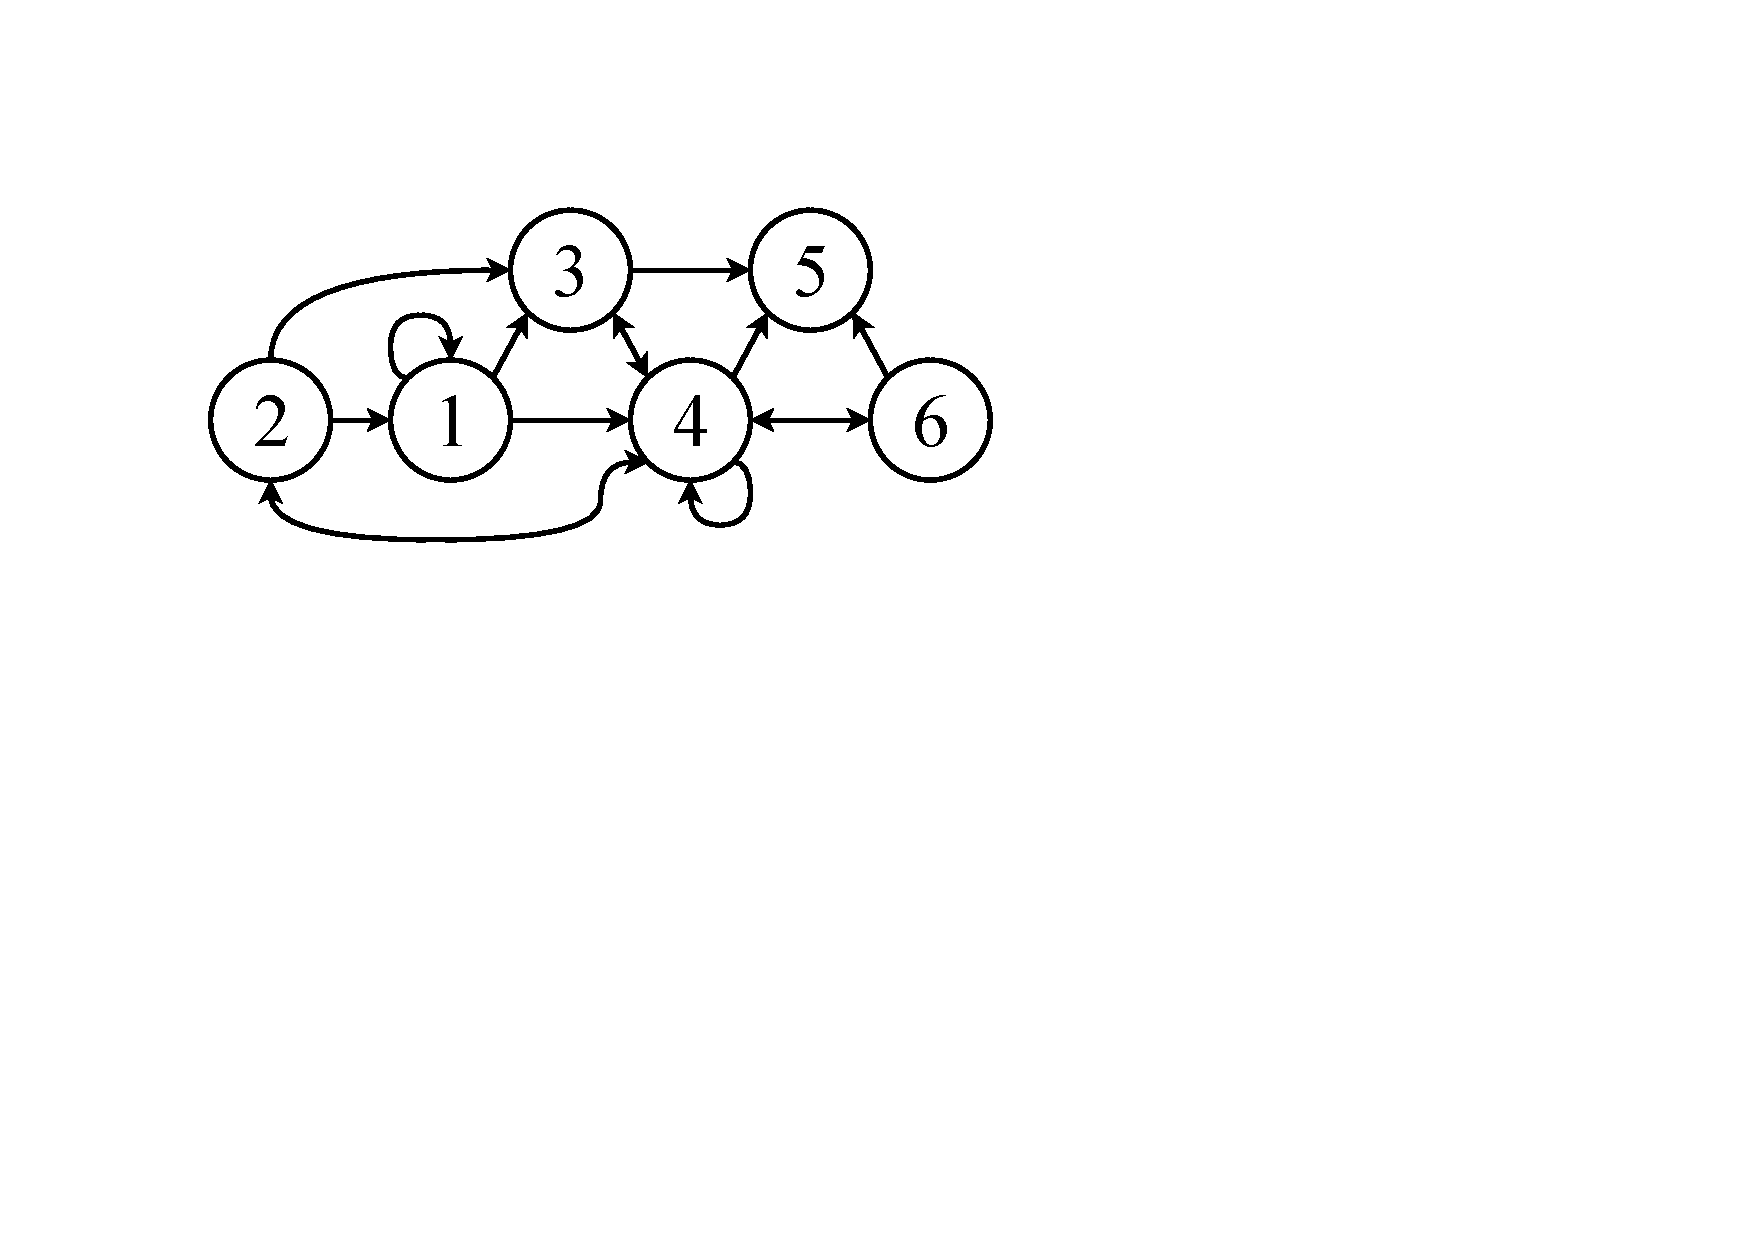
\includegraphics[scale=.3, clip,  trim=90 330 350 90]{img/arte/graphs-repair.pdf}
    		
    			(a)
    		\end{minipage}
    		\begin{minipage}{.35\textwidth}
    			\centering
    			\vspace{5mm}
		    	\begin{tabular}{|l|l|}
		    		\hline
		    		B1 & 111101 \\
		    		\hline
		    		B2 & 1111001\\
		    		\hline
		    	\end{tabular}
		    	\vspace{5mm}
		    	
    			(c)
    		\end{minipage}
    	\end{minipage}
    	\vspace{5mm}
    	
    	\begin{minipage}{1\textwidth}
    		\centering

		\begin{tabular}{l||l|l|l|l|l|l|l|l|l|l|l|l|l|l|l|l|l|l|l|l|l|}
			\toprule
			$T(G)$ & -1 & 1 & 3 & 4 & -2 & 1 & 3 & 4 & -3 & 4 & 5 & -4 & 3 & 4 & 5 & 6 & -5 & -6 & 4 & 5 \\
			\midrule
			$7 \rightarrow 4 \; 5$ & -1 & 1 & 3 & 4 & -2 & 1 & 3 & 4 & -3 & 7 & -4 & 3 & 7 & 6 & -5 & -6 & 7 \\
			\cline{1-18}
			$8 \rightarrow 1 \; 3$ & -1 & 8 & 4 & -2 & 8 & 4 & -3 & 7 & -4 & 3 & 7 & 6 & -5 & -6 & 7 \\
			\cline{1-16}
			$9 \rightarrow 8 \; 4$ & -1 & 9 & -2 & 9 & -3 & 7 & -4 & 3 & 7 & 6 & -5 & -6 & 7 \\
			\cline{1-14}
			Borrar $<0$ & 9 & 9 & 7 & 3 & 7 & 6 & 7 \\
			\cline{1-8}
		\end{tabular}				
		\vspace{5mm}
		
		(b)
    	\end{minipage}

    \caption{Ejemplo para Re-Pair aplicado a grafos por Claude y Navarro. (a) Grafo de ejemplo. (b) Listado concatenado $T(G)$ y resultado final luego de tres reemplazos y eliminar nodos de referencia. (c) Bitmaps indicadores de nodos de referencia removidos.}
    \label{fig:repairCN}
\end{figure}


Una propuesta de compresión más reciente, de Maneth y Peternek \cite{maneth2016compressing}, también generaliza Re-Pair para comprimir grafos, específicamente hipergrafos dirigidos.


\subsection{Virtual Node Mining, \textit{Buehrer y Chellapilla}}
Buehrer y Chellapilla \cite{BuehrerChellapilla} aprovechan que muchos grupos de nodos en el grafo de la Web consisten en conjuntos de sitios que comparten los mismos vecinos directos, lo que genera un grafo bipartito completo. Su propuesta reduce la cantidad de aristas en grafos dirigidos, definiendo nodos virtuales que son agregados artificialmente al grafo entre los dos conjuntos del biclique. Esto reduce la cantidad total de aristas, ya que cada biclique une un set de $U$ nodos con uno de $W$ nodos, genera en total $|U \times W|$ aristas, y usando un nodo virtual disminuye a $|U + W|$, un gran ahorro cuando los bicliques son grandes. En la \autoref{fig:virtualNode} se ejemplifica este reemplazo, cambiando de las iniciales 30 aristas del biclique en (a), 19 por un nodo virtual VN en (b), quedando solo 11 aristas restantes.

\begin{figure}%[b]
    	\centering
    	\begin{minipage}{0.45\textwidth}
    		\centering
    		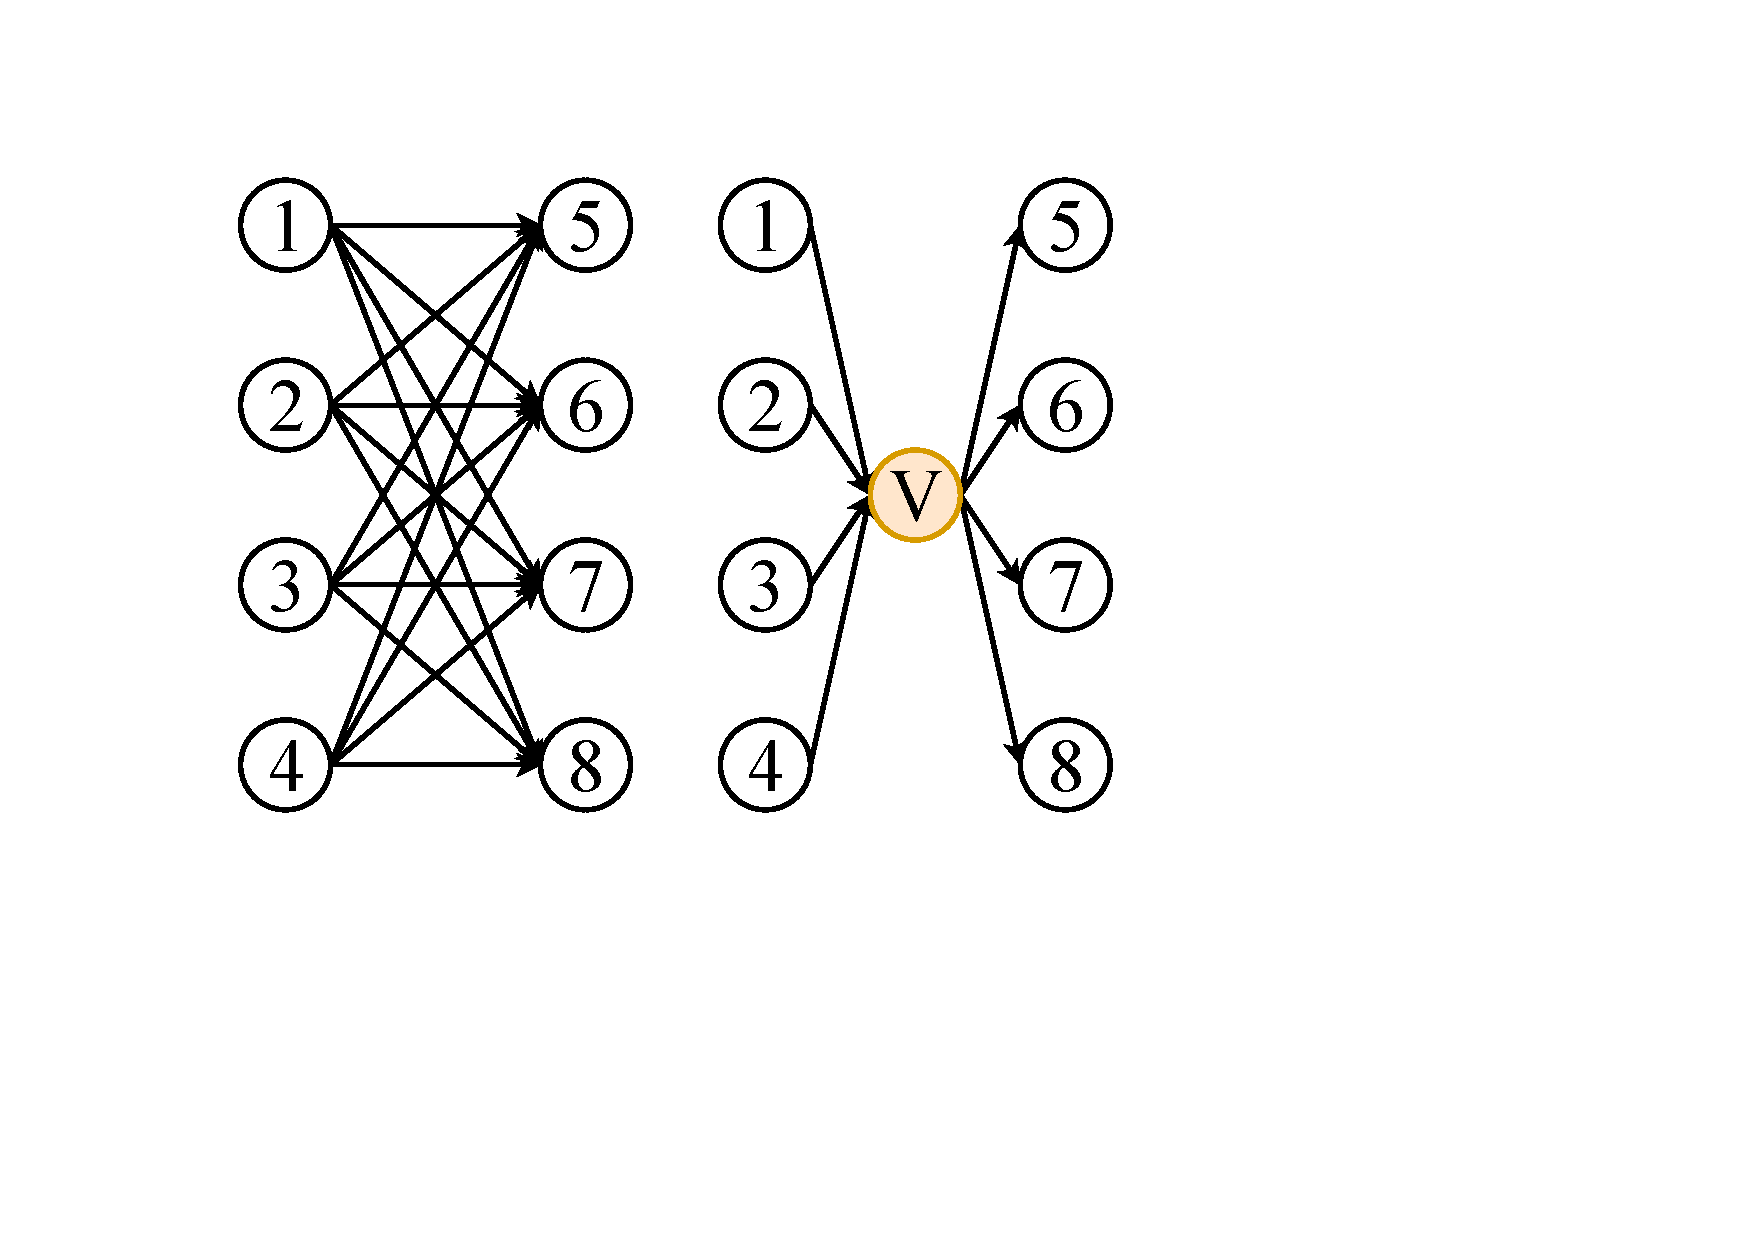
\includegraphics[scale=.3, clip,  trim=100 200 520 70]{img/arte/graphs-virtualNode.pdf}
    		
    		(a)
    	\end{minipage}
    	\begin{minipage}{0.45\textwidth}
    		\centering
    		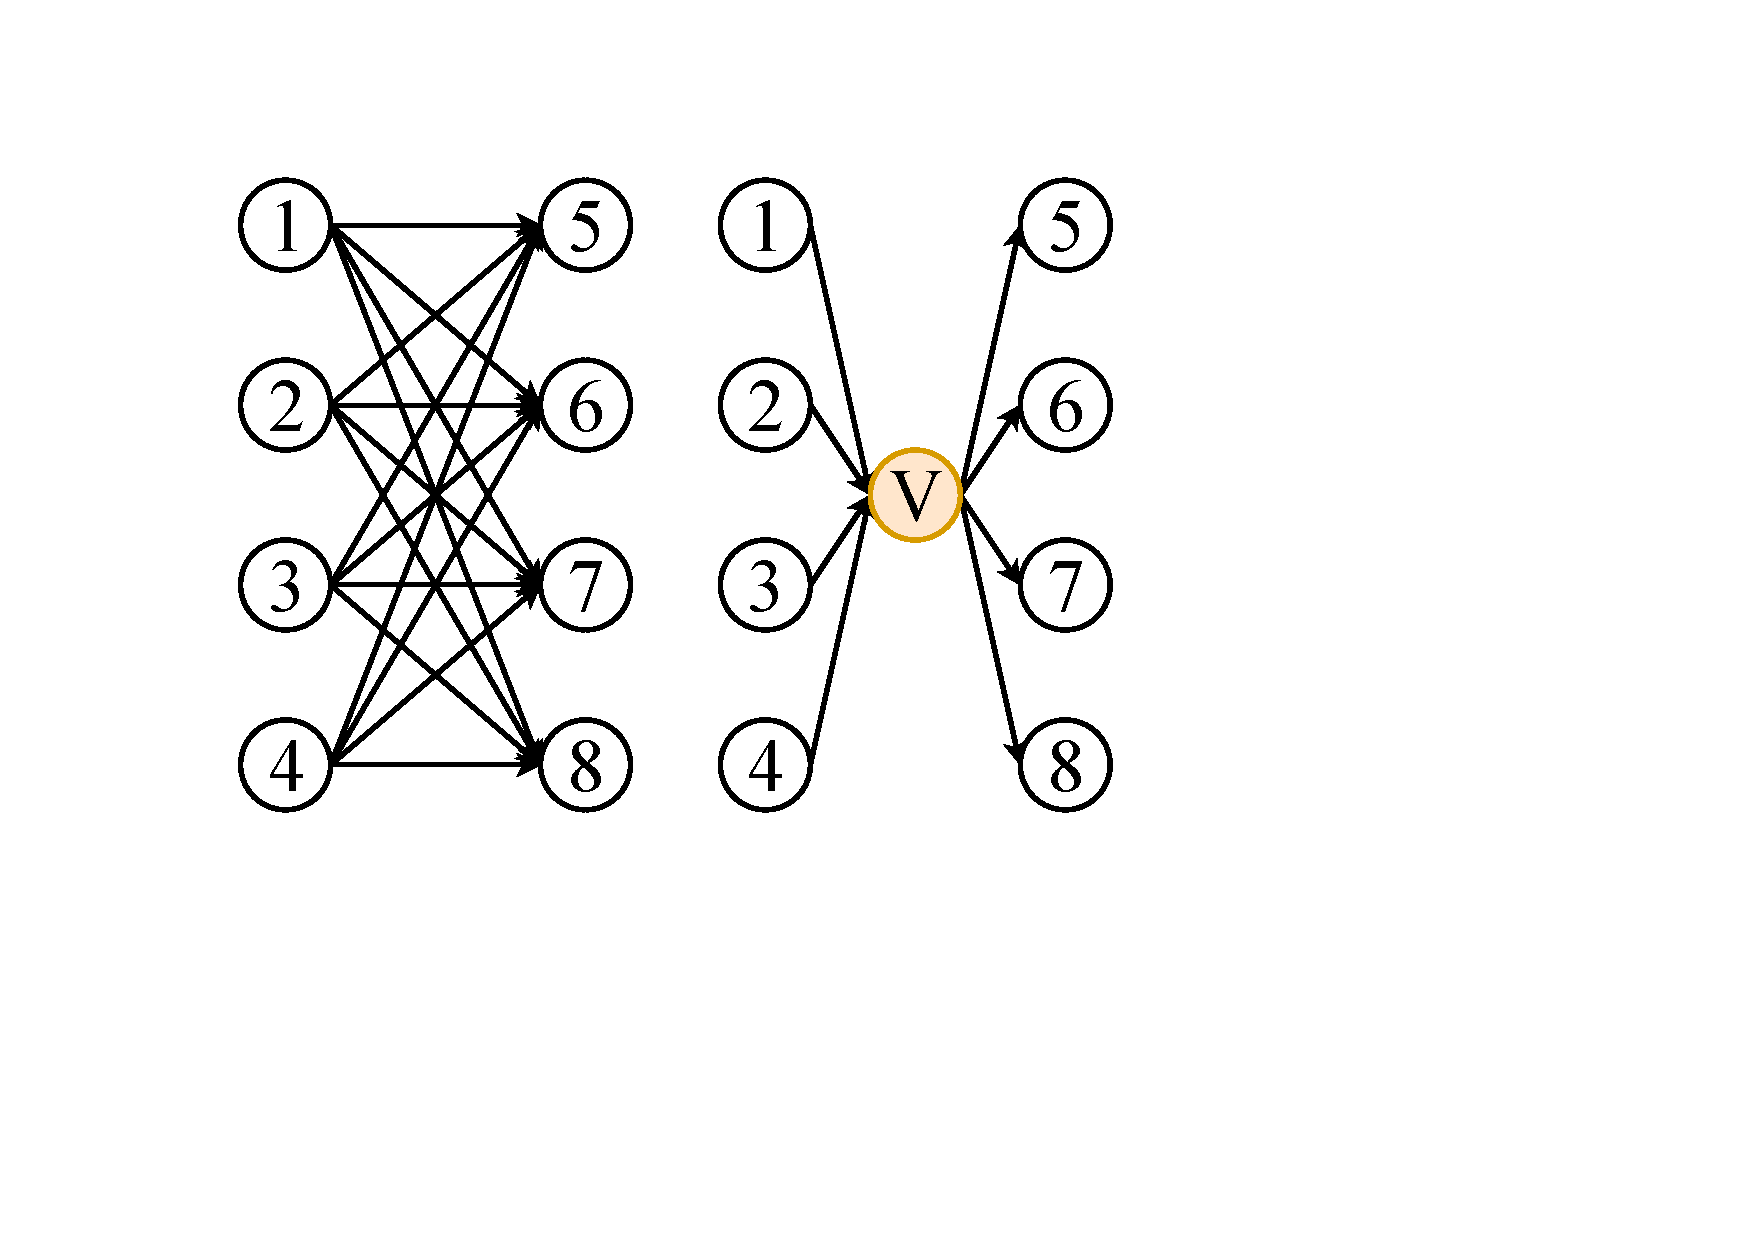
\includegraphics[scale=.3, clip, trim=330 200 290 70]{img/arte/graphs-virtualNode.pdf}
    		
    		(b)
    	\end{minipage}

    \caption{Ejemplo de reemplazo por nodo virtual. (a) Biclique. (b) Biclique con reemplazo de aristas por nodo virtual $V$.}
    \label{fig:virtualNode}
\end{figure}


Este proceso se repite iterativamente hasta que ya no se reducen significativamente más aristas. Luego aplican codificación delta (ver \autoref{sec:Ucoding}) sobre el grafo reducido. La propuesta logra una buena compresión, pero no reportan los tiempos de acceso. Además, su resultado no se ve afectado por el orden de numeración de los nodos, y permite actualizaciones.

Anh y Moffat \cite{anh2010local} también aprovechan esta localidad y similaridad en los listados de adyacencia, dividiendo en grupos de $h$ listas consecutivas. Luego reducen las listas aplicando reglas gramáticas como Re-Pair \cite{larsson2000off} de manera recursiva, y finalmente aplican codificaciones como el código $\zeta$ \cite{boldi2005codes}.


\subsection{k2-tree, \textit{Brisaboa, Ladra y Navarro}}
Una propuesta que aprovecha lo dispersa y agrupada que es la matriz de adyacencia del grafo de la Web es la propuesta por Brisaboa, Ladra y Navarro \cite{brisaboa2009k} donde proponen una estructura llamada k2-tree para ahorrar espacio y poder responder consultas tanto de vecinos directos como reversos. Esto último significa que este método, si bien fue pensado para grafos dirigidos, también se puede aplicar para no dirigidos. En un trabajo posterior, lograron mejorar sus resultados aplicando el ordenamiento por BFS antes de crear su estructura \cite{brisaboa2014compact}.

Este modelo propone representar la matriz de adyacencia con un árbol $k_{2}$-nario de altura $h=\lceil(\log_k n)\rceil$, donde $n$ es el número de vértices en el grafo. Luego subdivide la matriz de adyacencia en $k^2$ submatrices de tamaño $n^{2}/k^{2}$, si una de ellas contiene solo ceros se representa solo con un bit en $0$, de lo contrario se marcan con un $1$ y se vuelven a subdividir de manera recursiva. Esta estructura soporta las consultas de vecinos directos y reversos de manera simétrica, ya que significa revisar las filas o columnas de la matriz. En la \autoref{fig:k2tree} se presenta (a) un ejemplo de una matriz de adyacencia y sus subdivisiones para k2tree, y (b) un diagrama de la estructura final.

\begin{figure}%[b]
    	\centering
    	\begin{minipage}{0.45\textwidth}
    		\centering
    		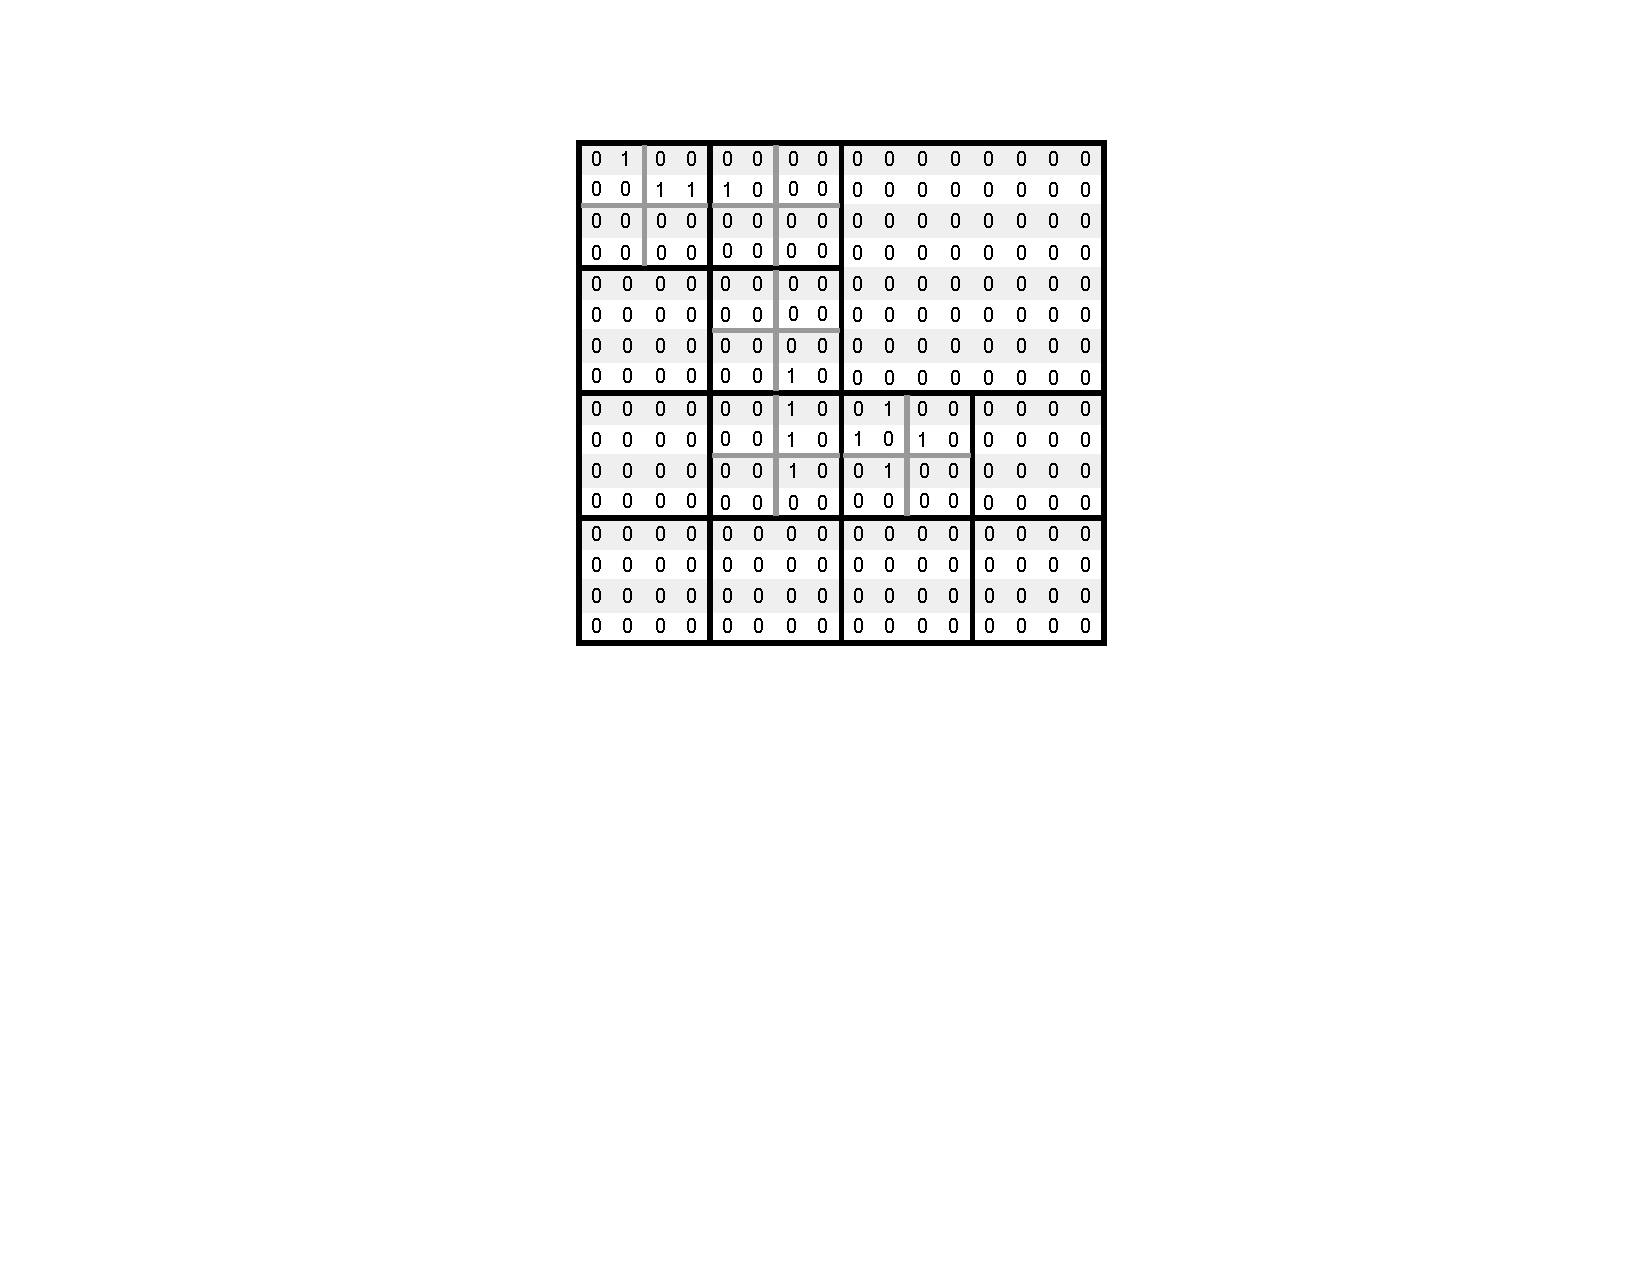
\includegraphics[scale=.6, clip,  trim=270 280 250 0]{img/arte/k2-tree-matrix.pdf}
    		
    		(a)
    	\end{minipage}
    	\begin{minipage}{0.45\textwidth}
    		\centering
    		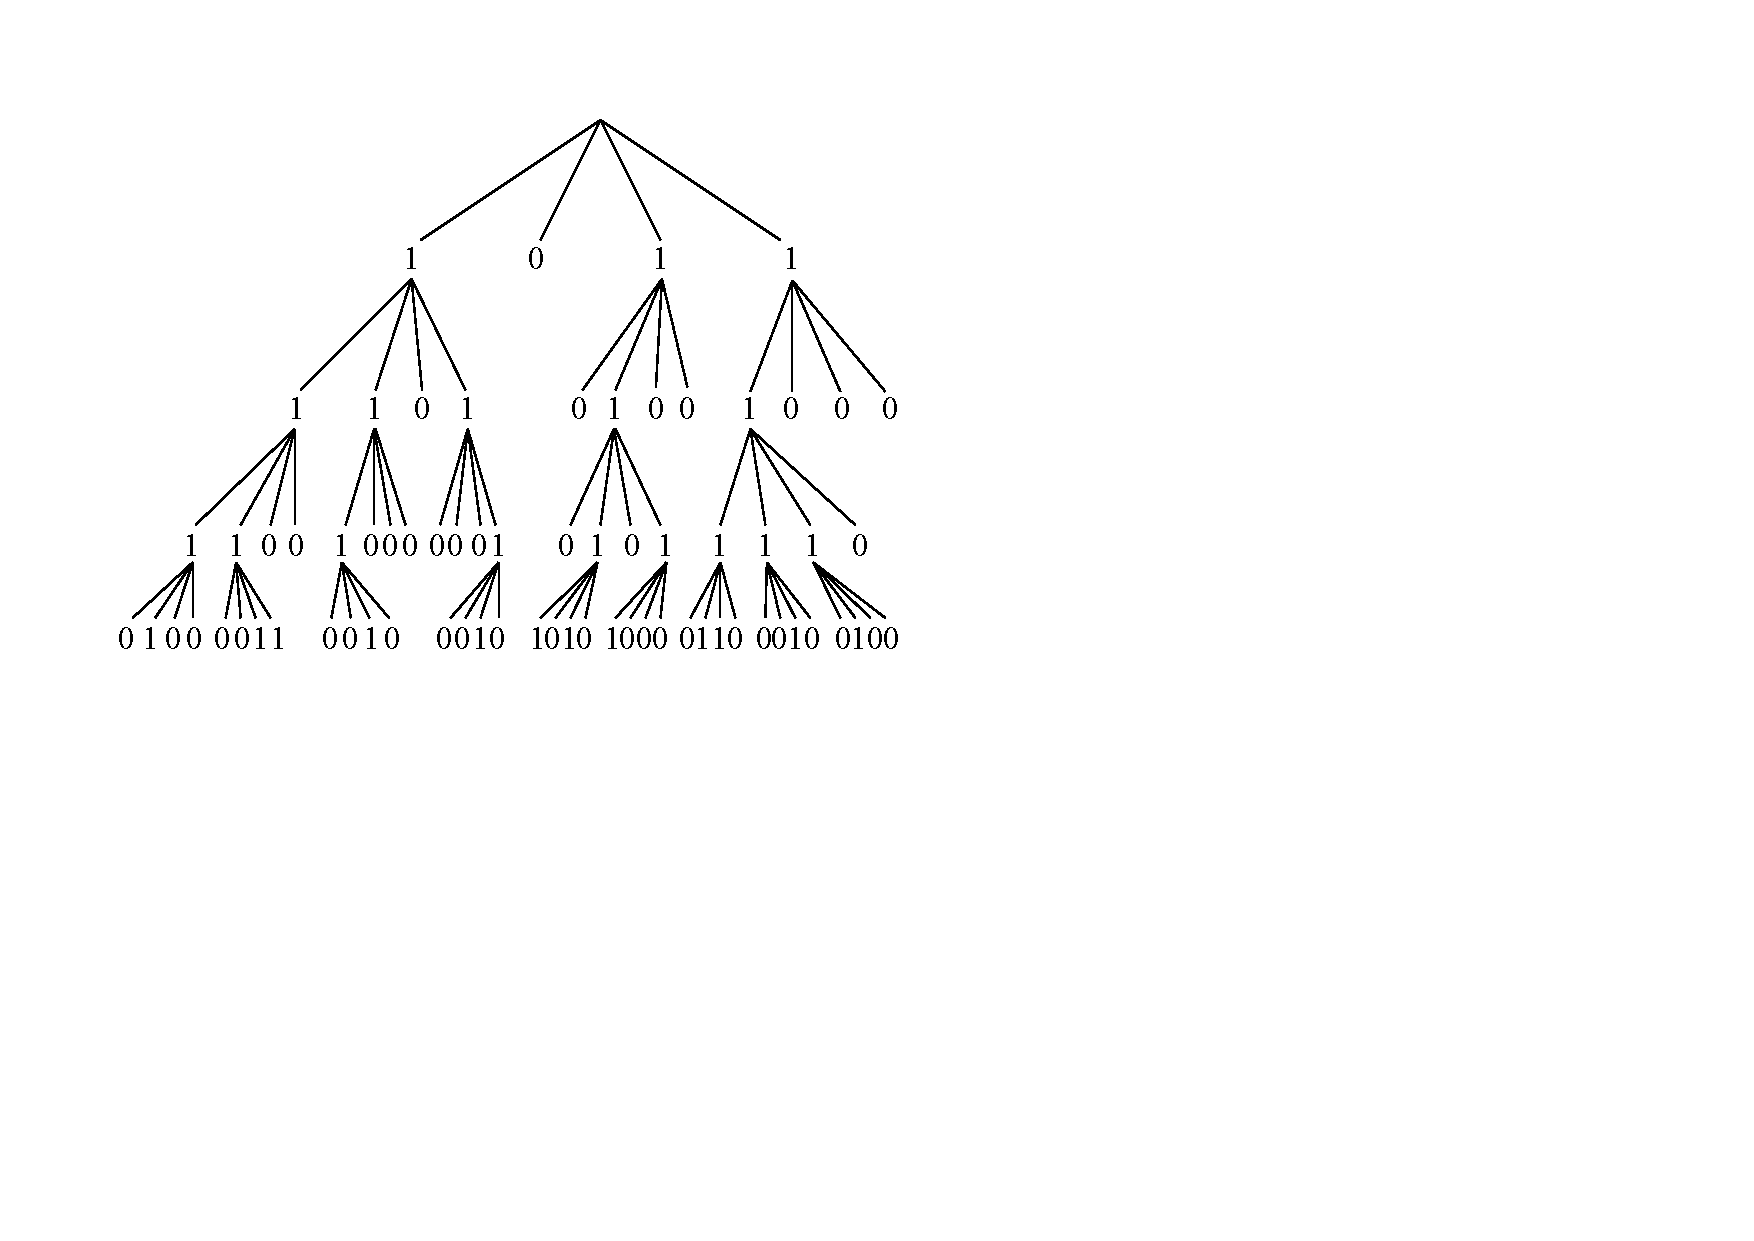
\includegraphics[scale=.5, clip, trim=50 280 410 0]{img/arte/graphs-k2tree.pdf}
    		
    		(b)
    	\end{minipage}

    \caption{Ejemplo de k2-tree. (a) Matriz de adyacencia. (b) Diagrama de estructura.}
    \label{fig:k2tree}
\end{figure}


Finalmente, la compresión se realiza representando el árbol usando dos arreglos de bits, un bitmap $T$ para representar la estructura del árbol, y un bitmap $L$ para representar las hojas, que representan las celdas de la matriz. Además usan un bitmap adicional para acelerar la resolución de consultas. 

En 2011, Hernández y Navarro \cite{hernandez2011compression} propusieron combinar varios métodos: Primero reducir la cantidad de aristas con nodos virtuales \cite{BuehrerChellapilla},  y luego comprimir usando la propuestas de k2-tree~\cite{brisaboa2009k}. Con esto, el número de aristas del grafo original se reduce cerca de diez veces, y el número de vértices aumenta en un $10\%$. Este enfoque proporciona resultados competitivos principalmente en grafos de la Web, pero no en grafos de redes sociales.

En trabajos posteriores, Hernandez y Navarro \cite{hernandez2012compressed, hernandez2014compressed} proponen una estructura bastante similar, que consiste en obtener subgrafos bipartitos de grafos dirigidos, o no dirigidos con aristas duplicadas, usando una heurística de cantidad de aristas a representar. Luego se obtiene un conjunto de subgrafos bipartitos y un grafo restante. Finalmente se construye una estructura compacta, basada en wavelet trees y bitmaps comprimidos para representar la colección de subgrafos, y el resto del grado se comprime con otras técnicas como k2tree~\cite{brisaboa2009k}. Esta estructura permite obtener los vecinos directos y reversos de grafos dirigidos, o grafos no dirigidos representados como dirigidos.


\subsection{List Merging, \textit{Grabowski y Bieniecki}}
Grabowski y Bieniecki~\cite{grabowski2014tight} proponen agrupar los listados de adyacencia de grafos dirigidos en bloques de $h$ listas cada uno, de manera similar a lo propuesto por Anh y Moffat~\cite{anh2010local}. Cada bloque luego es descompuesto en dos arreglos: el primero es \textit{long list}, un arreglo de todos los índices de los vértices presentes en el bloque de listados de adyacencia, sin repetir ninguno. El segundo es \textit{flags}, un arreglo de bits que permite la reconstrucción de las listas agrupadas. 

El arreglo de enteros \textit{long list} es reducido usando las diferencias, terminada en cero y codificada en bytes. El arreglo de bits \textit{flags} indica la pertenencia de los índices en \textit{long list} a sus listas de adyacencias asociadas. El número de bits por cada índice es $h$, definido como un múltiplo de 8. su largo queda definido por el largo de \textit{long list}. Este arreglo puede no comprimirse (en cual caso lo llaman \textit{LM-bitmap}), o codificarse usando las diferencias entre los 1 sucesivos, escritas en bytes individuales (\textit{LM-diff}).

Ambas secuencias, \textit{long list} y ya sea \textit{LM-bitmap} o \textit{LM-diff}, luego son concatenadas y comprimidas usando el algoritmo \textit{Deflate}. Este algoritmo consiste en una serie de bloques, todos precedidos por una cabecera de 3 bits, que indican lo siguiente:

\begin{itemize}
	\item Primer bit:
	\begin{itemize}
		\item 0: No es el último bloque de la secuencia.
		\item 1: Es el último bloque de la secuencia.
	\end{itemize}
	\item Segundo y tercer bit:
	\begin{itemize}
		\item 00: Bloque sin codificar.
		\item 01: Bloque codificado con Huffman, con un árbol de Huffman ya definido.
		\item 10: Bloque codificado con Huffman y su árbol asociado.
		\item 11: Reservado; No usar.
	\end{itemize}
\end{itemize}

Para más detalles sobre la codificación Huffman, ver la \autoref{sec:huffman}.


\subsection{GLOUDS, \textit{Fischer y Peters}}
Fischer y Peters \cite{fischer2016glouds} proponen una nueva estructura de datos sucintos para comprimir grafos dirigidos con forma de árbol, llamada \textit{GLOUDS (Graph Level Order Unary Degree Sequence)}. La idea del algoritmo es representar mediante otra estructura de datos sucintos para árboles de expansión, llamada \textit{LOUDS (Level Order Unary Degree Sequence)} \cite{jacobson1989space}, y agregarle información adicional para los nodos extra.

\begin{figure}%[b]
    	\centering
    	\begin{minipage}{0.25\textwidth}
    		\centering
    		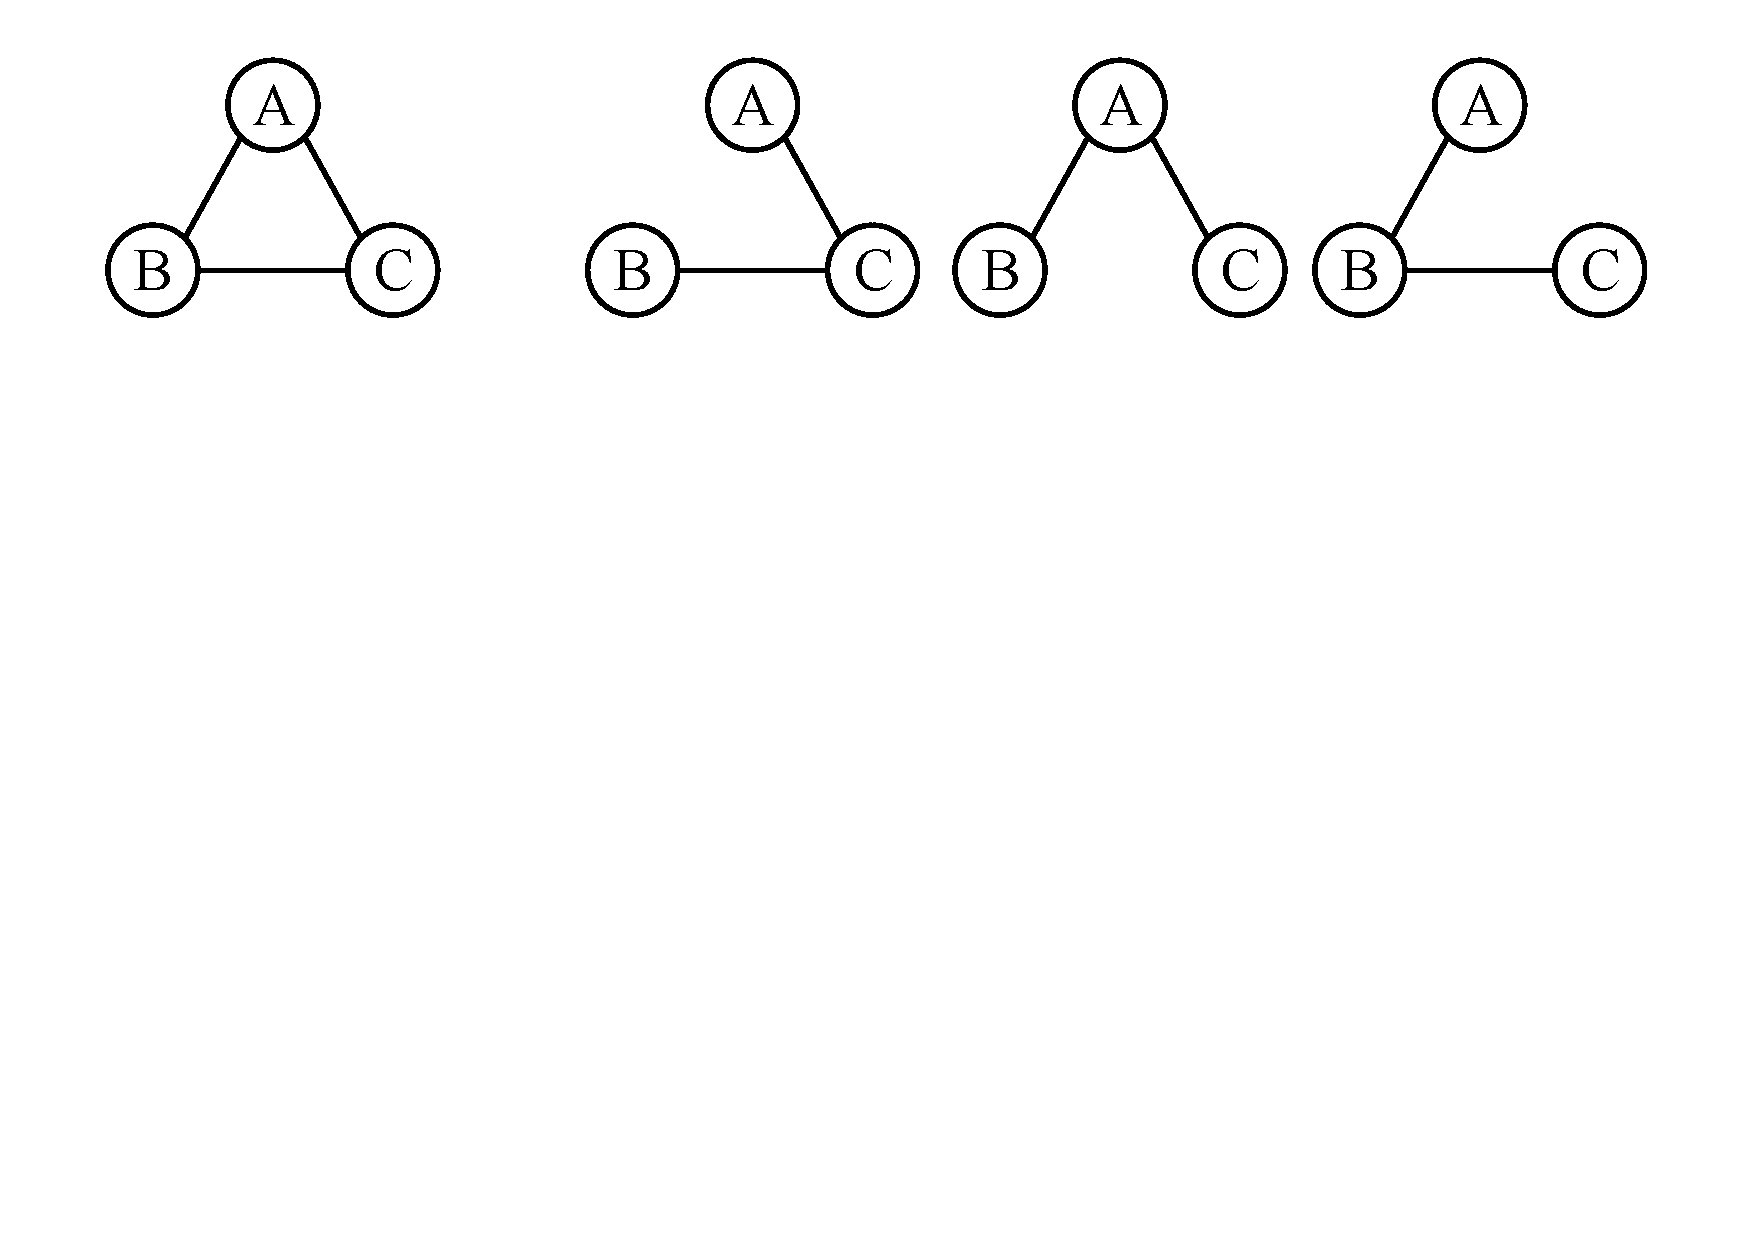
\includegraphics[scale=.4, clip,  trim=50 440 630 20]{img/arte/graphs-spanningTree.pdf}
    		
    		(a)
    	\end{minipage}
    	\begin{minipage}{0.65\textwidth}
    		\centering
    		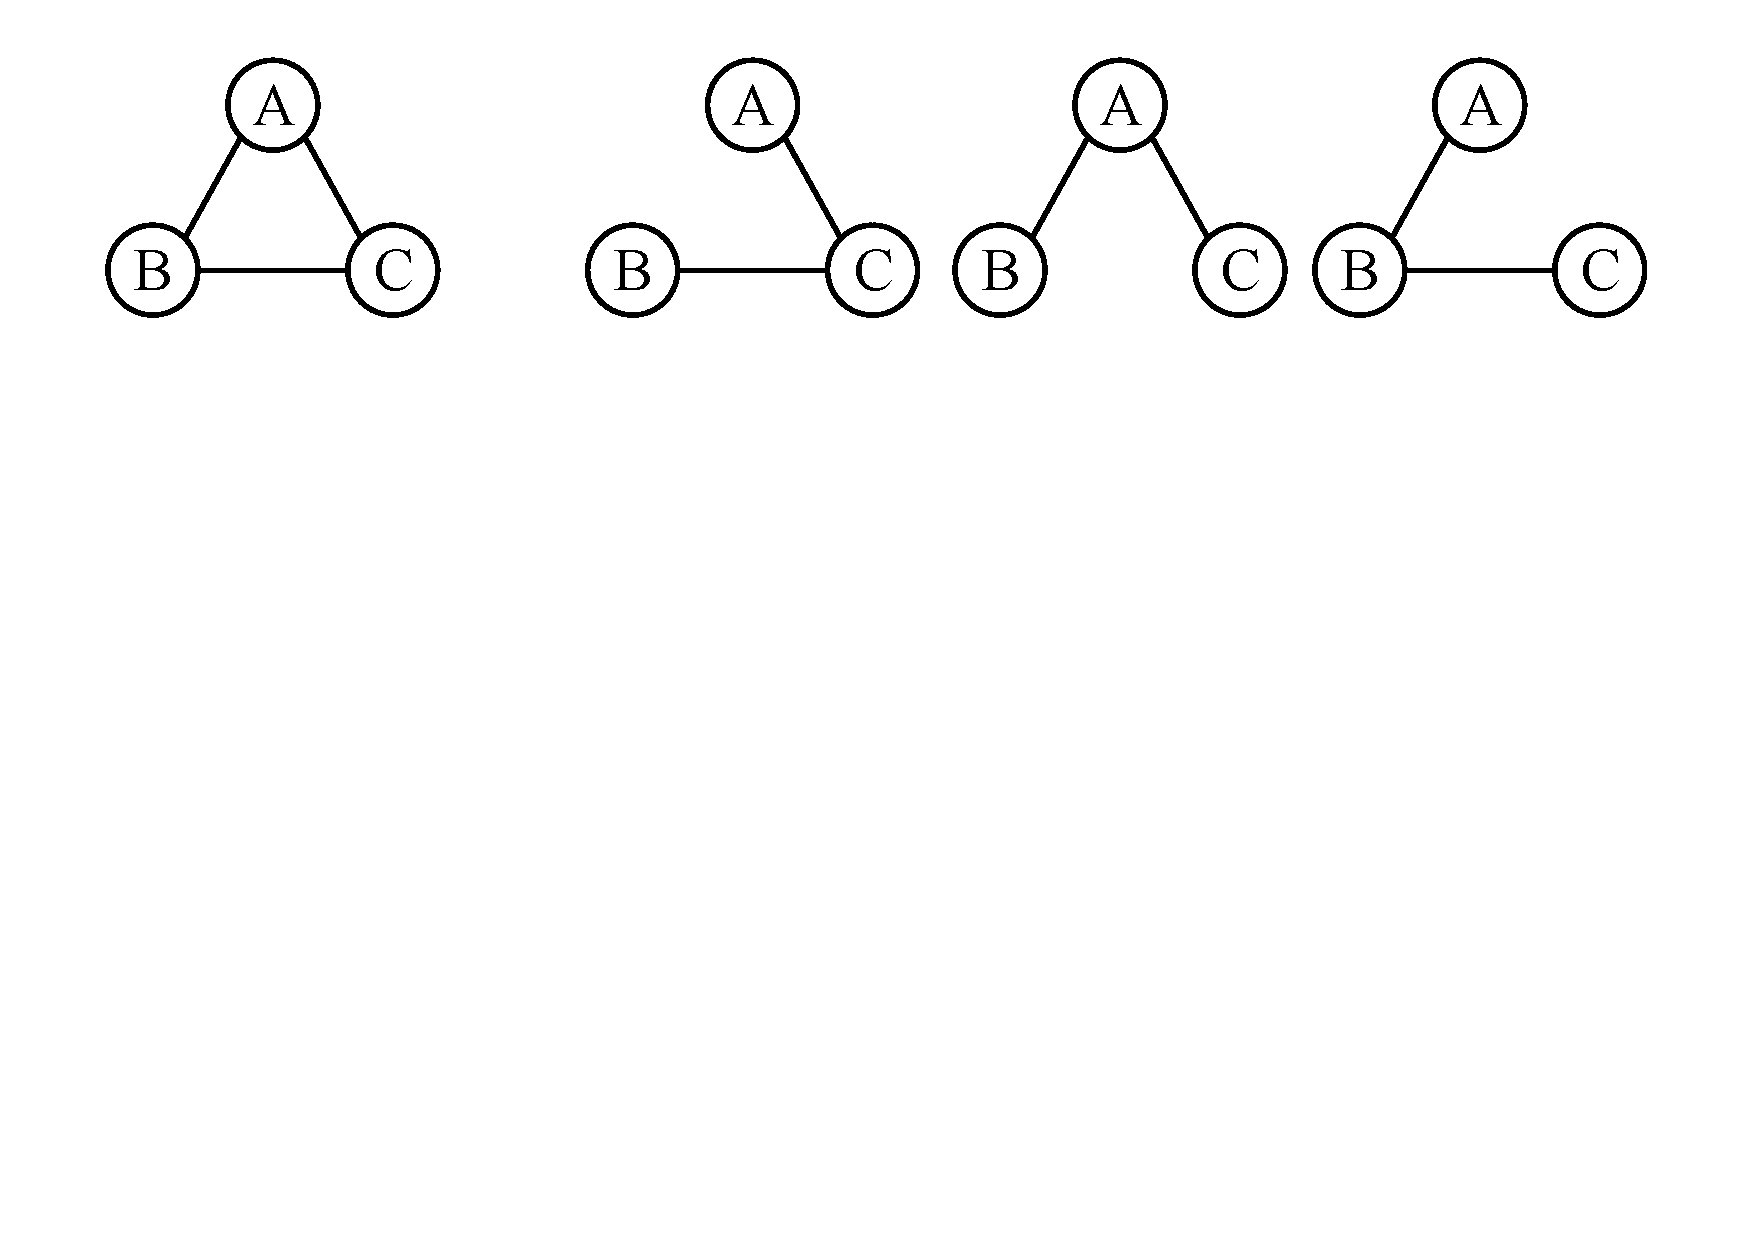
\includegraphics[scale=.4, clip, trim=280 440 50 20]{img/arte/graphs-spanningTree.pdf}
    		
    		(b)
    	\end{minipage}

    \caption{Ejemplos de árboles de expansión. (a) Grafo simple. (b)~Posibles árboles de expansión para el grafo.}
    \label{fig:spanningTree}
\end{figure}


\begin{figure}%[b]
    	\centering
    	\begin{minipage}{0.45\textwidth}
    		\centering
    		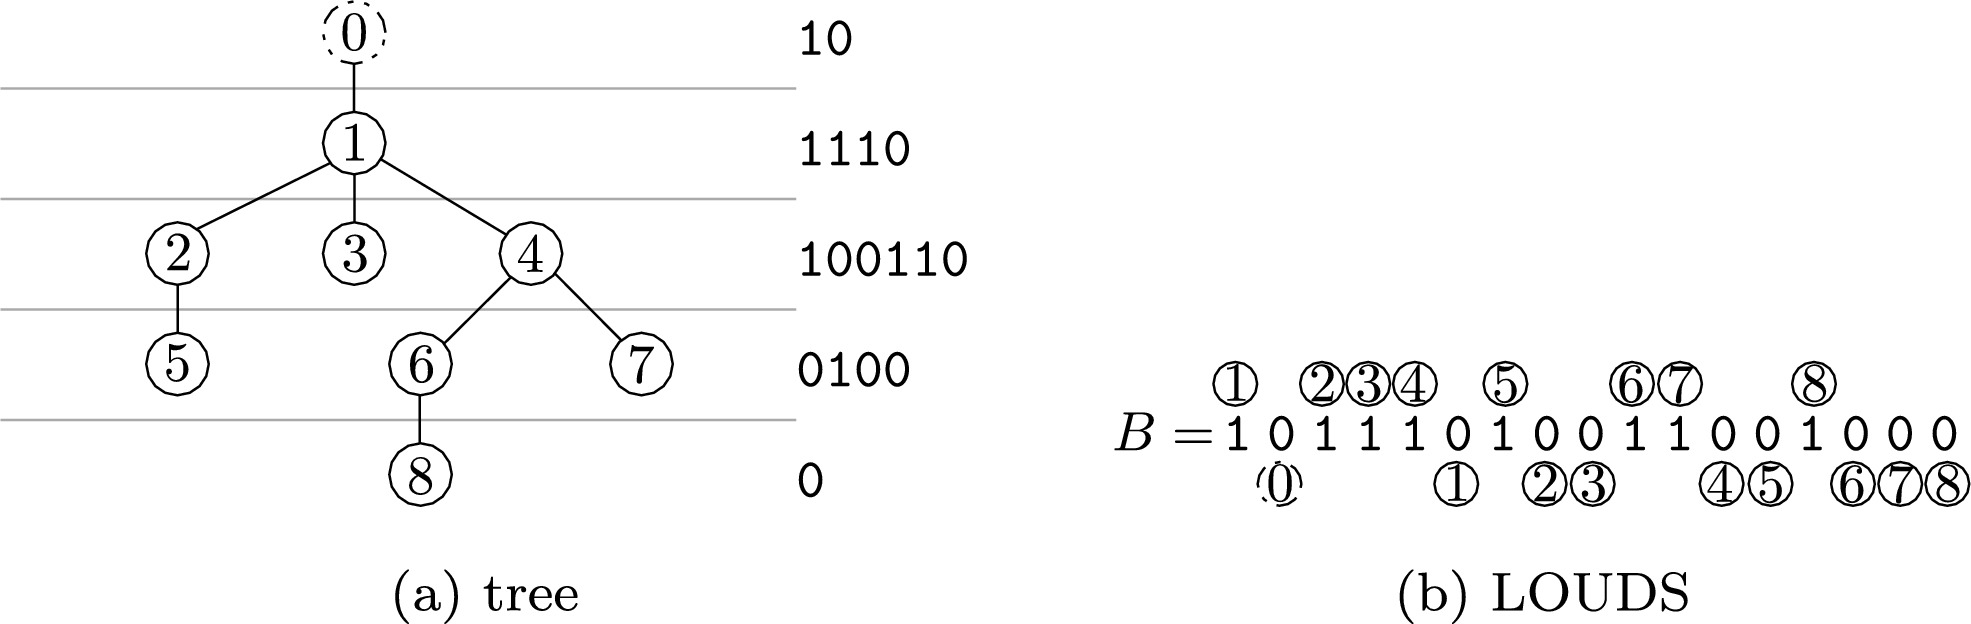
\includegraphics[scale=1.6, clip,  trim=10 16 140 0]{img/arte/LOUDS.jpg}
    		
    		(a)
    	\end{minipage}
    	\begin{minipage}{0.45\textwidth}
    		\centering
    		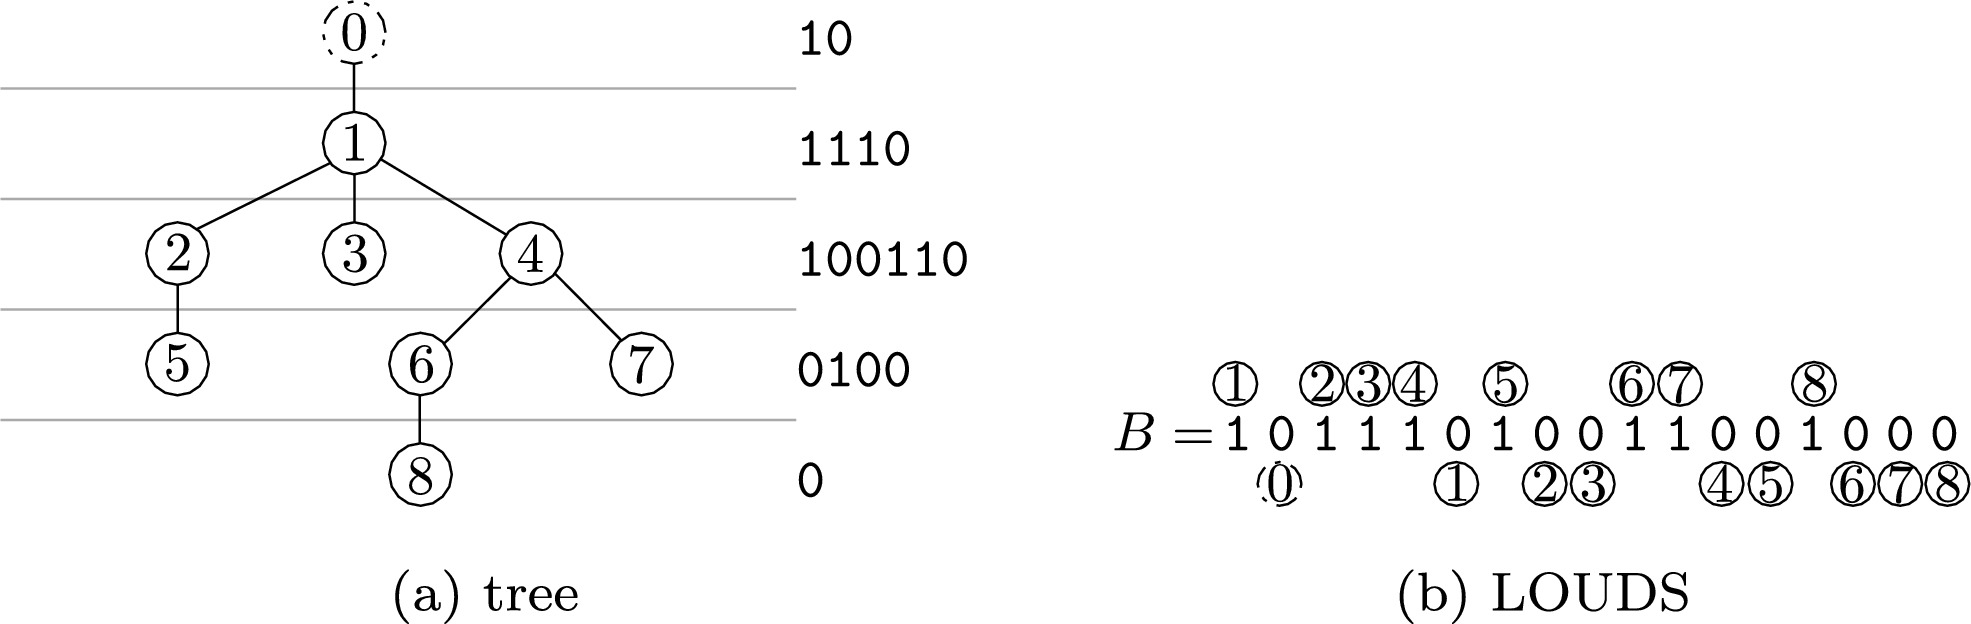
\includegraphics[scale=1.6, clip, trim=150 16 0 50]{img/arte/LOUDS.jpg}
    		
    		(b)
    	\end{minipage}

    \caption{Ejemplo de un árbol de expansión y su LOUDS. (a) Árbol de expansión y los bits generados por cada nivel de BFS. (b)~Bitmap $B$ de LOUDS.}
    \label{fig:LOUDS}
\end{figure}


Un árbol de expansión $T$ de un grafo $G$  con $n$ vértices y $m$ aristas, es un árbol que cubre todos los $n$ vértices de $G$ con la mínima cantidad de aristas posibles, sin generar ciclos. En la \autoref{fig:spanningTree} se muestran algunos ejemplos de árboles de expansión para un grafo simple. Un grafo con forma de árbol no tiene una cantidad de aristas adicionales muy alta, con respecto a un árbol de expansión.

La estructura \textit{LOUDS} \cite{jacobson1989space} está diseñada para comprimir árboles de expansión. Primero, por conveniencia, agrandan el árbol con un nodo \textit{super-raíz} artificial conectado al nodo raíz original. Luego van construyendo un bitmap $B$, avanzando por el árbol mediante BFS. Por cada nodo con $k$ hijos, se agregan $1^{k}0$ bits a $B$ (con $k=3$ sería $1110$). Esto representa a cada nodo del árbol dos veces: una vez con un $1$ cuando aparece el nodo como hijo, y con un $0$ cuando aparece como padre. Para $n$ nodos, el bitmap $B$ tiene $2n + 1$ bits de largo. En la \autoref{fig:LOUDS} se muestra un ejemplo de esta representación. Los nodos quedan identificados según el nivel de BFS donde aparecen.

Basado en esta idea, \textit{GLOUDS} \cite{fischer2016glouds} propone una nueva estructura para grafos con forma de árbol. Para esto define las siguientes características de un grafo $G$:

\begin{itemize}
	\item $c \leq n$, la cantidad de nodos raíz de $G$ (el tamaño mínimo del set de nodos desde donde se alcanzan todos los nodos restantes). 
	\item $k = m - n + 1$, la cantidad de aristas adicionales, con respecto al árbol de expansión $T$ de $G$.
	\item $h \leq k$, la cantidad de nodos adicionales.
\end{itemize}

Por simpleza, parten asumiendo que existe un nodo $r$ desde donde se pueden alcanzar todos los nodos restantes ($c = 1$). Desde $r$, realizan el recorrido por BFS de $G$, lo que llaman BFT, y $T_{G}^{BFT}$ el árbol resultante. Agrandan $T_{G}^{BFT}$ tal que por cada vértice $w$ ya visitado durante la BFT del nodo $v$ en una etapa anterior, realizan una copia llamada \textit{nodo sombra} y la agregan como hijo al nodo $v$ en $T_{G}^{BFT}$. Finalmente agregan el nodo \textit{super-raíz}, y llaman al árbol final $T_{G}$, que tiene exactamente $m + 2$ nodos. En la \autoref{fig:GLOUDS} se ilustra un ejemplo de GLOUDS, en (a) el grafo $G$, y en (b) el árbol $T_{G}$ final.

\input{figs/arte-glouds}

Luego proponen una representación de $T_{G}$ similar a la de LOUDS, pero que permita diferenciar los nodos sombra de los demás. Para esto, cambian el bitmap por una secuencia de trits, con posibles valores del conjunto $\{0, 1, 2\}$. Luego, la secuencia $B$ se genera de la misma manera, pero cuando aparece un nodo sombra en el recorrido BFS se agrega un $2$. Estos nodos no se vuelven a representar con un $0$. Le llaman al vector de trits $B$ CLOUDS, y tiene un largo de $n + m + c$ trits. En la \autoref{fig:LOUDS}~(c) se muestra el resultado para el ejemplo ya mencionado. Además, necesita un arreglo $H[0, k)$ que anota los nodos sombra que aparecen en B.


En este trabajo, se considerarán en la comparación final los métodos considerados más eficientes, en términos de construcción y resultados en compresión y tiempos de accesos a vecinos.



\section{Estructuras compactas} \label{sec:compactEstruct}
En esta sección se detallan las posibles estructuras compactas basadas en secuencias que se evaluarán para la compresión de la estructura planteada. Las operaciones básicas que permiten son \textbf{$Rank$}, \textbf{$Select$} y \textbf{$Access$}, las cuales se detallan a continuación:

\begin{itemize}
	\item \textbf{$Rank_{S}(a, i)$}: Cuenta las ocurrencias del símbolo $a$ hasta la posición $i$ en la secuencia $S$.
	\item \textbf{$Select_{S}(a, i)$}: Encuentra la posición de la ocurrencia $i$ del símbolo $a$ en la secuencia $S$.
	\item \textbf{$Access_{S}(i)$}: Retorna el símbolo en la posición $i$ de la secuencia $S$.
\end{itemize}

\textcolor{red}{No tengo claridad de cómo presentar los siguientes trabajos, sobre todo las secuencias binarias, sin tener que entras más en detalle de la teoría.}

\subsection{Secuencias binarias}
Existen varias propuestas de estructuras compactas para secuencias binarias, siendo una de las más usadas la de Raman, Raman, Rao \cite{raman2002succinct}, que logran las funciones de \textit{Rank} y \textit{Select} en tiempo constante. Además, con $B[1, n]$ un bitmap de largo $n$ con $n_{0}$ ceros y $n_{1}$ unos, en espacio requiere $nH_{0}(B) + o(n)$ bits, siendo $H_{0}(B)$ la entropía de orden cero de $B$: 

\begin{equation}
	H_{0}(B) = \frac{n_{0}}{n} \log\frac{n}{n_{0}} + \frac{n_{1}}{n} \log\frac{n}{n_{1}}
\end{equation}

Okanohara y Sadakane \cite{DBLP:journals/corr/abs-cs-0610001} proponen una mejora que elimina el costo de $o(n)$ en bits para bitmaps poco densos, y si bien el costo para la operación \textit{Select} se mantiene, aumenta para \textit{Rank}.


\subsection{Wavelet Tree y Wavelet Matrix}
Grossi, Gupta y Vitter \cite{grossi2003high} proponen una estructura llamada \textbf{wavelet tree} para codificar secuencias, la cual consiste en un árbol binario donde la raíz y cada nodo interno son bitmaps. Si el símbolo en la secuencia pertenece a la primera mitad del alfabeto de la secuencia de entrada, se marca con un $0$ en su correspondiente bit del bitmap asociado, y se escribe en el nodo hijo izquierdo. Si pertenece a la segunda mitad del alfabeto, se marca con un $1$ en el bitmap y se escribe en el nodo hijo derecho. En la \autoref{fig:wavelet-tree} se muestran dos ejemplos de wavelet-tree. En (a) se tiene un ejemplo simple de la subdivisión de una secuencia ordenada. En (b) se presenta un ejemplo práctico de los alfabetos, la subdivisión de la secuencia y los bitmaps por nodo del wavelet-tree.

\begin{figure}%[b]
    	\centering
    	\begin{minipage}{0.4\textwidth}
    		\centering
    		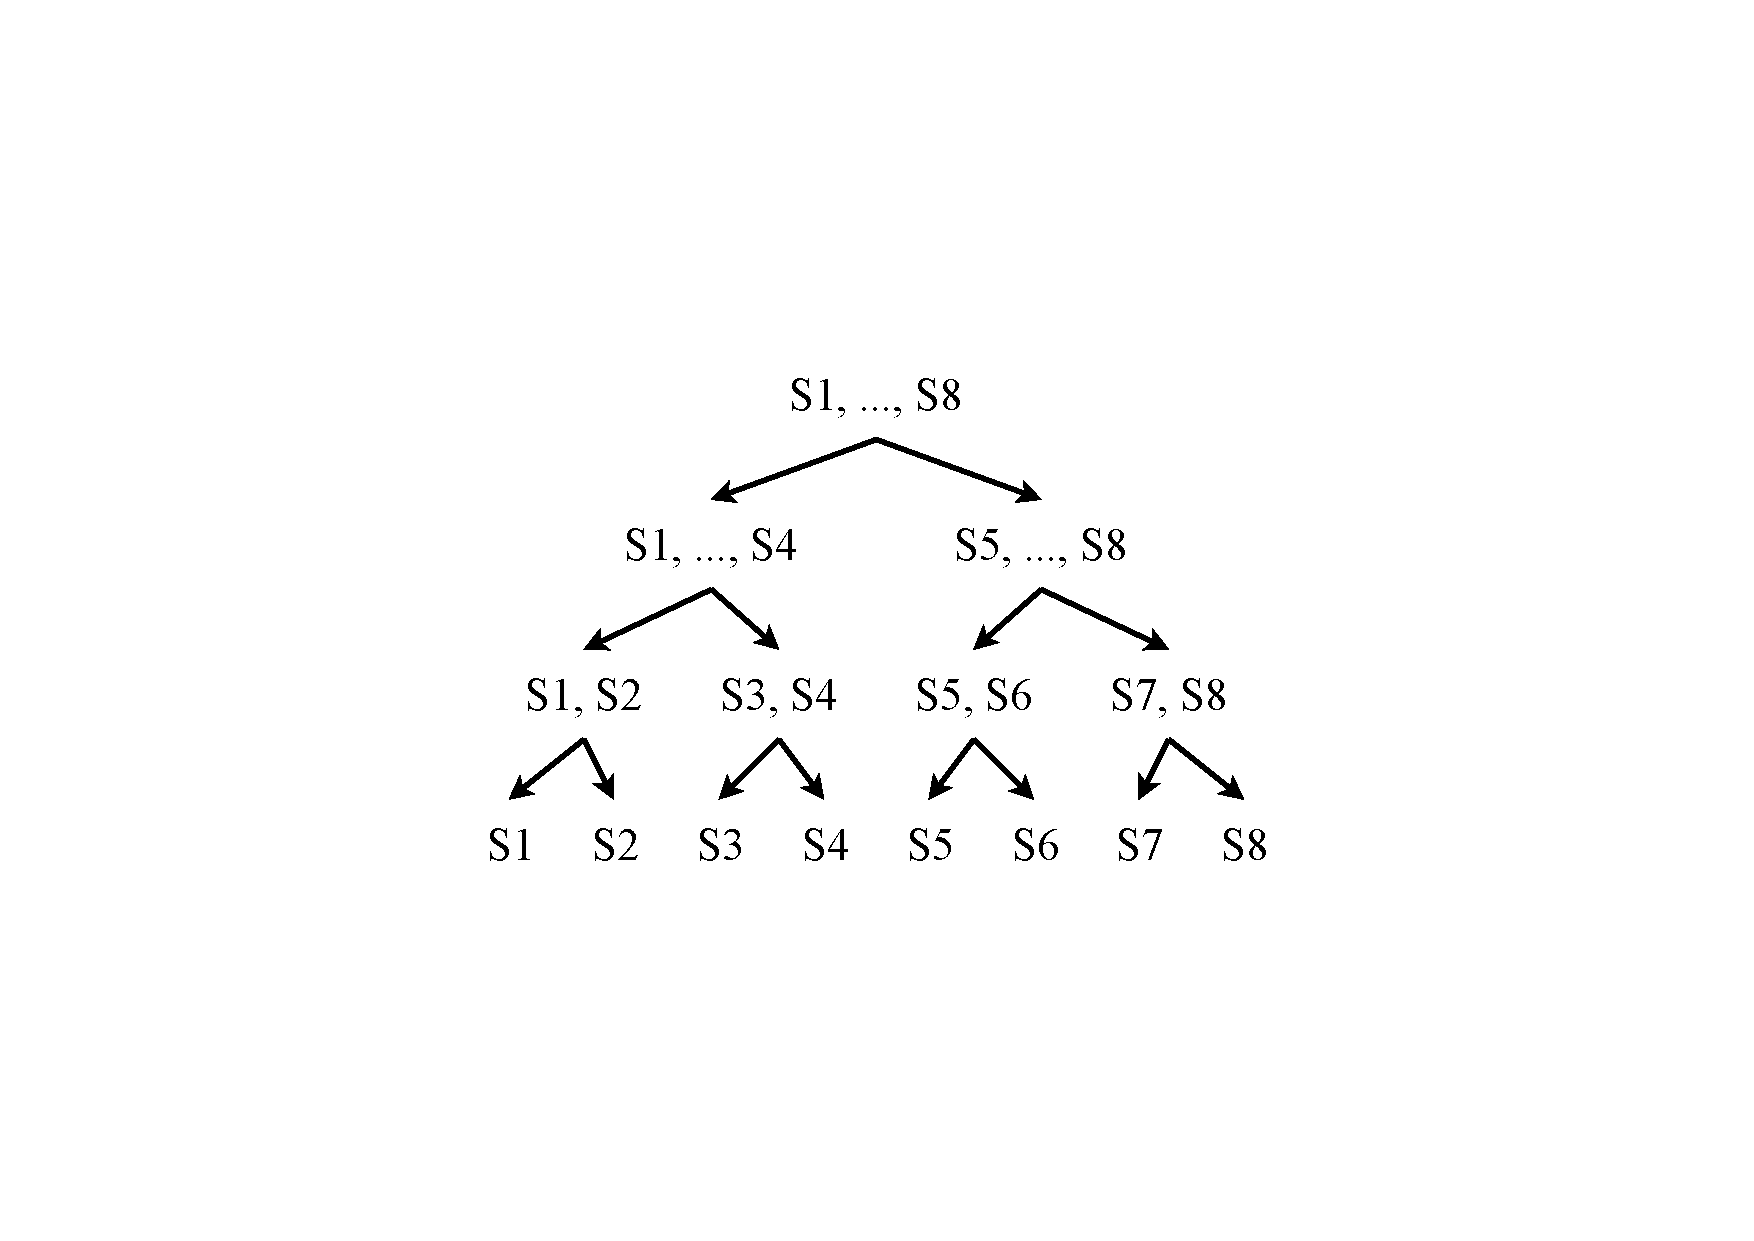
\includegraphics[scale=.45, clip,  trim=230 182 230 180]{img/arte/graphs-wavelet-tree.pdf}
    		
    		(a)
    	\end{minipage}
    	\begin{minipage}{0.5\textwidth}
    		\centering
    		%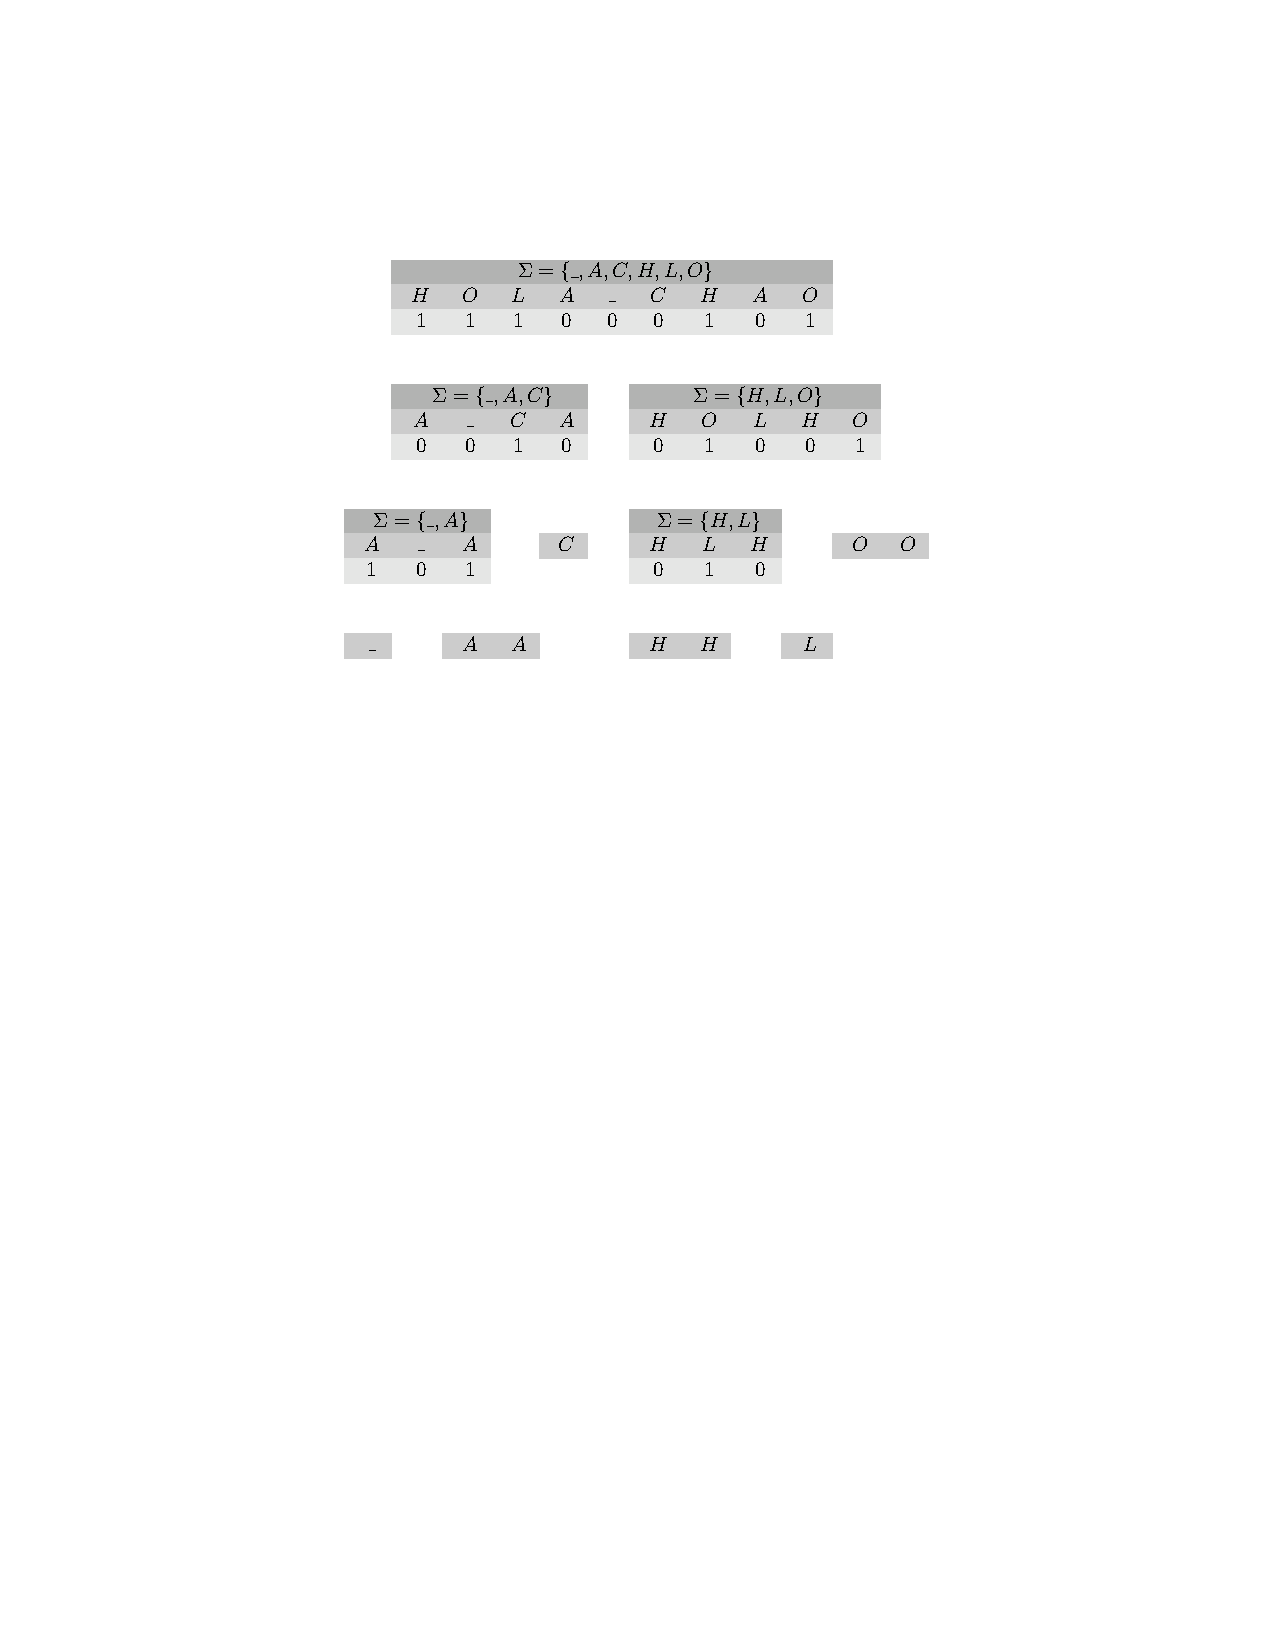
\includegraphics[scale=.8, clip, trim=150 475 150 120]{img/arte/wavelet-tree2.pdf}
    		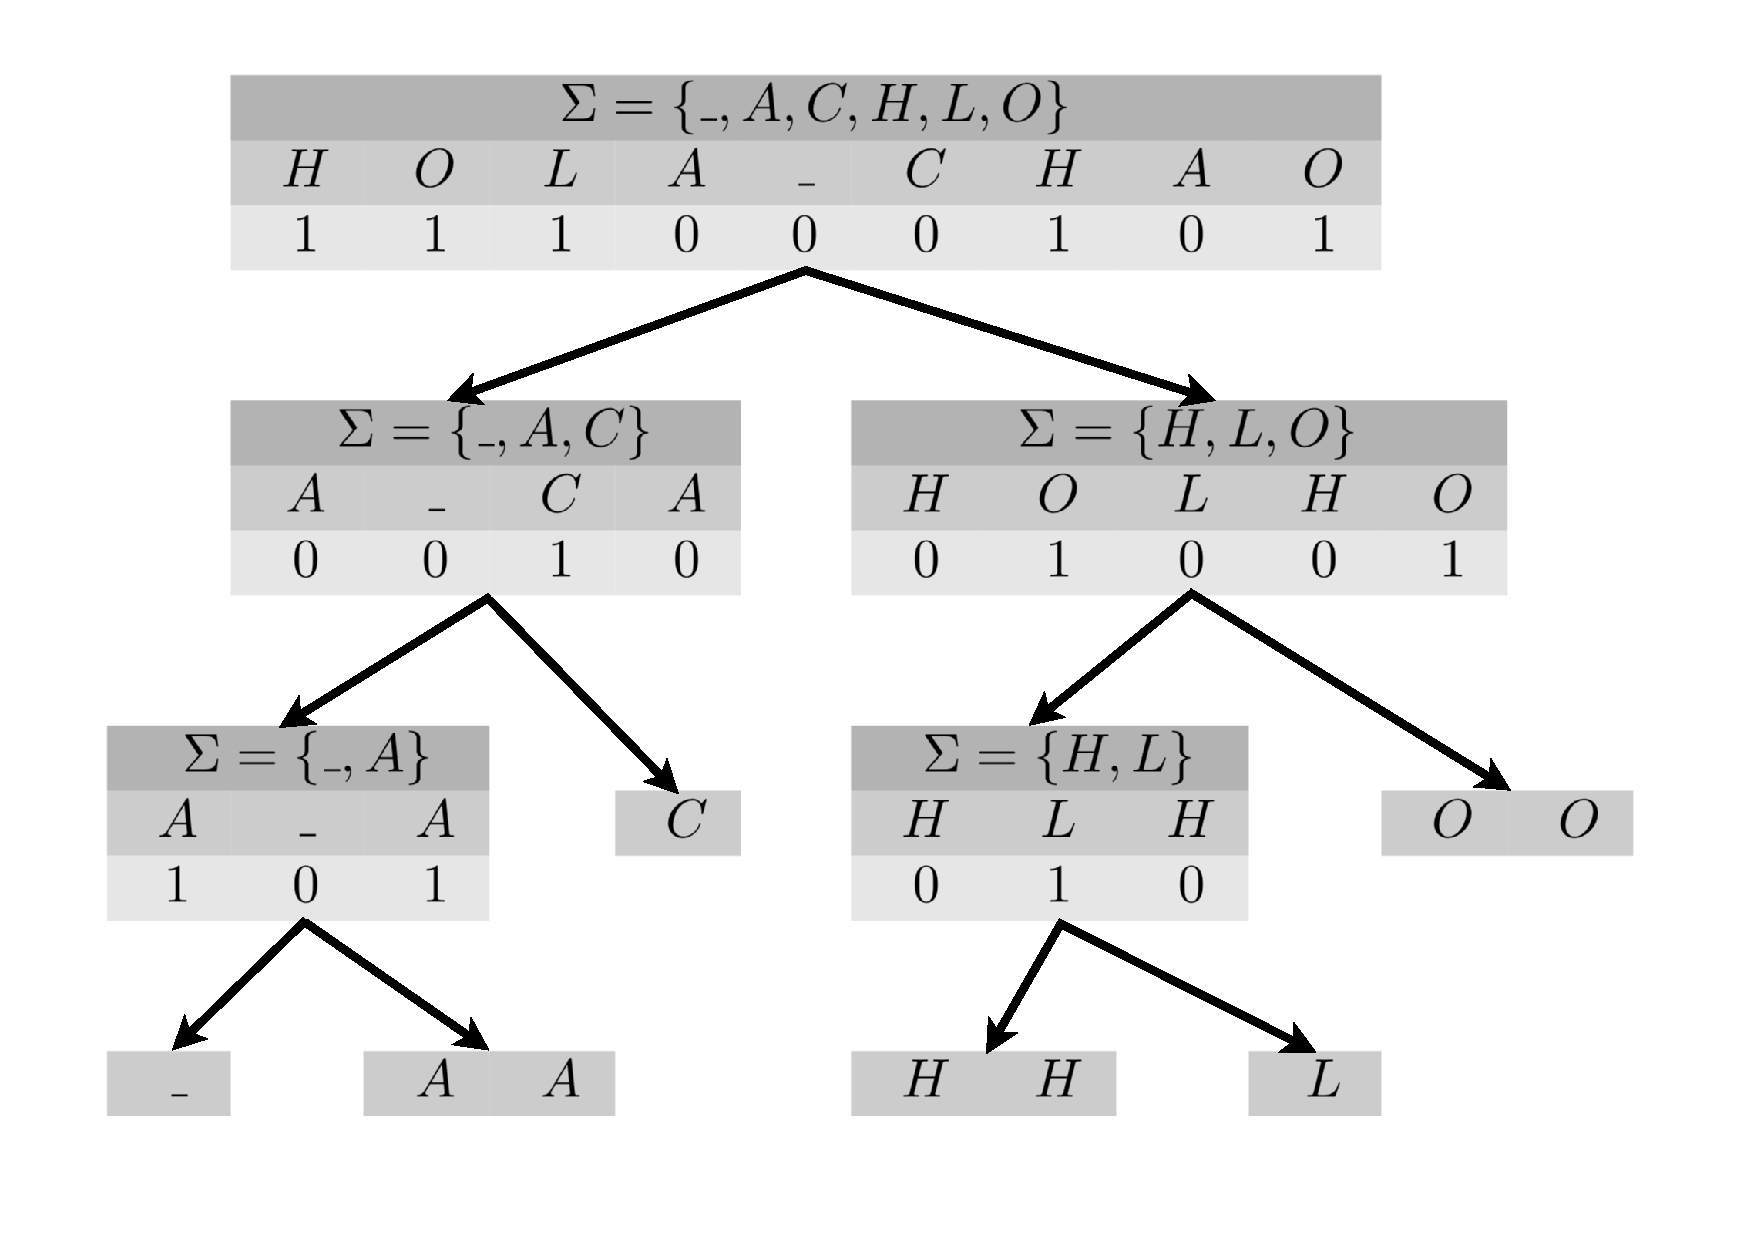
\includegraphics[scale=.3, clip, trim=0 0 0 0]{img/arte/graphs-wavelet-tree2.pdf}

    		(b)
    	\end{minipage}

    \caption{Ejemplos de wavelet-tree. (a) Ejemplo básico de subdivisión de secuencia ordenada. (b) Ejemplo práctico con alfabetos y bitmaps por nodo.}
    \label{fig:wavelet-tree}
\end{figure}

%    		\begin{tabular}{cccccccccccccc}
%	& & \multicolumn{9}{c}{\cellcolor{G} $\Sigma = \{\_,A, C, H, L, O\}$} & & & \\
%	& & \cellcolor{LG} $H$ & \cellcolor{LG} $O$ & \cellcolor{LG} $L$ & \cellcolor{LG} $A$ & \cellcolor{LG} $\_$ & \cellcolor{LG} $C$ & \cellcolor{LG} $H$ & \cellcolor{LG} $A$ & \cellcolor{LG} $O$ & & & \\
%	& & \cellcolor{LLG} $1$ & \cellcolor{LLG} $1$ & \cellcolor{LLG} $1$ & \cellcolor{LLG} $0$ & \cellcolor{LLG} $0$ & \cellcolor{LLG} $0$ & \cellcolor{LLG} $1$ & \cellcolor{LLG} $0$ & \cellcolor{LLG} $1$ & & & \\
%	\\
%	\\
%	 & & \multicolumn{4}{c}{\cellcolor{G} $\Sigma = \{\_,A, C\}$} & & \multicolumn{5}{c}{\cellcolor{G} $\Sigma = \{H, L, O\}$} & & \\
%	& & \cellcolor{LG} $A$ & \cellcolor{LG} $\_$ & \cellcolor{LG} $C$ & \cellcolor{LG} $A$ &  & \cellcolor{LG} $H$ & \cellcolor{LG} $O$ & \cellcolor{LG} $L$ & \cellcolor{LG} $H$ & \cellcolor{LG} $O$ &  & \\
%	& & \cellcolor{LLG} 0 & \cellcolor{LLG} 0 & \cellcolor{LLG} 1 & \cellcolor{LLG} 0 &  & \cellcolor{LLG} 0 & \cellcolor{LLG} 1 & \cellcolor{LLG} 0 & \cellcolor{LLG} 0 & \cellcolor{LLG} 1 &  & \\
%	\\
%	\\
%	& \multicolumn{3}{c}{\cellcolor{G} $\Sigma = \{\_,A\}$} & & & &  \multicolumn{3}{c}{\cellcolor{G} $\Sigma = \{H, L\}$} & & & & \\
%	& \cellcolor{LG} $A$ & \cellcolor{LG} $\_$ & \cellcolor{LG} $A$ &  & \cellcolor{LG} $C$	 &  & \cellcolor{LG} $H$ & \cellcolor{LG} $L$ & \cellcolor{LG} $H$ &  & \cellcolor{LG} $O$ & \cellcolor{LG} $O$ & \\
%	& \cellcolor{LLG} 1 & \cellcolor{LLG} 0 & \cellcolor{LLG} 1 &  &  &  & \cellcolor{LLG} 0 & \cellcolor{LLG} 1 & \cellcolor{LLG} 0 &  &  &  &  \\
%	\\
%	\\
%	& \cellcolor{LG} $\_$ & & \cellcolor{LG} $A$ & \cellcolor{LG} $A$ & & & \cellcolor{LG} $H$ & \cellcolor{LG} $H$ & & \cellcolor{LG} $L$ & & & \\ 
%\end{tabular}

Se construye de la siguiente manera. Dada una secuencia $S$ de largo $n = |S|$, donde $S[i] \in \Sigma$ y $\sigma = |\Sigma|$, se tiene: La raíz del árbol consiste en un bitmap $B$ donde $B[i] = 0$ si $S[i] \in [0, \frac{\sigma}{2}]$ y $B[i] = 1$ si $S[i] \in [\frac{\sigma}{2} + 1, \sigma]$. El siguiente nivel del árbol se construye basado en los símbolos asociados al nodo por el bitmap $B$ padre. Para $B[i] = 0$, se crea el bitmap hijo de la izquierda, y el alfabeto asociado a esos símbolos nuevamente se divide en dos, asignando valor a dicho bitmap siguiendo el mismo procedimiento descrito anteriormente. De manera similar, para $B[i] = 1$ se crea el bitmap derecho y se sigue el mismo procedimiento. Esto se repite por cada nodo hasta llegar a símbolos únicos en cada nodo terminal. Se requiere guardar los punteros a cada nodo hijo izquierdo y derecho, con los que se permite la navegación por el árbol.

Mejorando la propuesta de wavelet tree \cite{grossi2003high}, Claude, Navarro y Ordóñez \cite{claude2015wavelet} proponen una nueva estructura llamada \textbf{wavelet matrix}. Primero crean una versión de wavelet tree sin punteros, reemplazando cada bitmap por nodo por solo un bitmap por nivel, y contando la cantidad de ceros pueden determinar las subdivisiones pertinentes en cada nivel. 

Luego, para crear la wavelet matrix, liberan a la estructura de la suposición que los hijos de un nodo $v$ deben ir alineados. Esto les permite diseñar un mecanismo de clasificación mas sencillo entre un nivel y otro: todos los ceros pasan a la izquierda y todos los unos a la derecha. Por cada nivel, guardan en un entero $z_{\ell}$ la cantidad de ceros del nivel $\ell$. En la \autoref{fig:wavelet-matrix} se presentan en (a) un wavelet tree de ejemplo, en (b) su correspondiente wavelet tree sin punteros, y en (c) su wavelet matrix, donde las líneas verticales representan el valor de $z_{\ell}$ para cada nivel.

\begin{figure}%[b]
    	\centering
    	\begin{minipage}{0.3\textwidth}
    		\centering
    		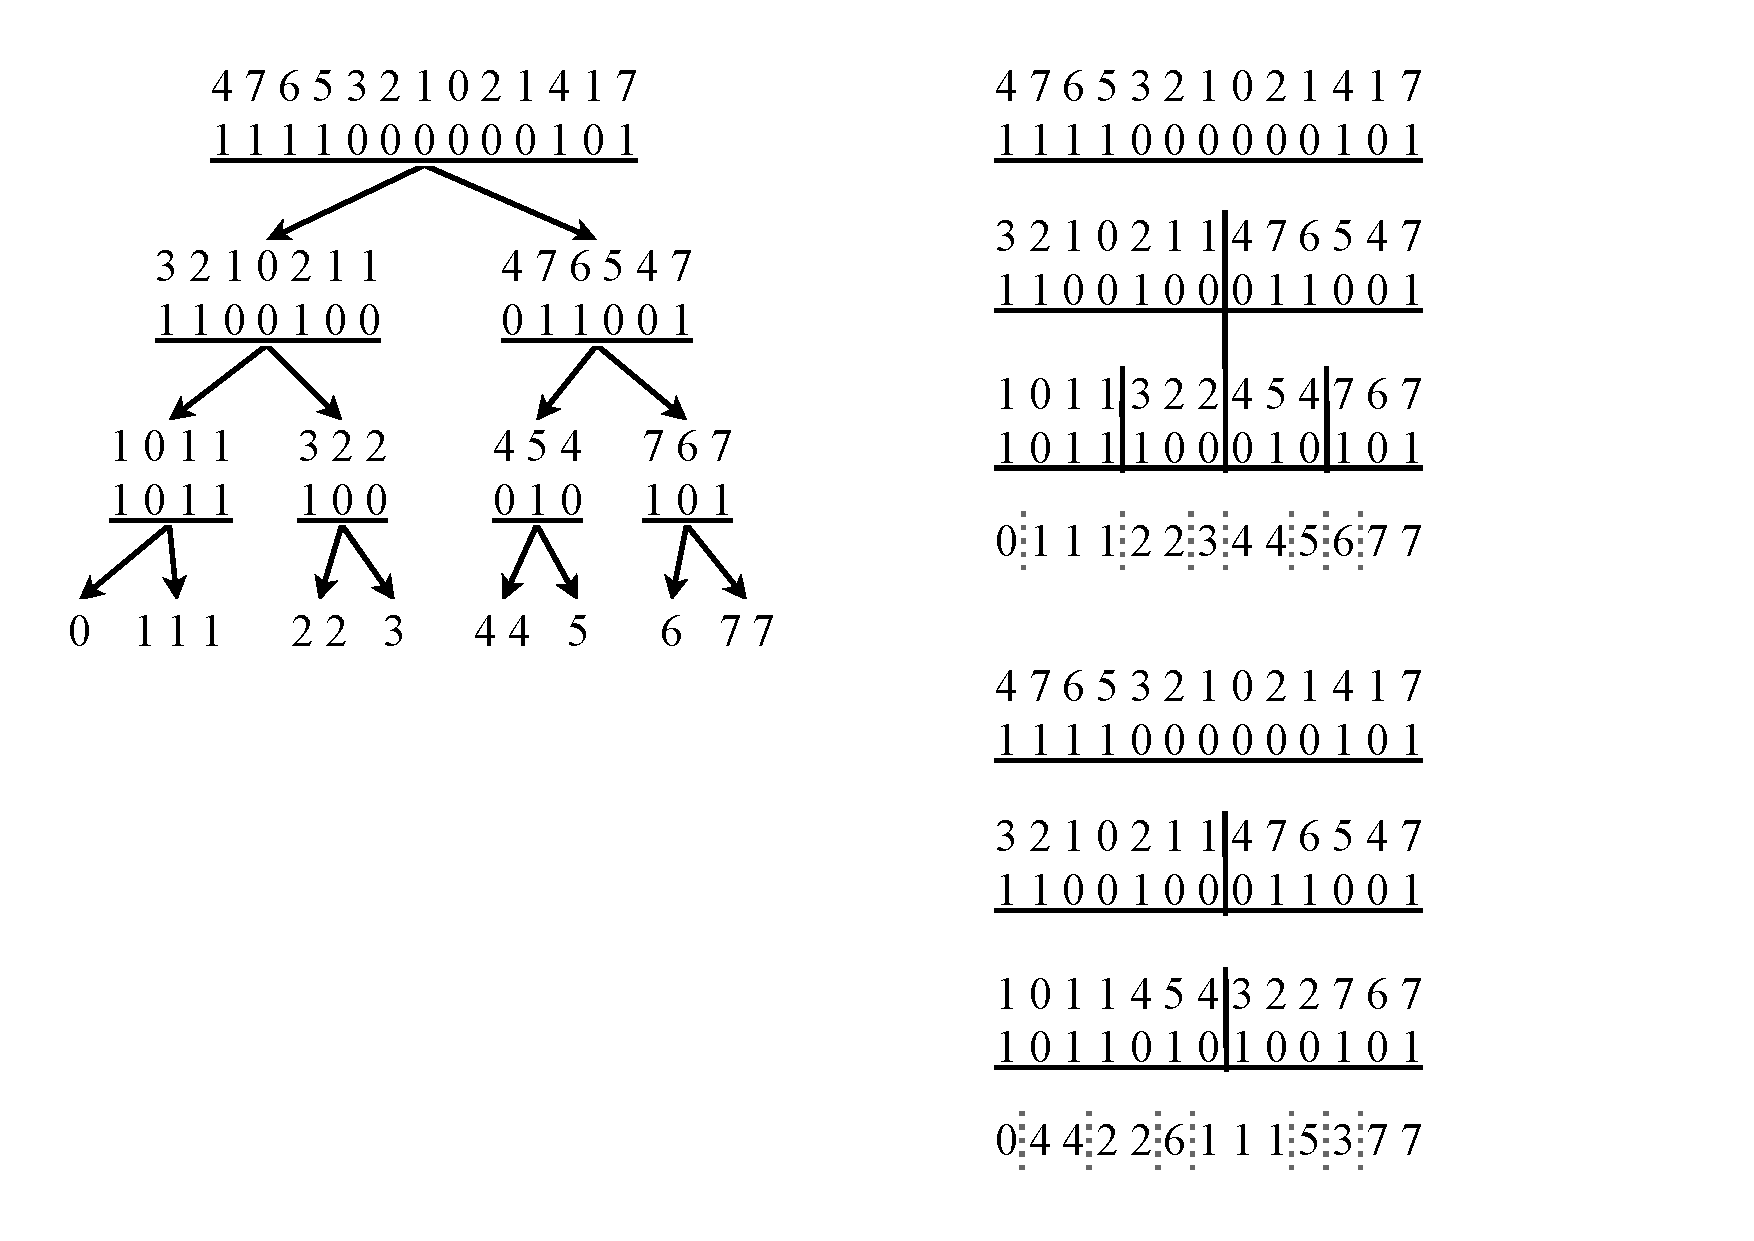
\includegraphics[scale=.4, clip,  trim=30 280 440 30]{img/arte/graphs-wavelet-matrix.pdf}
    		
    		(a)
    	\end{minipage}
    	\begin{minipage}{0.3\textwidth}
    		\centering
    		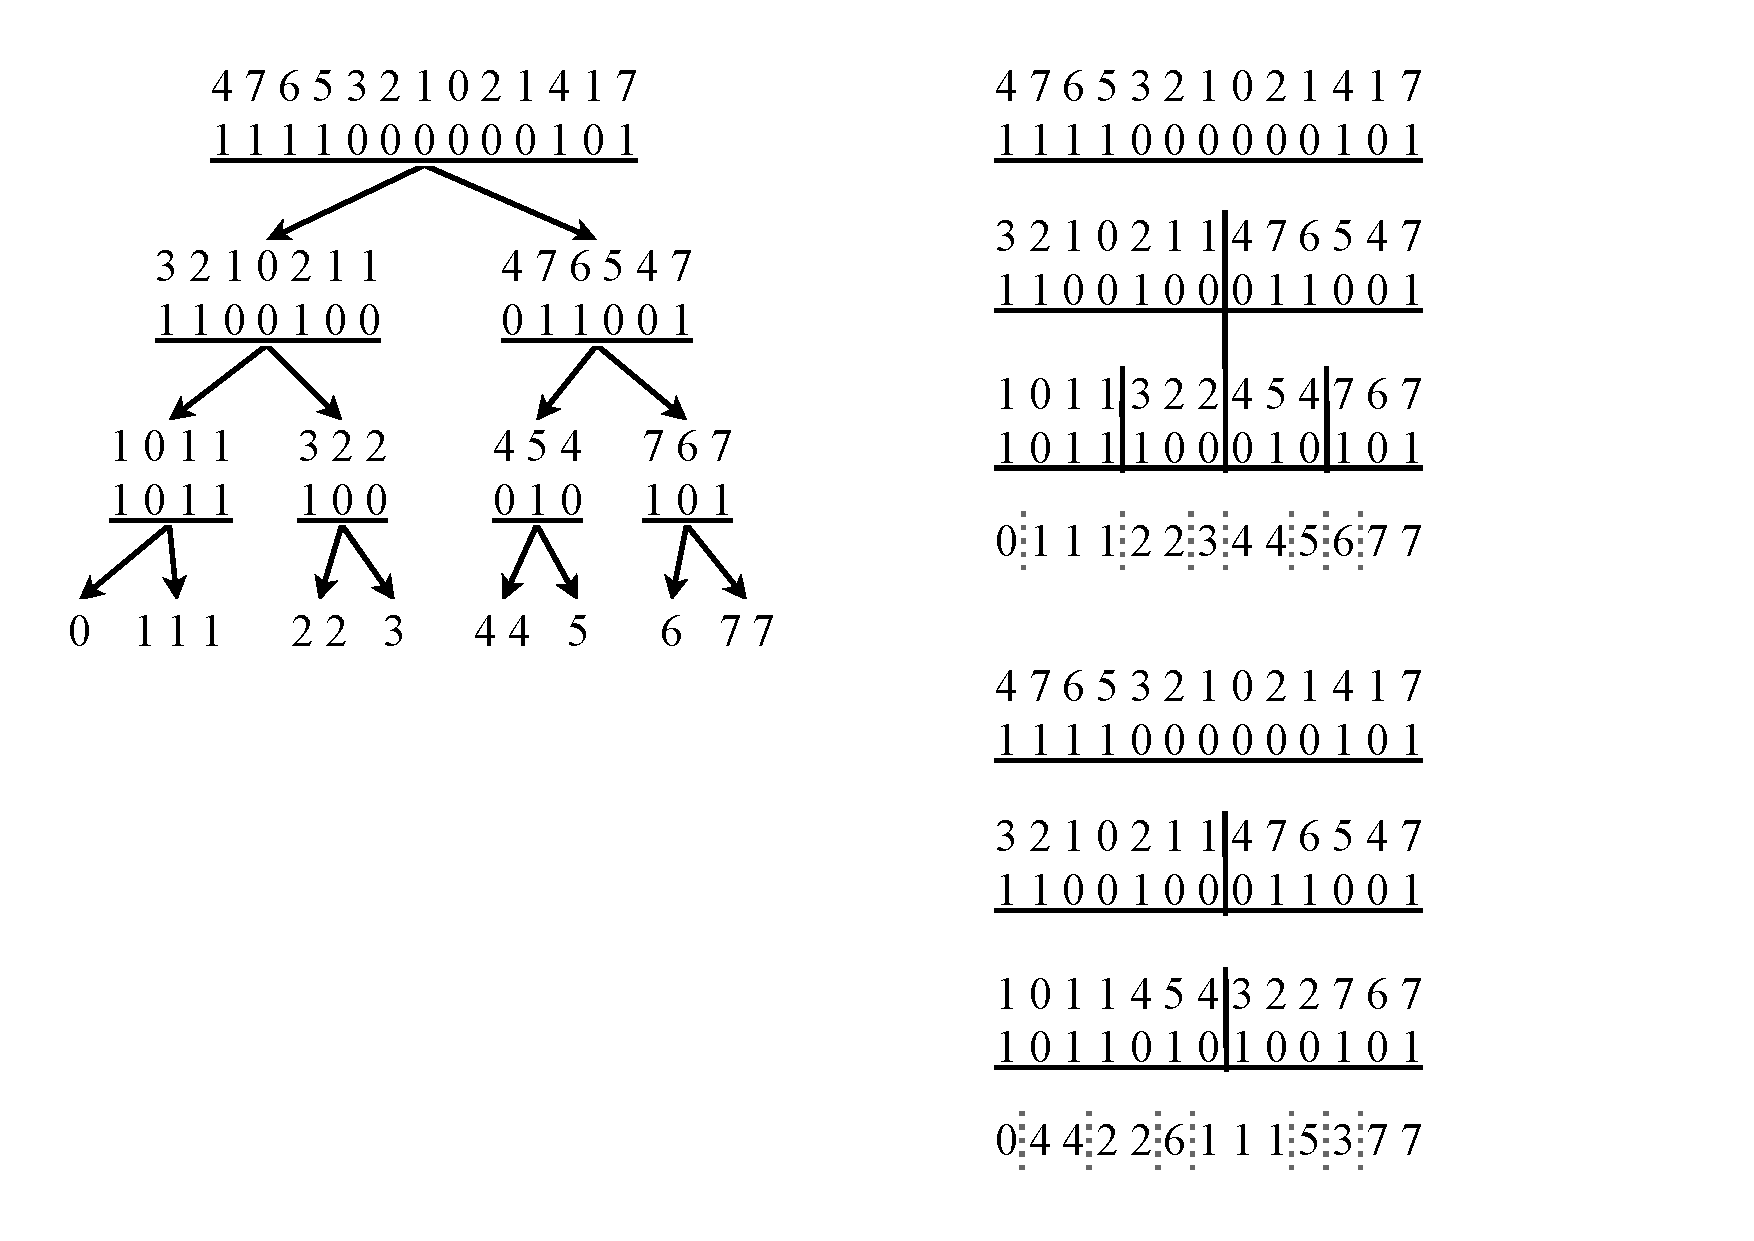
\includegraphics[scale=.45, clip, trim=470 320 170 30]{img/arte/graphs-wavelet-matrix.pdf}

    		(b)
    	\end{minipage}
    	\begin{minipage}{0.3\textwidth}
    		\centering
    		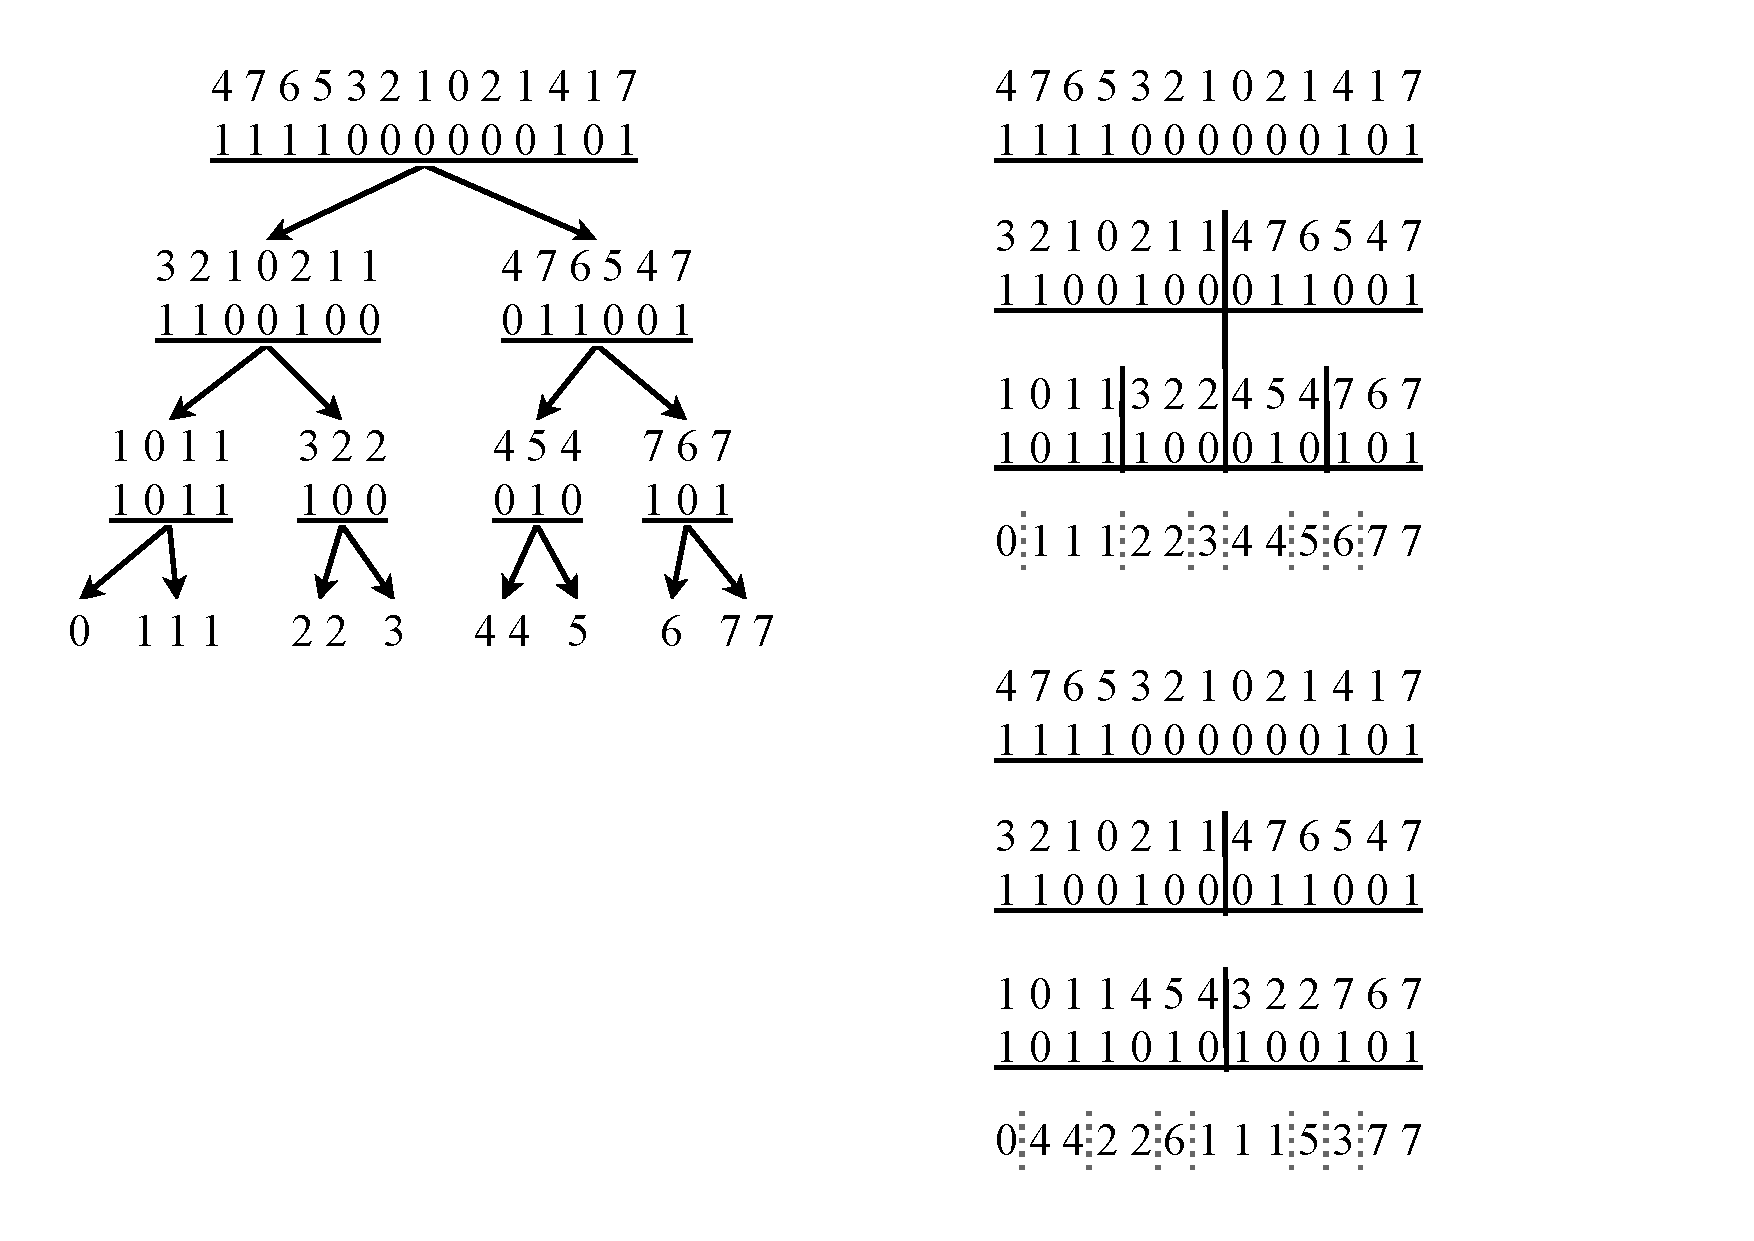
\includegraphics[scale=.45, clip, trim=470 33 170 317]{img/arte/graphs-wavelet-matrix.pdf}

    		(c)
    	\end{minipage}

    \caption{Ejemplos para wavelet-matrix. (a) Un wavelet tree. (b) El mismo wavelet tree sin punteros. (c) La wavelet matrix correpondiente.}
    \label{fig:wavelet-matrix}
\end{figure}


También prueban otras alternativas de representación, como usar Huffman \cite{huffman1952method} tanto para la representación sin punteros del wavelet-tree como para la wavelet matrix. Su resultado apunta a la superioridad tanto en tiempo como espacio en disco de wavelet matrix sobre wavelet-tree, lo que se tendrá en consideración a la hora de evaluarlos como alternativas de compresión.

\subsection{SDSL - Succinct Data Structure Library}
Gog, Beller, Moffat y Petri \cite{gbmp2014sea} desarrollan la librería \texttt{SDSL}\footnote{\url{https://github.com/simongog/sdsl-lite}} (Succinct Data Structure Library), desarrollada en \texttt{C++11} y registrada bajo \texttt{GPLv3}, donde se pueden utilizar las estructuras planteadas en las secciones anteriores, entre muchas otras más.



\section{Detección de cliques maximales} \label{sec:Cliques}
La detección de cliques maximales en un grafo es un problema NP-Hard \cite{karp1972reducibility}. Se han buscado una solución desde varios enfoques \cite{bron1973algorithm, eblen2012maximum, hendrix2010theoretical, bomze1999maximum, eppstein2010listing, eppstein2011listing}. siendo la más destacada para este trabajo lo propuesto por Eppstein y Strash \cite{eppstein2011listing}, basado en el trabajo de Eppstein, Löffler y Strash \cite{eppstein2010listing}, enfocado a grafos poco densos.

Eppstein et al. \cite{eppstein2010listing} presentan una modificación al algoritmo de Bron–Kerbosch \cite{bron1973algorithm}, que permite encontrar los cliques maximales de un grafo poco denso, con $n$ nodos y \textit{degeneracy} $d$, en un tiempo $O(dn3^{d/3})$.

Antes de detallar el funcionamiento de los algoritmos, primero es necesario definir lo siguiente: Sea un grafo $G = (V, E)$, con $n$ vértices y $m$ aristas. Para un vértice $v$ se define $\Gamma(v)$ como el set $\{w | (v, w) \in E\}$, llamado la \textit{vecindad} de $v$, y similarmente para un subset $W \subset V$ se define $\Gamma(W)$ como el set $\cap_{w \in W} \Gamma(w)$, llamado la \textit{vecindad común} de todos los vértices en $W$.

El algoritmo de Bron–Kerbosch \cite{bron1973algorithm} es un algoritmo \textit{backtracking} recursivo, sencillo y muy usado para encontrar el listado de cliques maximales de un grafo. Una llamada recursiva entrega tres sets separados de nodos: $R$, $P$, y $X$. $R$ es un clique (posiblemente no maximal), y $P \cup X = \Gamma(R)$ son todos los vértices adyacentes a cada vértice en $R$. Los nodos en $P$ son aquellos que serán considerados para añadirse a $R$, y los pertenecientes a $X$ deben ser excluidos del clique. El algoritmo elige un candidato en $v \in P$ para añadirlo al clique $R$, realiza una llamada recursiva con $v$ ya movido de $P$ a $R$, y con $X$ restringido a los vecinos de $v$. Cuando la llamada recursiva retorna, $v$ se mueve a $X$ para evitar trabajo redundante. Cuando la recursión llega al punto donde $P$ y $X$ están vacíos, $R$ es reportado como un clique maximal. Para obtener todos los cliques maximales, se debe iniciar la recursión con $P$ igual a todos los nodos del grafo, y $R$ con $X$ vacíos.

También describen la heurística llamada \textit{pivoting}, que limita la cantidad de llamadas recursivas realizadas por el algoritmo. Para cualquier nodo $u \in P \cup X$, llamado \textit{pivot}, cualquier clique maximal debe contener algún nodo no vecino de $u$, incluido si mismo. Por tanto, se retrasa que los vértices en $P \cap \Gamma(u)$ sean añadidos al clique, beneficiando realizar menos llamadas recursivas. Tomita et al. \cite{tomita2006worst} demuestran que eligiendo el \textit{pivot} $u$ para maximizar $|P \cap \Gamma(u)|$, se garantiza un orden de tiempo $O(3^{n/3})$.

Eppstein et al. \cite{eppstein2010listing} prueban que el orden de procesamiento de los vértices de $G$ por el algoritmo de Bron–Kerbosch también es importante. Lo primero que hacen es un ordenamiento por \textit{degeneracy} de los nodos del grafo, y en ese orden hacen las llamadas recursivas del algoritmo, usando la regla de \textit{pivot} de Tomita. En la \autoref{fig:degenOrder} se ilustra un ejemplo de ordenamiento por \textit{degeneracy}. Gracias a esto, garantizan que su algoritmo propuesto logra listar todos los cliques maximales en un tiempo $O(dn3^{d/3})$.

arte-degenOrder




%%%%%%%%%%%%%%%%%%%%%%%%%%%%%%%%%%%%%%%%%%%%%%%%%%%%%%%%%%%%%%%%%%%%%%%%%%%%%%%%
%
% Paso 16: Cuerpo de la Tesis
% 
%%%%%%%%%%%%%%%%%%%%%%%%%%%%%%%%%%%%%%%%%%%%%%%%%%%%%%%%%%%%%%%%%%%%%%%%%%%%%%%%


\chapter{MÉTODO DE COMPRESIÓN PROPUESTO}\label{chap:clustering}
\vskip 3.0ex

En esta sección se procede a desarrollar el algoritmo de compresión de grafos dispersos, usando estructuras compactas y aprovechando la redundancia de vértices del grafo en sus cliques maximales.

EL método propuesto consiste en tres etapas. La primera consta de listar todos los cliques maximales del grafo. Luego se define una heurística eficiente para agrupar o particionar los cliques, aprovechando la superposición entre ellos. Finalmente se define una estructura compacta basada en secuencias para almacenar las particiones. 


\section{Detección de cliques maximales}

La representación del grafo mediante su grafo de cliques (ver Definición~\ref{def:cliqueGraph}) conlleva un problema, listar los cliques maximales de un grafo. Enumerarlos todos es un problema complejo desde un punto de vista teórico y práctico. 

Eppstein et. al. \cite{eppstein2010listing, eppstein2011listing} proponen un algoritmo rápido para listar cliques maximales de grafos poco densos. La complejidad de su algoritmo es $O(dn3^{d/3})$ en tiempo y $O(n+m)$ en espacio, siendo $d$ el índice de \textit{degeneracy}, $n$ la cantidad de vértices, y $m$ la cantidad de aristas del grafo (ver \autoref{sec:Cliques}).

Este algoritmo está disponible en el repositorio \textbf{Quick Cliques}\footnote{\url{https://github.com/darrenstrash/quick-cliques}}, implementado por los mismos autores. Luego, el problema se concentra en encontrar un método eficiente para dividir en particiones el grafo de cliques, que permita tanto ahorrar espacio como responder consultas sobre el grafo de manera rápida.

Con el listado de cliques maximales, se puede definir el grafo de cliques del grafo, el cual se define a continuación. 

\begin{definition} 
	\label{def:cliqueGraph}
	Gafo de cliques
	
	Dado un grafo $G = (V, E)$ y $\mathcal{C} = \{c_{1}, c_{2}, ..., c_{N} \}$ el conjunto de tamaño $N$ de cliques maximales que cubren $G$, se tiene $CG_{\mathcal{C}} = (V_{\mathcal{C}}, E_{\mathcal{C}})$ un grafo de cliques donde:
	
	\begin{enumerate}
		\item $V_{\mathcal{C}} = \mathcal{C}$
		\item $\forall c, c' \in \mathcal{C}, (c, c') \in E_{\mathcal{C}} \Longleftrightarrow c \cap c' \neq \varnothing$
	\end{enumerate}
\end{definition}

En la \autoref{fig:gafoEj} (a) se muestra un grafo no dirigido de ejemplo, en la \autoref{fig:gafoEj} (b) su listado de cliques maximales, y en la \autoref{fig:gafoEj} (c) el grafo de cliques resultante.


\begin{figure}
    	\centering
    	\begin{minipage}{0.4\textwidth}
    		\centering
    		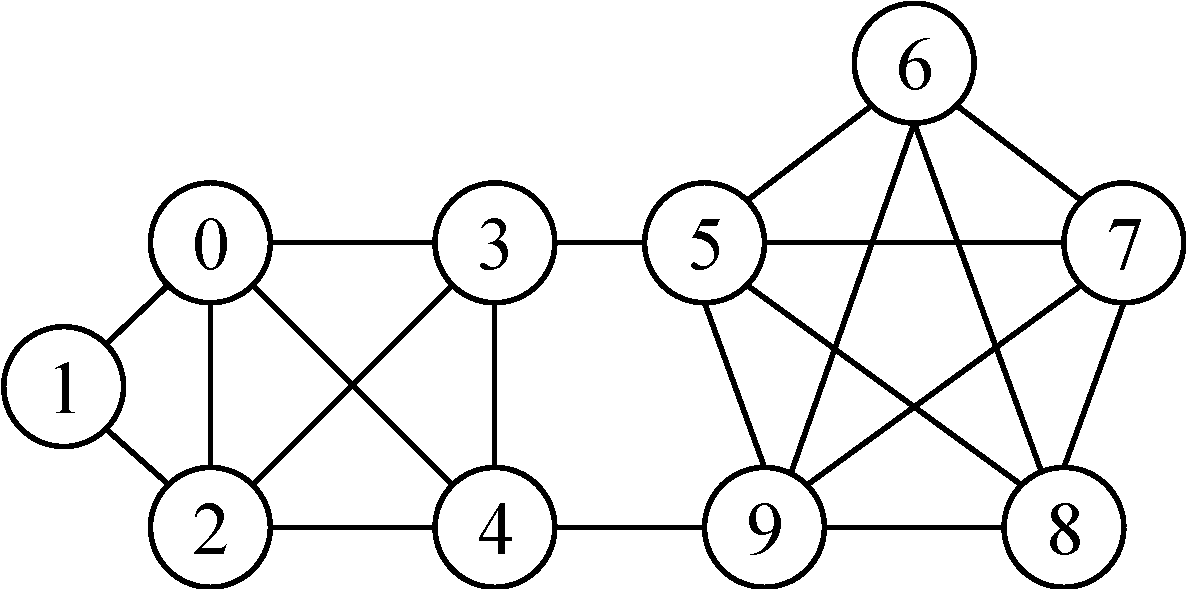
\includegraphics[width=1\linewidth,clip=true]{img/graphs-Graph2.pdf}
    		(a)
    	\end{minipage}
    	\begin{minipage}{0.4\textwidth}
    		\centering
    		\[
	\begin{aligned}[t]
		C_{0} &: 0, 1, 2 \\
		C_{1} &: 0, 2, 3, 4 \\
		C_{2} &: 3, 5 \\
		C_{3} &: 5, 6, 7, 8, 9 \\
		C_{4} &: 4, 9
	\end{aligned}
\]

    		(b)
    	\end{minipage}
    	\begin{minipage}{0.15\textwidth}
    		\centering
    		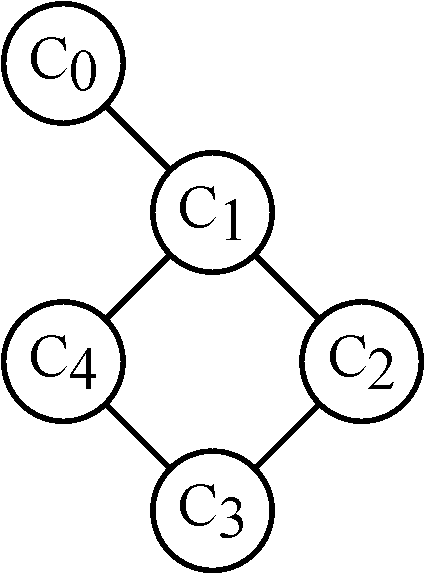
\includegraphics[width=1\linewidth,clip=true]{img/graphs-Cliques2.pdf}
    		(c)
    	\end{minipage}
    \caption{(a) Grafo no dirigido. (b) Lista de cliques maximales. (c) Grafo de cliques.}
    \label{fig:gafoEj}
\end{figure}




\section{Particionamento del grafo de cliques}
Dado que construir el grafo de cliques maximales requiere un tiempo de computación muy alto (necesita el cómputo de intersecciones de conjuntos para todos los pares de cliques maximales), se define una heurística que estima una partición sin calcular el grafo de cliques maximales.
%Teniendo el grafo de cliques maximales, es necesario definir una heurística que permita agruparlos en particiones de manera eficiente, pensando tanto en el espacio que ocuparán las secuencias comprimidas como en tiempos de acceso secuencial y aleatorio.

Se desean encontrar particiones del grafo de cliques que exploten dicha redundancia de vértices en los cliques maximales, y permita agrupar en una misma partición a cliques que tengan una cantidad razonable de vértices en común, y los que no la tengan queden separados en otras particiones. El problema de encontrar particiones de cliques se define a continuación.

\begin{problem}
	\label{def:findPartitions}
	Encontrar particiones de cliques para el grafo de cliques $CG_{\mathcal{C}}$.
	
	Dado un grafo de cliques $CG_{\mathcal{C}} = (V_{\mathcal{C}}, E_{\mathcal{C}})$, encontrar un set de particiones de cliques $\mathcal{C}\mathcal{P} = \{cp_{1}, cp_{2}, ..., cp_{M}\}$ de $CG_{\mathcal{C}}(V_{\mathcal{C}}, E_{\mathcal{C}})$ con $M \geq 1$, tal que
	\begin{enumerate}
		%\item $\bigcup_{i \in \mathcal{C}\mathcal{P}} cp_{i} = CG_{i}$ \label{item:particiones1}
		\item $\bigcup\limits_{i = 1}^{M} cp_{i} = CG_{\mathcal{C}}$ \label{item:particiones1}
		\item $cp_{i} \cap cp_{j} = \varnothing$ para $i \neq j$ \label{item:particiones2}
		\item cualquier $cp_{i} \in \mathcal{C}\mathcal{P}$ es un subgrafo de $CG_{\mathcal{C}}(V_{\mathcal{C}}, E_{\mathcal{C}})$ inducido por el subset de vértices en $cp_{i}$ \label{item:particiones3}
	\end{enumerate}
	
\end{problem}

Esto indica que cada partición es un subgrafo del grafo de cliques maximales del grafo $G(V,E)$. El punto \ref{item:particiones2} es importante, ya que prohíbe que un clique se repita en una partición, no así un subset de vértices de grafo $G(V,E)$ que sí puede estar en varias particiones a la vez.

A continuación se plantea una heurística que, basada en el listado de cliques maximales $\mathcal{C} = \{c_{1}, c_{2}, ..., c_{N} \}$ y funciones de ranking, genere el particionamiento del grafo de cliques sin necesidad de generar dicho grafo.


\section{Algoritmo de particionamiento o clustering} \label{sec:PartitionAlgoritms}

En esta sección se procede a describir el algoritmo para generar las particiones del grafo de cliques. Para ello, en la Definición~\ref{def:rankingFunctions} se define una función de ranking, que valoriza cada vértice según ciertas características. También se detallan ciertas funciones de ranking basadas en la cantidad y tamaño de los cliques maximales donde un vértice se encuentre.

\begin{definition} 
	\label{def:rankingFunctions}
	Función de ranking
	
	Dado un grafo $G = (V, E)$ y $\mathcal{C} = \{c_{1}, c_{2}, ..., c_{N} \}$ el conjunto de tamaño $N$ de cliques maximales que cubren $G$, una función de ranking es una función $r: V \rightarrow \mathbb{R}^{+}$ que retorna un valor de puntuación para cada vértice $v \in V$.
\end{definition}

La heurística de clustering se describe en el Algoritmo~\ref{alg:clustering}. La salida del cálculo de ranking son los arreglos $D$ y $R$ (Algoritmo~\ref{alg:clustering} línea \ref{alg:clustering:rankarray}), donde $D$ contiene los índices de los cliques donde cada vértice participa en el grafo $G$, y $R$ contiene el valor de puntuación para cada vértice en $G$. La complejidad del algoritmo de cálculo de ranking se compone primero por pasar por todos los vértices en $G$ en el conjunto de cliques maximales $\mathcal{C}$, y luego ordenar $R$ de mayor a menor. La complejidad total del algoritmo es de $O(L \log L)$, donde $L=\sum_{c_i \in \mathcal{C}}|c_{i}|$.

Luego se crea un arreglo de bits $Z$ de largo $N = |\mathcal{C}|$ iniciando cada bit en cero, el cual servirá para mantener revisado si un clique ya fue incluido o no en una partición. Se recorre el arreglo $R$ y por cada vértice $u$, se obtienen los índices de los cliques donde $u$ participa según $D[u]$ y se añaden el índice $id$ de cada clique a la partición pertinente ($cpid$) solo si $Z[id] = 0$. Si el índice $id$ fue exitosamente agregado, se cambia el valor de $Z[id] = 1$. Si la partición $cpid$ contiene al menos un índice de clique, la partición es agregada a la colección $\mathcal{C}\mathcal{P}$, y se continúa procesando vértices en $R$. La complejidad del algoritmo para este paso es de $O(N+V)$. Finalmente, el algoritmo retorna la colección de particiones $\mathcal{C}\mathcal{P}$, donde cada partición contiene un set de los índices de cliques que las componen.

\begin{algorithm}
\caption{Algoritmo de particionamiento del grafo de cliques.}
\label{alg:clustering}
\begin{algorithmic}[1]
\REQUIRE $\mathcal{C}$ maximal clique collection ($N=|\mathcal{C}|$), ranking function $r(u)$
\ENSURE Returns clique-graph partition collection $\mathcal{C}\mathcal{P}$
\STATE $(D,R) \leftarrow computeRanking(r,\mathcal{C})$ (array $D$ y $R$, $\forall u \in V$ ) \label{alg:clustering:rankarray} 
\STATE Initialize bit array $Z$ of size $N$ and set each bit to 0
\FOR {$u \in R$}
    \STATE $cpid \leftarrow \emptyset$
     \FOR {$id \in D[u]$ and $D[u]=0$} 
          \STATE $Z[id] \leftarrow 1$
          \STATE $cpid \leftarrow cpid \cup \{id\}$
    \ENDFOR
    \IF {$cpid \neq  \emptyset$}
      \STATE $\mathcal{C}\mathcal{P} \leftarrow \mathcal{C}\mathcal{P} : cpid$
    \ENDIF 
 \ENDFOR
\RETURN $\mathcal{C}\mathcal{P}$
\end{algorithmic}
\end{algorithm}


Las funciones de ranking (Definición~\ref{def:rankingFunctions}) que se proponen toman en cuenta la cantidad y el tamaño de los cliques donde participa cada vértice del grafo $G(V, E)$. Primero se define el conjunto $C(u)$ para cada vértice $u \in V$ como $C(u) = \{c \in \mathcal{C}|u \in c\}$, luego las funciones de rankings son las siguientes:

\begin{align}
	r_{f}(u) &= |C(u)| \label{eq:rankFunF}  \\ 
	r_{c}(u) &= \sum_{c \in C(u)}|c| \label{eq:rankFunC} \\ 
	r_{r}(u) &= \frac{r_{c}(u)}{r_{f}(u)} \label{eq:rankFunR}
\end{align}


La función $r_{f}(u)$ (\autoref{eq:rankFunF}) indica en cuántos cliques está presente el vértice $u$, la función $r_{c}(u)$ (\autoref{eq:rankFunC}) entrega la suma del tamaño de los cliques donde está presente el vértice $u$, y la función $r_{r}(u)$ (\autoref{eq:rankFunR}) es la razón entre $r_{c}(u)$ y $r_{f}(u)$. En la \autoref{fig:sequences} se muestra el resultado de las funciones de ranking para el caso ejemplo, y las particiones de cliques resultantes para cada una.

\begin{figure}
    \centering

    \begin{minipage}{\textwidth}
    	\centering
    	\begin{tabular}{c|c|c|c|c|c|c|c|c|c|c|}
	\cline{2-11}
	$u \in G$ & 0 & 1 & 2 & 3 & 4 & 5 & 6 & 7 & 8 & 9 \\
	\cline{2-11}
	$R_{rf}$ & 2,0 & 1,0 & 2,0 & 2,0 & 2,0 & 1,0 & 1,0 & 1,0 & 1,0 & 2,0 \\
	\cline{2-11}
	$R_{rc}$ & 7,0 & 3,0 & 7,0 & 6,0 & 6,0 & 7,0 & 5,0 & 5,0 & 5,0 & 7,0 \\
	\cline{2-11}
	$R_{rr}$ & 3,5 & 3,0 & 3,5 & 3,0 & 3,0 & 3,5 & 5,0 & 5,0 & 5,0 & 3,5 \\
    \cline{2-11}
\end{tabular}

    	
    	(a)
    \end{minipage}

    \hfill\vline\hfill
    
    \begin{minipage}{\textwidth}
    	\centering
    	\begin{tabular}{c|c|c|c|c|}
	\cline{2-5}
	$\mathcal{C}\mathcal{P}_{rf}$ & $C_{0} \quad C_{1}$ & $C_{2}$ & $C_{4}$ & $C_{3}$ \\
	\cline{2-5}
	$\mathcal{C}\mathcal{P}_{rc}$ & $C_{0} \quad C_{1}$ & $C_{2} \quad C_{3}$ & $C_{4}$ \\
	\cline{2-5}
	$\mathcal{C}\mathcal{P}_{rr}$ & $C_{3}$ & $C_{0} \quad C_{1}$ & $C_{2}$ & $C_{4}$ \\
	\cline{2-5}
\end{tabular}

    	
    	(b)
    \end{minipage}
    
    \caption{Resultados de las funciones de ranking, asociados al grafo de la \autoref{fig:gafoEj}. (a) Puntaje final. (b) Particiones de cliques.}
    \label{fig:sequences}
\end{figure}


\section{Representación en estructuras compactas}

En esta sección se detalla la estructura compacta para representar $G(V, E)$ usando las particiones $\mathcal{C}\mathcal{P}$ obtenida en la \autoref{sec:PartitionAlgoritms}. Se consideran estructuras de datos compactas  basadas en símbolos y secuencias de bits, con soporte para las operaciones de \textit{rank()}, \textit{select()} y \textit{access()}.

\subsection{Secuencias de la representación de las particiones}
La representación de las particiones consta de cuatro elementos, dos secuencias de enteros \textbf{X} e \textbf{Y}, un mapa de bits \textbf{B}, y una secuencia de bytes \textbf{BB}, las cuales se describen a continuación.

\begin{itemize}
	\item La secuencia de enteros \textbf{X} consiste en las listas concatenadas de los vértices presentes en los cliques de cada partición.
	\item El mapa de bits \textbf{B} contiene un bit por cada elemento en \textbf{X} inicializados en cero, indicando el inicio de las particiones con un uno. Además se agrega un bit extra en uno al final de la secuencia para indicar su final.
	\item La secuencia de bytes \textbf{BB} codifica en qué cliques está presente cada vértice, marcando un  $1$ en cada bit de cada byte por clique si el vértice pertenece a ese clique.
	\item La secuencia de enteros \textbf{Y} indica cuántos bytes omitir en \textbf{BB} para acceder rápidamente a la partición deseada.
\end{itemize}

La definición formal de la estructura se presenta en la Definición~\ref{def:sequences}. Se puede observar en la \autoref{eq:bbp} que $BB_{p} \in BB$ es una matriz de bytes, donde cada fila representa un vértice $u$ en $X_{p} \in X$, y las columnas corresponden a los bytes usados por los vértices para marcar los cliques donde participan en la partición. 

También se debe notar el caso especial, cuando un clique maximal queda solo en una partición, no ocupa espacio en su $BB_{p}$ correspondiente. Para poder reconocer estos casos, se agrupan al final de la estructura compacta todas estas particiones, y con esto se puede ahorrar espacio tanto en $BB$ como en $Y$.

\begin{definition} 
	\label{def:sequences}
	Representación compacta del grafo $G(V, E)$. 
	
	Dado $\mathcal{C}\mathcal{P} = \{cp_{0},...,cp_{M-1}\}$, $cp_{p} \in \mathcal{C}\mathcal{P}$, y $cp_{p}=\{c_{0},...,c_{m_{r}-1}\}$. 
	Se especifica $bpu_{p} = \ceil*{\frac{m_{r}-1}{8}}$ como la cantidad de bytes por vértice $u$ en $X_{p}$, y se definen las secuencias $X_{p}$, $B_{p}$, $BB_{p}$, $Y_{p}$ como sigue:
	
	\begin{align}
		X_{p} &= \{u \in c|c \in cp_{p}\} = \{u_{0},...u_{|X_{p}|-1}\} \\
		B_{p} &= 1:0^{|X_{p}|-1} \\
		BB_{p} &= bb[|X_{p}|][bpu_{p}]   \label{eq:bbp} \\
		bb[i][j] &= \begin{cases}
                  \sum_{k=0}^{7} 2^{k}(u_{i} \in c_{8j+k}), & bpu_{p} \neq 0  \\
                  %, & x \in c , x \in X_{p}, c \in OC_{r} \\
                  \emptyset, & otherwise \\
                 \end{cases} \nonumber \\
		Y_{p} &= \begin{cases}
				|X_{p}|\times bpu_{p} + Y_{p-1}, & bpu_{p} \neq 0  \\
				 \emptyset, & otherwise \\
			\end{cases}
	\end{align}
\end{definition}

%\textcolor{red}{Cambié la definición de Y, para dejar en claro que si una partición no tiene bytes en BB, tampoco tendrá un Y asociado.}

En la \autoref{fig:compactStructure} se presenta la estructura resultante del ejemplo, usando las particiones $\mathcal{C}\mathcal{P}_{rr}$ reordenadas. Como se puede apreciar, solo la primera partición tiene dos cliques, por tanto será la única que agregue bytes en la secuencia $BB$, codificando la pertenencia de cada clique en un bit del byte, requiriendo entonces solo un byte por vértice en $X$.

Cada secuencia $X_{p}$ consiste en la unión de los vértices que comparten todos los cliques de en la partición $p$. La secuencia $X$ está formada por la concatenación de todas las secuencias $X_{p}$. La secuencia $B$ escribe un 1 en cada inicio de una partición más uno extra para indicar el final. Para la secuencia $BB$, los cliques involucrados son $C_{0}: \{0, 1, 2\}$ y $C_{1}: \{0, 2, 3, 4\}$, ambos contienen los vértices $0$ y $2$, codificado con sus bytes en $3$, el vértice $1$ solo está presente en $C_{0}$ y se codifica con su respectivo byte en $1$, y los vértices $3$ y $4$ solo participan en $C_{1}$ y sus bytes toman el valor $2$. Finalmente la secuencia $Y$ se inicia con un  5 por la cantidad de cliques presentes en la primera partición, y como las siguientes solo tienen un clique, no se agregan más enteros.
%La secuencia $X$ se conforma por todos los vértices que conforman los cliques en cada partición, ordenados de menor a mayor. La secuencia $B$ escribe un 1 en cada inicio de una partición más uno extra para indicar el final. Para la secuencia $BB$, los cliques involucrados son $C_{0}: \{0, 1, 2\}$ y $C_{1}: \{0, 2, 3, 4\}$, ambos contienen los vértices $0$ y $2$, codificado con sus bytes en $3$, el vértice $1$ solo está presente en $C_{0}$ y se codifica con su respectivo byte en $1$, y los vértices $3$ y $4$ solo participan en $C_{1}$ y sus bytes toman el valor $2$. Finalmente la secuencia $Y$ se inicia con un  5 por la cantidad de cliques presentes en la primera partición, y como las siguientes solo tienen un clique, no se agregan más enteros.

\begin{figure}
	\centering
	\begin{minipage}{0.45\textwidth}
		\centering
		\begin{tabular}{c|c|c|c|c|}
	\cline{2-5}
	$\mathcal{C}\mathcal{P}_{rr}$ &  $C_{0} \quad C_{1}$ & $C_{3}$ & $C_{2}$ & $C_{4}$ \\
	\cline{2-5}
\end{tabular}

	
		(a)
	\end{minipage}
	\begin{minipage}{0.45\textwidth}
		\centering
		\begin{tabular}{c|c|c|c|c|c|c|c|c|c|c|c|c|c|c|c|}
	\cline{2-15}
	$X$: & 0 & 1 & 2 & 3 & 4 & 5 & 6 & 7 & 8 & 9 & 3 & 5 & 4 & 9 \\
	\cline{2-16}
	$B$: & 1 & 0 & 0 & 0 & 0 & 1 & 0 & 0 & 0 & 0 & 1 & 0 & 1 & 0 & 1 \\
	\cline{2-16}
	$BB$: & 3 & 1 & 3 & 2 & 2 \\
	\cline{2-6}
	$Y$: & 0 & 5 \\
	\cline{2-3}
\end{tabular}

		
		(b)
	\end{minipage}
	
	\caption{Ejemplo de reordenamiento y estructura compacta. (a) $\mathcal{C}\mathcal{P}_{rr}$ reordenado. (b) Estructura compacta reordenada.}
	\label{fig:compactStructure}
\end{figure}



\subsection{Algoritmos de consulta}
A continuación se presentan los algoritmos de consulta que soporta la estructura compacta. El Algoritmo~\ref{alg:sequential} reconstruye el grafo $G(V, E)$ recorriendo de manera secuencial la estructura compacta. El Algoritmo~\ref{alg:neighbors} recupera el listado de vecinos para un vértice cualquiera $u$ del grafo $G(V, E)$. El Algoritmo \ref{alg:twonodes} verifica si dos vértices son vecinos. El Algoritmo~\ref{alg:cliques} recupera el listado de cliques maximales $\mathcal{C}$ del grafo $G(V, E)$.

Para reconstruir el grafo, el Algoritmo~\ref{alg:sequential} recorre secuencialmente la estructura compacta, revisando los vecinos de cada partición. Si una partición contiene un solo clique entonces todos los vértices asociados son vecinos. Si contiene más de un clique, para cada vértice en $X$ se comparan sus bytes asociados en $BB$ con todos los demás, y si el resultado es distinto de cero, son vecinos. La cantidad de cliques se determina rápidamente al comparar el valor de la secuencia $Y$ de cada partición con la anterior; si es el mismo valor significa que hay un solo clique, si cambió es que hay más de uno.

Primero obtiene la cantidad $P$ de particiones, contando la cantidad de unos en la secuencia $B$. Para cada una de las particiones, se obtiene el índice del inicio ($s$) y final ($e$) de la partición en la secuencia $B$. Luego se calcula en $bpu_{p}$ la cantidad de bytes por vértice en la secuencia $X$, y se copia el listado de vértices de la partición actual a RAM para mejorar el tiempo de acceso. Por cada vértice, se revisan los demás restantes; si la cantidad de bytes por vértice es cero, se agregan todos los pares de vértices a la reconstrucción del grafo. De lo contrario, se comparan todos los bytes por vértice correspondientes, y si dicha comparación da algo distinto a cero, se agrega esa arista a ambos vértices involucrados, y se continúa con el siguiente vértice. Cuando se revisan todas las combinaciones de pares de vértices posibles, se prosigue con la partición siguiente. Finalmente retorna el grafo completo $G$.  La complejidad de este algoritmo es $O(P_{0} \cdot N^{2})$ cuando $bpu_{p}$ es igual a cero, de lo contrario $O(P_{1} \cdot N^{2} \cdot bpu_{p})$, siendo $P_{0}$ el número de particiones con cero bytes por vértice, $P_{1}$ las particiones que sí tienen bytes por vértice, y $N$ el largo de las particiones.

Para encontrar vecinos de vértices aleatorios, el Algoritmo~\ref{alg:neighbors}) detecta las particiones donde participa el vértice $u$ en la secuencia $X$, y luego revisa cada partición detectada. Gracias a las funciones de acceso \textit{rank()}, \textit{select()} y \textit{access()} que soporta la estructura compacta, esta tarea se realiza de manera eficiente.

Primero se cuentan las ocurrencias del vértice $u$, y por cada una se obtiene el inicio y final de las particiones donde está presente, junto con la cantidad de bytes por vértice y la copia a RAM de los vértices que tiene dicha partición. Luego, por cada vértice en la partición y posible vecino, si $bpu_{p}$ es cero se agrega directamente dicho vértice al listado de vecinos de $u$. Si no lo es, se comparan uno a uno los bytes por vértice de $u$ con su posible vecino, y si alguna comparación es distinta de cero, se agrega el vértice en evaluación al listado final y se continúa al siguiente posible. Finalmente retorna el listado de vecinos $N(u)$. La complejidad del algoritmo es $O(M_{0} \cdot N)$ cuando $bpu_{p}$ es igual a cero, y $O(M_{1} \cdot N \cdot bpu_{p})$ cuando no lo es, siendo $M_{0}$ la cantidad de particiones que contienen al vértice en la secuencia $X$ con cero bytes por vértice, $M_{1}$ el resto de particiones con bytes por vértice distinto de cero, y $N$ el largo de las particiones.

Para verificar si dos vértices son vecinos, el Algoritmo~\ref{alg:twonodes}  primero cuenta las ocurrencias de ambos nodos en la secuencia $X$, y luego revisa de manera ordenada en qué particiones se encuentra cada una de ellas. Si dos ocurrencias coinciden en una partición, revisa si existe algún bit en común entre sus correspondientes bytes de $BB$, si lo hay entonces son vecinos, de lo contrario continúa buscando otra partición donde vuelvan a encontrarse ambos nodos. La complejidad del algoritmo es $O(M_{1} + M_{2})$ cuando $bpu_{p}$ es igual a cero, y $O((M_{1} + M_{2}) \cdot bpu_{p})$ cuando no lo es, siendo $M_{1}$ el número de particiones que contienen al vértice $u_{1}$, y $M_{2}$ el número de particiones que contienen al vértice $u_{2}$.

Para recuperar el listado de cliques maximales, el Algoritmo~\ref{alg:cliques} recorre la estructura compacta de manera secuencial, y va recreando los cliques representados por los bytes en la secuencia $BB$ de cada partición.

El algoritmo primero obtiene la cantidad de particiones $P$, luego por cada una de ellas obtiene sus índices de inicio ($s$) y final ($e$) en $B$, calcula la cantidad de bytes por vértice $bpu_{p}$, y copia a RAM los vértices de la partición. Si $bpu_{p}$ es cero, quiere decir que todos los vértices pertenecen al mismo clique, por tanto los agrega como un clique directamente. Y si $bpu_{p}$ es distinto de cero, revisa por cada vértice y cada bit de cada byte la pertenencia de dicho vértice a un clique maximal; si el bit es uno lo agrega, y si es cero lo omite. Finalmente, agrega cada clique detectado al listado final de cliques maximales. La complejidad del algoritmo es $O(P_{0} \cdot N)$ cuando $bpu_{p}$ es igual a cero, y $O(P_{1} \cdot N \cdot 8 \cdot bpu_{p})$ cuando no lo es, siendo $P_{0}$ el número de particiones con cero bytes por vértice, $P_{1}$ las particiones que sí tienen bytes por vértice, y $N$ el largo de las particiones.

%\textcolor{red}{Las notaciones de complejidad de los algoritmos me causan duda, separando siempre cuando hay o no bytes en BB.}
%\textcolor{red}{Por favor revisar el algoritmo de consulta si dos nodos son vecinos. Además, realicé algunos cambios menores en los demás algoritmos, por favor revisar igual.}

\begin{algorithm}[H]
\caption{Algoritmo secuencial para reconstruir $G(V, E)$.}
\caption{Algoritmo secuencial para reconstruir $G(V, E)$.}
\label{alg:sequential}
\begin{algorithmic}[1]
    \REQUIRE $X$, $B$, $BB$, $Y$
    \ENSURE Returns $G(V, E)$

    \STATE Initialize empty graph $G$
    \STATE $P \leftarrow rank_{1}(B,|B|)$

    \FOR {$p = 1$ \TO $P$}
    	\STATE $s \leftarrow select_{1}(B, p)$
    	\STATE $e \leftarrow select_{1}(B, p + 1)$
        \STATE $bpu_{p} \leftarrow \frac{Y_{p + 1} - Y_{p}}{e - s}$
        \STATE $X_{p} \leftarrow X[s..e]$

        \FOR{$j = 0$ \TO $|X_{p}|$}
            \FOR{$k = j + 1$ \TO $|X_{p}|$}
            
            		\IF{$bpu_{p} = 0$}
                		\STATE Insert (unoriented) edges $(X_{p}[j], X_{p}[k])$ into $G$
                	\ELSE
                		\FOR{$b = 1$ \TO $bpu_{p}$}
                    		\IF {$BB_{p}[bpu_{p} \cdot j + b]$ \& $BB_{p}[bpu_{p} \cdot k + b] \neq 0$}
                        		\STATE Insert (unoriented) edge $(X_{p}[j], X_{p}[k])$ into $G$
                        		\STATE $break$
                    		\ENDIF
                		\ENDFOR
                	\ENDIF
                	
            \ENDFOR
        \ENDFOR
       
   	\ENDFOR 
    \RETURN $G$
\end{algorithmic}
\end{algorithm}


\begin{algorithm}[H]
\caption{Algoritmo para recuperar vecinos $N(u)$ de un vértice $u \in V$.}
\label{alg:neighbors}
\begin{algorithmic}[1]
    \REQUIRE $u$, $X$, $B$, $BB$, $Y$
    \ENSURE Returns $N(u)$

    \STATE Initialize empty graph $N(u)$
    \STATE $occur \leftarrow rank_{u}(X, |X|)$

    \FOR {$i = 1$ \TO $occur$}
        	\STATE $u_{p} \leftarrow select_{u}(X, i)$
        	\STATE $p \leftarrow rank_{1}(B, u_{p})$
        	\STATE $s \leftarrow select_{1}(B, p)$
    		\STATE $e \leftarrow select_{1}(B, p + 1)$
        	\STATE $bpu_{p} \leftarrow \frac{Y_{p + 1} - Y_{p}}{e - s}$
        	\STATE $X_{p} \leftarrow X[s..e]$

        	\FOR{$j = 0$ \TO $|X_{p}|$}
       		\IF{$X_{p}[j] \neq u$}
       		
       			\IF{$bpu_{p} = 0$}
            			\STATE Insert $X_{p}[j] \neq u$ to $N(u)$
            		\ELSE
                		\STATE $BB_{p} \leftarrow \mathit{HuffmanToBytes}(BB[Y_{p}], BB[Y_{p + 1}])$
                		\STATE $iBBj \leftarrow bpu_{p} \cdot j$
                		\STATE $iBBx \leftarrow bpu_{p} \cdot (u_{p} - s)$
                		
            			\FOR{$b = 1$ \TO $bpu_{p}$}
                			\IF {$BB_{p}[iBBx + b]$ \& $BB_{p}[iBBj + b] \neq 0$}
                    			\STATE Insert $X_{p}[j]$ into $N(u)$
                    			\STATE $break$
                			\ENDIF
            			\ENDFOR
            		\ENDIF
            		
            	\ENDIF
        \ENDFOR
    \ENDFOR

    \RETURN $N(u)$
\end{algorithmic}
\end{algorithm}


\begin{algorithm}[H]
\caption{Algoritmo para verificar si dos nodos $u_{1}, u_{2} \in V$ son vecinos.}
\label{alg:twonodes}
\begin{algorithmic}[1]
    \REQUIRE $u_{1}$, $u_{2}$, $X$, $B$, $BB$, $Y$
    \ENSURE Returns if $(u_{1}, u_{2}) \in E$

    \STATE $occur_{1} \leftarrow rank_{u_{1}}(X, |X|)$
    \STATE $occur_{2} \leftarrow rank_{u_{2}}(X, |X|)$
    
    \STATE $ySize \leftarrow |Y|$
    
    \STATE $u1_{p} \leftarrow select_{u_{1}}(X, 1)$
    	\STATE $p1 \leftarrow rank_{1}(B, u1_{p})$
    	\STATE $i1 \leftarrow 1$

    \FOR {$i2 = 1$ \TO $occur_{2}$}
        	\STATE $u2_{p} \leftarrow select_{u_{2}}(X, i2)$
        	\STATE $p2 \leftarrow rank_{1}(B, u2_{p})$
        	
        	\WHILE {$p1 < p2$}
        		\STATE $i1 \leftarrow i1 + 1$
        		\IF {$i1 > occur_{1}$}
        			\RETURN \FALSE
        		\ENDIF
        		\STATE $u1_{p} \leftarrow select_{u_{1}}(X, i1)$
    			\STATE $p1 \leftarrow rank_{1}(B, u1_{p})$
    		\ENDWHILE
    		
    		\IF {$p1 = p2$}
    			\IF {$ySize < p1$}
    				\RETURN \TRUE
    			\ENDIF
    			
    			\STATE $s \leftarrow select_{1}(B, p1)$
    			\STATE $e \leftarrow select_{1}(B, p1 + 1)$
        		\STATE $bpu_{p} \leftarrow \frac{Y_{p1 + 1} - Y_{p1}}{e - s}$
             \STATE $BB_{p} \leftarrow \mathit{HuffmanToBytes}(BB[Y_{p}], BB[Y_{p + 1}])$
             
			\STATE $iBB1 \leftarrow bpu_{p}  \cdot (u1_{p} - s)$
			\STATE $iBB2 \leftarrow bpu_{p} \cdot (u2_{p} - s)$
        		
			\FOR{$b = 1$ \TO $bpu_{p}$}
                	\IF {$BB_{p}[iBB1 + b]$ \& $BB_{p}[iBB2 + b] \neq 0$}
                		\RETURN \TRUE
                	\ENDIF
            	\ENDFOR        		
        		
    		\ENDIF
        
    \ENDFOR

    \RETURN $\FALSE$
\end{algorithmic}
\end{algorithm}


\begin{algorithm}[H]
\caption{Algoritmo para recuperar listado de cliques maximales $\mathcal{C}$ de $G(V, E)$.}
\label{alg:cliques}
\begin{algorithmic}[1]
    \REQUIRE $X$, $B$, $BB$, $Y$
    \ENSURE Returns collection of maximal cliques $\mathcal{C}$

    \STATE $\mathcal{C} \leftarrow \emptyset$
    \STATE $P \leftarrow rank_{1}(B, |B|)$

    \FOR {$p = 1$ \TO $P$}
        \STATE $s \leftarrow select_{1}(B, p)$
        \STATE $e \leftarrow select_{1}(B, p + 1)$
        \STATE $bpu_{p} \leftarrow \frac{Y_{p + 1} - Y_{p}}{e - s}$
        \STATE $X_{p} \leftarrow X[s..e]$
        
        \IF {$bpu_{p} = 0$}
            \STATE $\mathcal{C} \leftarrow \mathcal{C} \cup {X_{p}[e..s]}$
       	\ELSE
       		\STATE $BB_{p} \leftarrow \mathit{HuffmanToBytes}(BB[Y_{p}], BB[Y_{p + 1}])$

		\STATE $CC \leftarrow \emptyset$
        	\FOR{$j = 0$ \TO $|X_{p}| - 1$}
            	\STATE $cluster \leftarrow 0$
            	\STATE $iBBj \leftarrow bpu_{p} \cdot j$
            	
            	\FOR{$b = 1$ \TO $bpu_{p}$}

                	\FOR{$k = 1$ \TO $8$}
                		\STATE $CC[cluster] \leftarrow \emptyset$
                    	%\IF {($BBr[bpup*j+b]$ and $BBr[bpup*k+b]$)}
                    	\IF {$BB_{p}[iBBj + b][k] = 1$}
                        	%\STATE Insert vertex $X_{p}[j]$ to $C[cluster]$
                        	\STATE $CC[cluster] \leftarrow CC[cluster] \cup X_{p}[j]$
                    	\ENDIF
                    	\STATE $cluster \leftarrow cluster + 1$
                	\ENDFOR
                	
            	\ENDFOR
        	\ENDFOR
        \ENDIF
        
        \STATE $\mathcal{C} \leftarrow \mathcal{C} \cup \{CC[1], CC[2], \cdots, CC[cluster]\}$
    \ENDFOR

    \RETURN $\mathcal{C}$
\end{algorithmic}
\end{algorithm}




%% Cliques
\begin{frame}
\frametitle{Resultados - Distribución de tamaño de cliques}

\begin{figure}
    \centering
    	\begin{minipage}{1\textwidth}
    		\centering
    		\begin{minipage}{0.45\textwidth}
    			\centering
    			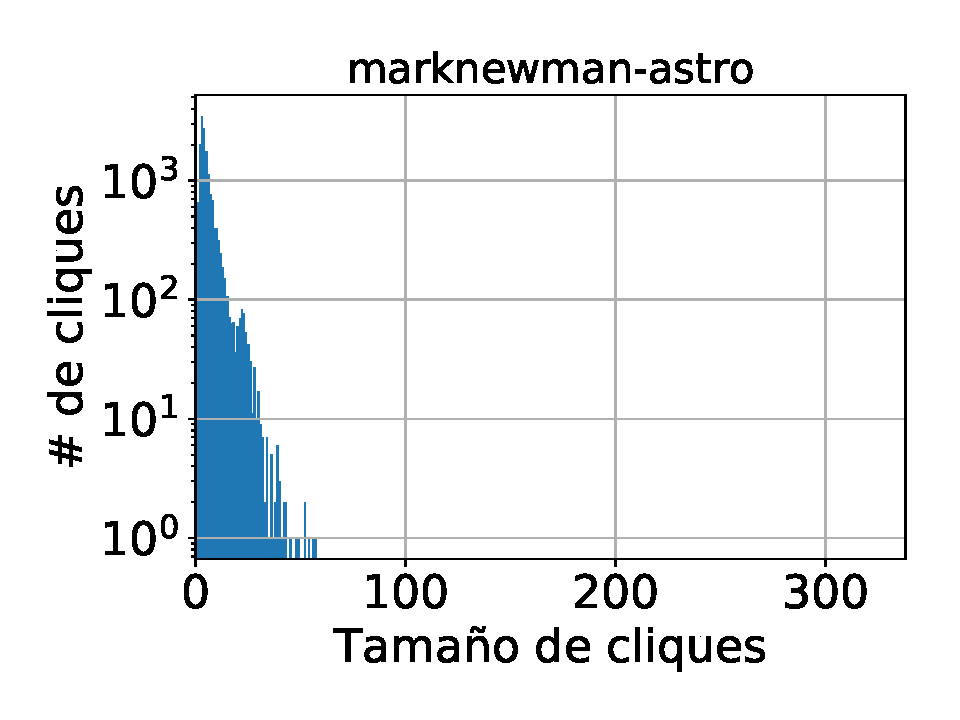
\includegraphics[width=1\linewidth]{../img/cliqueDist2/marknewman-astro.pdf}
    		\end{minipage}
    		\begin{minipage}{0.45\textwidth}
    			\centering
    			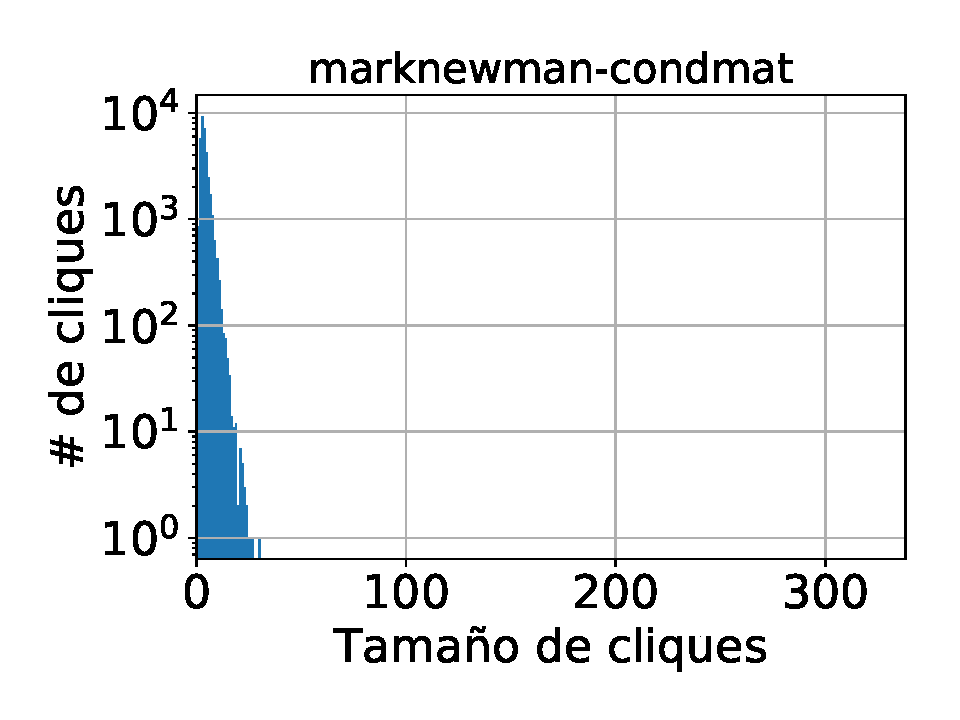
\includegraphics[width=1\linewidth]{../img/cliqueDist2/marknewman-condmat.pdf}
    		\end{minipage}  		
    	\end{minipage}
    	
    	\begin{minipage}{1\textwidth}
    		\centering
    		\begin{minipage}{0.45\textwidth}
    			\centering
    			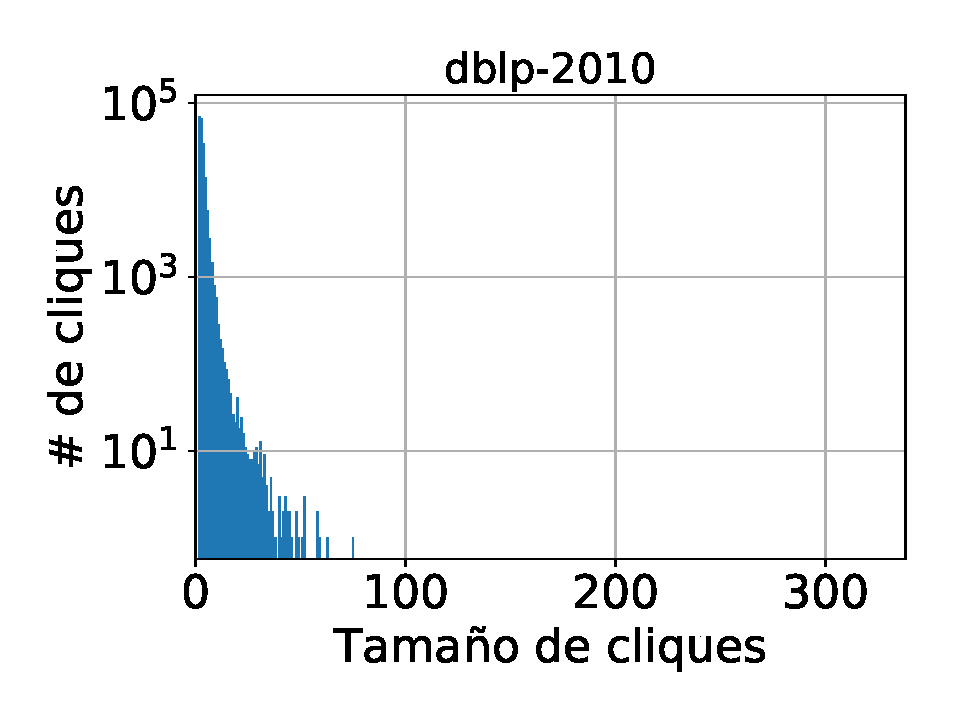
\includegraphics[width=1\linewidth]{../img/cliqueDist2/dblp-2010.pdf}
    		\end{minipage}
    		\begin{minipage}{0.45\textwidth}
    			\centering
    			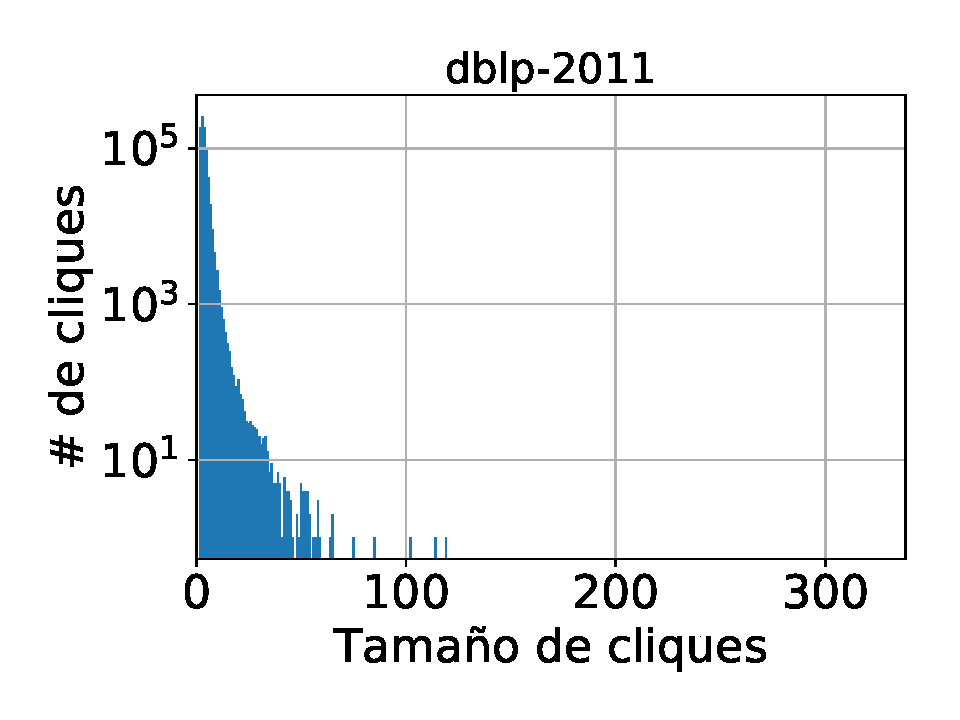
\includegraphics[width=1\linewidth]{../img/cliqueDist2/dblp-2011.pdf}
    		\end{minipage}  
    	\end{minipage}	

    \caption{Distribución del grado de los vértices para cada grafo (1).}
\end{figure}



\end{frame}
\begin{frame}%[noframenumbering]
\frametitle{Resultados - Distribución de tamaño de cliques}

\begin{figure}
    \centering
    	\begin{minipage}{1\textwidth}
    		\centering
    		\begin{minipage}{0.45\textwidth}
    			\centering
    			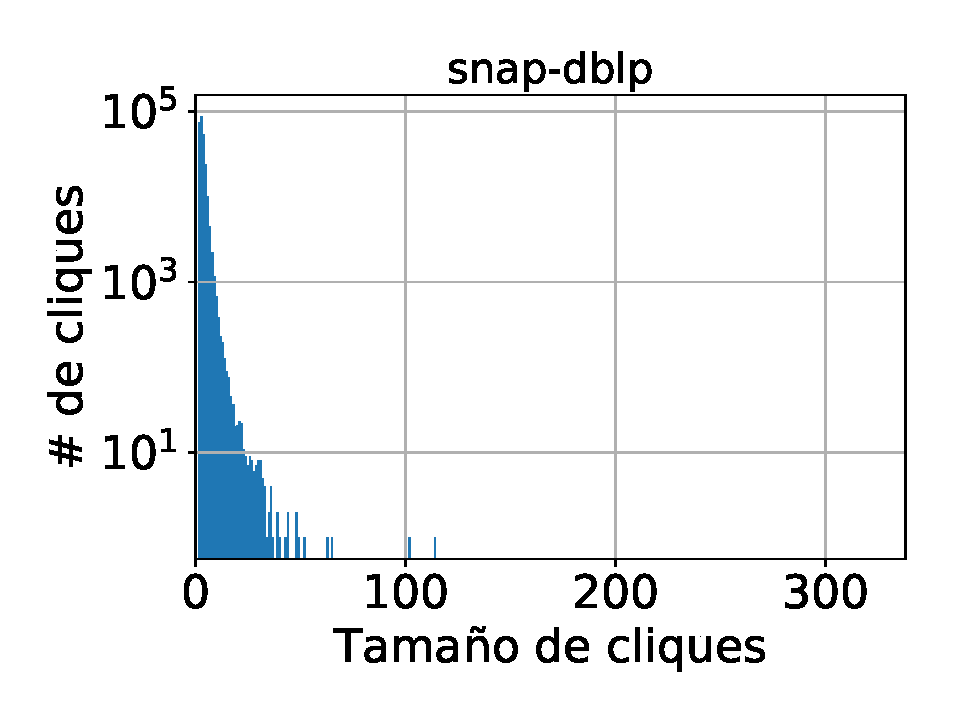
\includegraphics[width=1\linewidth]{../img/cliqueDist2/snap-dblp.pdf}
    		\end{minipage}
    		\begin{minipage}{0.45\textwidth}
    			\centering
    			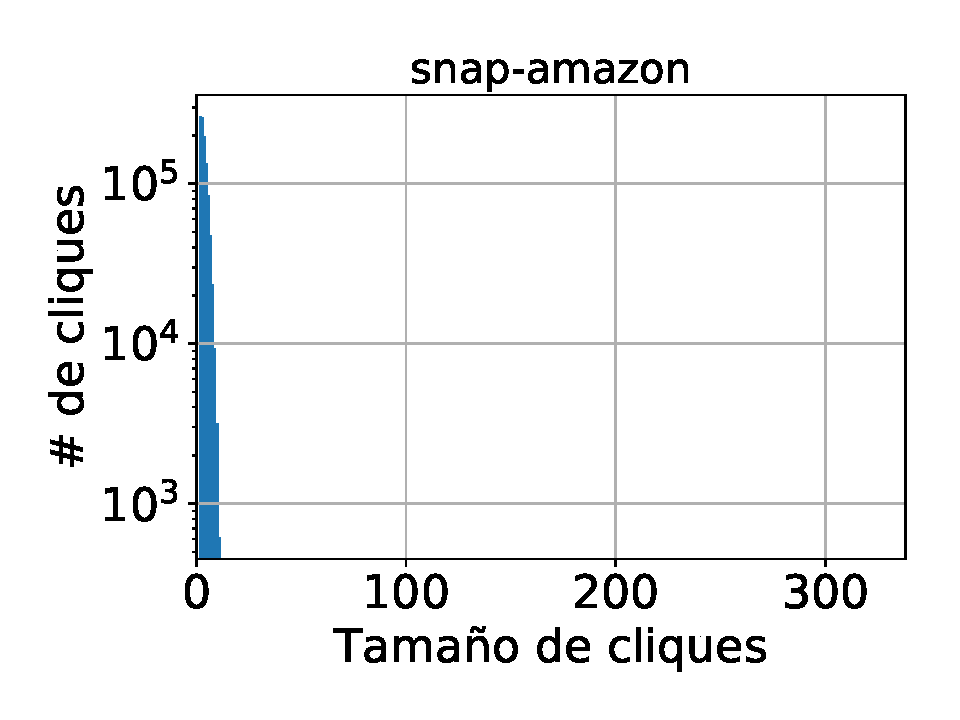
\includegraphics[width=1\linewidth]{../img/cliqueDist2/snap-amazon.pdf}
    		\end{minipage}  		
    	\end{minipage}
    	
    	\begin{minipage}{1\textwidth}
    		\centering
    		\begin{minipage}{0.45\textwidth}
    			\centering
    			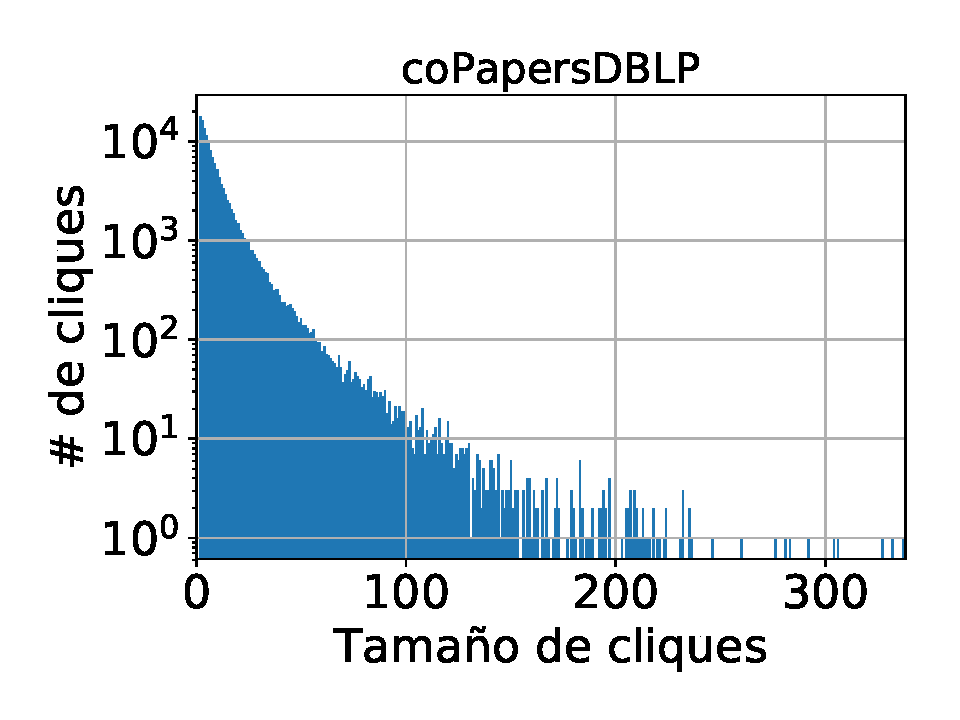
\includegraphics[width=1\linewidth]{../img/cliqueDist2/coPapersDBLP.pdf}
    		\end{minipage}
    		\begin{minipage}{0.45\textwidth}
    			\centering
    			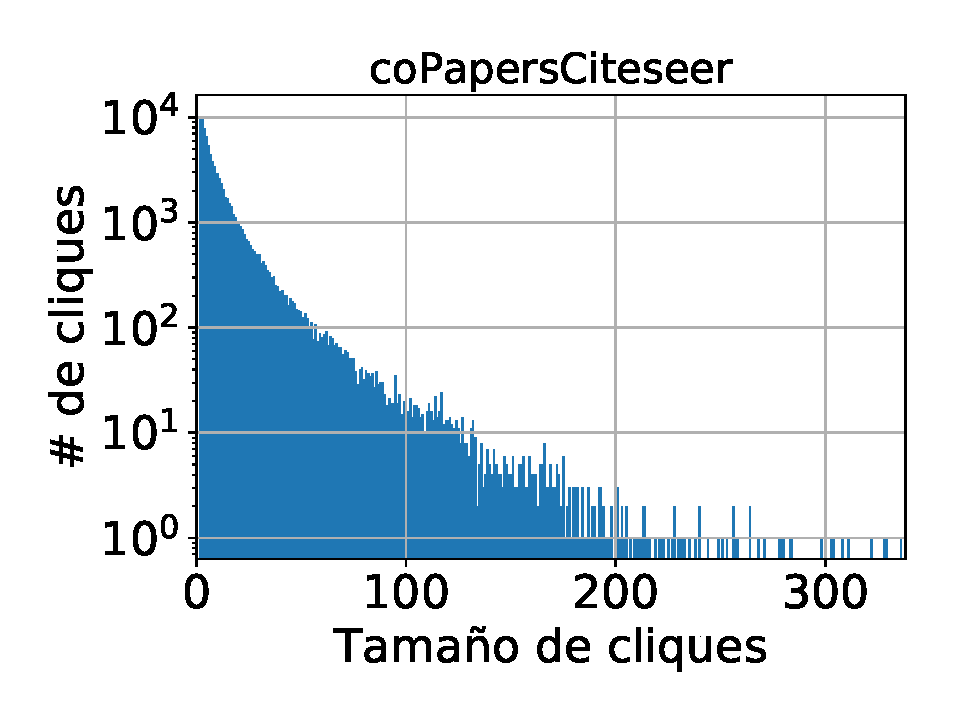
\includegraphics[width=1\linewidth]{../img/cliqueDist2/coPapersCiteseer.pdf}
    		\end{minipage}  
    	\end{minipage}	

    \caption{Distribución del grado de los vértices para cada grafo (2).}
\end{figure}

\end{frame}



\begin{frame}
\frametitle{Resultados - Funciones de ranking}

\begin{figure}
    	\centering
    	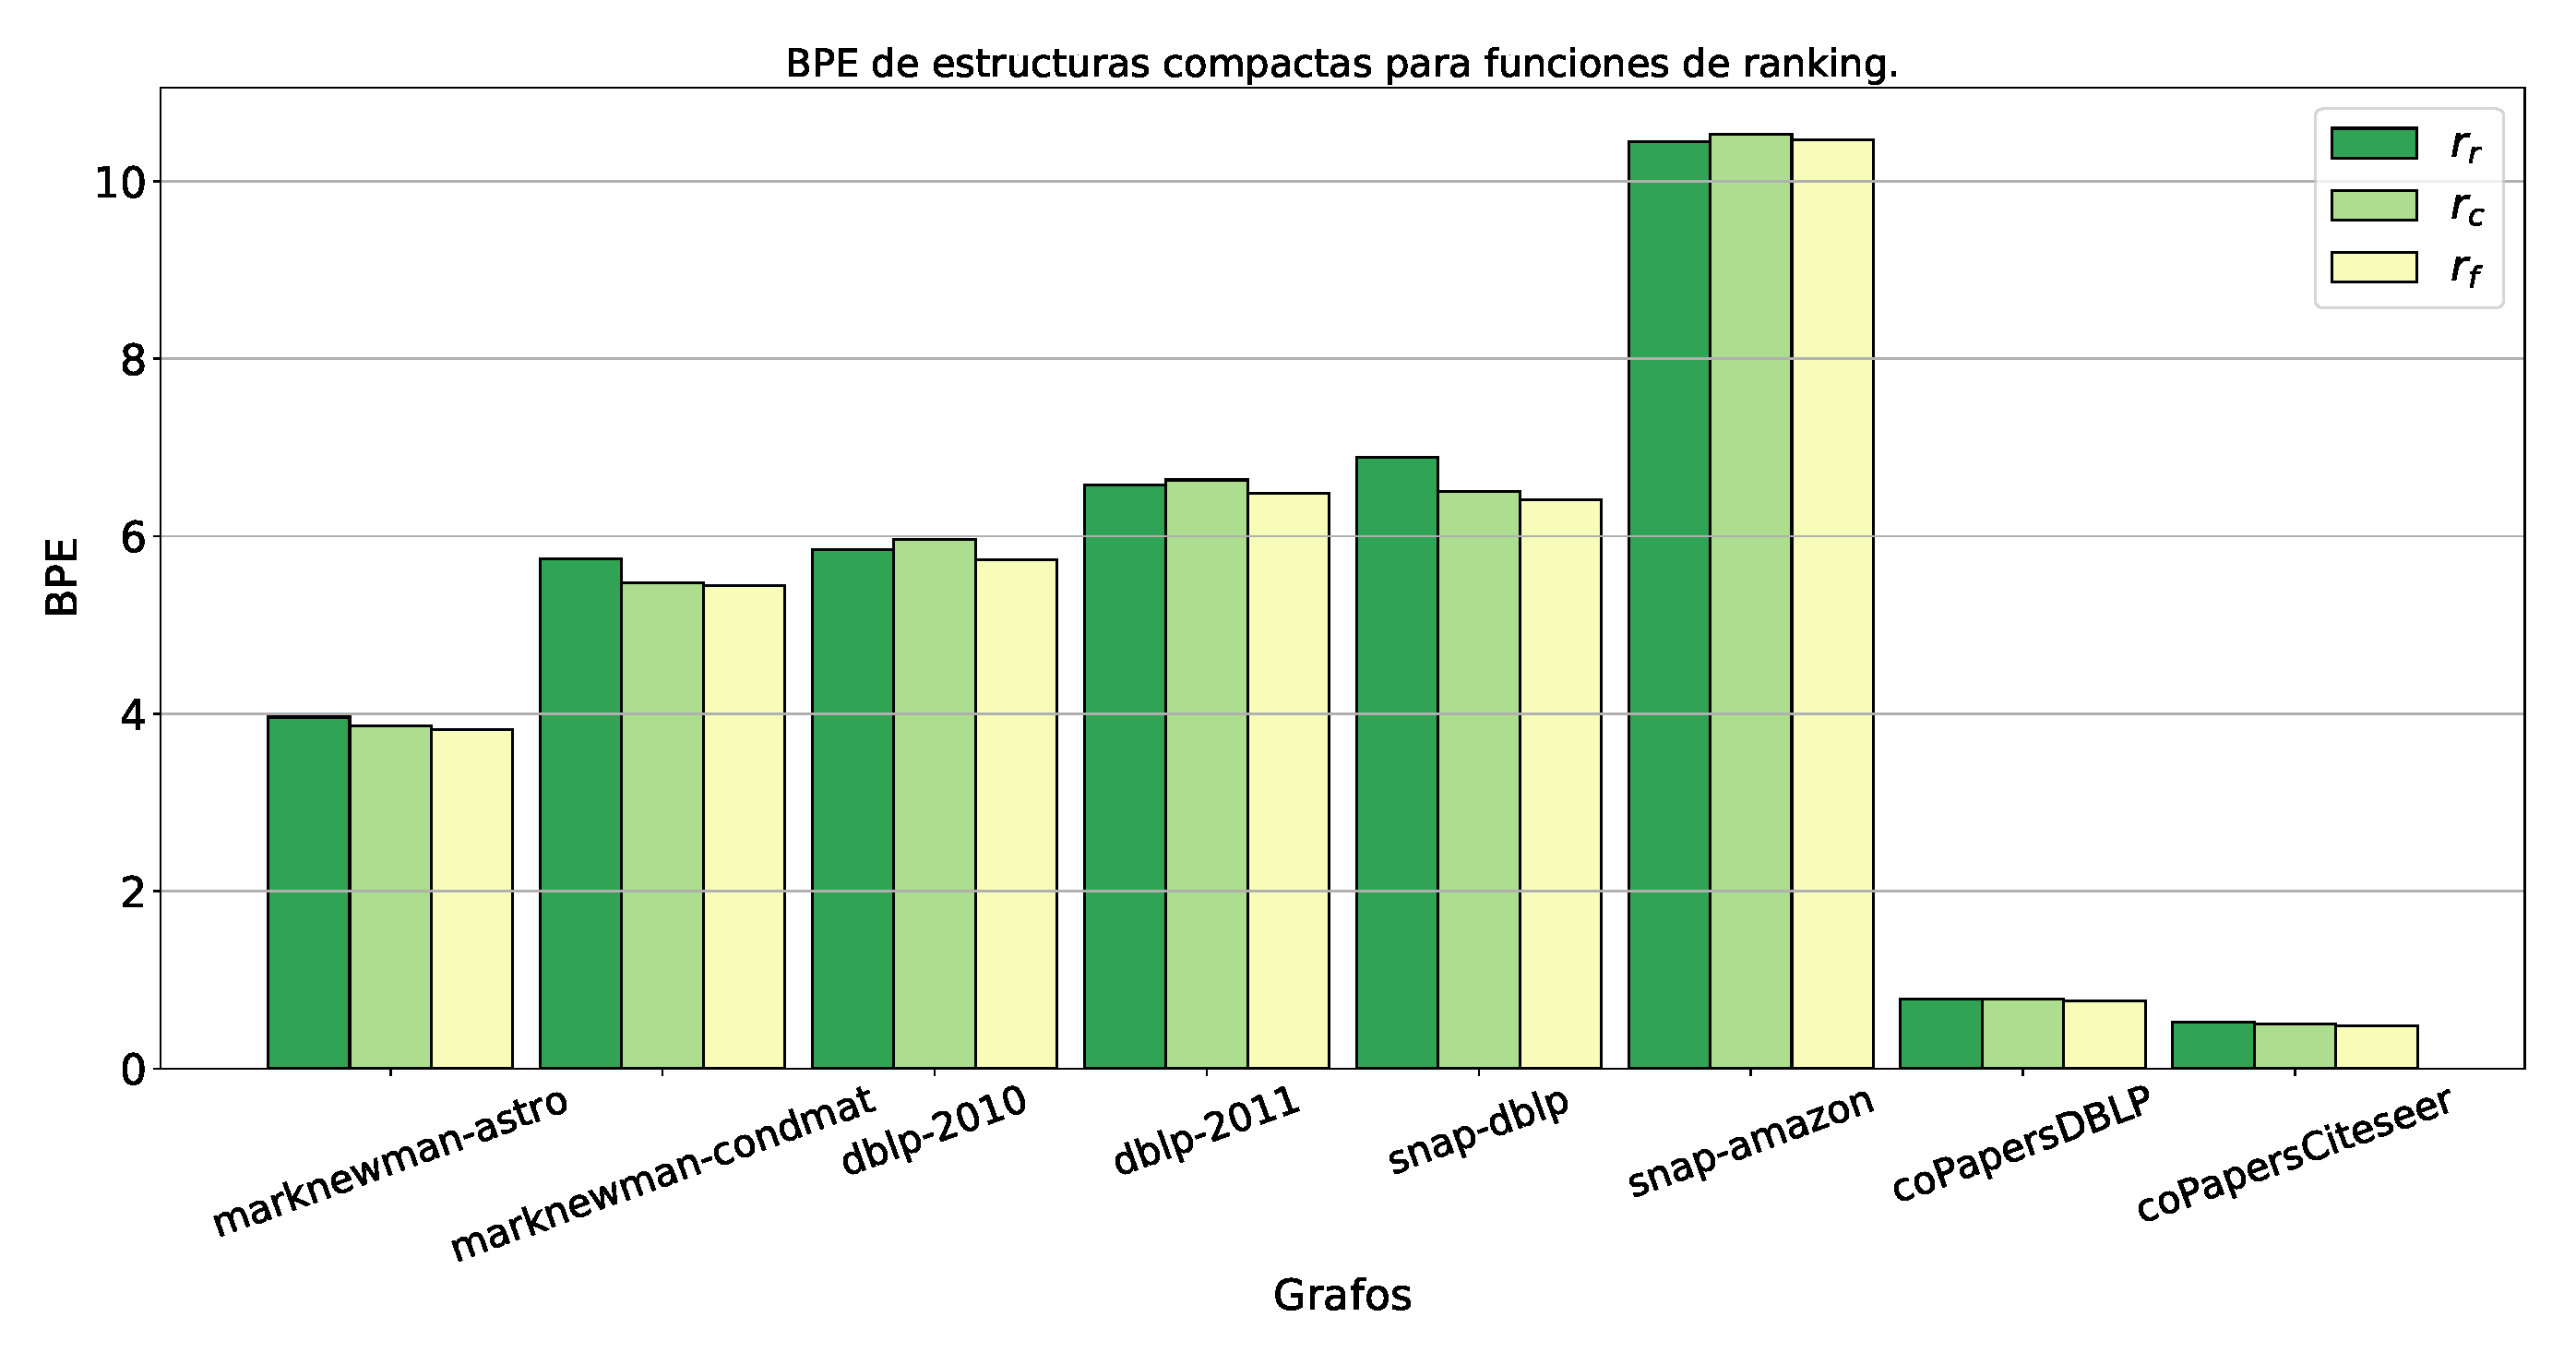
\includegraphics[width=1\linewidth]{../img/bpe3.pdf}
    	
    \caption{BPE de las estructuras compactas para las funciones de ranking.}
\end{figure}

\end{frame}


\begin{frame}
\frametitle{Resultados - Funciones de ranking}

\begin{figure}
    	\centering
    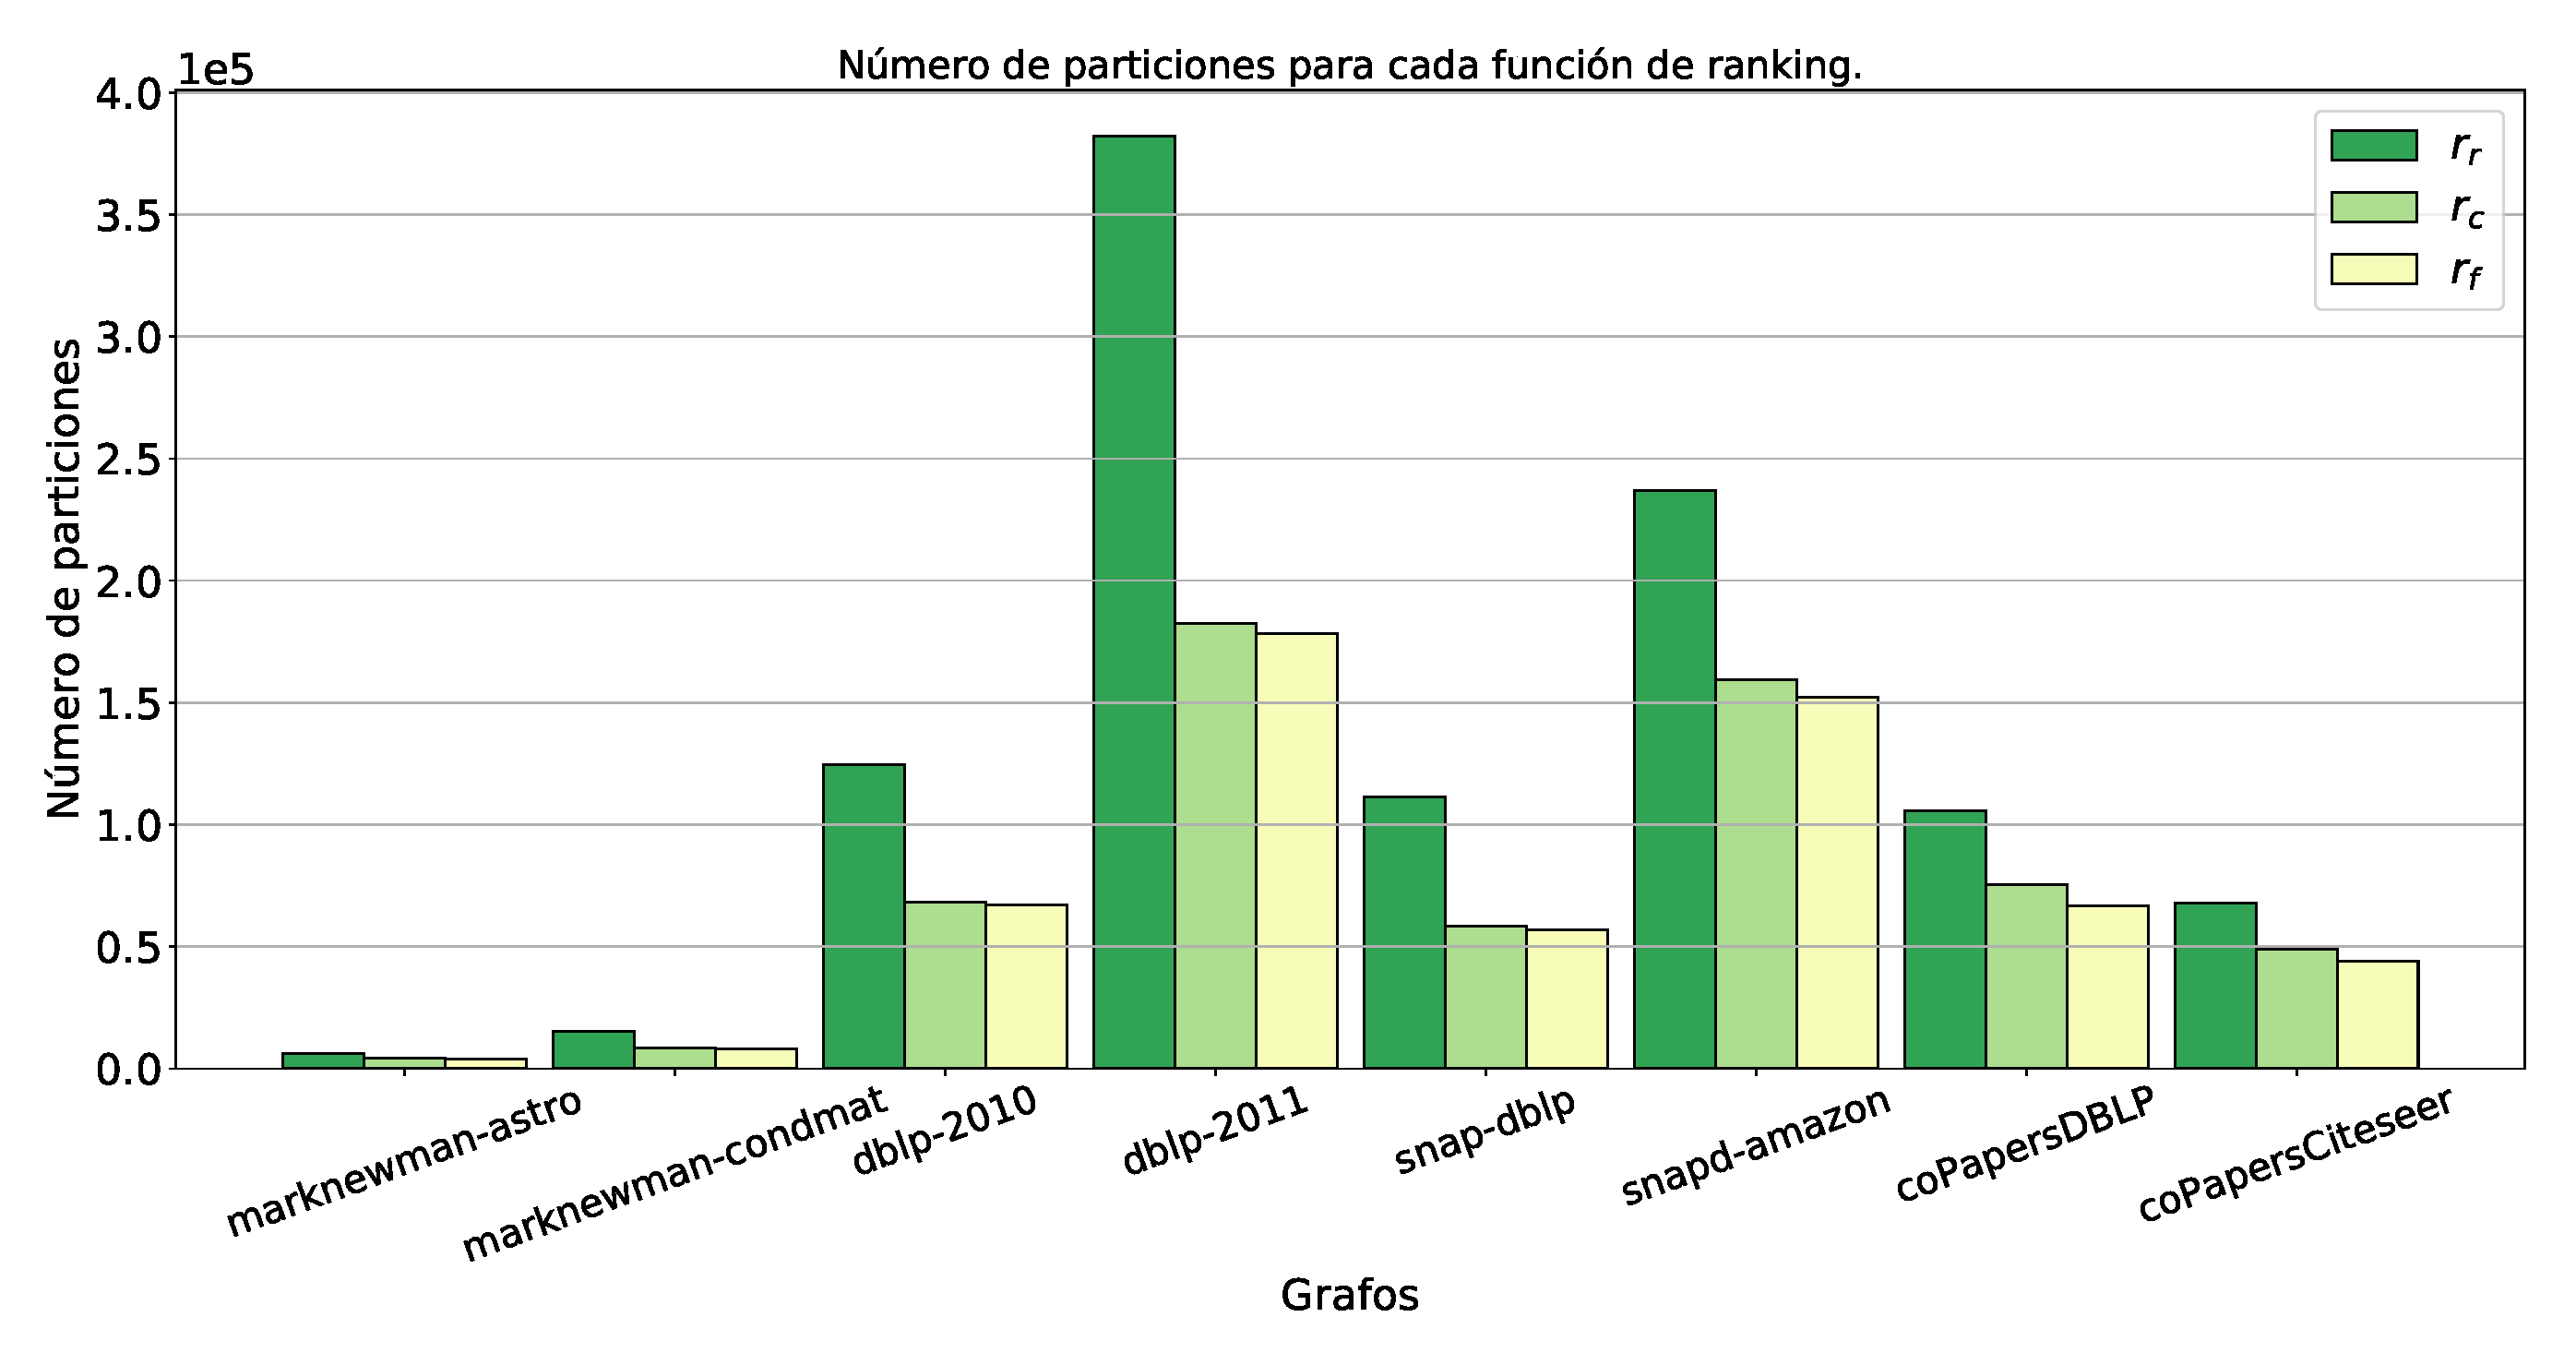
\includegraphics[width=1\linewidth]{../img/Npartitions3.pdf}
    	
    \caption{Número de particiones en las estructuras compactas para las funciones de ranking.}
\end{figure}

\end{frame}

\begin{frame}
\frametitle{Resultados - Funciones de ranking}

\begin{figure}
    	\centering
    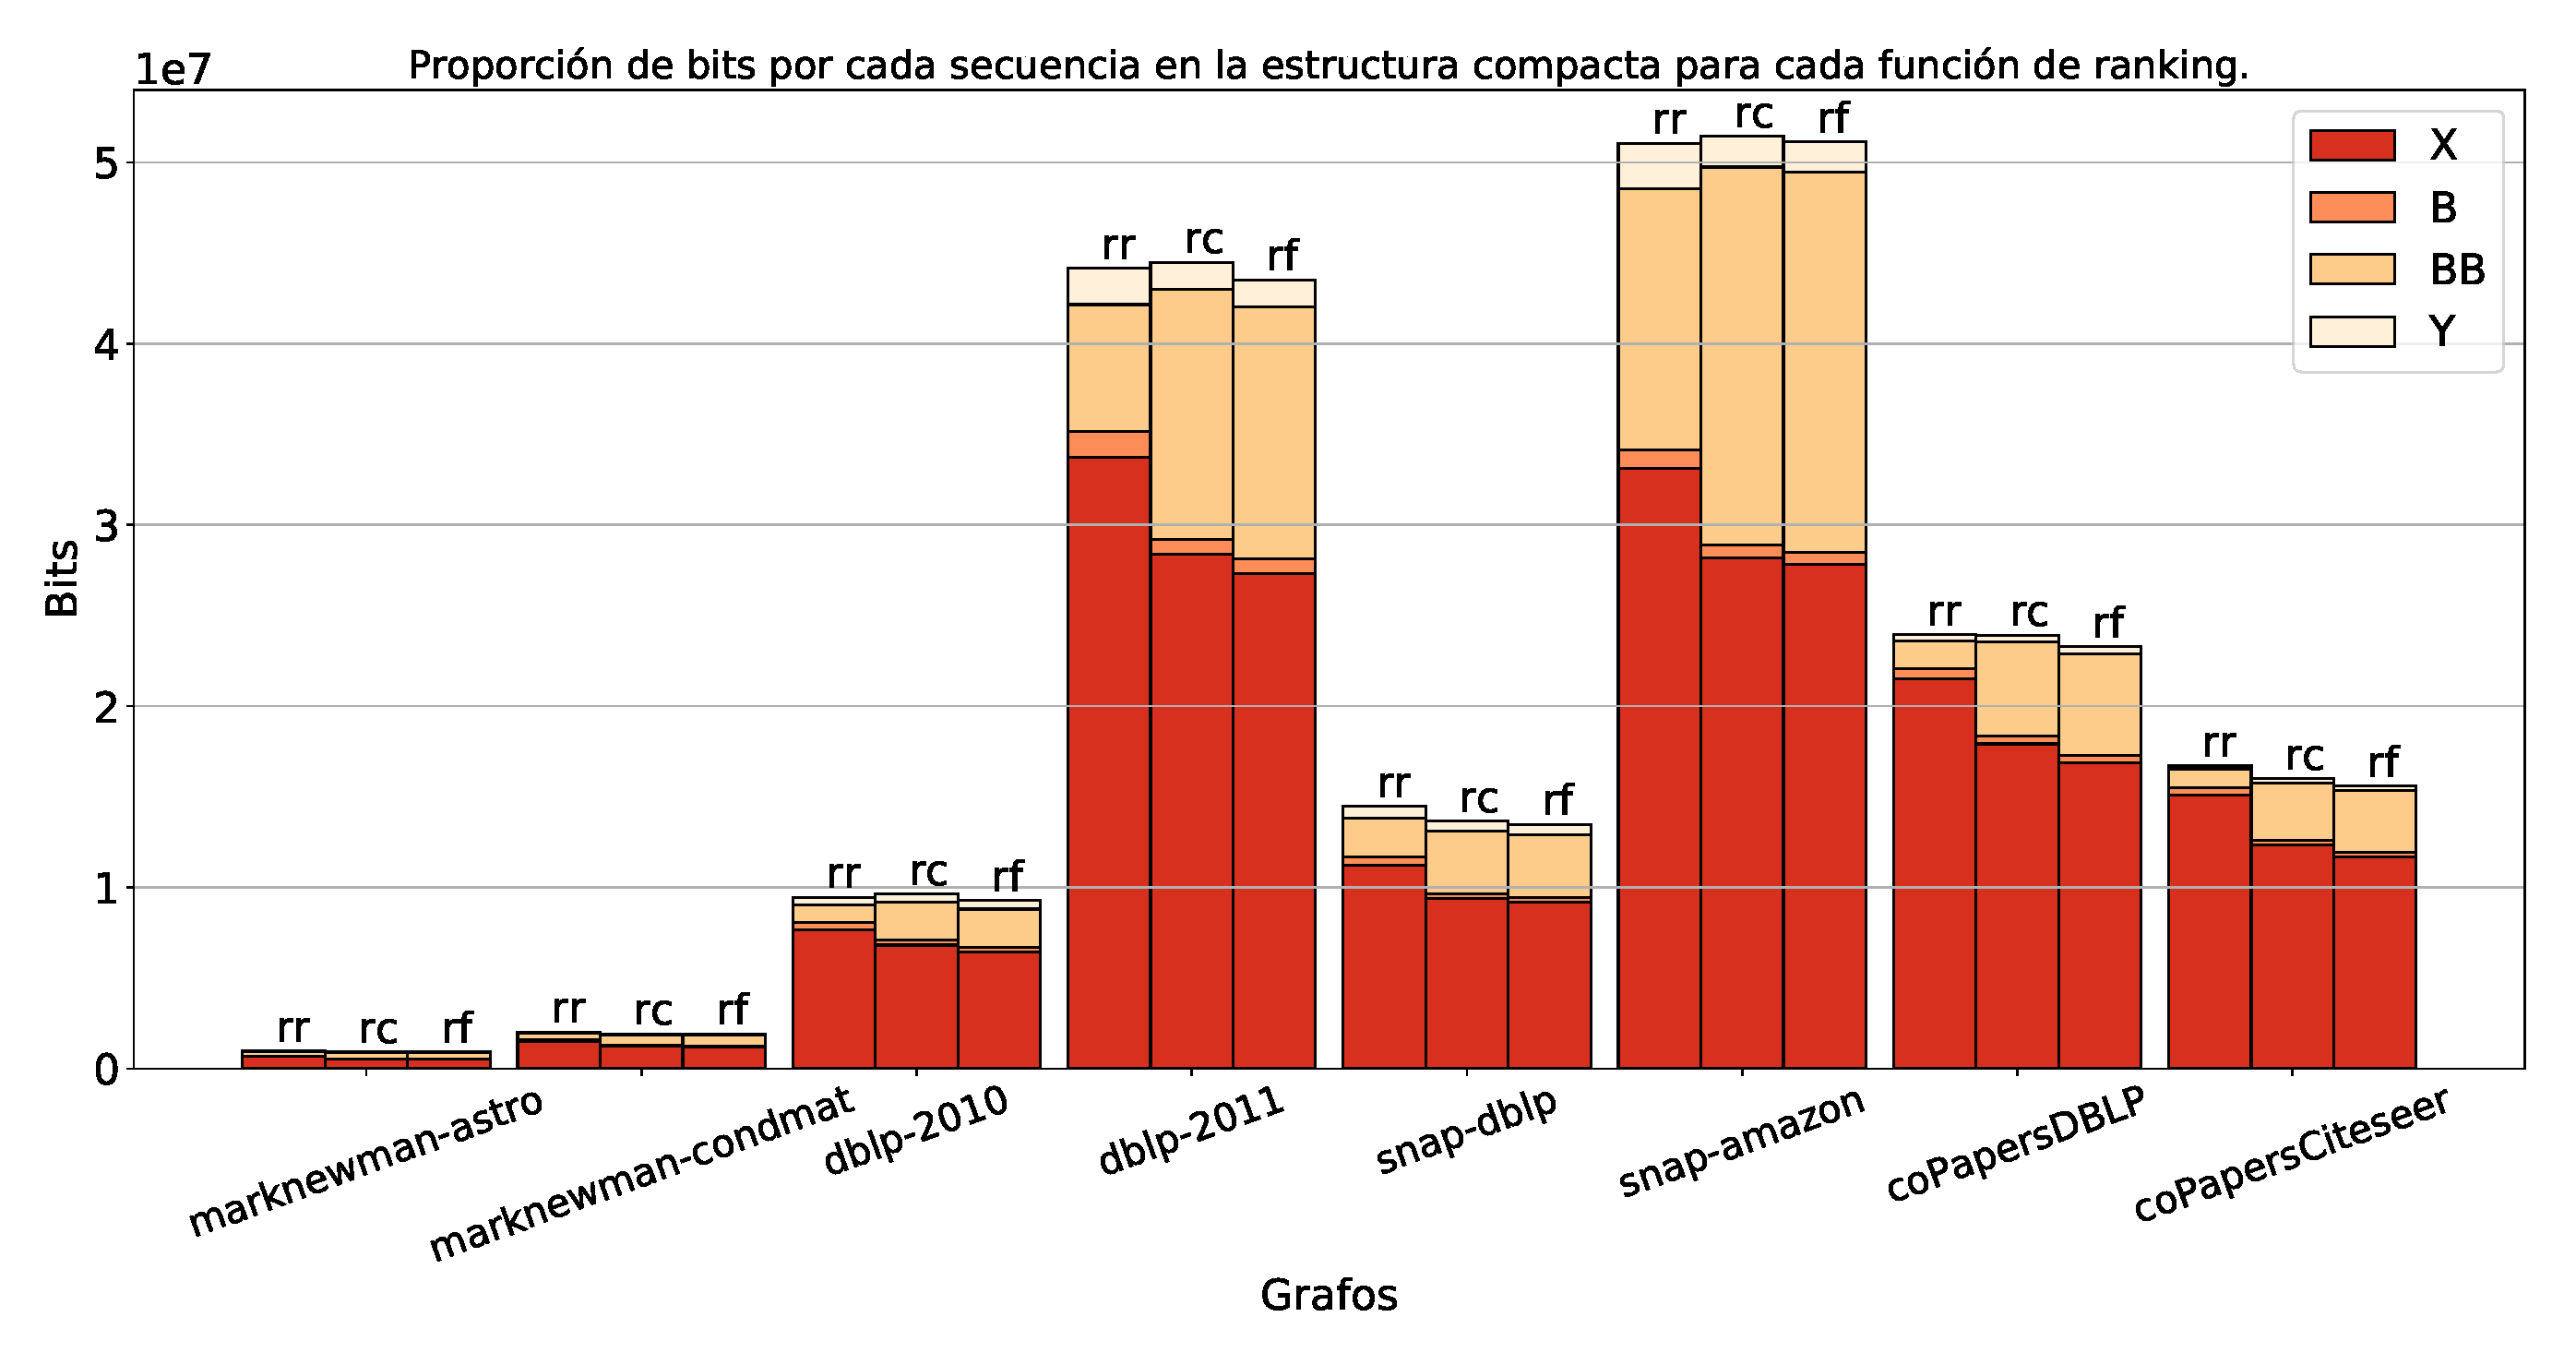
\includegraphics[width=1\linewidth]{../img/bits.pdf}
    	
    \caption{Proporción de bits por cada secuencia en la estructura compacta, para cada función de ranking}
\end{figure}

\end{frame}

\begin{frame}
\frametitle{Resultados - Funciones de ranking}

\begin{figure}
    	\centering
    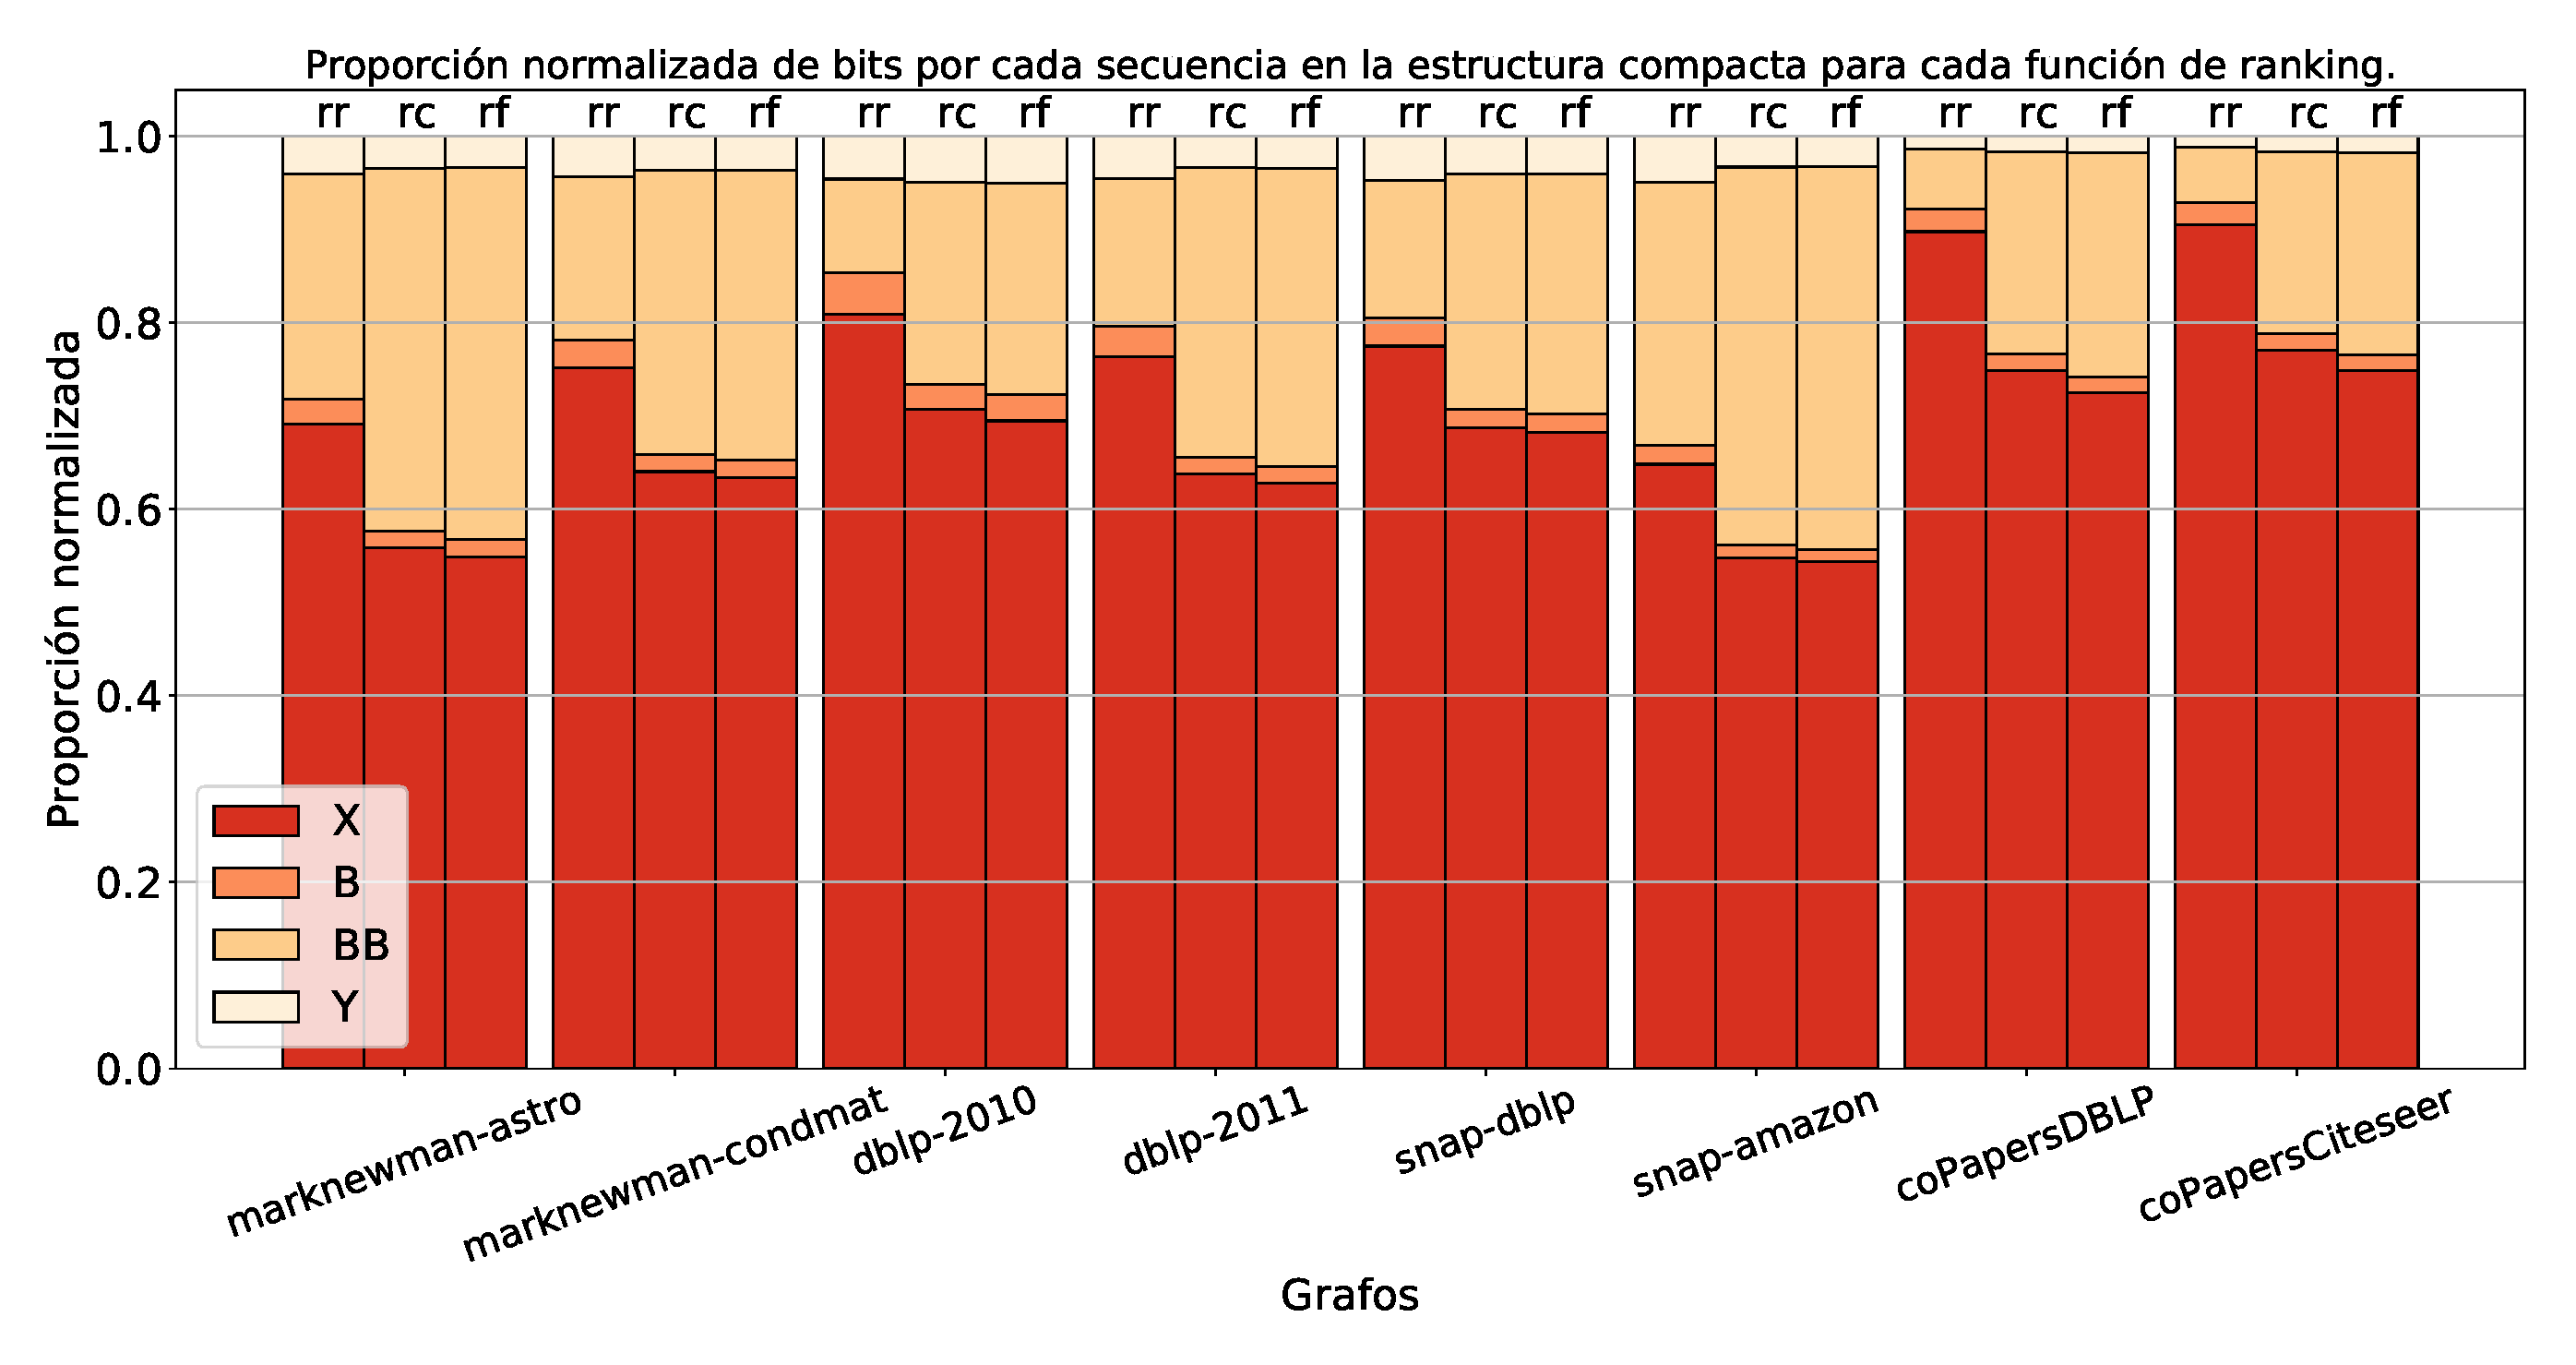
\includegraphics[width=1\linewidth]{../img/bitsNorm.pdf}
    	
    \caption{Proporción normalizada de bits por cada secuencia en la estructura compacta, para cada función de ranking}
\end{figure}

\end{frame}


\begin{frame}
\frametitle{Resultados - Funciones de ranking}

\begin{figure}
    	\centering
    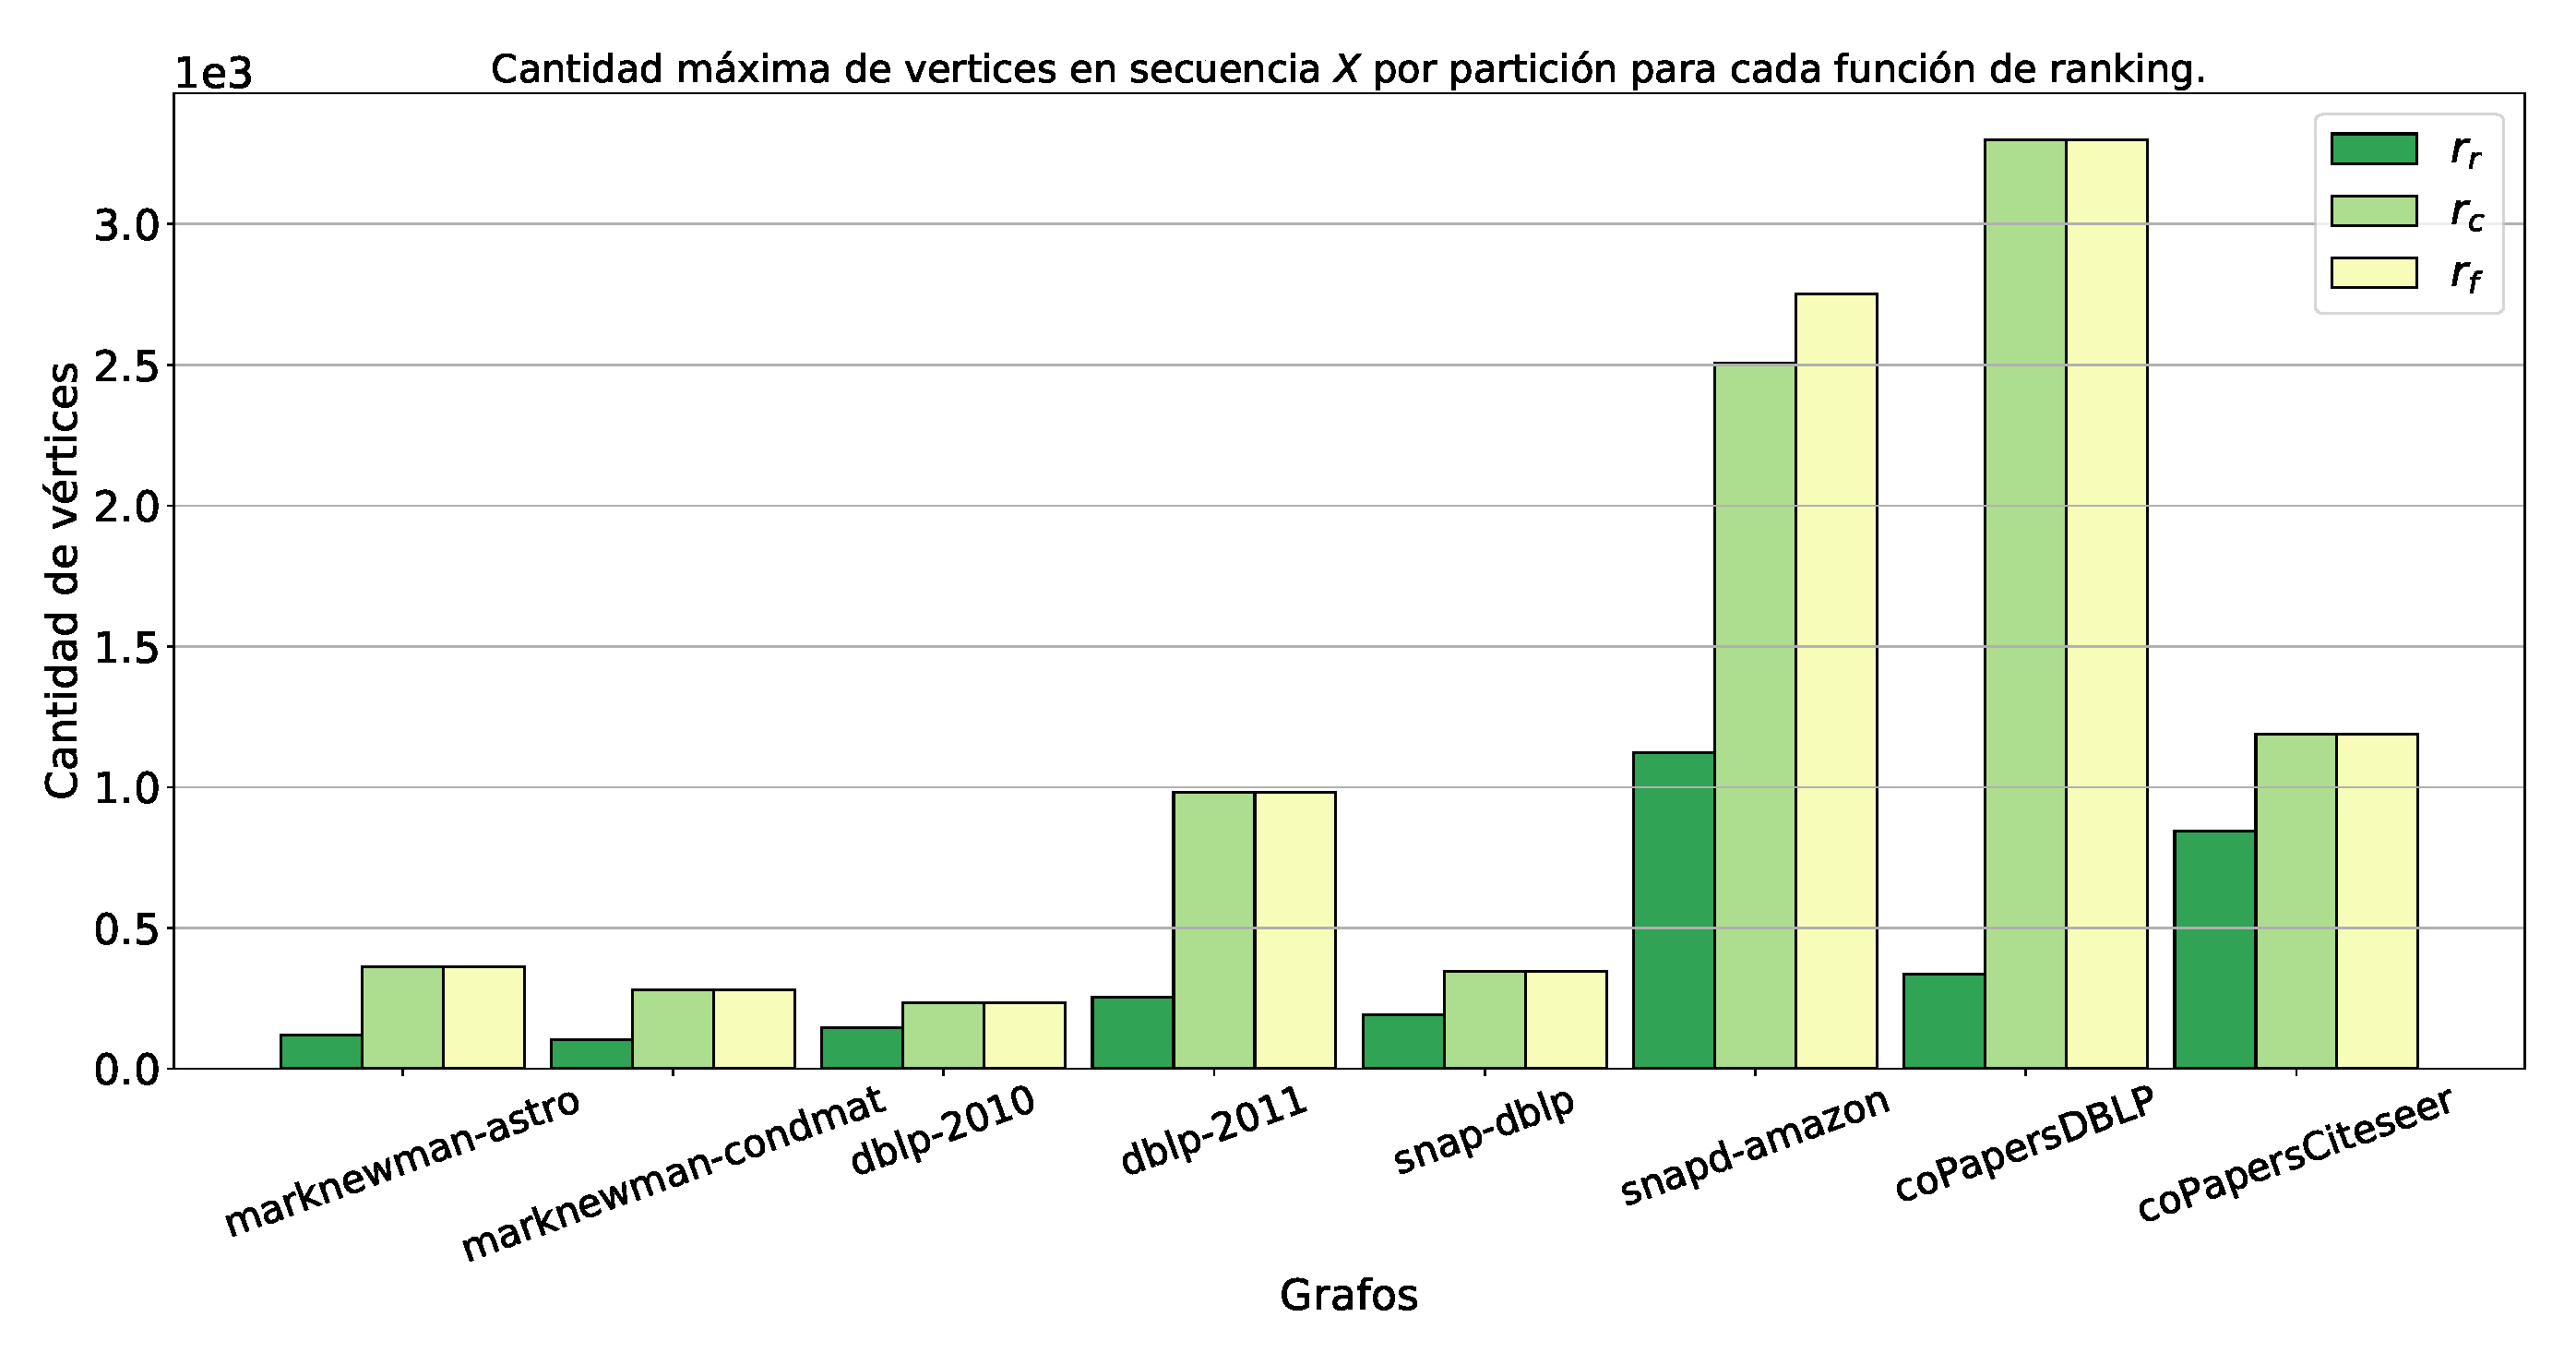
\includegraphics[width=1\linewidth]{../img/maxNodes.pdf}
    	
    \caption{Número máximo de vértices en la secuencia $X$ para las funciones de ranking.}
\end{figure}

\end{frame}

\begin{frame}
\frametitle{Resultados - Funciones de ranking}

\begin{figure}
    	\centering
    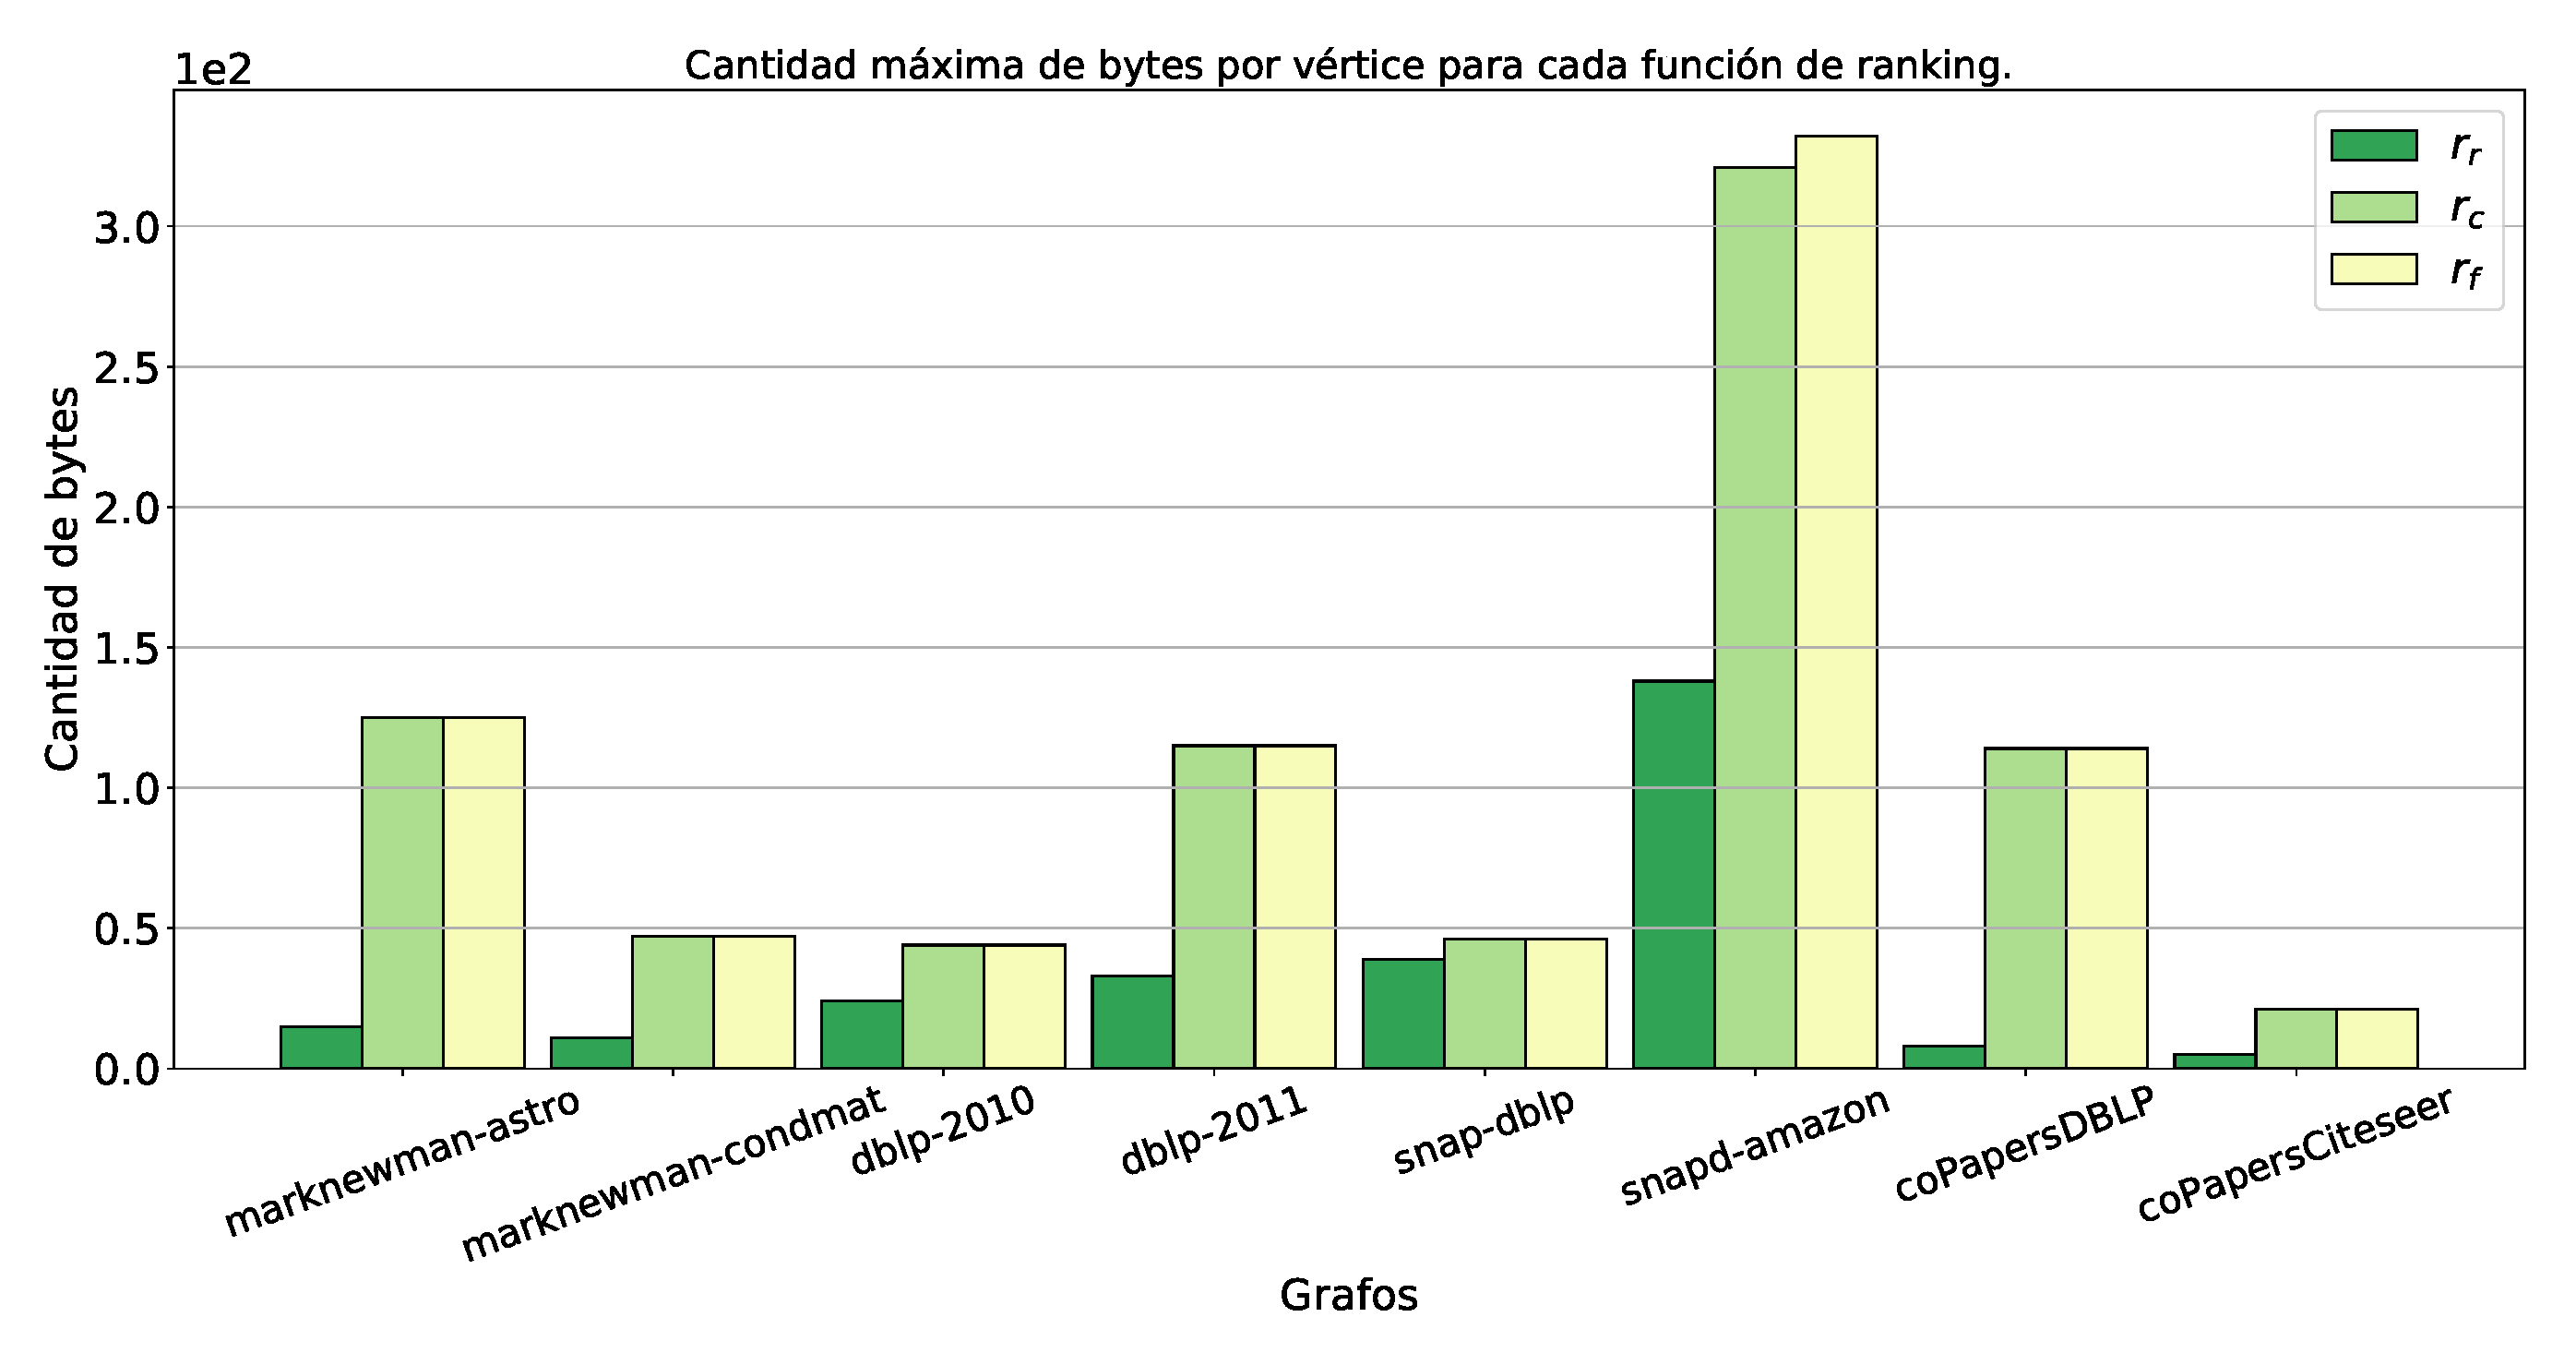
\includegraphics[width=1\linewidth]{../img/maxBytes.pdf}
    	
    \caption{Número máximo de bytes por nodo para las funciones de ranking.}
\end{figure}

\end{frame}



\begin{frame}
\frametitle{Resultados - Funciones de ranking}

\begin{figure}
    \centering
    	\begin{minipage}{1\textwidth}
    		\centering
    		\begin{minipage}{0.45\textwidth}
    			\centering
    			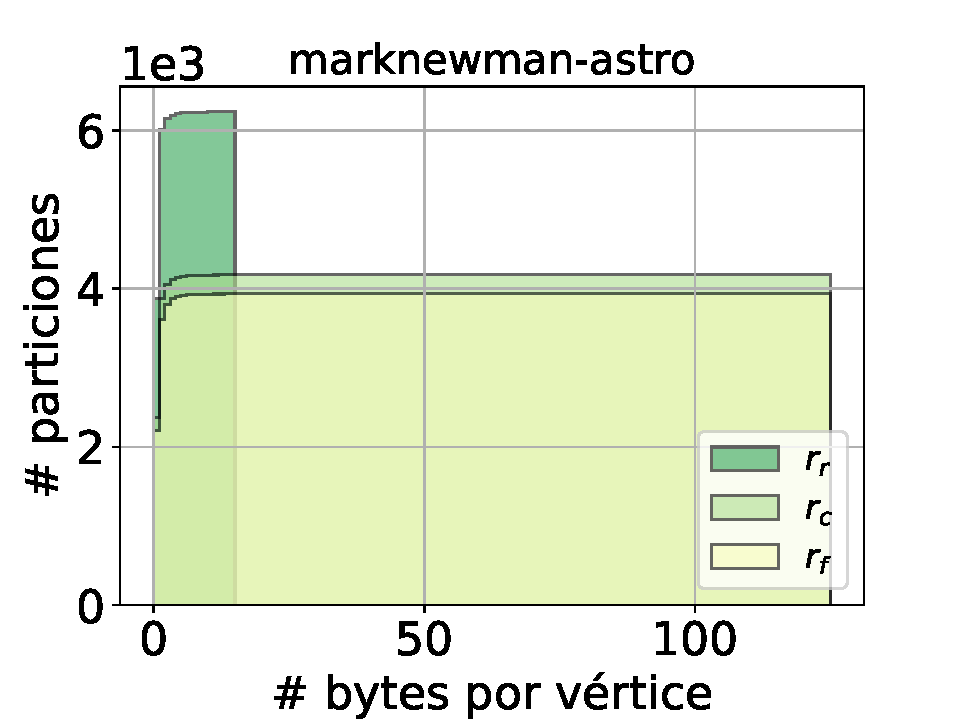
\includegraphics[width=1\linewidth]{../img/cdf/marknewman-astro.pdf}
    		\end{minipage}
    		\begin{minipage}{0.45\textwidth}
    			\centering
    			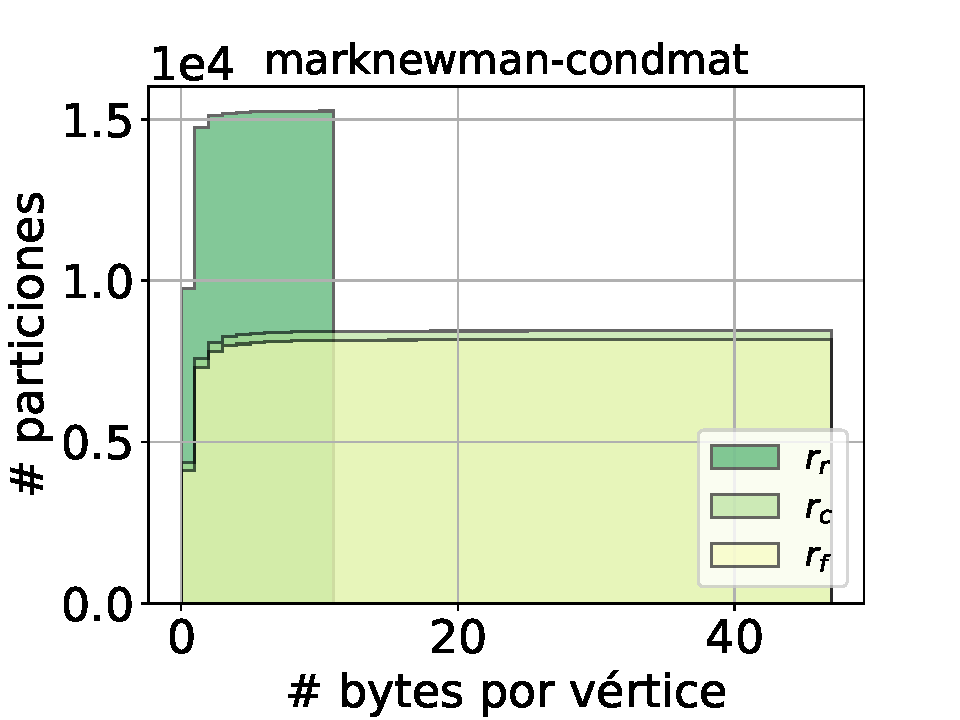
\includegraphics[width=1\linewidth]{../img/cdf/marknewman-condmat.pdf}
    		\end{minipage}  		
    	\end{minipage}
    	
    	\begin{minipage}{1\textwidth}
    		\centering
    		\begin{minipage}{0.45\textwidth}
    			\centering
    			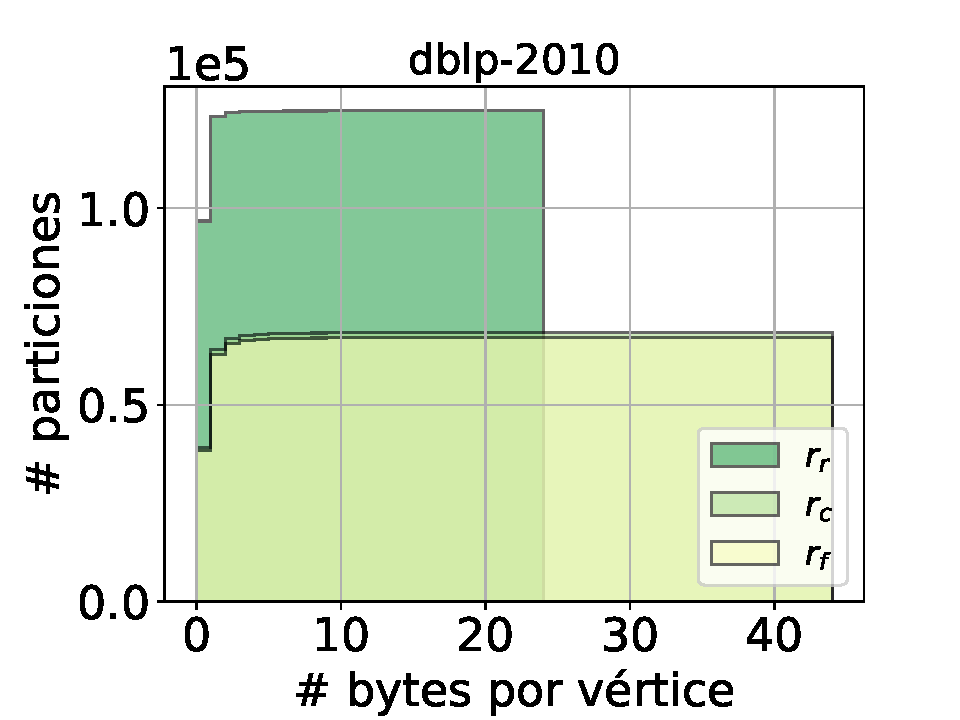
\includegraphics[width=1\linewidth]{../img/cdf/dblp-2010.pdf}
    		\end{minipage}
    		\begin{minipage}{0.45\textwidth}
    			\centering
    			\includegraphics[width=1\linewidth]{../img/cdf/dblp-2011.pdf}
    		\end{minipage}  
    	\end{minipage}	

    \caption{CDF para bytes por vértice en estructuras compactas para cada función de ranking (1).}
\end{figure}


\end{frame}
\begin{frame}%[noframenumbering]
\frametitle{Resultados - Funciones de ranking}

\begin{figure}
    \centering
    	\begin{minipage}{1\textwidth}
    		\centering
    		\begin{minipage}{0.45\textwidth}
    			\centering
    			\includegraphics[width=1\linewidth]{../img/cdf/snap-dblp.pdf}
    		\end{minipage}
    		\begin{minipage}{0.45\textwidth}
    			\centering
    			\includegraphics[width=1\linewidth]{../img/cdf/snap-amazon.pdf}
    		\end{minipage}  		
    	\end{minipage}
    	
    	\begin{minipage}{1\textwidth}
    		\centering
    		\begin{minipage}{0.45\textwidth}
    			\centering
    			\includegraphics[width=1\linewidth]{../img/cdf/coPapersDBLP.pdf}
    		\end{minipage}
    		\begin{minipage}{0.45\textwidth}
    			\centering
    			\includegraphics[width=1\linewidth]{../img/cdf/coPapersCiteseer.pdf}
    		\end{minipage}  
    	\end{minipage}	

    \caption{CDF para bytes por vértice en estructuras compactas para cada función de ranking (2).}
\end{figure}

\end{frame}



\begin{frame}
\frametitle{Resultados - Estructura compacta}

\begin{figure}
	\centering
	
    	\begin{minipage}{1\textwidth}
    		\centering
    		\begin{minipage}{0.8\textwidth}
    			\centering
    			\includegraphics[width=1\linewidth]{../img/sdsl/aleatorioBig/marknewman-astro.pdf}
    		\end{minipage}
    		\begin{minipage}{0.15\textwidth}
    			\centering
    			\includegraphics[scale=.15, clip, trim=70 0 0 0]{../img/sdsl/label.pdf}
    		\end{minipage}	
    	\end{minipage}

	\caption{BPE y Tiempo de acceso aleatorio medio para posibles estructuras compactas, por cada función de ranking, para marknewman-astro.}
\end{figure}

\end{frame}

\begin{frame}
\frametitle{Resultados - Estructura compacta}

\begin{figure}
	\centering
	
    	\begin{minipage}{1\textwidth}
    		\centering
    		\begin{minipage}{0.8\textwidth}
    			\centering
    			\includegraphics[width=1\linewidth]{../img/sdsl/aleatorioBig/marknewman-condmat.pdf}
    		\end{minipage}
    		\begin{minipage}{0.15\textwidth}
    			\centering
    			\includegraphics[scale=.15, clip, trim=70 0 0 0]{../img/sdsl/label.pdf}
    		\end{minipage}	
    	\end{minipage}

	\caption{BPE y Tiempo de acceso aleatorio medio para posibles estructuras compactas, por cada función de ranking, para marknewman-condmat.}
\end{figure}

\end{frame}

\begin{frame}
\frametitle{Resultados - Estructura compacta}

\begin{figure}
	\centering
	
    	\begin{minipage}{1\textwidth}
    		\centering
    		\begin{minipage}{0.8\textwidth}
    			\centering
    			\includegraphics[width=1\linewidth]{../img/sdsl/aleatorioBig/dblp-2010.pdf}
    		\end{minipage}
    		\begin{minipage}{0.15\textwidth}
    			\centering
    			\includegraphics[scale=.15, clip, trim=70 0 0 0]{../img/sdsl/label.pdf}
    		\end{minipage}	
    	\end{minipage}

	\caption{BPE y Tiempo de acceso aleatorio medio para posibles estructuras compactas, por cada función de ranking, para dblp-2010.}
\end{figure}

\end{frame}

\begin{frame}
\frametitle{Resultados - Estructura compacta}

\begin{figure}
	\centering
	
    	\begin{minipage}{1\textwidth}
    		\centering
    		\begin{minipage}{0.8\textwidth}
    			\centering
    			\includegraphics[width=1\linewidth]{../img/sdsl/aleatorioBig/dblp-2011.pdf}
    		\end{minipage}
    		\begin{minipage}{0.15\textwidth}
    			\centering
    			\includegraphics[scale=.15, clip, trim=70 0 0 0]{../img/sdsl/label.pdf}
    		\end{minipage}	
    	\end{minipage}

	\caption{BPE y Tiempo de acceso aleatorio medio para posibles estructuras compactas, por cada función de ranking, para dblp-2011.}
\end{figure}

\end{frame}

\begin{frame}
\frametitle{Resultados - Estructura compacta}

\begin{figure}
	\centering
	
    	\begin{minipage}{1\textwidth}
    		\centering
    		\begin{minipage}{0.8\textwidth}
    			\centering
    			\includegraphics[width=1\linewidth]{../img/sdsl/aleatorioBig/snap-dblp.pdf}
    		\end{minipage}
    		\begin{minipage}{0.15\textwidth}
    			\centering
    			\includegraphics[scale=.15, clip, trim=70 0 0 0]{../img/sdsl/label.pdf}
    		\end{minipage}	
    	\end{minipage}

	\caption{BPE y Tiempo de acceso aleatorio medio para posibles estructuras compactas, por cada función de ranking, para snap-dblp.}
\end{figure}

\end{frame}

\begin{frame}
\frametitle{Resultados - Estructura compacta}

\begin{figure}
	\centering
	
    	\begin{minipage}{1\textwidth}
    		\centering
    		\begin{minipage}{0.8\textwidth}
    			\centering
    			\includegraphics[width=1\linewidth]{../img/sdsl/aleatorioBig/snap-amazon.pdf}
    		\end{minipage}
    		\begin{minipage}{0.15\textwidth}
    			\centering
    			\includegraphics[scale=.15, clip, trim=70 0 0 0]{../img/sdsl/label.pdf}
    		\end{minipage}	
    	\end{minipage}

	\caption{BPE y Tiempo de acceso aleatorio medio para posibles estructuras compactas, por cada función de ranking, para snap-amazon.}
\end{figure}

\end{frame}

\begin{frame}
\frametitle{Resultados - Estructura compacta}

\begin{figure}
	\centering
	
    	\begin{minipage}{1\textwidth}
    		\centering
    		\begin{minipage}{0.8\textwidth}
    			\centering
    			\includegraphics[width=1\linewidth]{../img/sdsl/aleatorioBig/coPapersDBLP.pdf}
    		\end{minipage}
    		\begin{minipage}{0.15\textwidth}
    			\centering
    			\includegraphics[scale=.15, clip, trim=70 0 0 0]{../img/sdsl/label.pdf}
    		\end{minipage}	
    	\end{minipage}

	\caption{BPE y Tiempo de acceso aleatorio medio para posibles estructuras compactas, por cada función de ranking, para coPapersDBLP.}
\end{figure}

\end{frame}

\begin{frame}
\frametitle{Resultados - Estructura compacta}

\begin{figure}
	\centering
	
    	\begin{minipage}{1\textwidth}
    		\centering
    		\begin{minipage}{0.8\textwidth}
    			\centering
    			\includegraphics[width=1\linewidth]{../img/sdsl/aleatorioBig/coPapersCiteseer.pdf}
    		\end{minipage}
    		\begin{minipage}{0.15\textwidth}
    			\centering
    			\includegraphics[scale=.15, clip, trim=70 0 0 0]{../img/sdsl/label.pdf}
    		\end{minipage}	
    	\end{minipage}

	\caption{BPE y Tiempo de acceso aleatorio medio para posibles estructuras compactas, por cada función de ranking, para coPapersCiteseer.}
\end{figure}

\end{frame}


\begin{frame}
\frametitle{Resultados - Estructura compacta}

\begin{figure}
	\centering
	
    	\begin{minipage}{1\textwidth}
    		\centering
    		\begin{minipage}{0.8\textwidth}
    			\centering
    			\includegraphics[width=1\linewidth]{../img/sdsl/secuencialBig/marknewman-astro.pdf}
    		\end{minipage}
    		\begin{minipage}{0.15\textwidth}
    			\centering
    			\includegraphics[scale=.15, clip, trim=70 0 0 0]{../img/sdsl/label.pdf}
    		\end{minipage}	
    	\end{minipage}

	\caption{BPE y Tiempo de acceso secuencial medio para posibles estructuras compactas, por cada función de ranking, para marknewman-astro.}
\end{figure}

\end{frame}

\begin{frame}
\frametitle{Resultados - Estructura compacta}

\begin{figure}
	\centering
	
    	\begin{minipage}{1\textwidth}
    		\centering
    		\begin{minipage}{0.8\textwidth}
    			\centering
    			\includegraphics[width=1\linewidth]{../img/sdsl/secuencialBig/marknewman-condmat.pdf}
    		\end{minipage}
    		\begin{minipage}{0.15\textwidth}
    			\centering
    			\includegraphics[scale=.15, clip, trim=70 0 0 0]{../img/sdsl/label.pdf}
    		\end{minipage}	
    	\end{minipage}

	\caption{BPE y Tiempo de acceso secuencial medio para posibles estructuras compactas, por cada función de ranking, para marknewman-condmat.}
\end{figure}

\end{frame}

\begin{frame}
\frametitle{Resultados - Estructura compacta}

\begin{figure}
	\centering
	
    	\begin{minipage}{1\textwidth}
    		\centering
    		\begin{minipage}{0.8\textwidth}
    			\centering
    			\includegraphics[width=1\linewidth]{../img/sdsl/secuencialBig/dblp-2010.pdf}
    		\end{minipage}
    		\begin{minipage}{0.15\textwidth}
    			\centering
    			\includegraphics[scale=.15, clip, trim=70 0 0 0]{../img/sdsl/label.pdf}
    		\end{minipage}	
    	\end{minipage}

	\caption{BPE y Tiempo de acceso secuencial medio para posibles estructuras compactas, por cada función de ranking, para dblp-2010.}
\end{figure}

\end{frame}

\begin{frame}
\frametitle{Resultados - Estructura compacta}

\begin{figure}
	\centering
	
    	\begin{minipage}{1\textwidth}
    		\centering
    		\begin{minipage}{0.8\textwidth}
    			\centering
    			\includegraphics[width=1\linewidth]{../img/sdsl/secuencialBig/dblp-2011.pdf}
    		\end{minipage}
    		\begin{minipage}{0.15\textwidth}
    			\centering
    			\includegraphics[scale=.15, clip, trim=70 0 0 0]{../img/sdsl/label.pdf}
    		\end{minipage}	
    	\end{minipage}

	\caption{BPE y Tiempo de acceso secuencial medio para posibles estructuras compactas, por cada función de ranking, para dblp-2011.}
\end{figure}

\end{frame}

\begin{frame}
\frametitle{Resultados - Estructura compacta}

\begin{figure}
	\centering
	
    	\begin{minipage}{1\textwidth}
    		\centering
    		\begin{minipage}{0.8\textwidth}
    			\centering
    			\includegraphics[width=1\linewidth]{../img/sdsl/secuencialBig/snap-dblp.pdf}
    		\end{minipage}
    		\begin{minipage}{0.15\textwidth}
    			\centering
    			\includegraphics[scale=.15, clip, trim=70 0 0 0]{../img/sdsl/label.pdf}
    		\end{minipage}	
    	\end{minipage}

	\caption{BPE y Tiempo de acceso secuencial medio para posibles estructuras compactas, por cada función de ranking, para snap-dblp.}
\end{figure}

\end{frame}

\begin{frame}
\frametitle{Resultados - Estructura compacta}

\begin{figure}
	\centering
	
    	\begin{minipage}{1\textwidth}
    		\centering
    		\begin{minipage}{0.8\textwidth}
    			\centering
    			\includegraphics[width=1\linewidth]{../img/sdsl/secuencialBig/snap-amazon.pdf}
    		\end{minipage}
    		\begin{minipage}{0.15\textwidth}
    			\centering
    			\includegraphics[scale=.15, clip, trim=70 0 0 0]{../img/sdsl/label.pdf}
    		\end{minipage}	
    	\end{minipage}

	\caption{BPE y Tiempo de acceso secuencial medio para posibles estructuras compactas, por cada función de ranking, para snap-amazon.}
\end{figure}

\end{frame}

\begin{frame}
\frametitle{Resultados - Estructura compacta}

\begin{figure}
	\centering
	
    	\begin{minipage}{1\textwidth}
    		\centering
    		\begin{minipage}{0.8\textwidth}
    			\centering
    			\includegraphics[width=1\linewidth]{../img/sdsl/secuencialBig/coPapersDBLP.pdf}
    		\end{minipage}
    		\begin{minipage}{0.15\textwidth}
    			\centering
    			\includegraphics[scale=.15, clip, trim=70 0 0 0]{../img/sdsl/label.pdf}
    		\end{minipage}	
    	\end{minipage}

	\caption{BPE y Tiempo de acceso secuencial medio para posibles estructuras compactas, por cada función de ranking, para coPapersDBLP.}
\end{figure}

\end{frame}

\begin{frame}
\frametitle{Resultados - Estructura compacta}

\begin{figure}
	\centering
	
    	\begin{minipage}{1\textwidth}
    		\centering
    		\begin{minipage}{0.8\textwidth}
    			\centering
    			\includegraphics[width=1\linewidth]{../img/sdsl/secuencialBig/coPapersCiteseer.pdf}
    		\end{minipage}
    		\begin{minipage}{0.15\textwidth}
    			\centering
    			\includegraphics[scale=.15, clip, trim=70 0 0 0]{../img/sdsl/label.pdf}
    		\end{minipage}	
    	\end{minipage}

	\caption{BPE y Tiempo de acceso secuencial medio para posibles estructuras compactas, por cada función de ranking, para coPapersCiteseer.}
\end{figure}

\end{frame}






\begin{frame}
\frametitle{Resultados - Comparando con estado del arte}

\begin{figure}
	\centering
	
    	\begin{minipage}{1\textwidth}
    		\centering
    		\begin{minipage}{0.8\textwidth}
    			\centering
    			\includegraphics[width=1\linewidth]{../img/bpeTimes/aleatorio/marknewman-astro.pdf}
    		\end{minipage}
    		\begin{minipage}{0.15\textwidth}
    			\centering
    			\includegraphics[scale=.16, clip, trim=70 200 280 40]{../img/bpeTimes/labelAle.pdf}
    		\end{minipage}	
    	\end{minipage}

	\caption{BPE y tiempo de acceso aleatorio en microsegundos de cada algoritmo, para marknewman-astro.}
\end{figure}

\end{frame}

\begin{frame}
\frametitle{Resultados - Comparando con estado del arte}

\begin{figure}
	\centering
	
    	\begin{minipage}{1\textwidth}
    		\centering
    		\begin{minipage}{0.8\textwidth}
    			\centering
    			\includegraphics[width=1\linewidth]{../img/bpeTimes/aleatorio/marknewman-condmat.pdf}
    		\end{minipage}
    		\begin{minipage}{0.15\textwidth}
    			\centering
    			\includegraphics[scale=.16, clip, trim=70 200 280 40]{../img/bpeTimes/labelAle.pdf}
    		\end{minipage}	
    	\end{minipage}

	\caption{BPE y tiempo de acceso aleatorio en microsegundoss de cada algoritmo, para marknewman-condmat.}
\end{figure}

\end{frame}

\begin{frame}
\frametitle{Resultados - Comparando con estado del arte}

\begin{figure}
	\centering
	
    	\begin{minipage}{1\textwidth}
    		\centering
    		\begin{minipage}{0.8\textwidth}
    			\centering
    			\includegraphics[width=1\linewidth]{../img/bpeTimes/aleatorio/dblp-2010.pdf}
    		\end{minipage}
    		\begin{minipage}{0.15\textwidth}
    			\centering
    			\includegraphics[scale=.16, clip, trim=70 200 280 40]{../img/bpeTimes/labelAle.pdf}
    		\end{minipage}	
    	\end{minipage}

	\caption{BPE y tiempo de acceso aleatorio en microsegundos de cada algoritmo, para dblp-2010.}
\end{figure}

\end{frame}

\begin{frame}
\frametitle{Resultados - Comparando con estado del arte}

\begin{figure}
	\centering
	
    	\begin{minipage}{1\textwidth}
    		\centering
    		\begin{minipage}{0.8\textwidth}
    			\centering
    			\includegraphics[width=1\linewidth]{../img/bpeTimes/aleatorio/dblp-2011.pdf}
    		\end{minipage}
    		\begin{minipage}{0.15\textwidth}
    			\centering
    			\includegraphics[scale=.16, clip, trim=70 200 280 40]{../img/bpeTimes/labelAle.pdf}
    		\end{minipage}	
    	\end{minipage}

	\caption{BPE y tiempo de acceso aleatorio en microsegundos de cada algoritmo, para dblp-2011.}
\end{figure}

\end{frame}

\begin{frame}
\frametitle{Resultados - Comparando con estado del arte}

\begin{figure}
	\centering
	
    	\begin{minipage}{1\textwidth}
    		\centering
    		\begin{minipage}{0.8\textwidth}
    			\centering
    			\includegraphics[width=1\linewidth]{../img/bpeTimes/aleatorio/snap-dblp.pdf}
    		\end{minipage}
    		\begin{minipage}{0.15\textwidth}
    			\centering
    			\includegraphics[scale=.16, clip, trim=70 200 280 40]{../img/bpeTimes/labelAle.pdf}
    		\end{minipage}	
    	\end{minipage}

	\caption{BPE y tiempo de acceso aleatorio en microsegundos de cada algoritmo, para snap-dblp.}
\end{figure}

\end{frame}

\begin{frame}
\frametitle{Resultados - Comparando con estado del arte}

\begin{figure}
	\centering
	
    	\begin{minipage}{1\textwidth}
    		\centering
    		\begin{minipage}{0.8\textwidth}
    			\centering
    			\includegraphics[width=1\linewidth]{../img/bpeTimes/aleatorio/snap-amazon.pdf}
    		\end{minipage}
    		\begin{minipage}{0.15\textwidth}
    			\centering
    			\includegraphics[scale=.16, clip, trim=70 200 280 40]{../img/bpeTimes/labelAle.pdf}
    		\end{minipage}	
    	\end{minipage}

	\caption{BPE y tiempo de acceso aleatorio en microsegundos de cada algoritmo, para snap-amazon.}
\end{figure}

\end{frame}

\begin{frame}
\frametitle{Resultados - Comparando con estado del arte}

\begin{figure}
	\centering
	
    	\begin{minipage}{1\textwidth}
    		\centering
    		\begin{minipage}{0.8\textwidth}
    			\centering
    			\includegraphics[width=1\linewidth]{../img/bpeTimes/aleatorio/coPapersDBLP.pdf}
    		\end{minipage}
    		\begin{minipage}{0.15\textwidth}
    			\centering
    			\includegraphics[scale=.16, clip, trim=70 200 280 40]{../img/bpeTimes/labelAle.pdf}
    		\end{minipage}	
    	\end{minipage}

	\caption{BPE y tiempo de acceso aleatorio en microsegundos de cada algoritmo, para coPapersDBLP.}
\end{figure}

\end{frame}

\begin{frame}
\frametitle{Resultados - Comparando con estado del arte}

\begin{figure}
	\centering
	
    	\begin{minipage}{1\textwidth}
    		\centering
    		\begin{minipage}{0.8\textwidth}
    			\centering
    			\includegraphics[width=1\linewidth]{../img/bpeTimes/aleatorio/coPapersCiteseer.pdf}
    		\end{minipage}
    		\begin{minipage}{0.15\textwidth}
    			\centering
    			\includegraphics[scale=.16, clip, trim=70 200 280 40]{../img/bpeTimes/labelAle.pdf}
    		\end{minipage}	
    	\end{minipage}

	\caption{BPE y tiempo de acceso aleatorio en microsegundos de cada algoritmo, para coPapersCiteseer.}
\end{figure}

\end{frame}





\begin{frame}
\frametitle{Resultados - Comparando con estado del arte}

\begin{figure}
	\centering
	
    	\begin{minipage}{1\textwidth}
    		\centering
    		\begin{minipage}{0.8\textwidth}
    			\centering
    			\includegraphics[width=1\linewidth]{../img/bpeTimes/secuencial/marknewman-astro.pdf}
    		\end{minipage}
    		\begin{minipage}{0.15\textwidth}
    			\centering
    			\includegraphics[scale=.16, clip, trim=70 200 280 40]{../img/bpeTimes/labelSec.pdf}
    		\end{minipage}	
    	\end{minipage}

	\caption{BPE y tiempo de reconstrucción secuencial en segundos de cada algoritmo, para marknewman-astro.}
\end{figure}

\end{frame}

\begin{frame}
\frametitle{Resultados - Comparando con estado del arte}

\begin{figure}
	\centering
	
    	\begin{minipage}{1\textwidth}
    		\centering
    		\begin{minipage}{0.8\textwidth}
    			\centering
    			\includegraphics[width=1\linewidth]{../img/bpeTimes/secuencial/marknewman-condmat.pdf}
    		\end{minipage}
    		\begin{minipage}{0.15\textwidth}
    			\centering
    			\includegraphics[scale=.16, clip, trim=70 200 280 40]{../img/bpeTimes/labelSec.pdf}
    		\end{minipage}	
    	\end{minipage}

	\caption{BPE y tiempo de reconstrucción secuencial en segundos de cada algoritmo, para marknewman-condmat.}
\end{figure}

\end{frame}

\begin{frame}
\frametitle{Resultados - Comparando con estado del arte}

\begin{figure}
	\centering
	
    	\begin{minipage}{1\textwidth}
    		\centering
    		\begin{minipage}{0.8\textwidth}
    			\centering
    			\includegraphics[width=1\linewidth]{../img/bpeTimes/secuencial/dblp-2010.pdf}
    		\end{minipage}
    		\begin{minipage}{0.15\textwidth}
    			\centering
    			\includegraphics[scale=.16, clip, trim=70 200 280 40]{../img/bpeTimes/labelSec.pdf}
    		\end{minipage}	
    	\end{minipage}

	\caption{BPE y tiempo de reconstrucción secuencial en segundos de cada algoritmo, para dblp-2010.}
\end{figure}

\end{frame}

\begin{frame}
\frametitle{Resultados - Comparando con estado del arte}

\begin{figure}
	\centering
	
    	\begin{minipage}{1\textwidth}
    		\centering
    		\begin{minipage}{0.8\textwidth}
    			\centering
    			\includegraphics[width=1\linewidth]{../img/bpeTimes/secuencial/dblp-2011.pdf}
    		\end{minipage}
    		\begin{minipage}{0.15\textwidth}
    			\centering
    			\includegraphics[scale=.16, clip, trim=70 200 280 40]{../img/bpeTimes/labelSec.pdf}
    		\end{minipage}	
    	\end{minipage}

	\caption{BPE y tiempo de reconstrucción secuencial en segundos de cada algoritmo, para dblp-2011.}
\end{figure}

\end{frame}

\begin{frame}
\frametitle{Resultados - Comparando con estado del arte}

\begin{figure}
	\centering
	
    	\begin{minipage}{1\textwidth}
    		\centering
    		\begin{minipage}{0.8\textwidth}
    			\centering
    			\includegraphics[width=1\linewidth]{../img/bpeTimes/secuencial/snap-dblp.pdf}
    		\end{minipage}
    		\begin{minipage}{0.15\textwidth}
    			\centering
    			\includegraphics[scale=.16, clip, trim=70 200 280 40]{../img/bpeTimes/labelSec.pdf}
    		\end{minipage}	
    	\end{minipage}

	\caption{BPE y tiempo de reconstrucción secuencial en segundos de cada algoritmo, para snap-dblp.}
\end{figure}

\end{frame}

\begin{frame}
\frametitle{Resultados - Comparando con estado del arte}

\begin{figure}
	\centering
	
    	\begin{minipage}{1\textwidth}
    		\centering
    		\begin{minipage}{0.8\textwidth}
    			\centering
    			\includegraphics[width=1\linewidth]{../img/bpeTimes/secuencial/snap-amazon.pdf}
    		\end{minipage}
    		\begin{minipage}{0.15\textwidth}
    			\centering
    			\includegraphics[scale=.16, clip, trim=70 200 280 40]{../img/bpeTimes/labelSec.pdf}
    		\end{minipage}	
    	\end{minipage}

	\caption{BPE y tiempo de reconstrucción secuencial en segundos de cada algoritmo, para snap-amazon.}
\end{figure}

\end{frame}

\begin{frame}
\frametitle{Resultados - Comparando con estado del arte}

\begin{figure}
	\centering
	
    	\begin{minipage}{1\textwidth}
    		\centering
    		\begin{minipage}{0.8\textwidth}
    			\centering
    			\includegraphics[width=1\linewidth]{../img/bpeTimes/secuencial/coPapersDBLP.pdf}
    		\end{minipage}
    		\begin{minipage}{0.15\textwidth}
    			\centering
    			\includegraphics[scale=.16, clip, trim=70 200 280 40]{../img/bpeTimes/labelSec.pdf}
    		\end{minipage}	
    	\end{minipage}

	\caption{BPE y tiempo de reconstrucción secuencial en segundos de cada algoritmo, para coPapersDBLP.}
\end{figure}

\end{frame}

\begin{frame}
\frametitle{Resultados - Comparando con estado del arte}

\begin{figure}
	\centering
	
    	\begin{minipage}{1\textwidth}
    		\centering
    		\begin{minipage}{0.8\textwidth}
    			\centering
    			\includegraphics[width=1\linewidth]{../img/bpeTimes/secuencial/coPapersCiteseer.pdf}
    		\end{minipage}
    		\begin{minipage}{0.15\textwidth}
    			\centering
    			\includegraphics[scale=.16, clip, trim=70 200 280 40]{../img/bpeTimes/labelSec.pdf}
    		\end{minipage}	
    	\end{minipage}

	\caption{BPE y tiempo de reconstrucción secuencial en segundos de cada algoritmo, para coPapersCiteseer.}
\end{figure}

\end{frame}



%%%%%%%%%%%%%%%%%%%%%%%%%%%%%%%%%%%%%%%%%%%%%%%%%%%%%%%%%%%%%%%%%%%%%%%%%%%%%%%%
%
% Paso 17: Conclusiones
%
% 
%%%%%%%%%%%%%%%%%%%%%%%%%%%%%%%%%%%%%%%%%%%%%%%%%%%%%%%%%%%%%%%%%%%%%%%%%%%%%%%%


\chapter{CONCLUSIONES}\label{chap:conclusion}
\vskip 3.0ex

En este trabajo se desarrolla un método de compresión de grafos no dirigidos y poco densos, basado en clustering de cliques maximales, usando estructuras compactas. Se logra llegar a una representación comprimida que permite responder consultas básicas como listado de vecinos de un nodo y reconstrucción del grafo, y otras consultas novedosas como obtener el listado de cliques maximales o saber si dos nodos son vecinos, todo sin tener que descomprimir el grafo.

El nivel de compresión, medido en BPE, es bastante competitivo al estado del arte. La nueva versión de k2tree con BFS en general es mejor, pero en algunos grafos, sobre todo los más grandes y con coeficiente de clustering alto, el método propuesto logra resultados similares. Comparado con los otros algoritmos, el resultado en compresión es bastante mejor, sobre todo comparado con WebGraph. Los mejores BPE se logran con los grafos \texttt{coPapersDBLP} (0,76) y \texttt{coPapersCiteseer} (0,48), los cuales presentan los índices de clusterización más altos, muy pocos cliques comparado con la cantidad de nodos, y la mayoría de dichos cliques con al menos 100 nodos.

Para el tiempo de acceso aleatorio, medido como los segundos por arco que toma recuperar vecinos para un millón de nodos, en varios casos se logran mejores resultados que ambos algoritmos de k2tree, pero no logra superar a AD ni menos a WebGraph, que mantiene total predominancia en este ámbito. Analizando junto al resultado en BPE, se puede apreciar que la propuesta se mantiene competitiva, siempre en la zona media de la comparación. El mejor balance lo logran los grafos \texttt{marknewman-condmat}, \texttt{dblp-2010}, \texttt{dblp-2011}, y \texttt{snap-dblp}, todos los cuales poseen una cantidad similar entre vértices y cliques maximales. Además, comparado con k2tree, 3 de estos grafos ocupan más espacio pero tienen mejor tiempo de acceso, y otros casos como \texttt{coPapersDBLP} ocupa menos espacio pero empeora el tiempo. Mención especial \texttt{snap-amazon}, que contiene más del doble de cliques que vértices, y también logra un buen balance.

Para el tiempo de reconstrucción secuencial del grafo, la estructura propuesta presenta su menor desempeño. En todos los casos, alguna versión de k2tree logra una respuesta más rápida, del orden de 4 veces mejor. Se destaca que para los grafos \texttt{marknewman-astro}, \texttt{marknewman-condmat} y \texttt{dblp-2010}, el método logra mejor tiempo que WebGraph.

En cuanto al tiempo de recuperar el listado de cliques maximales, la propuesta es mucho mas rápida que el algoritmo \textbf{Quick Cliques}\footnote{\url{https://github.com/darrenstrash/quick-cliques}} y si bien es cierto que para generar la estructura se debe generar dicho listado previamente, una vez comprimido el grafo se puede volver a obtener en un tiempo menor. Especial atención a los grafos \texttt{coPapersDBLP} y \texttt{coPapersCiteseer}, que son los grafos con menor BPE, y recuperan el listado de cliques más de 10 veces más rápido. Además esta operación no es fácil de realizar usando las otras técnicas de compresión comparadas.

Esta propuesta además posee la consulta que permite saber si dos vértices son vecinos, sin tener que generar los listados de adyacencia de ninguno de los dos, directamente de la estructura, y en un tiempo  $O((M_{1} + M_{2}) \cdot bpu_{p})$ cuando hay bytes en las particiones, o $O(M_{1} + M_{2})$ si no los hay, siendo $M_{1}$ la cantidad de particiones que contienen al vértice 1, y $M_{2}$ al vértice 2. 

Con esto en consideración, una buena aplicación para el método propuesto son máquinas donde el espacio para guardar el grafo sea limitado, como dispositivos móviles con poca RAM y espacio en disco, donde se pueden almacenar los grafos gracias al buen nivel de compresión, y además permite responder consultas sin ocupar espacio en la descompresión, pagando un tiempo algo mayor.

Como trabajo futuro, se puede explorar cómo mejorar los tiempos de acceso de esta estructura, por ejemplo investigar nuevas funciones de ranking en la heurística de clusterización. Otra opción es explotar el potencial de paralelismo que posee la estructura compacta, ya que cada partición se puede acceder de manera simultánea, y cada comparación de bytes dentro de las particiones se puede optimizar usando instrucciones paralelas como SIMD\footnote{SIMD: Single Instruction, Multiple Data. Una Instrucción, múltiples datos.}.




%%%%%%%%%%%%%%%%%%%%%%%%%%%%%%%%%%%%%%%%%%%%%%%%%%%%%%%%%%%%%%%%%%%%%%%%%%%%%%%%
%
% Paso 18: Bibliografía
%
% Para compilar seguir esta secuencia: PDFLaTeX, BibTeX, PDFLaTeX, PDFLaTeX
%%%%%%%%%%%%%%%%%%%%%%%%%%%%%%%%%%%%%%%%%%%%%%%%%%%%%%%%%%%%%%%%%%%%%%%%%%%%%%%%
% Para la presentación de la bibliografía se recomienda seguir el estilo  propuesto por la American Psychological Association (APA), cuyas normas están  disponibles en la "GUÍA BREVE PARA LA PRESENTACIÓN DE REFERENCIAS Y CITAS  BIBLIOGRÁFICAS", descargable desde el sitio web de Sibudec.
%%%%%%%%%%%%%%%%%%%%%%%%%%%%%%%%%%%%%%%%%%%%%%%%%%%%%%%%%%%%%%%%%%%%%%%%%%%%%%%%
\bibliographystyle{plain}
\bibliography{biblio}


%%%%%%%%%%%%%%%%%%%%%%%%%%%%%%%%%%%%%%%%%%%%%%%%%%%%%%%%%%%%%%%%%%%%%%%%%%%%%%%%
%
% Paso 19: Glosario
%
% Opcional
%%%%%%%%%%%%%%%%%%%%%%%%%%%%%%%%%%%%%%%%%%%%%%%%%%%%%%%%%%%%%%%%%%%%%%%%%%%%%%%%


%%%%%%%%%%%%%%%%%%%%%%%%%%%%%%%%%%%%%%%%%%%%%%%%%%%%%%%%%%%%%%%%%%%%%%%%%%%%%%%%
%
% Paso 20: Anexos
%
% Opcional
%%%%%%%%%%%%%%%%%%%%%%%%%%%%%%%%%%%%%%%%%%%%%%%%%%%%%%%%%%%%%%%%%%%%%%%%%%%%%%%%
%\begin{appendices}
%\let\cleardoublepage\clearpage
%\chapter{Detalle de distribución del grado de los vértices para cada grafo.}
\label{anexo:grades}

\centering
\textbf{Anexo \thechapter:  1 de 4}
\begin{minipage}{1\textwidth}
    \centering
    \includegraphics[width=.9\linewidth]{img/grades/marknewman-astro.pdf} \\
    \includegraphics[width=.9\linewidth]{img/grades/marknewman-condmat.pdf} \\
\end{minipage}

\newpage
\centering
\textbf{Anexo \thechapter:  2 de 4}
\begin{minipage}{1\textwidth}
    \centering
    \includegraphics[width=.9\linewidth]{img/grades/dblp-2010.pdf} \\
    \includegraphics[width=.9\linewidth]{img/grades/dblp-2011.pdf} \\
\end{minipage}

\newpage
\centering
\textbf{Anexo \thechapter:  3 de 4}
\begin{minipage}{1\textwidth}
    \centering
    \includegraphics[width=.9\linewidth]{img/grades/snap-dblp.pdf} \\
    \includegraphics[width=.9\linewidth]{img/grades/snap-amazon.pdf} \\
\end{minipage}

\newpage
\centering
\textbf{Anexo \thechapter:  4 de 4}
\begin{minipage}{1\textwidth}
    \centering
    \includegraphics[width=.9\linewidth]{img/grades/coPapersDBLP.pdf} \\
    \includegraphics[width=.9\linewidth]{img/grades/coPapersCiteseer.pdf} \\
\end{minipage}

%\chapter{Detalle de CDF para bytes por vértice en estructuras compactas, para cada función de ranking}
\label{anexo:cdf}

\centering
\textbf{Anexo \thechapter:  1 de 4}
\begin{minipage}{1\textwidth}
    \centering
    \includegraphics[width=.9\linewidth]{img/cdf/marknewman-astro.pdf} \\
    \includegraphics[width=.9\linewidth]{img/cdf/marknewman-condmat.pdf} \\		
\end{minipage}

\centering
\begin{minipage}{1\textwidth}
    \centering
	\textbf{Anexo \thechapter:  2 de 4}
    \includegraphics[width=.9\linewidth]{img/cdf/dblp-2010.pdf} \\
    \includegraphics[width=.9\linewidth]{img/cdf/dblp-2011.pdf} \\
\end{minipage}

\centering
\begin{minipage}{1\textwidth}
    \centering
    \textbf{Anexo \thechapter:  3 de 4}
    \includegraphics[width=.9\linewidth]{img/cdf/snap-dblp.pdf} \\
    \includegraphics[width=.9\linewidth]{img/cdf/snap-amazon.pdf} \\
\end{minipage}

\centering
\begin{minipage}{1\textwidth}
    \centering
    \textbf{Anexo \thechapter:  4 de 4}
    \includegraphics[width=.9\linewidth]{img/cdf/coPapersDBLP.pdf} \\
    \includegraphics[width=.9\linewidth]{img/cdf/coPapersCiteseer.pdf} \\
\end{minipage}

%\end{appendices}



\end{document}